\newcounter{seminar}
\newcounter{problem}
\newcommand{\seminar}[1]{
  \setcounter{seminar}{#1}
  \setcounter{problem}{0}
  \subsection*{Seminár #1}
}

% LaTeX header setting the web/thesis commands right
% DOCUMENT COMPOSITION DIRECTIVES (PDF)

% Use PDF images
\newcommand{\imagesuffix}{}

% Do not display download links
\newcommand{\weblinks}[1]{}

% Display problems + solutions
\newcommand{\problem}[3]{
  \stepcounter{problem}
  \begin{tcolorbox}[breakable,notitle,boxrule=0pt,colback=light-gray,colframe=light-gray]
    \textbf{Úloha \theseminar .\theproblem.}
    [#1] #2
  \end{tcolorbox}
  \noindent#3
}


\HlavickaUvod
\setcounter{page}{1}
\pagenumbering{arabic}

\chapter*{Úvod}
\label{chap:intro}
\addcontentsline{toc}{chapter}{\nameref{chap:intro}}


Diplomová práca sa venuje tvorbe prezenčného matematického seminára pre študentov prvého ročníka so záujmom o matematiku. Práca má dve časti. V prvej z nich zasadíme seminár do širšieho kontextu matematického vzdelávania stredoškolákov. Podávame stručný prehľad mimoškolských aktivít, do ktorých sa študenti so záujmom o matematiku môžu zapojiť. Sem bezpochyby patrí najstaršia predmetová olympiáda -- matematická olympiáda, rozličné korešpondenčné semináre, tábory, sústredenia a letné školy s matematickou tematikou, ako aj jednodňové podujatia, či už sú to súťaže alebo (ma)tematicky zamerané semináre. Pri tvorbe obsahov seminárnych stretnutí sme potom vychádzali zo školského vzdelávacieho programu pre prvý ročník gymnázií (ktorý vychádza z rámcového vzdelávacieho programu, je však hmatateľnejším vodidlom k tomu, aké znalosti a zručnosti by študenti mali mať) a analýzy úloh matematickej olympiády kategórie C.

Na základe poznatkov z prvej kapitoly sme potom vytvorili osnovy seminárov pre študentov so záujmom o ďalšie matematické vzdelávanie. Semináre sú naplánované s týždennou frekvenciou, pričom jedno seminárne stretnutie má trvať približne 120\,minút. V hlavnom texte ponúkame návrh úloh, ktorými sa študenti pod vedením vedúceho seminára majú zaoberať, sprievodné komentáre aj domáce práce. Ďalej sú obsahom stretnutí tímové matematické súťaže a zaradené sú aj semináre zamerané na analýzu úloh aktuálneho ročníka matematickej olympiády.

Práca bola napísaná s využitím systému \LaTeX, obrázky sme prevzali zo verejne dostupných vzorových riešení úloh MO.

%\textbf{Matematický seminář pro talentované studenty}\\
%Zadání: Studentka sestaví podrobnou osnovu včetně řešených příkladů a cvičení pro středoškolský seminář připravující studenty na matematické soutěže (zejména matematickou olympiádu). Obsah semináře zohlední RVP pro gymnázia i obvyklý průběh studia, stejně jako typické úlohy řešené v~matematických soutěžích. Dle zájmu studentky je možné práci pojmout buď jako přípravu podkladů pro prezenční seminář nebo jako přípravu virtuálního webového semináře.

\cleardoublepage

\renewcommand{\chaptermark}[1]{\markboth{\thechapter. #1}{}}
\renewcommand{\sectionmark}[1]{\markright{\thesection. #1}{}}
\HlavickaKapitoly
\chapter{Širší kontext práce}
\section{Príležitosti pre študentov so záujmom o~matematiku}

Stredoškoláci, ktorých matematika zaujíma a láka ich odhaľovanie matematických tajomstiev aj za hranicami 3-4 hodín bežnej školskej matematiky, majú počas svojich stredoškolských štúdií veľké množstvo príležitostí. Cibriť si svoj matematický um môžu v~rôznych dlhodobých či jednorázových súťažiach, seminároch či letných školách. V~tejto krátkej kapitole uvedieme stručný prehľad možností, ktoré sa študentom slovenských a českých stredných škôl ponúkajú. Predstavíme matematickú olympiádu, korešpondenčné semináre a ďalšie súťaže. Nekladieme si však za cieľ podať úplný a vyčerpávajúci prehľad všetkých školských aj mimoškolských matematických aktivít spolu s~ich historickým vývojom, ale skôr predstaviť čitateľovi mozaiku matematických príležitostí pre stredoškolákov. Pre záujemcov o~hlbší pohľad do problematiky európskych matematických súťaží môže byť zaujímavým čítaním~\cite{huv},  o~vývoji práce s~matematickými talentmi pútavo pojednáva Svrček~\cite{svrcek2014} a o~histórii matematickej olympiády na Slovensku a v~Českej republike sa nemálo dozvieme z~\cite{dos}.


\subsection*{Matematická olympiáda}

Matematická olympiáda je najstaršou predmetovou olympiádou a je zároveň \uv{kráľovnou} matematických súťaží u~nás. Prvýkrát sa matematická olympiáda konala v~školskom roku 1951/52 a teda v~školskom roku 2017/18 sa mali študenti možnosť zúčastniť už 67.\,ročníka.

Úlohy matematickej olympiády sú autorské a náročnejšie ako typické školské úlohy. Často vyžadujú okrem dobrého zvládnutia školských poznatkov aj istý matematický cvik, vo vyšších kategóriách je na vyriešenie niektorých úloh nezriedka potrebné naštudovanie pasáží, ktoré nie sú bežnou súčasťou osnov. Okrem samotného výsledku úlohy je veľmi dôležitý postup, ktorým sa študent k~riešeniu dopracoval a jeho zdôvodnenie. Účastníci olympiády sa tak trénujú nielen v~riešení matematických úloh, ale aj v~prehľadom a zrozumiteľnom zápise ich riešenia.

V~súčasnosti študenti súťažia v~ôsmich rôznych kategóriách, ktoré sú určené pre žiakov druhého stupňa ZŠ a študentov SŠ, kategórie Z5, Z6, Z7, Z8, Z9, sú po rade určené žiakom 5., 6., 7., 8. a 9. ročníka, kategórie C, B, A sú pripravené pre študentov 1., 2. a 3.-4. ročníkov gymnázií a stredných odborných škôl a zodpovedajúcich ročníkov viacročných gymnázií. Študenti sa okrem svojej príslušnej kategórie môžu tiež zúčastniť olympiády v~kategórii vyššej. Všetky kategórie začínajú domácim kolom, základoškolákov potom preverí kolo okresné, kde súťaž pre kategórie Z5-Z8 končí. Kategória Z9 je zavŕšená kolom krajským. Stredoškolské kategórie pokračujú po domácom kole ešte školským a krajským, v~prípade kategórie A~sa najlepší riešitelia z~celej republiky stretnú na kole celoštátnom. Šestica najúspešnejších riešiteľov celoštátneho kola postupuje na Medzinárodnú matematickú olympiádu, kde si meria sily so stredoškolákmi z~celého sveta.

\subsection*{Korešpondenčné semináre}

Korešpondenčné semináre sú ďalším spôsobom, akým si študenti môžu rozširovať a trénovať svoje (nielen) matematické znalosti a skúsenosti. Obsahovo sú matematické semináre podobné matematickej olympiáde, pretože študenti sa taktiež venujú úlohám vyššej ako školskej náročnosti, ktorých riešenia spolu s~postupom a zdôvodnením prehľadne spisujú. Korešpondenčné semináre nie sú len doménou matematikov, existujú totiž aj semináre z~programovania, fyziky, biológie či ekológie.

Aj keď sa jednotlivé matematické semináre od seba v~detailoch odlišujú, ich priebeh veľmi podobný. Organizátori zverejnia zadania úloh a študenti majú niekoľko týždňov na ich vyriešenie. Úlohy sa potom posielajú organizátorom, ktorí ich opravia, ohodnotia bodmi, pridajú komentáre k~jednotlivým riešeniam a pošlú ich naspäť študentom. Tento cyklus sa opakuje niekoľkokrát ročne, pričom sérií býva 4-8, v~každej z~nich na študentov čaká 4-9 úloh. Neoddeliteľnou súčasťou korešpondenčných seminárov sú sústredenia pre niekoľko desiatok najlepších riešiteľov, ktoré študentov zvyčajne okrem matematických vedomostí obohatia aj o~nové priateľstvá a ďalšie zážitky.

V~Českej republike a na Slovensku existuje matematických korešpondenčných seminárov niekoľko, nebýva výnimkou, že slovenskí študenti riešia aj semináre české a naopak. Uvedieme semináre, ktoré môžu byť zaujímavé pre stredoškolských študentov.

\subsubsection{České korešpondenčné semináre}
\begin{itemize}
\item \textit{PraSe} (\textit{MKS}) -- \textit{Pražský korešpondenční seminář} organizovaný Matematicko-fyzikálnou fakultou  Karlovej univerzity v~Prahe, osem sérií úloh rozdelených na jesennú a jarnú časť, väčšina sérií obsahuje 8 úloh, okrem toho ešte tematická séria zameraná na istú oblasť matematiky, dve sústredenia ročne. Podrobnejšie informácie je možné nájsť na [\url{https://mks.mff.cuni.cz/info/pravidla.php}]
\item \textit{BrKoS} -- \textit{Brněnský korešpondenční seminář} organizovaný pod záštitou Prírodovedeckej fakulty Masarykovej univerzity v~Brne, šesť sérií po siedmich úlohách, jedno jesenné sústredenie. Viac informácií je zverejenených na \cite{brkos}
\item \textit{M\&M} -- organizovaný opäť Matematicko-fyzikálnou fakultou Karlovej univerzity v~Prahe, typovo sa líši od predchádzajúcich dvoch: študenti majú okrem riešenia zadaných úloh možnosť bádať nad zadanými témami, písať články a reagovať na články rovesníkov. Pre najlepších riešiteľov je taktiež pripravené sústredenie. Viac informácií je dostupných na~\cite{mam}.
\end{itemize}

\subsubsection{Slovenské korešpondenčné semináre}
\begin{itemize}
\item \textit{KMS} -- \textit{Korešpondenčný matematický seminár} organizovaný neziskovou organizáciou Trojsten, zimná a letná časť, každá pozostávajúca z~troch sérií desiatich úloh, dve vekové kategórie, pre ktoré sú na konci každej časti organizované samostatné sústredenia. Podrobnejší prehľad na \cite{kms}.
\item \textit{STROM} -- \textit{Seminár talentovaných riešiteľov obľubujúcich matematiku} organizovaný združením \textit{STROM}, takisto dve časti po tri série úloh a dve sústrednia. Ďalšie informácie sa nachádzajú na \cite{strom}.
\end{itemize}

\subsubsection*{Česko-slovenský seminár}
\begin{itemize}
\item \textit{iKS} -- \textit{Medzinárodný korešpondenčný seminár} určený pre pokročilých riešiteľov, obsahuje ťažké úlohy, a tomu odpovedá aj počet riešiteľov, ktorý je rádovo menší ako v~ostatných zmienených seminároch.
\end{itemize}

Okrem archívu súťažných úloh a ich riešení väčšina seminárov zverejňuje ďalšie zaujímavé články z~rôznych oblastí matematiky, materiály zo sústredení a doplňujúce úlohy. Webové stránky týchto seminárov sa tak stávajú takmer nevyčerpateľnou zásobárňou inšpirácie a priestoru na precvičovanie riešiteľských zručností.


\subsection*{Krátkodobé súťaže}

Okrem vyššie spomínaných dlhodobejších súťaží sa študenti môžu zapojiť do ďalších matematických akcií. Jednoznačne najmasovejšou\footnote{V roku 2018 sa súťaže zúčastnilo viac ako $22000$ stredoškolákov.} z~nich je \textit{Matematický klokan}, ktorý je pripravovaný pre študentov základných a stredných škôl. Na rozdiel od predchádzajúcich súťaží tu študenti riešia menej náročné, no stále originálne úlohy a dôležitý je len správny výsledok, ktorý študenti vyberajú z~piatich ponúknutých možností.

Jednou z~mála súťaží, ktorá nie je určená pre jednotlivcov, je \textit{Náboj}. V~\textit{Náboji} riešia 5-členné družstvá po dobu dvoch hodín úlohy, ktoré \uv{si vyžadujú istú dávku invencie a dôvtipu}. Na začiatku súťaže dostanú družstvá šesticu úloh, po vyriešení ktorejkoľvek z~nich výmenou za ňu získa novú úlohu. V~roku 2018 sa súťaž, pripravovaná pod záštitou viacerých univerzít a korešpondenčných seminárov, uskutočnila dokonca v~15 mestách celej Európy.

\subsection*{Letné školy a tábory}

Študentom, ktorým by sa letné prázdniny mohli zdať málo matematicky intenzívne, vychádzajú v~ústrety rôzne letné školy a tábory, na ktoré sa môžu prihlásiť aj bez toho, aby predtým riešili korešpondenčné či iné súťaže. Príkladmi sú \textit{Letná škola matematiky a fyziky}, \textit{Letný tábor Trojstenu}, \textit{Letná škola Trojstenu}, sústredenie MOFO pre riešiteľov matematickej a fyzikálnej olympiády či \textit{Letné študentské sústredenie TNC}. Na rozdiel od predchádzajúcich aktivít nie je počas letných táborov a škôl kladený dôraz len na získavanie nových poznatkov z~matematiky (a prípadne fyziky), ale aj na netradičné hry, športové a nešportové aktivity a upevňovanie priateľstiev medzi účastníkmi. Vlastné skúsenosti autorky sa môžu len pridať k~hlasom, ktoré tvrdia, že sústredenia a tábory sú zážitkami na celý život.


%\textit{Kromě populárních korespondenčních seminářů jsou v České republice pořádány další neméně zajímavé matematické soutěže. V mnoha případech opět ve spolupráci se Slovenskem. Za zmínku jistě stojí matematická soutěž Náboj, viz. např. [64] nebo Pražská střela, viz např. [76]. Uvedené matematické soutěže jsou známé především pro svou dynamičnost a živou atmosféru. Náboj je mezinárodní matematickou soutěží, které se účastní pětičlenné týmy středoškoláků z různých škol České a Slovenské republiky. Soutěž probíhá současně v Praze, Bratislavě, Opavě a Košicích, a to ve dvou soutěžních kategoriích, přičemž v kategorii Juniorů mohou soutěžit pouze týmy, jejichž členové jsou žáky nejvýše 2. ročníku střední školy. Jinak je tomu v kategorii Seniorů, kde mohou soutěžit týmy středoškolá ků v libovolném složení. Celá soutěž trvá pouhé 2 hodiny a soutěžící týmy přistupují k řešení 6 soutěžních úloh. Týmy středoškoláků řeší zadané soutěžní úlohy postupně, přičemž zadání další soutěžní úlohy obdrží až po odevzdání správného řešení úlohy předchozí. Náboj je matematickou soutěží s netradičními soutěžními úlohami, vyžadujícími jistou dávku invence a důvtipu, jak tvrdí sami organizátoři této soutěže. Další matematickou soutěží, které se mohou čeští středoškoláci (konkrétně žáci 3. ročníků) účastnit je Moravskoslezský matematický šampionát, viz např. [75], pořádaný v prostorách Wichterlova gymnázia v Ostravě – Porubě. Jedná se o jednodenní matematickou soutěž. Soutěž probíhá každoročně, vždy v říjnu, a v roce 2012 proběhne již 10. ročník této ne příliš známé matematické soutěže. Soutěžící řeší 5 zajímavých úloh, přičemž v úlohách je kladen důraz na uplatnění matematiky v praktickém životě. V České republice existuje i matematická soutěž určená žákům středních odborných škol. Jde o Celostátní matematickou soutěž žáků SOŠ, SPŠ, ISŠ, SOU, OU, …. Je organizována JČMF, viz např. [77], OA a VOŠ Valašské Meziříčí ve spolupráci s dalšími 21 odbornými školami z celé České republiky, a to v 7 kategoriích podle typu školy, viz např. [65]. Navíc jsou pro jednotlivé kategorie vymezeny i tematické okruhy, což není v matematických soutěžích obvyklé. Poslední zmínka bude patřit účasti českých středoškoláků na mezinárodních soutěžích. Pro přehlednost je v textu uveden pouze výčet mezinárodních matematických soutěží s českou participací, detailněji jsou jednotlivé matematické soutěže popsány ve 4. kapitole. }


\section{Bližšia špecifikácia zadania práce}

Všeobecné zadanie práce bolo po diskusii s~vedúcim práce konkretizované nasledujúcim spôsobom. Obsahom diplomovej práce budú podklady pre prezenčný seminár určený študentom prvého ročníka gymnázia so záujmom o~matematiku. Neprázdnu podmnožinu účastníkov tak pravdepodobne budú tvoriť študenti na matematiku nadaní, cieľom však nie je vytvoriť seminár, ktorý by malú skupinu študentov pripravoval na úspešnú účasť na Medzinárodnej matematickej olympiáde už v~takomto mladom veku. Túto úlohu spĺňa nemalé množstvo existujúcich aktivít (bohatý a výstižný prehľad je možné nájsť v~\cite{svrcek2014}) a tento text nemá ambíciu byť ďalším z~nich. Omnoho dôležitejším predpokladom pre účasť na seminári je tak záujem študenta o matematiku, viac než jeho objektívne ohodnotenie nadanie.

Práca si kladie za cieľ vytvoriť súbor seminárov obsahujúci dostatok úloh a problémov k~samostatnému precvičovaniu, ktorý by bol prístupný širšiemu spektru študentov, nielen úzkej matematickej špičke. Dúfame, že si tak nájde cestu k väčšiemu okruhu študentov a učiteľov. V~neposlednom rade pri špecifikácii zadania zavážil fakt, že autorka má k~zvolenej vekovej kategórii blízko, či už ako organizátorka matematických seminárov a sústredení pre žiakov druhého stupňa základnej školy, alebo začínajúca učiteľka v~nižších triedach gymnázia.

\section*{Východiská pri tvorbe osnov}
Obsah seminárnych stretnutí sa opiera najmä o~dva kľúčové aspekty -- matematickú olympiádu kategórie C a školský vzdelávací program (ŠVP) pre gymnáziá.

\subsection*{Školský vzdelávací program}

Pre potreby tejto práce sme vychádzali zo ŠVP publikovaného na webových stránkach Gymnázia Brno, třída Kapitána Jaroše.

Školský vzdelávací program pre prvý ročník gymnáziálneho vzdelávania sa svojim zameraním zásadne nelíši medzi matematickou a nematematickou triedou a zahŕňa štyri oblasti, ktoré sú podrobnejšie popísané v~nasledujúcej tabuľke.

\begin{longtable}{ p{.48\textwidth} p{.48\textwidth}} \toprule
\multicolumn{2}{p{\textwidth}}{Algebraické výrazy, mocniny a odmocniny} \\ \midrule
  Žiak & Učivo \\ \vspace{-10pt}
  \begin{itemize}
    \item efektívne upravuje výrazy s~premennými, určuje definičný obor výrazov
    \item rozkladá mnohočleny na súčin vynímaním a použitím vzorcov
    \item uskutočňuje operácie s~mocninami a odmocninami, upravuje číselné výrazy
  \end{itemize} &  \vspace{-10pt}
  \begin{itemize}
    \item mnohočleny, lomené výrazy
    \item mocniny s~prirodzeným, celým a racionálnym exponentom, druhá a tretia odmocnina
    \item výrazy s~mocninami a odmocninami
  \end{itemize} \\ \midrule
  \multicolumn{2}{p{\textwidth}}{Teória množín, výroková logika, matematické vety a dôkazy} \\ \midrule
  Žiak & Učivo \\ \vspace{-10pt}
  \begin{itemize}
    \item uskutočňuje správne operácie s~množinami, množiny využíva pri riešení úloh
    \item pracuje správne s~výrokmi, používa správne logické spojky a kvantifikátory
    \item presne formuluje svoje myšlienky a zrozumiteľne sa vyjadruje
    \item rozumie logickej stavbe matematickej vety
    \item vhodnými metódami uskutočňuje dôkazy jednoduchých matematických viet
  \end{itemize} & \vspace{-10pt}
  \begin{itemize}
    \item množiny, operácie s~množinami (zjednotenie, prienik, rozdiel množín, doplnok množiny v~množine, podmnožina, rovnosť množín, Vennove diagramy, de Morganove pravidlá)
    \item výroky, negácie, kvantifikátory, logické spojky (konjunkcia, alternatíva, implikácia, ekvivalencia), výrokové formuly, tautológia, obmena a obrátenie implikácie
    \item definícia, veta, dôkaz
    \item priamy dôkaz, nepriamy dôkaz, dôkaz sporom
  \end{itemize} \\ \midrule
\multicolumn{2}{p{\textwidth}}{Teória čísel} \\ \midrule
  Žiak & Učivo\\ \vspace{-10pt}
  \begin{itemize}
    \item vysvetlí vzťahy medzi číselnými obormi $\NN, \ZZ, \QQ, \QQ'_{\RR}, \RR$
    \item používa vlastnosti deliteľnosti prirodzených čísel
    \item operuje s~intervalmi, aplikuje geometrický význam absolútnej hodnoty,
    \item odhaduje výsledky numerických výpočtov a efektívne ich uskutočňuje, účelne používa kalkulačku
  \end{itemize} & \vspace{-10pt}
  \begin{itemize}
    \item číslo, premenná
    \item číselné obory $\NN, \ZZ, \QQ, \QQ'_{\RR}, \RR$
    \item prirodzené čísla, deliteľnosť ($a$ delí $b$, najväčší spoločný deliteľ, najmenší spoločný násobok, čísla súdeliteľné a nesúdeliteľné, prvočísla a zložené čísla, základná veta aritmetiky)
    \item celé čísla
    \item racionálne čísla
    \item reálne čísla, intervaly, absolútna hodnota
  \end{itemize}\\ \midrule
\multicolumn{2}{p{\textwidth}}{Rovnice a nerovnice} \\ \midrule
  Žiak & Učivo \\ \vspace{-10pt}
  \begin{itemize}
    \item rieši lineárne a kvadratické rovnice, nerovnice a ich sústavy, v~jednoduchých prípadoch diskutuje riešiteľnosť alebo počet riešení
    \item rozlišuje ekvivalentné a neekvivalentné úpravy, zdôvodní, kedy je skúška nutnou súčasťou riešenia
    \item geometricky interpretuje číselné, algebraické a funkčné vzťahy, graficky znázorňuje riešenia rovníc, nerovníc a ich sústav
    \item analyzuje a rieši problémy, v~ktorých aplikuje riešenie lineárnych a kvadratických rovníc a ich sústav
  \end{itemize} & \vspace{-10pt}
  \begin{itemize}
    \item lineárne rovnice a nerovnice
    \item kvadratická rovnica (diskriminant, vzťahy medzi koreňmi a koeficientami, rozklad kvadratického trojčlenu, doplnenie na štvorec), kvadratická nerovnica
    \item rovnice a nerovnice v~súčinovom a podielovom tvare
    \item rovnice s~neznámou v~menovateli a pod odmocninou
    \item lineárna a kvadratická rovnica s~parametrom
    \item kartézsky súčin, binárna relácia a ich grafy
    \item sústavy lineárnych rovníc a nerovníc
  \end{itemize}\\ \bottomrule
\end{longtable}

\subsection*{Matematická olympiáda kategórie C}

Ďalším oporným pilierom boli zadania matematických olympiád kategórie C. Podrobne sme preskúmali úlohy všetkých kôl posledných 10 ročníkov MO (počínajúc 66.\,ročníkom v~školskom roku 2016/2017 a končiac 57.\,ročníkom v~školskom roku 2007/2008) a úlohy v~nich sme rozdelili do štyroch kategórií nasledovne.


\begin{itemize}
\item Algebraické výrazy, rovnice, sústavy rovníc, nerovnosti
\begin{itemize}
\item úpravy výrazov využívajúce identity,
\item slovné úlohy vedúce na riešenie rovníc,
\item sústavy rovníc,
\item rovnice s~parametrami,
\item nerovnosti.
\end{itemize}
\item Teória čísel
\begin{itemize}
\item deliteľnosť, rozklad na prvočísla,
\item najmenší spoločný násobok, najväčší spoločný deliteľ,
\item ciferné zápisy čísel,
\item lomené výrazy,
\item zvyškové triedy.
\end{itemize}
\item Geometria
\begin{itemize}
\item úlohy využívajúce podobnosť trojuholníkov,
\item úlohy využívajúce Pytagorovu vetu,
\item úlohy o obsahoch rovinných útvarov,
\item úlohy o kružniciach vpísaných a opísaných trojuholníku,
\item netradičné úlohy.
\end{itemize}
\item Rôzne (najčastejšie kombinatorika)
\begin{itemize}
\item úlohy využívajúce mriežky a šachovnice,
\item hľadanie víťaznej stratégie,
\item úlohy využívajúce Dirichletov princíp,
\item úlohy o~počte známych (teória grafov),
\item logické úlohy nevyžadujúce žiadne špeciálne vedomosti.
\end{itemize}
\end{itemize}


Toto rozdelenie ďalej zohráva úlohu v~zaraďovaní obsahov seminárov -- v~nich sa budeme postupne venovať všetkým štyrom vyššie spomenutým oblastiam. Zároveň však krajské kolo kategórie C prebieha v~prvej polovici apríla, preto je zmysluplné využiť zostávajúcu časť školského roka na pozvoľné začatie prípravy na úlohy MO kategórie~B, prípadne ďalšie matematické zaujímavosti.

\section{Doplňujúce zdroje, materiály a inšpirácia}

Aj napriek tomu, že prevažná väčšina seminárov sa opiera najmä o úlohy matematickej olympiády z minulých rokov, vychádzali sme pri tvorbe obsahu z ďalších zdrojov.

Výborným sprievodcom do sveta riešenia matematických problémov je~\cite{holton2010}, ktorý veľmi pútavou formou zoznamuje čitateľa s rôznymi oblasťami stredoškolskej olympiádnej matematiky a metódami riešenia problémov. Kniha je plná veľkého množstva cvičení a úloh, všetky majú v publikácii aj riešenia.

Podobne zaujímavým počinom je aj~\cite{zeitz2007}, ktorý však obsahuje aj matematiku vysokoškolskej úrovne. Obe publikácie sú písané v angličtine, český ani slovenský preklad zatiaľ nevyšiel, no ak je čitateľ vybavený angličtinou aspoň na základnej úrovni, nemali by tieto dve knihy ujsť jeho pozornosti.

V českých a slovenských kruhoch MO sú veľmi populárne knihy z edície \textit{Škola mladých matematikov}, ktorá začala vychádzať v roku 1961 na podnet Ústredného výboru MO. Edícia obsahuje 61 knižočiek na rozličné témy rozširujúce a prehlbujúce matematické znalosti stredoškolákov. Nie všetky knižky sú však v celom svojom obsahu prístupné mladším žiakom gymnázií, keďže mnohé sa venujú aj pokročilejším partiám matematiky. Užívateľský príjemný je fakt, že všetky knihy sú dostupné na \todo{modém koníkovi}.

Poslednou, ale určite nie najmenej dôležitou dvojicou kníh je~\cite{herman2004} a \cite{herman2011} , ktoré ponúkajú hlboký a precízny pohľad na riešenie úloh z oblasti rovníc, nerovností, teórie čísel a kombinatoriky.



\section{Celoročný koncept seminára}

Pri tvorbe a zaradení jednotlivých seminárov sme okrem ŠVP pre gymnáziá a typických úloh MO brali do úvahy aj rytmus školského roka, ktorý ovplyvňujú najmä termíny prázdnin a v~prípade matematicky zameraných študentov aj termíny jednotlivých kôl MO. V~ďalších odsekoch tak vysvetlíme, ako sme všetky uvedené skutočnosti pretavili do osnovy obsahu seminára na jeden školský rok.

Školský rok má približne 40 týždňov (10 mesiacov $\times$ 4 týždne). Predpokladáme, že seminárne stretnutia začnú v~polovici septembra, keďže prvých pár týždňov sa časové plány študentov aj učiteľov ešte len ustaľujú. Podobne, posledné dva júnové týždne bývajú v~školách často nepravidelné, pretkané školskými výletmi a ďalšími školskými aktivitami. Študentov tiež potešia vianočné a jarné, týždeň trvajúce, prázdnin, kedy sa seminár neuskutoční. Okrem toho sme v máji zaradili len tri stretnutia, keďže v tomto období je na mnohých školách režim, vzhľadom na maturitné skúšky, nepravidelný.

Celkovo teda v~našom pláne počítame s~33 stretnutiami počas celého školského roka, pričom si autorka práce uvedomuje, že tento počet stretnutí nie je univerzálne použiteľný každým učiteľom v~každom školskom roku.

Prirodzenými míľnikmi, okrem väčších prázdninových úsekov, sú tiež termíny späté s~jednotlivými kolami MO, v~našom prípade budeme brať ohľad najmä na kategóriu C. Riešenia domáceho kola musia študenti spravidla odovzdať najneskôr v~prvej polovici januára. Približne desať dní po tomto termíne sa koná kolo školské a sezóna je zavŕšená krajským kolom, ktoré študentov zvyčajne potrápi v~prvej polovici apríla.

Za vhodné tiež považujeme zmieniť, že žiadne kolo žiadneho ročníka MO sa nezaobíde bez geometrickej úlohy. Tie tak tvoria minimálne štvrtinu až polovicu všetkých úloh v~danom ročníku. ŠVP pre gymnáziá však geometriu v~prvom ročníku neobsahuje. Pohľad na olympiádne úlohy nám prezradí, že úlohy kategórie C nevyžadujú žiadne špeciálne geometrické vedomosti, je však vhodné so študentami osviežiť ich poznatky zo základnej školy a riešenie úloh z~geometrie postupne trénovať.

Seminár je rozdelený na tri hlavné časti -- pred termínom domáceho kola, medzi domácim a krajským kolom a po krajskom kole. Prvé dve časti sú usporiadané tak, aby sme sa v~každej z~nich dotkli väčšiny zo štyroch zmienených typov úloh MO, teda v~každom z~dvoch blokov sa budeme postupne venovať algebraickým výrazom a rovniciam (úpravy výrazov, riešenie (systémov) rovníc a nerovností), teórii čísel (deliteľnosť, prvočísla, ciferné zápisy) a geometrii, v~druhom bloku seminár obsahuje aj stretnutia zamerané na kombinatorické úlohy. V~treťom bloku sme zaradili dva algebraické semináre zamerané na to, čo by približne v rovnakom čase mali preberať študenti na vyučovacích hodinách, matematickú hru a opakovanie pod taktovkou samotných študentov.

Možnosťou, ktorú sme pri zaraďovaní obsahu jednotlivých stretnutí zvažovali, bolo rozdelenie celého školského roka do štyroch veľkých blokov, ktoré by zodpovedali  štyrom oblastiam úloh MO. Tomuto variantu sme však nakoniec prednosť nedali, pričom hlavným dôvodom bolo, že sme chceli študentov pripraviť na čo najširšie spektrum úloh už pred domácim a školským kolom. Zároveň veríme, že vracanie sa k~už načatým témam pomôže študentom lepšie si ich upevniť, preto sa nám rozdelenie popísané vyššie zdalo vhodnejšie.

\subsubsection*{Stručný prehľad obsahu seminárov}

V~tabuľke nižšie uvádzame konkrétne zamerania jednotlivých seminárov, ktoré vznikli na základe zohľadnenia poznatkov z~predchádzajúcich štyroch odsekov. Tento stručný prehľad má poslúžiť ako počiatočná orientácia v~kontexte celého školského roka. Konkrétnejší popis obsahu, spolu s~úlohami, komentármi a domácou prácou je obsahom nasledujúcej kapitoly.

\begin{longtable}{ p {0.04\textwidth} p{.35\textwidth} p{.5\textwidth}} \toprule
\textbf{September} & &\\ \midrule
1. & Úvod do seminára, \textit{Matematico} & Základné informácie,  očakávania, matematická hra.\\
2. & Ako riešiť &  Všeobecná diskusia o~spôsobe riešenia úloh/problémov v~matematike.\\ \midrule
\textbf{Október} & &\\ \midrule
3. & Algebraické výrazy a rovnice I~& Opakovanie vedomostí zo ZŠ, práca s~výraz\-mi.\\
4. & Algebraické výrazy a rovnice II & Jednoduchšie nerovnosti. \\
5. & Algebraické výrazy a rovnice III & Rovnice a systémy rovníc.\\
6. & Teória čísel I& Opakovanie vedomostí zo ZŠ, deliteľnosť.\\ \midrule
\textbf{November} & &  \\ \midrule
7. &Teória čísel II & Najmenší spoločný násobok, najväčší spoločný deliteľ. \\
8. & Teória čísel III & Ciferné zápisy čísel.\\
9. & Geometria I & Opakovanie poznatkov zo ZŠ, správne riešenie geometrickej úlohy. \\
10. & Geometria II & Úlohy využívajúce podobnosť trojuholníkov a Pytagorovu vetu.\\ \midrule
\textbf{December} &  &\\ \midrule
11. & Geometria III & Úlohy o~obsahoch.\\
12. & Geometria IV & Úlohy o~kružnici vpísanej a opísanej trojuholníku.\\
13. & \textit{Náboj} & Vianočná tímová súťaž v počítaní úloh.\\ \midrule
\textbf{Január} & & \\ \midrule
14. & Domáce kolo MO & Analýza úloh domáceho kola.\\
15. & Konzultačný seminár & Konzultácia nejasností pred školským kolom MO. \\
16. & Školské kolo MO & Analýza úloh školského kola.\\
17. & Algebraické výrazy a rovnice IV& Nerovnosti -- pokračovanie. \\ \midrule
\textbf{Február} & &  \\ \midrule
18. & Algebraické výrazy a rovnice V. & Zložitejšie rovnice a sústavy rovníc\\
19. & Teória čísel IV & Úlohy o~prvočíslach.\\
20. & Teória čísel V & Miš-maš.\\ \midrule
\textbf{Marec} & &\\ \midrule
21. & Geometria V& Úlohy o štvrouholníkoch. \\
22. & Geometria VI & Netradičné geometrické úlohy.\\
23. & Súťaž \textit{Náboj} & Účasť na medzinárodnej súťaži tímov. \\
24. & Rôzne I & Úlohy o mriežkach a šachovniciach.\\ \midrule
\textbf{Apríl} & & \\ \midrule
25. & Rôzne II & Hľadanie víťaznej stratégie, logické úlohy.\\
26. & Krajské kolo MO & Analýza úloh krajského kola MO.\\
27. & Hra SET& Matematická hra, úlohy využívajúce kartičky z hry. \\
28. & Súťaž \textit{Náboj} & Tímová súťaž v~riešení úloh.\\ \midrule
\textbf{Máj} & &\\ \midrule
29. & Algebraické výrazy a rovnice VI & Rovnice a sústavy rovníc s~parametrom.\\
30. & Algebraické výrazy a rovnice VII & Úlohy o~kvadratických rovniciach využívajúce vzťahy medzi koreňmi.\\
31. & Opakovanie I & Opakovanie celkov Algebra a Teória čísel. \\ \midrule
\textbf{Jún} & & \\ \midrule
32. & Opakovanie II  & Opakovanie celkov Geometria a Kombinatorika.\\
33. & MO kategórie B & Záverečné riešenie úloh, spätná väzba, uzavretie.\\ \bottomrule
\end{longtable}

Záverom prvej kapitoly ešte poznamenajme, že veľkú väčšinu úloh v seminári tvoria úlohy prevzaté z rôznych kôl MO. V ďalšom texte sú tieto úlohy jasne označené v tradičnom formáte značenia úloh MO, kde prvé číslo je príslušný ročník MO, ďalej kolo (I pre kolo domáce, S pre kolo školské a II pre kolo krajské) a číslo úlohy. Ak za číslom úlohy nasleduje ešte ďalší identifikátor, znamená to, že ide o príslušnú úlohu návodnú (N) alebo doplňujúcu (D). Taktiež riešenia sú takmer vždy prevzaté z oficiálnych riešení (ktoré sú spolu zo zadaniami voľne prístupné na stránkach MO ) Prevzaté alebo len mierne upravené riešenia sú označené hviezdičkou \textbf{*}, pôvodné riešenia hviezdičku nemajú.


\chapter{Osnovy seminárnych stretnutí}

\seminar{1}

\subsection*{Téma}
Úvod do seminára, očakávania, \textit{Matematico}

\teachernote{
\subsection*{Ciele}
Zoznámiť študentov s povahou seminára a plánom na školský rok, zoznámiť sa so študentami, motivovať na začiatok matematickou hrou.

\subsection*{Priebeh}

Keďže ide o prvý seminár, oboznámime študentov s tým, čo môžu v priebehu roka od stretnutí očakávať: aká bude forma seminárov a čo bude ich obsahom. Zároveň považujeme za vhodné porozprávať sa so študentmi o ich motivácii -- čo ich na seminár privádza a čo od neho očakávajú. Takáto informácia nám potom môže poslúžiť pri plánovaní alebo prispôsobovaní obsahu konkrétnej skupine, s ktorou budeme pracovať. Napríklad ak sa seminára budú účastniť v drvivej väčšine študenti s ambíciami na úspešné umiestnenie na Medzinárodnej matematickej olympiáde, je možné hravejšie semináre nahradiť náročnejšími matematickými partiami.

Po tomto úvode zaradíme matematicko-logickú hru \textit{Matematico}, ktorá študentov otestuje v rýchlom a optimálnom rozhodovaní sa.

\subsubsection*{Pravidlá}

Každý študent dostane tabuľku pozostávajúcu z $5\times5$ štvorčekov, do ktorej si bude zapisovať čísla, ktoré bude vedúci seminára postupne vyťahovať z balíčka. Balíček obsahuje 52 čísel, každé z čísel 1--13 sa v balíčku nachádza štyrikrát. Študenti majú vždy 7 sekúnd na to, aby číslo zapísali do práve jedného voľného políčka v tabuľke. Po vyplnení všetkých políčok si študenti spočítajú body podľa kľúča v tabuľke \ref{fujky}.
\begin{table}
\begin{tabular}{l l l}
Číselná kombinácia & v riadku alebo stĺpci & na uhlopriečke \\
\hline
dve zhodné čísla & 10 & 20\\
dva páry zhodných čísel & 20 & 40\\
tri zhodné čísla & 40 & 50 \\
tri zhodné čísla a dve zhodné čísla & 80 & 90 \\
štyri zhodné čísla & 160 & 170 \\
päť za sebou idúcich čísel & 50 & 60 \\
tri jednotky a dve trinástky & 100 & 110 \\
\end{tabular}
\caption{Body v hre \textit{Matematico}} \label{fujky}
\end{table}

Jednotlivé výsledky študentov píšeme na tabuľu, aby bolo možné vidieť rozsah nahraných bodov. Aby si sa študenti s hrou poriadne zoznámili, je vhodné zahrať aspoň dve alebo tri kolá. Po nich povzbudíme študentov, aby so spolužiakmi prediskutovali stratégiu, ktorú počas hry používajú, čo sa im overilo a čo nie, príp. podľa akého kľúča zapisujú čísla do tabuľky a či stratégiu v priebehu hry menia. Po výmene skúseností opäť odohráme dve alebo tri kolá a sledujeme, či sa priemerný počet nahraných bodov zvýšil.

Po poslednom kole vyzveme študentov, aby sa použitím čísel, ktoré boli v tomto kole vytiahnuté z balíčka, snažili maximalizovať bodový zisk, t.j. daných 25 čísel majú usporiadať do tabuľky tak, aby získali čo najviac bodov. Získané počty bodov pripíšeme na tabuľu porovnáme s predchádzajúcim kolom.

Zaujímavým pozorovaním je, že rozptyl bodov v takomto modifikovanom kole je značne menší ako v troch pôvodných. Môžeme sa so žiakmi porozprávať o dôvodoch, ktoré k tomu môžu viesť.

Na záver seminára môžeme študentov nechať maximalizovať bodový zisk použitím ľubovoľných čísel v ponuke a vyhlásiť súťaž o bonus. \\

Hra je dostupná aj online na \url{http://yetty.github.io/Matematico/}, prípadne na \url{http://matematico.cz/}

\subsubsection*{Variácie}

Študenti môžu \textit{Matematico} hrať aj v dvojiciach. Takéto usporiadanie ponúka možnosť diskutovať rozhodnutia, ktoré študenti robia a trénuje ich argumentačné a vysvetľovacie schopnosti.\\
\\
\textbf{Záverečný komentár}
Prvý seminár je časovo aj obsahovo menej hutný ako semináre nasledujúce, nie je to však nijako na škodu, keďže jeho zámer bol viac organizačný a informatívny, než matematický.
}

\seminar{2}

\weblinks{Na stiahnutie: \href{pdf/seminar02-teacher.pdf}{učiteľská verzia}, \href{pdf/seminar02-student.pdf}{študentská verzia}}

\subsection*{Téma}
Prístup k riešeniu matematických úloh, typy dôkazov

\subsection*{Ciele}
Prediskutovať so študentmi rôzne prístupy k riešeniu neznámych problémov, zopakovať a/alebo zoznámiť s typmi dôkazov používaných v matematike.

\subsection*{Priebeh}

Spoločne so študentami prečítame preriešime prvú kapitolu z~\cite{holton2010}

\seminar{3}

\subsection*{Téma}
Algebraické výrazy, rovnice a nerovnosti I~-- úprava výrazov

\teachernote{
\subsection*{Ciele}
Zopakovanie základných poznatkov o~úprave algebraických výrazov a rovníc, ktoré by študenti mali po absolvovaní základnej školy ovládať, uplatnenie týchto poznatkov pri riešení jednoduchších úloh, úprava na štvorec.

\subsection*{Úvodný komentár}
Na začiatku seminára spolu so študentami zopakujeme základné poznatky, ktoré sú nutnou podmienkou úspešného riešenia úloh v~tomto a nasledujúcich troch seminároch.
Študenti by mali\footnote{Spracované podľa~\cite{kubat2000}}:
\begin{itemize}
\item vedieť, čo je výraz, mnohočlen, člen, koeficient,
\item vedieť mnohočleny sčítať, odčítať, násobiť a v~jednoduchších prípadoch aj deliť,
\item ovládať spamäti vzorce pre druhú (príp. tretiu) mocninu dvojčlenu,
\item vedieť rozkladať mnohočleny na súčin vynímaním alebo použitím vzorcov $(A\pm B)^2$, $A^2-B^2$ (príp. $A^3\pm B^3$),
\item vedieť, čo je lineárna rovnica a diskutovať o~počte jej riešení,
\item vedieť riešiť ekvivalentnými úpravami lineárne rovnice.\\
\end{itemize}

}
\subsection*{Úlohy a riešenia}


% Do not delete this line (pandoc magic!)

\problem{65-I-3-N1}{
Pre ľubovoľné reálne čísla $x, y$ a $z$ dokážte nezápornosť hodnoty každého z~výrazov $$x^2z^2+ y^2- 2xyz, \ x^2+ 4y^2+ 3z^2- 2x - 12y - 6z + 13, \ 2x^2+ 4y^2 + z^2- 4xy - 2xz$$ a zistite tiež, kedy je dotyčná hodnota rovná nule.
}{
\rieh  Prvý výraz upravíme použitím vzorca $(A-B)^2$, kde $A=xz$ a $B=y$, čím dostaneme $x^2z^2+ y^2- 2xyz=(xz-y)^2$. Keďže ide o~druhú mocninu reálneho čísla, bude hodnota výrazu vždy nezáporná a rovnať sa nule bude v~prípade $xz=y$.

Druhý výraz upravíme podobným spôsobom, obdržíme však súčet troch druhých mocnín: $x^2+ 4y^2+ 3z^2- 2x - 12y - 6z + 13= (x^2-2x+1)+(4y^2-12y+9)+3(z^2-2z+1)=(x-1)^2+(2y-3)^2+3(z-1)^2$. Všetky tri sčítance sú nezáporné a teda aj ich súčet bude nezáporný a rovný nule bude v~prípade, ak základy všetkých troch mocnín budú tiež rovné nule, teda $x=1$, $y=\frac{3}{2}$ a $z=1$.

Pohľad na posledné dva členy posledného výrazu nám napovie, že pravdepodobne opäť využijeme podobnú úpravu ako v~predchádzajúcich prípadoch, základy mocnín však budú obsahovať dve premenné. Skutočne rozpísaním člena $2x^2=x^2+x^2$ a preusporiadaním poradia členov dostávame $(x^2-4xy+4y^2)+(x^2-2xy+z^2)$, odkiaľ je už zrejmé, že výraz bude mať tvar súčtu dvoch druhých mocnín $(x-2y)^2+(x-z)^2$. Výraz je vždy nezáporný a nulovú hodnotu nadobúda pre $x=2y=z$.\\

\kom Cieľom úlohy je zopakovať použitie vzorcov $(A\pm B)^2$ v~trochu menej priamočia\-rych mnohočlenoch než na aké je priestor v~bežnom vyučovaní. Zároveň rozpísanie člena $2x^2$ na súčet dvoch rovnakých členov je trik, na ktorý je vhodné študentov upozorniť, keďže tento princíp nájde uplatnenie v~nejednej úlohe.\\
}

% Do not delete this line (pandoc magic!)

\problem{63-I-1-N1-N4}{
a) Určte najmenšiu hodnotu výrazu $V = 5 + (x - 2)^2$, $x \in \RR$. Pre ktoré $x$ ju výraz nadobúda?

b) Určte najmenšiu možnú hodnotu výrazu $W = 9 - ab$, kde $a, b$ sú reálne čísla spĺňajúce podmienku $a + b = 6$. Pre ktoré hodnoty $a, b$ je $W$ minimálne?

c) Určte najmenšiu možnú hodnotu výrazu $Y = 12-ab$, kde $a, b$ sú reálne čísla spĺňajúce podmienku $a + b = 6$. Pre ktoré hodnoty $a, b$ je $Y$ minimálne?

d) Určte najväčšiu možnú hodnotu výrazu $K = 5 + ab$, kde $a, b$ sú reálne čísla spĺňajúce podmienku $a + b = 8$. Pre ktoré hodnoty $a, b$ je $K$ maximálne?
}{
\rie

a) Výraz $(x-2)^2$ je pre všetky reálne čísla $x$ nezáporný, jeho minimálna hodnota tak je 0, v~prípade $x=2$. Najmenšia hodnota výrazu $V$ je potom 5.

b) Z~podmienky vyjadríme premennú $a$ pomocou premennej $b$, teda $a=6-b$, dosadíme do $W$ a upravíme použitím vzorca $(A-B)^2$: $W=9-ab=9-(6-b)b=(b-3)^2$. Hodnota výrazu $W$ je tak vždy nezáporná a $W_{min}=0$, čo nastane pre $b=3$ a $a=3$.

c) Všimneme si, že $Y=W+3$ a keďže aj podmienka je v~tomto prípade rovnaká, platí $Y=(b-3)^2+3$. Potom $Y_{min}=3$ pre $a=3$ a $b=3$.

d) Podobne ako v~predchádzajúcich častiach, vyjadríme z~podmienky premennú $a$ pomocou premennej $b$: $a=8-b$ a dosadíme do výrazu $K$: $K = 5 + 8a - a^2= -(a - 4)^2+ 21$, kde sme využili tzv. úpravu na štvorec. Vidíme, že časť $-(a-4)^2$ je vždy nekladná, preto $K_{max}=21$ pre $a = b = 4$.\\

\kom V~častiach c) a d) predchádzajúcej úlohy sme využili tzv. úpravu výrazu na štvorec. Aj napriek tomu, že tento úkon je v~ŠVP zaradený až v~neskoršej časti školského roka (v~časti o~kvadratických rovniciach), považujeme za vhodné študentov s~metódou zoznámiť už teraz. Je totiž prirodzene spojená s~úpravami výrazov, jej pochopenie je možné aj bez širších znalostí riešenia kvadratických rovníc a v~úlohách MO nájde uplatnenie často.
}

% Do not delete this line (pandoc magic!)

\problem{63-I-1}{seminar04,vyrazy,domacekolo}{
 Určte, akú najmenšiu hodnotu môže nadobúdať výraz $V = (a-b)^2 +(b-c)^2 +(c-a)^2$, ak reálne čísla $a, b, c$ spĺňajú dvojicu podmienok
\begin{align*}
a + 3b + c &= 6,\\
-a + b - c &= 2.
\end{align*}
}{
\rieh Sčítaním oboch rovníc z~podmienky zistíme, že $b = 2$. Dosadením za $b$ do niektorej z~nich vyjde $c = -a$. Platí teda $V = (a - 2)^2 + (2 + a)^2 + (-2a)^2$. Po umocnení a sčítaní zistíme, že $V = 6a^2 + 8 \geq 8$. Rovnosť nastane práve vtedy, keď $a = 0$, $b = 2$ a $c = 0$.

Hľadaná najmenšia hodnota výrazu $V$ je teda rovná 8.\\

\kom Riešenie úlohy vyžaduje prácu so sústavou dvoch rovníc, avšak manipulácia tejto sústavy nie je až taká zložitá, takže zaradenie úlohy bez toho, aby sme sa systematicky venovali riešeniu sústav rovníc, nepokladáme za problematické.
}

% Do not delete this line (pandoc magic!)

\problem{65-I-3}{}{
    Uvažujme výraz $$2x^2+y^2-2xy+2x+4.$$
    \begin{enumerate}[a)]

\item Nájdite všetky reálne čísla $x$ a $y$, pre ktoré daný výraz nadobúda svoju najmenšiu hodnotu.

\item Určte všetky dvojice celých nezáporných čísel $x$ a $y$, pre ktoré je hodnota daného výrazu rovná číslu 16.
\end{enumerate}
}{
\rieh Daný výraz $V (x, y)$ upravme podľa vzorcov pre $(A \pm B)^2$:$$
V(x, y) =  x^2 - 2xy + y^2 +  x^2+ 2x + 1 + 3 = (x - y)^2+ (x + 1)^2+ 3.$$

a) Prvé dva sčítance v~poslednom súčte sú druhé mocniny, majú teda nezáporné hodnoty. Minimum určite nastane v~prípade, keď pre niektoré $x$ a $y$ budú oba základy rovné nule (v~tom prípade pre inú dvojicu základov už bude hodnota výrazu $V (x, y)$ väčšia). Obe rovnosti $x - y = 0$, $x + 1 = 0$ súčasne naozaj nastanú, a to zrejme iba pre hodnoty $x = y = -1$. Dodajme (na to sa zadanie úlohy nepýta), že $V_{min} = V~(-1, -1)= 3$. Daný výraz tak nadobúda svoju najmenšiu hodnotu iba pre $x = y = -1$.\\

b) Podľa úpravy z~úvodu riešenia platí $$V (x, y) = 16 \Leftrightarrow (x -y)^2+ (x + 1)^2+ 3 = 16 \Leftrightarrow (x -y)^2+ (x + 1)^2= 13.$$
Oba sčítance $(x - y)^2$ a $(x + 1)^2$ sú (pre celé nezáporné čísla $x$ a $y$) z~množiny $\{0, 1, 4, 9, 16,\,\ldots \}$. Jeden preto zrejme musí byť 4 a druhý 9. Vzhľadom na predpoklad $x \geq 0$ je základ $x+1$ mocniny $(x+1)^2$ kladný, musí preto byť rovný 2 alebo 3 (a nie $-2$ či $-3$). V~prvom prípade,  t.\,j. pre $x = 1$, potom pre základ mocniny $(x - y)^2$ dostávame podmienku $1 - y = \pm $, teda $y = 1 \pm 3$, čiže $y = 4$ (hodnota $y = -2$ je zadaním časti b) vylúčená). V~druhom prípade, keď $x = 2$, dostaneme podobne z~rovnosti $x - y = 2 - y = \pm 2$ dve vyhovujúce hodnoty $y = 0$ a $y = 4$. Celkovo teda všetky hľadané dvojice $(x, y)$ sú $(1, 4), (2, 0)$ a $(2, 4)$.\\
\\
\kom Záverečná úloha stavia na poznatkoch z~predchádzajúcich úloh, avšak vyžaduje dodatočnú analýzu, preto sme ju zvolili ako vyvrcholenie prvého algebraického seminára.
}


\subsection*{Domáca práca}


% Do not delete this line (pandoc magic!)

\problem{65-II-1}{seminar04,vyrazy,odhady,krajskekolo}{
Nájdite najmenšiu možnú hodnotu výrazu $$3x^2 - 12xy + y^4,$$
v~ktorom $x$ a $y$ sú ľubovoľné celé nezáporné čísla.
}{
\rieh Označme daný výraz $V$ a upravme ho dvojakým doplnením na štvorec: $$V = 3x^2 - 12xy + y^4= 3(x - 2y)^2 - 12y^2+ y^4= 3(x - 2y)^2+ (y^2 - 6)^2 - 36.$$
Zrejme platí $(x-2y)^2\geq0$, takže najmenšiu hodnotu výrazu V~pri pevnom $y$ dostaneme, keď položíme $x = 2y$. Ostáva preto nájsť najmenšiu možnú hodnotu mocniny $(y^2 - 6)^2$
s~nezápornou celočíselnou premennou $y$. Keďže $y^2 \in \{0, 1, 4, 9, 16, 25,\,\ldots\}$ a číslo 6 padne medzi čísla 4 a 9 tejto množiny, platí pre každé celé číslo $y$ nerovnosť $$(y^2 - 6)^
2\geq \mathrm{min} ((4 - 6)^2, (9 - 6)^2) = \mathrm{min}\{4, 9\} = 4.$$ Pre ľubovoľné celé čísla $x$ a $y$ tak dostávame odhad
$$V \geq 3 \cdot 0 + 4 - 36 = -32,$$
pritom rovnosť $V = -32$ nastáva pre $y = 2$ a $x = 2y = 4$.\\
\textit{Záver.} Hľadaná najmenšia možná hodnota daného výrazu je -32.\\
}

% Do not delete this line (pandoc magic!)

\problem{65-I-3-D1, resp. B-61-S-1}{V~obore celých čísel vyriešte rovnicu $$x^2+ y^2+ x + y = 4.$$
}{
\rieh Vynásobením oboch strán danej rovnice štyrmi dostaneme $$4x^2 + 4y^2 + 4x + 4y = 16.$$
Výraz na ľavej strane takto upravenej rovnice doplníme na súčet druhých mocnín dvoch dvojčlenov. Obdržíme tak
$$(4x^2 + 4x + 1) + (4y^2 + 4y + 1) = (2x + 1)^2 + (2y + 1)^2 = 18.$$
Stačí teda vyšetriť všetky rozklady čísla 18 na súčet dvoch kladných nepárnych čísel, pretože čísla $2x + 1$ a $2y + 1$ nie sú deliteľné dvoma pre žiadne celé $x$ a $y$.

Uvažujme preto nasledujúce rozklady:
$$18 = 1 + 17 = 3 + 15 = 5 + 13 = 7 + 11 = 9 + 9.$$
Medzi uvedenými súčtami je iba jeden (18 = 9 + 9) súčtom druhých mocnín dvoch celých čísel. Môžu teda nastať nasledujúce štyri prípady:
\begin{align*}
2x + 1 &= 3, &  2y + 1 &= 3, & \text{ t.\,j.}\ \  x &= 1, y = 1,\\
2x + 1 &= 3, & 2y + 1 &= -3, & \text{ t.\,j.} \ \ x &= 1, y = -2,\\
2x + 1 &= -3, & 2y + 1 &= 3, & \text{ t.\,j.} \ \ x &= -2, y = 1,\\
2x + 1 &= -3, & 2y + 1 &=-3, & \text{ t.\,j.} \ \  x &= -2, y = -2.\\\
\end{align*}
\textit{Záver.} Danej rovnici vyhovujú práve štyri dvojice celých čísel $(x, y)$, a to $(1, 1)$, $(1, -2)$, $(-2, 1)$ a $(-2, -2)$.\\
\\
\textbf{Iné riešenie*.} Danú rovnicu možno upraviť na tvar $x(x + 1) + y(y + 1) = 4$, z~ktorého vidno, že číslo 4 je nutné rozložiť na súčet dvoch celých čísel, z~ktorých každé je súčinom dvoch po sebe idúcich celých čísel. Keďže najmenšie hodnoty výrazu $t(t+ 1)$ pre kladné aj záporné celé $t$ sú 0, 2, 6, 12,\,\ldots , do úvahy prichádza iba rozklad $4 = 2 + 2$, takže každá z~neznámych $x, y$ sa rovná jednému z~čísel 1 či $-2$ -- jediných celých čísel $t$, pre ktoré $t(t+ 1) = 2$. Navyše je jasné, že naopak každá zo štyroch dvojíc $(x, y)$ zostavených z~čísel $1, -2$ je riešením danej úlohy.
}


\teachernote{
\subsection*{Doplňujúce zdroje a materiály}
V~prípade, že na seminári zistíme, že študenti potrebujú získať zručnosť v~rozkladaní výrazov na súčin, je možné odkázať ich na rôzne stredoškolské zbierky príkladov, napr.\cite{kubat2000} alebo \cite{busek1999}, kde nájdu dostatočné množstvo príkladov na precvičenie.
}

\seminar{4}

\subsection*{Téma}
Algebraické výrazy, rovnice a nerovnosti I~-- úprava výrazov

\teachernote{
\subsection*{Ciele}
Zopakovanie základných poznatkov o~úprave algebraických výrazov a rovníc, ktoré by študenti mali po absolvovaní základnej školy ovládať, uplatnenie týchto poznatkov pri riešení jednoduchších úloh, úprava na štvorec.

\subsubsection*{Úvodný komentár}
Na začiatku seminára spolu so študentami zopakujeme základné poznatky, ktoré sú nutnou podmienkou úspešného riešenia úloh v~tomto a nasledujúcich troch seminároch.
Študenti by mali\footnote{Spracované podľa~\cite{kubat2000}}:
\begin{itemize}
\item vedieť, čo je výraz, mnohočlen, člen, koeficient,
\item vedieť mnohočleny sčítať, odčítať, násobiť a v~jednoduchších prípadoch aj deliť,
\item ovládať spamäti vzorce pre druhú (príp. tretiu) mocninu dvojčlenu,
\item vedieť rozkladať mnohočleny na súčin vynímaním alebo použitím vzorcov $(A\pm B)^2$, $A^2-B^2$ (príp. $A^3\pm B^3$),
\item vedieť, čo je lineárna rovnica a diskutovať o~počte jej riešení,
\item vedieť riešiť ekvivalentnými úpravami lineárne rovnice.\\
\end{itemize}

}
\subsection*{Úlohy a riešenia}


% Do not delete this line (pandoc magic!)

\problem{65-I-3-N1}{
Pre ľubovoľné reálne čísla $x, y$ a $z$ dokážte nezápornosť hodnoty každého z~výrazov $$x^2z^2+ y^2- 2xyz, \ x^2+ 4y^2+ 3z^2- 2x - 12y - 6z + 13, \ 2x^2+ 4y^2 + z^2- 4xy - 2xz$$ a zistite tiež, kedy je dotyčná hodnota rovná nule.
}{
\rieh  Prvý výraz upravíme použitím vzorca $(A-B)^2$, kde $A=xz$ a $B=y$, čím dostaneme $x^2z^2+ y^2- 2xyz=(xz-y)^2$. Keďže ide o~druhú mocninu reálneho čísla, bude hodnota výrazu vždy nezáporná a rovnať sa nule bude v~prípade $xz=y$.

Druhý výraz upravíme podobným spôsobom, obdržíme však súčet troch druhých mocnín: $x^2+ 4y^2+ 3z^2- 2x - 12y - 6z + 13= (x^2-2x+1)+(4y^2-12y+9)+3(z^2-2z+1)=(x-1)^2+(2y-3)^2+3(z-1)^2$. Všetky tri sčítance sú nezáporné a teda aj ich súčet bude nezáporný a rovný nule bude v~prípade, ak základy všetkých troch mocnín budú tiež rovné nule, teda $x=1$, $y=\frac{3}{2}$ a $z=1$.

Pohľad na posledné dva členy posledného výrazu nám napovie, že pravdepodobne opäť využijeme podobnú úpravu ako v~predchádzajúcich prípadoch, základy mocnín však budú obsahovať dve premenné. Skutočne rozpísaním člena $2x^2=x^2+x^2$ a preusporiadaním poradia členov dostávame $(x^2-4xy+4y^2)+(x^2-2xy+z^2)$, odkiaľ je už zrejmé, že výraz bude mať tvar súčtu dvoch druhých mocnín $(x-2y)^2+(x-z)^2$. Výraz je vždy nezáporný a nulovú hodnotu nadobúda pre $x=2y=z$.\\

\kom Cieľom úlohy je zopakovať použitie vzorcov $(A\pm B)^2$ v~trochu menej priamočia\-rych mnohočlenoch než na aké je priestor v~bežnom vyučovaní. Zároveň rozpísanie člena $2x^2$ na súčet dvoch rovnakých členov je trik, na ktorý je vhodné študentov upozorniť, keďže tento princíp nájde uplatnenie v~nejednej úlohe.\\
}

% Do not delete this line (pandoc magic!)

\problem{63-I-1-N1-N4}{
a) Určte najmenšiu hodnotu výrazu $V = 5 + (x - 2)^2$, $x \in \RR$. Pre ktoré $x$ ju výraz nadobúda?

b) Určte najmenšiu možnú hodnotu výrazu $W = 9 - ab$, kde $a, b$ sú reálne čísla spĺňajúce podmienku $a + b = 6$. Pre ktoré hodnoty $a, b$ je $W$ minimálne?

c) Určte najmenšiu možnú hodnotu výrazu $Y = 12-ab$, kde $a, b$ sú reálne čísla spĺňajúce podmienku $a + b = 6$. Pre ktoré hodnoty $a, b$ je $Y$ minimálne?

d) Určte najväčšiu možnú hodnotu výrazu $K = 5 + ab$, kde $a, b$ sú reálne čísla spĺňajúce podmienku $a + b = 8$. Pre ktoré hodnoty $a, b$ je $K$ maximálne?
}{
\rie

a) Výraz $(x-2)^2$ je pre všetky reálne čísla $x$ nezáporný, jeho minimálna hodnota tak je 0, v~prípade $x=2$. Najmenšia hodnota výrazu $V$ je potom 5.

b) Z~podmienky vyjadríme premennú $a$ pomocou premennej $b$, teda $a=6-b$, dosadíme do $W$ a upravíme použitím vzorca $(A-B)^2$: $W=9-ab=9-(6-b)b=(b-3)^2$. Hodnota výrazu $W$ je tak vždy nezáporná a $W_{min}=0$, čo nastane pre $b=3$ a $a=3$.

c) Všimneme si, že $Y=W+3$ a keďže aj podmienka je v~tomto prípade rovnaká, platí $Y=(b-3)^2+3$. Potom $Y_{min}=3$ pre $a=3$ a $b=3$.

d) Podobne ako v~predchádzajúcich častiach, vyjadríme z~podmienky premennú $a$ pomocou premennej $b$: $a=8-b$ a dosadíme do výrazu $K$: $K = 5 + 8a - a^2= -(a - 4)^2+ 21$, kde sme využili tzv. úpravu na štvorec. Vidíme, že časť $-(a-4)^2$ je vždy nekladná, preto $K_{max}=21$ pre $a = b = 4$.\\

\kom V~častiach c) a d) predchádzajúcej úlohy sme využili tzv. úpravu výrazu na štvorec. Aj napriek tomu, že tento úkon je v~ŠVP zaradený až v~neskoršej časti školského roka (v~časti o~kvadratických rovniciach), považujeme za vhodné študentov s~metódou zoznámiť už teraz. Je totiž prirodzene spojená s~úpravami výrazov, jej pochopenie je možné aj bez širších znalostí riešenia kvadratických rovníc a v~úlohách MO nájde uplatnenie často.
}

% Do not delete this line (pandoc magic!)

\problem{63-I-1}{seminar04,vyrazy,domacekolo}{
 Určte, akú najmenšiu hodnotu môže nadobúdať výraz $V = (a-b)^2 +(b-c)^2 +(c-a)^2$, ak reálne čísla $a, b, c$ spĺňajú dvojicu podmienok
\begin{align*}
a + 3b + c &= 6,\\
-a + b - c &= 2.
\end{align*}
}{
\rieh Sčítaním oboch rovníc z~podmienky zistíme, že $b = 2$. Dosadením za $b$ do niektorej z~nich vyjde $c = -a$. Platí teda $V = (a - 2)^2 + (2 + a)^2 + (-2a)^2$. Po umocnení a sčítaní zistíme, že $V = 6a^2 + 8 \geq 8$. Rovnosť nastane práve vtedy, keď $a = 0$, $b = 2$ a $c = 0$.

Hľadaná najmenšia hodnota výrazu $V$ je teda rovná 8.\\

\kom Riešenie úlohy vyžaduje prácu so sústavou dvoch rovníc, avšak manipulácia tejto sústavy nie je až taká zložitá, takže zaradenie úlohy bez toho, aby sme sa systematicky venovali riešeniu sústav rovníc, nepokladáme za problematické.
}

% Do not delete this line (pandoc magic!)

\problem{63-S-1}{
Určte, aké hodnoty môže nadobúdať výraz $V = ab + bc + cd + da$, ak reálne čísla $a,b, c, d$ spĺňajú dvojicu podmienok
\begin{align*}
2a - 5b + 2c - 5d &= 4,\\
3a + 4b + 3c + 4d &= 6.
\end{align*}
}{
\rieh Pre daný výraz $V$ platí $$V = a(b + d) + c(b + d) = (a + c)(b + d).$$
Podobne môžeme upraviť aj obe dané podmienky: $$2(a + c) - 5(b + d) = 4 \ \ \mathrm{a} \ \  3(a + c) + 4(b + d) = 6.\ \ \  \ \ \ \ \ \ \ \todo{(1)}$$
Ak teda zvolíme substitúciu $m = a + c$ a $n = b + d$, dostaneme riešením sústavy \todo{(1)} $m = 2$ a $n = 0$. Pre daný výraz potom platí $V = mn = 0$.

\textit{Záver.} Za daných podmienok nadobúda výraz $V$ iba hodnotu 0.\\

\textbf{Iné riešenie*.} Podmienky úlohy si predstavíme ako sústavu rovníc s neznámymi $a, b$ a parametrami $c, d$. Vyriešením tejto sústavy (sčítacou alebo dosadzovacou metódou) vyjadríme $a = 2 - c, b = -d \ (c, d \in \RR )$ a po dosadení do výrazu $V$ dostávame $$V = (2 - c)(-d) - dc + cd + d(2 - c) = 0.$$
\\
\kom Zadanie úlohy opäť obsahuje sústavu dvoch rovníc. Je riešenie sa však po substitúcii zredukuje na veľmi jednoduchú sústavu, s ktorou sa študenti stretli už na základnej škole, takže by nemala spôsobiť výrazné problémy. 
\todo{Čo s komentárom tuto? A nie je to v nejakom seminári už?}
}


% Do not delete this line (pandoc magic!)

\problem{65-I-3}{}{
    Uvažujme výraz $$2x^2+y^2-2xy+2x+4.$$
    \begin{enumerate}[a)]

\item Nájdite všetky reálne čísla $x$ a $y$, pre ktoré daný výraz nadobúda svoju najmenšiu hodnotu.

\item Určte všetky dvojice celých nezáporných čísel $x$ a $y$, pre ktoré je hodnota daného výrazu rovná číslu 16.
\end{enumerate}
}{
\rieh Daný výraz $V (x, y)$ upravme podľa vzorcov pre $(A \pm B)^2$:$$
V(x, y) =  x^2 - 2xy + y^2 +  x^2+ 2x + 1 + 3 = (x - y)^2+ (x + 1)^2+ 3.$$

a) Prvé dva sčítance v~poslednom súčte sú druhé mocniny, majú teda nezáporné hodnoty. Minimum určite nastane v~prípade, keď pre niektoré $x$ a $y$ budú oba základy rovné nule (v~tom prípade pre inú dvojicu základov už bude hodnota výrazu $V (x, y)$ väčšia). Obe rovnosti $x - y = 0$, $x + 1 = 0$ súčasne naozaj nastanú, a to zrejme iba pre hodnoty $x = y = -1$. Dodajme (na to sa zadanie úlohy nepýta), že $V_{min} = V~(-1, -1)= 3$. Daný výraz tak nadobúda svoju najmenšiu hodnotu iba pre $x = y = -1$.\\

b) Podľa úpravy z~úvodu riešenia platí $$V (x, y) = 16 \Leftrightarrow (x -y)^2+ (x + 1)^2+ 3 = 16 \Leftrightarrow (x -y)^2+ (x + 1)^2= 13.$$
Oba sčítance $(x - y)^2$ a $(x + 1)^2$ sú (pre celé nezáporné čísla $x$ a $y$) z~množiny $\{0, 1, 4, 9, 16,\,\ldots \}$. Jeden preto zrejme musí byť 4 a druhý 9. Vzhľadom na predpoklad $x \geq 0$ je základ $x+1$ mocniny $(x+1)^2$ kladný, musí preto byť rovný 2 alebo 3 (a nie $-2$ či $-3$). V~prvom prípade,  t.\,j. pre $x = 1$, potom pre základ mocniny $(x - y)^2$ dostávame podmienku $1 - y = \pm $, teda $y = 1 \pm 3$, čiže $y = 4$ (hodnota $y = -2$ je zadaním časti b) vylúčená). V~druhom prípade, keď $x = 2$, dostaneme podobne z~rovnosti $x - y = 2 - y = \pm 2$ dve vyhovujúce hodnoty $y = 0$ a $y = 4$. Celkovo teda všetky hľadané dvojice $(x, y)$ sú $(1, 4), (2, 0)$ a $(2, 4)$.\\
\\
\kom Záverečná úloha stavia na poznatkoch z~predchádzajúcich úloh, avšak vyžaduje dodatočnú analýzu, preto sme ju zvolili ako vyvrcholenie prvého algebraického seminára.
}


\subsection*{Domáca práca}


% Do not delete this line (pandoc magic!)

\problem{65-II-1}{seminar04,vyrazy,odhady,krajskekolo}{
Nájdite najmenšiu možnú hodnotu výrazu $$3x^2 - 12xy + y^4,$$
v~ktorom $x$ a $y$ sú ľubovoľné celé nezáporné čísla.
}{
\rieh Označme daný výraz $V$ a upravme ho dvojakým doplnením na štvorec: $$V = 3x^2 - 12xy + y^4= 3(x - 2y)^2 - 12y^2+ y^4= 3(x - 2y)^2+ (y^2 - 6)^2 - 36.$$
Zrejme platí $(x-2y)^2\geq0$, takže najmenšiu hodnotu výrazu V~pri pevnom $y$ dostaneme, keď položíme $x = 2y$. Ostáva preto nájsť najmenšiu možnú hodnotu mocniny $(y^2 - 6)^2$
s~nezápornou celočíselnou premennou $y$. Keďže $y^2 \in \{0, 1, 4, 9, 16, 25,\,\ldots\}$ a číslo 6 padne medzi čísla 4 a 9 tejto množiny, platí pre každé celé číslo $y$ nerovnosť $$(y^2 - 6)^
2\geq \mathrm{min} ((4 - 6)^2, (9 - 6)^2) = \mathrm{min}\{4, 9\} = 4.$$ Pre ľubovoľné celé čísla $x$ a $y$ tak dostávame odhad
$$V \geq 3 \cdot 0 + 4 - 36 = -32,$$
pritom rovnosť $V = -32$ nastáva pre $y = 2$ a $x = 2y = 4$.\\
\textit{Záver.} Hľadaná najmenšia možná hodnota daného výrazu je -32.\\
}

% Do not delete this line (pandoc magic!)

\problem{65-I-3-D1, resp. B-61-S-1}{V~obore celých čísel vyriešte rovnicu $$x^2+ y^2+ x + y = 4.$$
}{
\rieh Vynásobením oboch strán danej rovnice štyrmi dostaneme $$4x^2 + 4y^2 + 4x + 4y = 16.$$
Výraz na ľavej strane takto upravenej rovnice doplníme na súčet druhých mocnín dvoch dvojčlenov. Obdržíme tak
$$(4x^2 + 4x + 1) + (4y^2 + 4y + 1) = (2x + 1)^2 + (2y + 1)^2 = 18.$$
Stačí teda vyšetriť všetky rozklady čísla 18 na súčet dvoch kladných nepárnych čísel, pretože čísla $2x + 1$ a $2y + 1$ nie sú deliteľné dvoma pre žiadne celé $x$ a $y$.

Uvažujme preto nasledujúce rozklady:
$$18 = 1 + 17 = 3 + 15 = 5 + 13 = 7 + 11 = 9 + 9.$$
Medzi uvedenými súčtami je iba jeden (18 = 9 + 9) súčtom druhých mocnín dvoch celých čísel. Môžu teda nastať nasledujúce štyri prípady:
\begin{align*}
2x + 1 &= 3, &  2y + 1 &= 3, & \text{ t.\,j.}\ \  x &= 1, y = 1,\\
2x + 1 &= 3, & 2y + 1 &= -3, & \text{ t.\,j.} \ \ x &= 1, y = -2,\\
2x + 1 &= -3, & 2y + 1 &= 3, & \text{ t.\,j.} \ \ x &= -2, y = 1,\\
2x + 1 &= -3, & 2y + 1 &=-3, & \text{ t.\,j.} \ \  x &= -2, y = -2.\\\
\end{align*}
\textit{Záver.} Danej rovnici vyhovujú práve štyri dvojice celých čísel $(x, y)$, a to $(1, 1)$, $(1, -2)$, $(-2, 1)$ a $(-2, -2)$.\\
\\
\textbf{Iné riešenie*.} Danú rovnicu možno upraviť na tvar $x(x + 1) + y(y + 1) = 4$, z~ktorého vidno, že číslo 4 je nutné rozložiť na súčet dvoch celých čísel, z~ktorých každé je súčinom dvoch po sebe idúcich celých čísel. Keďže najmenšie hodnoty výrazu $t(t+ 1)$ pre kladné aj záporné celé $t$ sú 0, 2, 6, 12,\,\ldots , do úvahy prichádza iba rozklad $4 = 2 + 2$, takže každá z~neznámych $x, y$ sa rovná jednému z~čísel 1 či $-2$ -- jediných celých čísel $t$, pre ktoré $t(t+ 1) = 2$. Navyše je jasné, že naopak každá zo štyroch dvojíc $(x, y)$ zostavených z~čísel $1, -2$ je riešením danej úlohy.
}


\teachernote{
\subsection*{Doplňujúce zdroje a materiály}
V~prípade, že na seminári zistíme, že študenti potrebujú získať zručnosť v~rozkladaní výrazov na súčin, je možné odkázať ich na rôzne stredoškolské zbierky príkladov, napr. \cite{kubat2000} alebo \cite{busek1999}, kde nájdu dostatočné množstvo príkladov na precvičenie.
}


\seminar{5}{Algebraické výrazy, rovnice a nerovnosti II -- nerovnosti}

\teachernote{
\subsection*{Ciele}
Zoznámiť študentov so základnými metódami pri dokazovaní nerovností a nerovnosťou $a+\frac{1}{a}\geq 2$, ktorá platí pre každé kladné reálne číslo $a$.

\subsubsection*{Úvodný komentár}
Dokazovanie nerovností nie je bežným obsahom základoškolskej, príp. gymnaziálnej výuky, keďže študenti sa stretávajú prevažne s~cvičeniami a problémami, kde je ich úlohou riešiť (lineárne) nerovnice. Dokazovanie nerovností je však častou súčasťou všetkých kôl MO, preto považujeme za vhodné tieto typy úloh so študentami precvičovať. Keďže je tento seminár jedným z~dvoch, ktoré sú na nerovnosti zamerané, budeme sa v~ňom zaoberať jednoduchšími úlohami. Študenti si tak osvoja základné postupy, ktoré im neskôr (snáď) poslúžia pri úlohách zložitejších, zaradených do seminára v~budúcnosti.

\subsection*{Úlohy a riešenia}
}


\problem{58-S-1}{
Dokážte, že pre ľubovoľné nezáporné čísla $a, b, c$ platí $$(a + bc)(b + ac) \geq ab(c + 1)^2.$$
Zistite, kedy nastane rovnosť.
}{
\rieh Roznásobením a ďalšími ekvivalentnými úpravami dostaneme
\begin{align*}
ab + b^2 c + a^2 c + abc^2 &\geq abc^2 + 2abc + ab,\\
b^2 c + a^2 c &\geq 2abc,\\
(a - b)^2 c &\geq 0.
\end{align*}
Podľa zadania platí $c \geq 0$ a druhá mocnina reálneho čísla $a-b$ je tiež nezáporná, takže je nezáporná aj ľavá strana upravenej nerovnosti. Rovnosť v~tejto (a rovnako aj v~pôvodnej nerovnosti) nastane práve vtedy, keď $a - b = 0$ alebo $c = 0$, teda práve vtedy, keď je splnená aspoň jedna z~podmienok $a = b$, $c = 0$.\\
\\
\kom Úloha demonštruje jeden zo základných spôsobov dokazovania nerovností: úpravu výrazu na jednej strane nerovnosti na tvar, o~ktorom s~určitosťou vieme, že je nezáporný/nekladný a jeho porovnanie s~nulou. Taktiež si študenti precvičia ekvivalentné úpravy nerovností a úpravy výrazov do tvaru súčinu.\\
\\
}


% Do not delete this line (pandoc magic!)

\problem{66-I-1-N1}{seminar05,nerlah,vyrazy,domacekolo}{
Dokážte, že pre ľubovoľné reálne čísla $x$, $y$ a $z$ platia nerovnosti
\begin{enumerate}[a)]
\item $2xyz \leq x^2+ y^2z^2$,
\item $(x^2-y^2)^2\geq 4xy(x - y)^2$.
\end{enumerate}
}{
\rie a) Prevedieme výraz $2xyz$ na pravú stranu nerovnosti a upravíme pomocou vzorca $A^2-2AB-B^2=(A-B)^2$ na tvar $0 \leq (x - yz)^2$, ktorý je pravdivým výrokom, keďže druhá mocnina ľubovoľného výrazu je vždy nezáporná.\\

b) Výraz z~pravej strany nerovnosti prevedieme na opačnú stranu a upravíme nasledujúcim spôsobom:
\begin{align*}
((x-y)(x+y))^2-4xy(x-y)^2 &\geq 0,\\
(x-y)^2(x+y)^2-4xy(x-y)^2 &\geq 0,\\
(x-y)^2((x+y)^2-4xy) &\geq 0,\\
(x-y)^2(x+2xy+y^2-4xy) &\geq 0,\\
(x-y)^4 &\geq 0.
\end{align*}
Posledná nerovnosť je zrejme pravdivým tvrdením a pôvodná nerovnosť je tak dokázaná.\\
\\
\kom Úloha neprináša žiadny nový princíp, je však dobrým tréningom práce s~upravovaním výrazov, podobne ako úloha nasledujúca.\\
\\
}


% Do not delete this line (pandoc magic!)

\problem{66-I-1-N2}{seminar05,nerlah,vyrazy,domacekolo}{
Dokážte, že pre ľubovoľné kladné čísla $a$, $b$ platí nerovnosť $$\frac{a}{b^2}+ \frac{b}{a^2}\geq \frac{1}{a} + \frac{1}{b}.$$
}{
\rieh Nerovnosť zo zadania ekvivalentne upravíme. Vynásobíme celú nerovnosť kladným výrazom $a^2b^2$. Ľavú stranu $a^3+b^3$ upravíme na súčin pomocou vzorca $a^3+b^3=(a+b)(a^2-ab+b^2)$, pravú stranu $ab^2+a^2b$ upravíme na súčin vyňatím výrazu $ab$ na tvar $ab(a+b)$. Dostaneme tak nerovnosť $(a+b)(a^2-ab+b^2)\geq ab(a+b)$. Tá po vydelení kladným výrazom  $a + b$ a úprave na súčin dostane tvar $(a - b)^2\geq 0$, ktorý je zrejme pravdivým tvrdením. \\
\\
\kom Úloha využíva rovnaký princíp ako prechádzajúce dve. Prvýkrát však pri úprave využívame násobenie a delenie výrazmi. Tým sa z~úlohy stáva dobrá príležitosť na pripomenutie faktu, že pri úprave nerovností musíme brať do úvahy (ne)zápornosť výrazov, ktoré pri takýchto úkonoch využívame.\\
\\
\kom Ďalším z~užitočných nástrojov pri dokazovaní nerovností je znalosť nerovnosti $u+\frac{1}{u}\geq 2$ pre každé kladné reálne číslo $u$, pričom táto nerovnosť prechádza v~rovnosť len pre $u=1$. Dokázanie tohto faktu nie je zložité: vynásobením celej nerovnosti $u$, prevedením všetkých členov na jednu stranu dostávame $(u-1)^2\geq 0$, čo je pravdivé tvrdenie. Nasledujúce úlohy sú zaradené ako tréning uplatnenia tejto nerovnosti.\\
\\
}


% Do not delete this line (pandoc magic!)

\problem{62-I-2-N1}{seminar05,nerovnosti}{
Dokážte nerovnosť
$$\frac{1}{ab}+\frac{1}{cd} \geq \frac{8}{(a+b)(c+d)}$$
pre ľubovoľné kladné čísla $a$, $b$, $c$, $d$.
}{
\rie Celú nerovnosť vynásobíme kladným výrazom $(a+b)(c+d)$ a použitím ekvivalentných úprav upravíme nasledovne.
\begin{align*}
\frac{(a+b)(c+d)}{ab}+ \frac{(a+b)(c+d)}{cd} & \geq 8, \\
\frac{ac+ad+bc+bd}{ab}+\frac{ac+ad+bc+bd}{cd} & \geq 8, \\
\frac{c}{b}+\frac{d}{b}+\frac{c}{a}+\frac{d}{a}+\frac{a}{d}+\frac{a}{c}+\frac{b}{d}+\frac{b}{c} & \geq 8.
\end{align*}
Všimneme si, že ľavá strana obsahuje štyri páry súčtov navzájom obrátených zlomkov:
$$\bigg(\frac{a}{c}+\frac{c}{a} \bigg)+\bigg(\frac{a}{d}+\frac{d}{a} \bigg)+\bigg(\frac{b}{c}+\frac{c}{b} \bigg)+\bigg(\frac{b}{d}+\frac{d}{b} \bigg)\geq 8. $$
Sčítaním štyroch nerovností v tvare $u+\frac{1}{u}\geq2$, ktoré platia pre každé kladné reálne $u$, kde v našom prípade je $u$ postupne $\frac{a}{c}$, $\frac{a}{d}$, $\frac{b}{c}$, $\frac{b}{d}$ potom dostaneme tvrdenie, ktoré sme chceli dokázať.
}

% Do not delete this line (pandoc magic!)

\problem{66-I-1}{
Dokážte, že pre ľubovoľné reálne číslo a platí nerovnosť $$a^2+\frac{1}{a^2-a+1}\geq a+1.$$ Určte, kedy nastáva rovnosť.
}{
\rieh Úpravou dvojčlena $a^2 - a$ doplnením na štvorec a využitím faktu že druhá mocnina reálneho čísla je nezáporná ukážeme, že menovateľ zlomku v~nerovnosti je kladný:
$$a^2-a+1=\bigg(a^2-a+\frac{1}{4}\bigg) +\frac{3}{4}=\bigg(a-\frac{1}{2}\bigg)^2+\frac{3}{4}\geq \frac{3}{4}>0.$$
Ak ním teda obe strany dokazovanej nerovnosti vynásobíme, dostaneme ekvivalentnú nerovnosť
$$a^2(a^2-a+1)+1\geq (a+1)(a^2-a+1).$$
Po roznásobení a zlúčení rovnakých mocnín a dôjdeme k~nerovnosti
$$ a^4-2a^3+a^2\geq 0,$$
ktorá však platí, pretože jej ľavá strana má rozklad $a^2 (a - 1)^2$ s~nezápornými činiteľmi $a^2$ a $(a - 1)^2$. Tým je pôvodná nerovnosť pre každé reálne číslo a dokázaná. Zároveň sme zistili, že rovnosť vo výslednej, a teda aj v~pôvodnej nerovnosti nastane práve vtedy, keď platí $a^2 (a - 1)^2 = 0$, teda jedine vtedy, keď $a = 0$ alebo $a = 1$.\\
\\
\textbf{Iné riešenie.} Danú nerovnosť môžeme prepísať na tvar $$ (a^2 - a + 1) + \frac{1}{a^2-a+1}\geq 2 \ \ \ \ \text{čiže} \ \ \ \  u~+\frac{1}{u}\geq 2,$$ pričom $u = a^2 -a + 1$. Využitím faktu, že posledná nerovnosť platí pre každé kladné
reálne číslo $u$ a že prechádza v~rovnosť jedine pre $u = 1$.

Na dôkaz pôvodnej nerovnosti ostáva už len overiť, že výraz $u = a^2 - a + 1$ je kladný pre každé reálne číslo $a$. To možno spraviť rovnako ako v~prvom riešení, alebo prepísať nerovnosť $a^2 - a + 1 > 0$ na tvar $$a(a -1) > -1$$ a uskutočniť krátku diskusiu: Posledná nerovnosť platí ako pre každé $a \geq 1$, tak pre každé $a\leq 0$, lebo v~oboch prípadoch máme dokonca $a(a - 1) \geq 0$; pre zvyšné hodnoty $a$, teda pre $a \in (0, 1)$, je súčin $a(a - 1)$ síce záporný, avšak určite väčší ako $-1$, pretože oba činitele $a$, $a - 1$ majú absolútnu hodnotu menšiu ako 1. Prepísaná nerovnosť je
tak dokázaná pre každé reálne číslo $a$, a tým je podmienka pre použitie nerovnosti $u + \frac{1}{u} \geq 2$ pre $u = a^2 + a + 1$ overená.

Ako sme už uviedli, rovnosť $u + \frac{1}{u} = 2$ nastane jedine pre $u = 1$. Pre rovnosť v~nerovnosti zo zadania úlohy tak dostávame podmienku $a^2 -a+1 = 1$, čiže $a(a-1)= 0$, čo je splnené iba pre $a = 0$ a pre $a = 1$.\\
\\
\kom Úloha využíva spojenie viacerých poznatkov -- faktu, že druhá mocnina akéhokoľvek reálneho čísla je nezáporná, úpravu na štvorec, ekvivalentné úpravy nerovností a tiež známu nerovnosť $u+\frac{1}{u} \geq 2$ pre každé kladné reálne $u$. Je síce náročnejšia ako úlohy, ktorými sme sa doteraz zaoberali, ale považujeme ju za vhodnú ilustráciu toho, ako nám rozšírený arzenál metód pomôže v~úspešnom zvládnutí zložitejších problémov. Úloha tiež demonštruje, že k~správnemu riešeniu častokrát vedú viaceré cesty.\\
\\
}


% Do not delete this line (pandoc magic!)

\problem{59-I-5}{seminar05,nertaz,domacekolo}{
Dokážte, že pre ľubovoľné kladné reálne čísla $a, b$ platí
$$ \sqrt{ab}\leq \frac{2(a^2+3ab+b^2)}{5(a+b)}\leq \frac{a+b}{2},$$
a pre každú z~oboch nerovností zistite, kedy prechádza na rovnosť.
}{
\rieh Pravá nerovnosť je ekvivalentná s~nerovnosťou
$$ 4(a^2 + 3ab + b^2 ) \leq 5(a + b)^2,$$
ktorú možno ekvivalentne upraviť na nerovnosť $a^2 + b^2 - 2ab = (a - b)^2 \geq 0$. Tá je splnená vždy a rovnosť v~nej nastane práve vtedy, keď $a = b$.

Z~ľavej nerovnosti odstránime zlomky a umocníme ju na druhú,
\begin{align*}
25ab(a^2 + 2ab + b^2) &\leq 4(a^4 + 9a^2 b^2 + b^4 + 6a^3 b + 6ab^3 + 2a^2 b^2),\\
25ab(a^2 + b^2 ) + 50a^2 b^2 &\leq 4a^4 + 4b^4 + 44a^2 b^2 + 24ab(a^2 + b^2 ),
\end{align*}
takže po úprave dostaneme ekvivalentnú nerovnosť
$$4a^4 + 4b^4 - 6a^2 b^2 \geq ab(a^2 + b^2 ).$$
Po odčítaní výrazu $2a^2 b^2$ od oboch strán nerovnosti sa nám podarí na oboch stranách použiť úpravu na štvorec. Dostaneme tak (opäť ekvivalentnú) nerovnosť $$ 4(a^2 - b^2 )^2 \geq ab(a - b)^2.$$
Rozdiel štvorcov v~zátvorke na ľavej strane ešte rozložíme na súčin a vzťah upravíme
na tvar $4(a - b)^2 (a + b)^2 \geq ab(a - b)^2$.

Ak $a = b$, platí rovnosť. Ak $a \neq b$, môžeme poslednú nerovnosť vydeliť kladným výrazom $(a - b)^2$ a dostaneme tak nerovnosť $4(a + b)^2 \geq ab$, čiže $4a^2 + 4b^2 + 7ab \geq 0$. Ľavá strana tejto nerovnosti je vždy kladná, preto vyšetrovaná nerovnosť platí pre všetky kladné čísla $a, b$, pričom rovnosť v~nej nastane práve vtedy, keď $a = b$.\\
\\
\kom Táto úloha prvýkrát prináša sústavu nerovností a je vhodné so študentmi zopakovať, ako k~dokazovaniu sústav nerovností pristupujeme: musíme dokázať riešenie každej nerovnosti zvlášť. V~priebehu riešenia opäť využijeme úpravu na štvorec a nezápornosť druhej mocniny reálneho čísla. Úloha sa dá riešiť ešte iným spôsobom, ten si však ukážeme v~ďalšom seminári zameranom na nerovnosti.
}



\home{


%% Do not delete this line (pandoc magic!)

\problem{62-I-2-N1}{
Dokážte, že pre ľubovoľné kladné čísla $a, b, c$ platí nerovnosť
$$\bigg(a +\frac{1}{b}\bigg)\bigg(b+\frac{1}{c}\bigg)\bigg(c+\frac{1}{a}\bigg)\geq 8$$
a zistite, kedy prechádza v~rovnosť.
}{
\rieh Ľavú stranu $L$ dokazovanej nerovnosti najskôr upravíme roznásobením a vzniknuté členy zoskupíme do súčtov dvojíc navzájom prevrátených výrazov:
\begin{multline*} L = \bigg(a +\frac{1}{b}\bigg)\bigg(b+\frac{1}{c}\bigg)\bigg(c+\frac{1}{a}\bigg) = \bigg(ab+ \frac{a}{c} + 1 +\frac{1}{bc}\bigg) \bigg(c +\frac{1}{a}\bigg)=\\ =\bigg( abc + \frac{1}{abc}\bigg)+\bigg( a+\frac{1}{a}\bigg)+ \bigg(b+\frac{1}{b}\bigg)+\bigg(c+\frac{1}{c}\bigg).\end{multline*}
Pretože pre $u > 0$ je $u+\frac{1}{u}\geq 2$, pričom rovnosť nastane práve vtedy, keď $u = 1$, pre výraz~$L$ platí $L \geq 2 + 2 + 2 + 2 = 8$, čo sme mali dokázať. Rovnosť $L = 8$ nastane práve vtedy, keď platí
$$ abc+\frac{1}{abc}=a+\frac{1}{a}=b+\frac{1}{b}=c+\frac{1}{c}=2$$
teda, ako sme už spomenuli, práve vtedy, keď $abc = a = b = c = 1$,  t.\,j. práve vtedy, keď $a = b = c = 1$.\\
\\
\kom Úloha sa dá riešiť využitím AG nerovnosti, tá však bude obsahom jedného z~ďalších seminárov, v~ktorom sa (okrem iného) k~tejto úlohe vrátime.\\
\\
}


% Do not delete this line (pandoc magic!)

\problem{59-II-2}{seminar05,nerovnosti}{
Dokážte, že pre ľubovoľné čísla $a, b$ z~intervalu $\langle 1, \infty)$ platí nerovnosť
$$ (a^2 + 1)(b^2 + 1) - (a - 1)^2 (b - 1)^2 \geq 4$$
a zistite, kedy nastane rovnosť.
}{
\rieh Danú nerovnosť ekvivalentne upravujme:
\begin{align*}
(a^2 b^2 + a^2 + b^2 + 1) - (a^2 - 2a + 1)(b^2 - 2b + 1) &\geq 4,\\
\begin{split}(a^2 b^2 + a^2 + b^2 + 1) - (a^2 b^2 - 2ab^2 + b^2 )+ \\+ (2a^2b - 4ab + 2b) - (a^2 - 2a + 1) &\geq 4,\end{split}\\
2ab(a + b) - 4ab + 2(a + b) &\geq 4,\\
2(a + b)(ab + 1) &\geq 4(ab + 1),\\
2(ab + 1)(a + b - 2) &\geq0.
\end{align*}
Vzhľadom na predpoklad $a\geq 1$, $b \geq 1$ je $a + b \geq 2$, takže upravená nerovnosť zrejme platí. Rovnosť v~nej (a teda aj v~zadanej) nerovnosti pritom nastane práve vtedy, keď $a + b = 2$, čiže $a = b = 1$.\\
\\
\textbf{Iné riešenie*.} Pri označení $m = a^2 +1$ a $n = b^2 +1$ možno ľavú stranu dokazovanej nerovnosti prepísať na tvar $L = mn-(m-2a)(n-2b) = 2an+2bm-2ab-2ab,$ z~ktorého vynímaním dostaneme $L = 2a(n - b) + 2b(m - a)$.

Čísla $a, b$ sú z~intervalu $\langle 1, \infty)$, preto $1 = m - a^2 \leq m - a$. Odtiaľ $2b(m - a) \geq 2$. Analogicky dostaneme $2a(n - b) \geq 2$. Teda $L \geq 4$ a rovnosť nastáva práve vtedy, keď $a = b = 1$.\\
\\
\textbf{Iné riešenie*.} Po substitúcii $a = 1 + m$ a $b = 1 + n$, pričom $m, n \geq 0$, získa ľavá strana nerovnosti tvar $$L = (m^2 + 2m + 2)(n^2 + 2n + 2) - m^2 n^2.$$
Po roznásobení, ktoré si stačí iba predstaviť, sa zruší člen $m^2 n^2$, takže $L$ bude súčtom nezáporných členov, medzi ktorými bude aj člen $2 \cdot 2 = 4$. Tým je nerovnosť $L \geq 4$ dokázaná. A~keďže medzi spomenutými členmi budú aj $4m$ a $4n$, z~rovnosti $L = 4$ vyplýva $m = n = 0$, čo naopak rovnosť $L = 4$ tiež zrejme zaručuje. To znamená, že rovnosť nastáva práve vtedy, keď $a = b = 1$.\\
\\
}


% Do not delete this line (pandoc magic!)

\problem{58-I-6}{
Dokážte, že pre ľubovoľné rôzne kladné čísla $a, b$ platí
$$\frac{a+b}{2}<\frac{2(a^2 + ab + b^2 )}{3(a+b)}<\sqrt{\frac{a^2+b^2}{2}}.$$
}{
\rieh Ľavú nerovnosť dokážeme ekvivalentnými úpravami:
\begin{align*}
\frac{a+b}{2}&<\frac{2(a^2 + ab + b^2 )}{3(a+b)}, \ \ | \cdot 6(a+b)\\
3(a+b)^2&<4(a^2+ab+b^2),\\
0&<(a-b)^2.
\end{align*}
Posledná nerovnosť vzhľadom na predpoklad $a\neq b$ platí. Aj pravú nerovnosť zo zadania budeme ekvivalentne upravovať, začneme umocnením každej strany na druhú:
\begin{align*}
\frac{4(a^2 + ab + b^2 )^2}{9(a + b)^2}&<\frac{a^2 + b^2}{2}, \ \ | \cdot 18(a + b)^2\\
8(a^2 + ab + b^2 )^2 &< 9(a^2 + b^2 )(a + b)^2,\\
8(a^4 + b^4 + 2a^3 b + 2ab^3 + 3a^2 b^2 ) &< 9(a^4 + b^4 + 2a^3 b + 2ab^3 + 2a^2 b^2 ),\\
6a^2 b^2 &< a^4 + b^4 + 2a^3 b + 2ab^3.
\end{align*}
Posledná nerovnosť je súčtom nerovností $2a^2 b^2 < a^4 + b^4$ a $4a^2 b^2 < 2a^3 b + 2ab^3$, ktoré obe platia, lebo po presune členov z~ľavých strán na pravé dostaneme po rozklade už zrejmé nerovnosti $0 < (a^2- b^2)^2$, resp. $0 < 2ab(a - b)^2$.
}

}

\teachernote{
\subsection*{Doplňujúce zdroje a materiály}
Publikácií a článkov zaoberajúcich sa dokazovaním nerovností existuje veľké množstvo. Ak by študenti mali záujem o~širšie štúdium tejto problematiky, na úvod je vhodné odporučiť im napr. publikáciu~\cite{bocek1994}. %\todo{alebo [YY]}.
}



\section{November}
\seminar{6}{Algebraické výrazy, rovnice a nerovnosti III -- lineárne rovnice a sústavy lineárnych rovníc}

\teachernote{
\subsection*{Ciele}
Upevniť poznatky o~riešení lineárnych rovníc a sústav lineárnych rovníc.

\subsubsection*{Úvodný komentár}

Seminárne stretnutie je zamerané na prácu s~rovnicami a úlohami, ktoré na rovnice, príp. sústavy rovníc vedú. Ide o~jedno z~dvoch stretnutí (ďalším je Seminár 19), v~tejto chvíli sa zameriame na jednoduchšie (priamočiarejšie) úlohy, v~pokračovaní sa potom budeme zaoberať zložitejšími rovnicami a sústavami.


\subsection*{Úlohy a riešenia}
}



% Do not delete this line (pandoc magic!)

\problem{60-I-1-N1}{
Máme tri čísla so súčtom 2010, pričom každé z~nich je aritmetickým priemerom zvyšných dvoch. Aké sú to čísla?
}{
\rie Označme hľadané čísla $a,b$ a $c$. Podľa zadania platí
\begin{align*}
\frac{a+b}{2} &=c,\\
\frac{b+c}{2} &=a,\\
\frac{c+a}{2} &=b.
\end{align*}
Riešením sústavy dostávame $a=b=c$ a z~podmienky $a+b+c=2010$ potom jediné riešenie úlohy $a=b=c=670$.\\

}


\problem{60-I-1-N2}{
Máme tri čísla, o~ktorých vieme, že každé z~nich je aritmetickým priemerom niektorých dvoch z~našich troch čísel. Dokážte, že naše tri čísla sú rovnaké.
}{
\rieh Predpokladajme, že niektoré z~našich čísel je priemerom seba a iného z~našich čísel. Potom ich vieme označiť $a, b, c$ tak, že $a = (a + b)/2$. Z~tejto rovnosti vyplýva $a = b$. Číslo $c$ je buď priemerom čísel $a$ a $b$, z~čoho hneď máme, že je týmto číslam rovné, alebo je priemerom seba a niektorého z~čísel $a, b$, čiže $c = (c + a)/2$, z~toho opäť dostaneme $c = a = b$. Ak každé z~našich čísel je aritmetickým priemerom zvyšných dvoch, riešime predošlú úlohu.\\
\\
}


% Do not delete this line (pandoc magic!)

\problem{60-I-1}{seminar06,rovnice,sustavy}{
Lucia napísala na tabuľu dve nenulové čísla. Potom medzi ne postupne vkladala znamienka plus, mínus, krát a delené a všetky štyri príklady správne vypočítala. Medzi výsledkami boli iba dve rôzne hodnoty. Aké dve čísla mohla Lucia na tabuľu napísať?
}{
\rieh Označme hľadané čísla $a, b$. Keďže $b \neq 0$ nutne $a + b \neq a - b$. Každé z~čísel $a \cdot b, a : b$ je rovné buď $a + b$, alebo $a - b$. Stačí teda rozobrať štyri prípady a v~každom z~nich vyriešiť sústavu rovníc. Ukážeme si však rýchlejší postup.
Ak by platilo
$$ a + b = a \cdot b \ \mathrm{a} \ a - b = a : b \ \ \  \mathrm{alebo} \ \ \  a + b = a : b \ \mathrm{a} \ a - b = a \cdot b,$$
vynásobením rovností by sme v~oboch prípadoch dostali $a^2 - b^2 = a^2$ , čo je v~spore s~$b\neq 0$. Preto sú čísla $a \cdot b$ a $a : b$ buď obe rovné $a + b$ alebo obe rovné $a - b$. Tak či tak musí platiť $a \cdot b = a : b$, odkiaľ po úprave $a(b^2 - 1) = 0$. Keďže $a\neq 0$, nutne $b \in \{ 1, - 1 \}$. Ale ak $b = 1$, tak štyri výsledky sú postupne $a + 1$, $a - 1$, $a$, $a$, čo sú pre každé $a$ až tri rôzne hodnoty. Pre $b = - 1$ máme výsledky $a - 1$, $a + 1$, $- a$, $- a$. Dva rôzne výsledky to budú práve vtedy, keď $a - 1 = - a$ alebo $a + 1 = - a$. V~prvom prípade dostávame $a =\frac{1}{2}$, v~druhom $a = - \frac{1}{2}$.
Lucia mohla na začiatku na tabuľu napísať buď čísla $\frac{1}{2}$ a $- 1$, alebo čísla $-\frac{1}{2}$ a $- 1$.\\
\\
\kom Ak sa študenti rozhodnú riešiť sústavy rovníc pre spomínané štyri prípady, je to v~poriadku, na záver by však bolo inšpiratívne ukázať im aj rýchlejší postup.\\
\\
}


% Do not delete this line (pandoc magic!)

\problem{60-II-1}{seminar06,rovnice}{
Na tabuli sú napísané práve tri (nie nutne rôzne) reálne čísla. Vieme, že súčet ľubovoľných dvoch z~nich je tam napísaný tiež. Určte všetky trojice takých čísel.
}{
\rieh Označme čísla napísané na tabuli $a, b, c$. Súčet $a + b$ sa tiež nachádza na tabuli, je teda rovný jednému z~čísel $a, b, c$. Keby $a + b$ bolo rovné $a$ alebo $b$, bola by na tabuli aspoň jedna nula. Rozoberieme preto tri prípady podľa počtu núl napísaných na tabuli.

Ak sú na tabuli aspoň dve nuly, ľahko sa presvedčíme, že súčet každých dvoch čísel z~tabule je tam tiež. Dostávame, že trojica $t, 0, 0$ je pre ľubovoľné reálne číslo $t$ riešením úlohy.

Ak je na tabuli práve jedna nula, je tam trojica $a, b, 0,$ pričom $a$ aj $b$ sú nenulové čísla. Súčet $a + b$ teda nie je rovný ani $a$, ani $b$, musí preto byť rovný 0. Dostávame tak ďalšiu trojicu $t, -t, 0$, ktorá je riešením úlohy pre ľubovoľné reálne číslo $t$.
Ak na tabuli nie je ani jedna nula, súčet $a + b$ nie je rovný ani $a$, ani $b$, preto $a + b = c$. Z~rovnakých dôvodov je $b + c = a$ a $c + a = b$. Dostali sme sústavu troch lineárnych rovníc s~neznámymi $a, b, c$, ktorú môžeme vyriešiť. Avšak hneď z~prvých dvoch rovníc po dosadení vyjde $b + (a + b) = a$, čiže $b = 0$. To je v~spore s~tým, že na tabuli žiadna nula nie je.

\textit{Záver.} Úlohe vyhovujú trojice $t, 0, 0$ a $t, -t, 0$ pre ľubovoľné reálne číslo $t$ a žiadne iné.\\
\\
}


% Do not delete this line (pandoc magic!)

\problem{60-S-1}{}{
Po okruhu behajú dvaja atléti, každý inou konštantnou rýchlosťou. Keď bežia opačnými smermi, stretávajú sa každých 10 minút, keď bežia rovnakým smerom, stretávajú sa každých 40 minút. Za aký čas zabehne okruh rýchlejší atlét?
}{
\rieh Označme rýchlosti bežcov $v_1$ a $v_2$ tak, že $v_1 > v_2$ (rýchlosti udávame v~okruhoch za minútu). Predstavme si, že atléti vyštartujú z~rovnakého miesta, ale opačným smerom. V~okamihu ich ďalšieho stretnutia po 10 minútach bude súčet dĺžok oboch prebehnutých úsekov zodpovedať presne dĺžke jedného okruhu, teda
$10v_1 +10v_2= 1$.
Ak bežia atléti z~rovnakého miesta rovnakým smerom, dôjde k~ďalšiemu stretnutiu, akonáhle rýchlejší atlét zabehne o~jeden okruh viac ako pomalší. Preto $40v_1 -40v_2 = 1$.
Dostali sme sústavu dvoch lineárnych rovníc s~neznámymi $v_1 , v_2$:
\begin{align*}
10v_1 + 10v_2 &= 1,\\
40v_1 - 40v_2 &= 1,
\end{align*}
ktorú vyriešime napríklad tak, že k~štvornásobku prvej rovnice pripočítame druhú, čím dostaneme $80v_1 = 5$, čiže $v_1 =\frac{1}{16}$. Zaujíma nás, ako dlho trvá rýchlejšiemu bežcovi prebehnúť jeden okruh, teda hodnota podielu $1/v_1$ . Po dosadení vypočítanej hodnoty $v_1$ dostaneme odpoveď: 16 minút.\\
\\
\textit{Poznámka.} Úlohu možno riešiť aj úvahou: za 40 minút ubehnú atléti spolu 4 okruhy (to vyplýva z~prvej podmienky), pritom rýchlejší o~1 okruh viac ako pomalší (to vyplýva z~druhej podmienky). To teda znamená, že prvý za uvedenú dobu ubehne 2,5 okruhu a druhý 1,5 okruhu, takže rýchlejší ubehne jeden okruh za 40/2,5 = 16 minút.\\
\\
\kom V~tomto prípade vyžaduje netriviálne úsilie správne zostavenie sústavy rovníc tak, aby skutočne zodpovedala zadaniu. Jej vyriešenie potom už zložité nie je. Za zmienku stojí, že úloha je vhodným príkladom situácie, v~ktorej si zmysluplnosť výsledku môžeme aspoň približne overiť (záporné rýchlosti, rýchlosti väčšie ako rýchlosť svetla).\\
\\
}


% Do not delete this line (pandoc magic!)

\problem{66-I-4-N1}{seminar06,rovnice,sustavy,mnohocleny,domacekolo}{
Určte všetky dvojčleny $P (x) = ax + b$, pre ktoré platí $P(2) = 3$ a $P (3) = 2$.
}{
\rie Z~podmienok zo zadania zostavíme dve rovnice s~dvomi neznámymi $a$ a $b$:
\begin{align*}
P (2) &= 2a + b = 3,\\
P (3) &= 3a + b = 2.
\end{align*}
Odčítaním prvej rovnice od druhej ihneď dostávame $a = -1$, dosadením tejto hodnoty do jednej z~podmienok potom máme $b= 5$. Sústava má práve jedno riešenie, a preto zadaniu vyhovuje jediný dvojčlen $P(x)=-x+5$.\\
\\
}


\problem{66-I-4-N2}{
Určte všetky trojčleny $P (x) = ax^2+ bx + c$, pre ktoré platí $P (1) = 4$, $P (2) = 9$ a $P (3) = 18$.
}{
\rie Podobne, ako v~predchádzajúcej úlohe, zostavíme z~podmienok sústavu troch lineárnych rovníc s~tromi neznámymi $a$, $b$ a $c$:
\begin{align*}
P(1) &= a + b + c = 4, \\
P(2) &= 4a + 2b + c = 9, \\
P(3) &= 9a + 3b + c = 18.
\end{align*}
Sústava má opäť jediné riešenie $a = 2, b = -1, c = 3$, a preto existuje práve jeden trojčlen vyhovujúci zadaniu: $P(x)=2x^2-x+3$.\\
\\
\kom Predchádzajúce dve jednoduchšie úlohy majú prípravný charakter na nasledujúcu úlo\-hu a domácu prácu. Študenti si prostredníctvom nich zopakujú metódy riešenia sústav rovníc s~viacerými neznámymi. Tieto metódy by študentom mali byť známe zo ZŠ, ak však zistíme, že ich používanie nie je až také samozrejmé, je vhodné zaradiť niekoľko jednoduchších úloh, napr. z~\cite{kubat2000}.\\
}


% Do not delete this line (pandoc magic!)

\problem{66-I-4-N3}{}{
Určte všetky dvojčleny $P (x) = ax+b$ s~celočíselnými koeficientmi $a$ a $b$, pre ktoré platí $P (1) < P (2)$ a $P (1)^2+ P(2)^2= 5$.
}{
\rieh Keďže $a$ a $b$ sú podľa zadania celé čísla, budú celými číslami aj hodnoty $P(1)$ a $P(2)$. Preto hľadáme, akými spôsobmi sa dá číslo 5 zapísať ako súčet dvoch druhých mocnín celých čísel. Ak neberieme ohľad na poradie sčítancov, je taký spôsob jediný: $5 = (\pm 1)^2+ (\pm 2)^2$. Zároveň vieme, že $P(1)<P(2)$, preto dvojicu $(P(1), P(2))$ tvoria niektoré z~nasledujúcich štyroch možností: $(1, 2), (-1, 2), (-2, -1), (-2, 1)$. Každá z~týchto štyroch dvojíc podmienok potom vedie k~sústave dvoch rovníc s~dvomi neznámymi, takže dostávame objemnejšiu variáciu prvej úlohy tohto seminára. Vyriešením systémov získame 4 vyhovujúce dvojčleny $x + 0$, $3x - 4$, $x - 3$ a $3x - 5$.\\
\\
\kom Úloha využíva takmer rovnaký princíp ako prvé dve seminárne úlohy, vyžaduje však dodatočnú analýzu plynúcu z~poslednej podmienky, čo úlohe pridáva na náročnosti. Poslednou úlohou tejto gradovanej série je domáca práca, ktorej analýza povedie k~riešeniu niekoľkých sústav troch rovníc s~tromi neznámymi.\\
\\
}


% Do not delete this line (pandoc magic!)

\problem{66-I-4-D2}{
Koeficienty $a, b, c$ trojčlena $P (x) = ax^2+ bx + c$ sú reálne čísla, pritom každá z~troch jeho hodnôt $P (1), P (2)$ a $P (3)$ je celým číslom. Vyplýva z~toho, že aj čísla $a, b, c$ sú celé, alebo je nutne celé aspoň niektoré z~nich (ktoré)?
}{
\rieh Nevyplýva. Uvážme príklad trojčlena $P (x) =\frac{1}{2}x^2+\frac{1}{2}x+1$: z~vyjadrenia $P (x) =\frac{1}{2}x(x + 1) + 1$ vyplýva, že $P (x)$ je celým číslom pre každé celé $x$, pretože súčin $x(x + 1)$ je vtedy deliteľný dvoma. Vo všeobecnej situácii je iba koeficient $c$ nutne celé číslo; vyplýva to z~vyjadrenia $c = P (0) = 3P (1) - 3P (2) + P (3)$.\\
\\
\kom Úloha je zaujímavá tým, že cesta k~riešeniu je tentoraz menej priamočiara a študenti pravdepodobne prídu na viac rôznych príkladov mnohočlenov s~neceločíselnými koeficientami, ktoré dané podmienky spĺňajú. Zaujímavá bude tiež pravdepodobne diskusia nad zdôvodnením, ktoré z~koeficientov nutne celočíselné byť musia.\\
\\
}


% Do not delete this line (pandoc magic!)

\problem{59-S-3}{seminar06,rovnice,vyrazy,skolskekolo}{
Nájdite všetky dvojice nezáporných celých čísel $a$, $b$, pre ktoré platí
$$a^2 + b + 2 = a + b^2.$$
}{
\rieh Rovnicu prepíšeme na tvar $2 = (b^2 -a^2 )-(b-a)$, z~ktorého po využití vzťahu pre rozdiel štvorcov a následnom vyňatí výrazu $b - a$ dostaneme $2 = (b - a)(a + b - 1)$.
Keďže 2 je prvočíslo, máme pre uvedený súčin nasledujúce štyri možnosti:

\begin{enumerate}[a)]
\item $b - a = 1$ a $a + b - 1 = 2$, potom $a = 1$ a $b = 2.$
\item  $b - a = 2$ a $a + b - 1 = 1$, potom $a = 0$ a $b = 2$.
\item $b - a = -1$ a $a + b - 1 = -2$. Druhú rovnicu možno prepísať na tvar $a + b = -1$, z~ktorého vidíme, že rovnosť nenastane pre žiadnu dvojicu nezáporných celých čísel.
\item  $b - a = -2$ a $a + b - 1 = -1$. Druhú rovnicu možno prepísať na tvar $a + b = 0$, z~ktorého vidíme, že vyhovuje jediná dvojica nezáporných celých čísel $a = b = 0$, ktorá však nevyhovuje prvej rovnici.
\end{enumerate}

\textit{Záver.} Úloha má dve riešenia: Buď $a = 1$ a $b = 2$, alebo $a = 0$ a $b = 2$.

\textit{Poznámka.} Namiesto rozboru štyroch možností môžeme začať úvahou, že nulové čísla $a, b$ nie sú riešením úlohy, takže $a + b - 1 = 0$, a teda aj $b - a = 0$. Stačí teda uvažovať iba možnosti a) a b).\\
\\
\textbf{Iné riešenie*.} Rovnicu upravíme na tvar $2 = (b^2 - b) - (a^2 - a)$, resp. na tvar $2 = b(b - 1)-a(a-1)$. Z~nasledujúcej tabuľky a tvaru čísel $x^2 -x = x(x-1)$ je zrejmé, že rozdiely medzi susednými hodnotami výrazov $x(x - 1)$ rastú s~rastúcim $x$ (ľahko sa o~tom presvedčíme výpočtom: $(x + 1)x - x(x - 1) = 2x$).
\begin{center}
\begin{tabular}{|c|c|c|c|c|c|c|c|}
\hline
$x$ & 0 & 1 & 2 & 3 & 4 & 5 &\,\ldots \\
\hline
$x(x-1)$ & 0 & 0 & 2 & 6 & 12 & 20 &\,\ldots\\
\hline
\end{tabular}
\end{center}
Môže teda platiť iba $b^2 - b = 2$ a $a^2 - a = 0$. Odtiaľ $a \in \{0, 1\}$ a $b = 2$. Riešením úlohy sú teda dve dvojice nezáporných celých čísel: $a = 0, b = 2$ a $a = 1, b = 2$.\\
\\
\kom Úloha je (okrem iného) zaujímavá tým, že poskytuje priestor na rôznorodé prístupy k~riešeniu a môže byť dobrým podnetom na vzájomné vysvetľovanie riešení medzi študentmi. Kľúčovým prvkom riešenia je úprava rovnice na vhodný tvar -- na tomto mieste je študentom vhodné pripomenúť, že zručnosť a dôvtip pri manipulácii s~algebraickými výrazmi nájdu uplatenie v~širokom spektre problémov, nielen na prvom seminárnom stretnutí, ktoré na túto problematiku bolo zamerané.
}



\home{


% Do not delete this line (pandoc magic!)

\problem{66-I-4}{
Nájdite všetky trojčleny $P(x)=ax^2+bx+c$ s~celočíselnými koeficientami $a, b, c$, pre ktoré platí $P(1) < P(2) < P(3)$ a zároveň $$(P(1))^2+ (P(2))^2+ (P(3))^2= 22.$$
}{
\rieh Keďže $a, b, c$ sú podľa zadania celé čísla, sú také aj hodnoty $P(1), P(2)$ a $P(3)$. Ich druhé mocniny, čiže čísla  $P(1)^2 , P(2)^2$ a $P(3)^2$, sú preto druhými mocninami
celých čísel, teda tri (nie nutne rôzne) čísla z~množiny $\{0, 1, 4, 9, 16, 25, . . .\}$. Ich súčet je podľa zadania rovný 22, takže každý z~troch sčítancov je menší ako šieste možné číslo 25. Akými spôsobmi možno vôbec zostaviť súčet 22 z~troch čísel vybraných z~množiny  $\{0, 1, 4, 9, 16\}$?
Systematickým rozborom rýchlo zistíme, že rozklad čísla 22 na súčet troch druhých mocnín je (až na poradie sčítancov) iba jeden, a to $22 = 4+9+9$. Dve z~čísel $P(1), P(2)$ a $P(3)$ majú teda absolútnu hodnotu 3 a tretie 2, a keďže
$P(1) < P(2) < P(3)$, musí nutne platiť $P(1) = -3$, $P(3) = 3$ a $P(2) \in \{-2, 2\}$. Pre každú z~oboch vyhovujúcich
trojíc $(P(1), P(2), P(3)) = (-3, -2, 3)$ a $(P(1), P(2), P(3)) = (-3, 2, 3)$ určíme koeficienty $a, b, c$ príslušného trojčlena $P(x)$ tak, že nájdené hodnoty dosadíme do pravých strán rovníc
\begin{align*}
a + b + c &= P(1),\\
4a + 2b + c &= P(2),\\
9a + 3b + c &= P(3)
\end{align*}
a výslednú sústavu troch rovníc s~neznámymi $a, b, c$ vyriešime. Tento jednoduchý výpočet tu vynecháme, v~oboch prípadoch vyjdú celočíselné trojice $(a, b, c)$, ktoré zapíšeme rovno ako koeficienty trojčlenov, ktoré sú jedinými dvoma riešeniami danej úlohy:
$$P_1(x) = 2x^2 -5x \ \ \ \  \text{a} \ \ \ \ P_2 (x) = -2x^2+ 11x -12.$$
}


% Do not delete this line (pandoc magic!)

\problem{62-II-3}{}{
Nájdite všetky dvojice celých kladných čísel $a$ a $b$, pre ktoré je číslo $a^2 +b$ o~62 väčšie
ako číslo $b^2 + a$.
}{
\rieh  Zadanie zapíšeme rovnosťou, ktorej pravú stranu rovno upravíme na súčin: $$62 = (a^2+ b) - (b^2
+ a) = (a^2 - b^2)- (a - b) = (a - b)(a + b - 1).$$
Súčin celých čísel $u = a - b$ a $v = a + b - 1$ je teda rovný súčinu dvoch prvočísel $2 \cdot 31$.
Keďže $v \geq 1 + 1 - 1 = 1$, je nutne aj číslo $u$ kladné a zrejme $u < v$, takže $(u, v)$ je jedna
z~dvojíc $(1, 62)$ alebo $(2, 31)$. Ak vyjadríme naopak $a, b$ pomocou $u, v$, dostaneme $$a =\frac{u+v+1}{2} \ \ \ \  \textrm{a} \ \ \ \  b=\frac{v-u+1}{2}.$$ Pre $(u, v) = (1, 62)$ tak dostávame riešenie $(a, b) = (32, 31)$, dvojici $(u, v) = (2, 31)$ zodpovedá druhé riešenie $(a, b) = (17, 15)$. Iné riešenia úloha nemá.\\
\\
\kom Úloha je veľmi podobná tej, ktorou sme sa zaoberali na stretnutí, slúži tak na overenie toho, či si študenti princíp riešenia osvojili. Zároveň ale zadanie nie je zapísané priamo rovnosťou, takže úloha precvičí aj schopnosť transformovať slovný text na matematický zápis.\\
\\
}


\problem{60-I-1-D1}{
Nech $n$ je prirodzené číslo väčšie ako 2. Máme $n$ čísel so súčtom $n$, pričom každé z~nich je aritmetickým priemerom ostatných čísel. Aké sú to čísla?
}{
\rieh Usporiadajme si naše čísla podľa veľkosti, nech $x_1 \leq x_2 \leq \ldots \leq x_n$. Aritmetický priemer skupiny čísel je aspoň taký, ako najmenšie z~nich. Aritmetický priemer čísel $x_2, x_3,\ldots , x_n$ je preto aspoň $x_2$, a je rovný $x_1$ len v~prípade, že žiadne z~čísel $x_3, \ldots , x_n$ nie je väčšie ako $x_2$. Z~toho hneď dostávame, že všetky naše čísla musia byť rovnaké a teda rovné 1.
}

}
\seminar{7}

\subsection*{Téma}
Teória čísel I~-- úlohy o~deliteľnosti
\teachernote{
\subsection*{Ciele}

Zopakovať základné poznatky o deliteľnosti prirodzených čísel a precvičiť metódy dokazovania deliteľnosti daným číslom

\subsubsection*{Úvodný komentár}

Keďže ide o~prvé stretnutie zo série seminárov zameraných na elementárnu teóriu čísel, je potrebné so študentmi zopakovať základné znalosti, ktoré by mali mať zo základnej školy (voľne spracované podľa \cite{kubat200}): 
\begin{itemize}
\item chápať rozdiel medzi číslom a cifrou,
\item používať rozvinutý a skrátený zápis čísla v~desiatkovej sústave,
\item rozumieť pojmom prvočíslo a zložené číslo,
\item vedieť určiť najmenší spoločný násobok a najväčší spoločný deliteľ daných dvoch celých čísel,
\item poznať pravidlá deliteľnosti číslami 2, 3, 4, 5, 6, 8, 9, 10.
\end{itemize}
Študenti by mali byť schopní zdôvodniť všetky pravidlá deliteľnosti. Ak si ich nepamätajú, môže byť táto úloha vhodnou rozcvičkou pred riešením pripravených problémov.

Takisto je vhodné zjednotiť značenie, ktoré budeme používať.  Fakt, že celé číslo $a$ delí celé číslo $b$ budeme zapisovať v tvare $a \mid b$ . V~tomto texte tiež označujeme $(a,b)$ najväčší spoločný deliteľ čísel $a$ a $b$ a $[a,b]$ ich najmenší spoločný násobok.

Pripomenieme ešte, že ak pre prirodzené čísla $a, b, c$ platí $a \mid (b\cdot c)$ a zároveň $(a,b)=1$, musí nutne $a\mid c$. Toto tvrdenie budeme v~priebehu seminárov využívať často, je preto dôležité, aby ho študenti vzali za svoje. Vyzbrojení všetkými spomenutými znalosťami sa môžeme pustiť do riešenia úloh.

}
\subsection*{Úlohy a riešenia}

% Do not delete this line (pandoc magic!)

\problem{~\cite{holton2010}, úloha 38, str. 115}{seminar07,delitelnost,cifry}{
Nech $N$ je päťciferné kladné číslo také, že $N=\overline{a679b}$. Ak je $N$ deliteľné 72, určte prvú cifru $a$ a poslednú cifru $b$.
}{
\rieh Keďže je číslo $N$ deliteľné $72=8\cdot 9$, musí byť súčasne deliteľné ôsmimi aj deviatimi. Z~pravidla pre deliteľnosť ôsmimi vyplýva, že číslo $\overline{79b}$ musí byť násobkom ôsmich a teda $b=2$. Pravidlo pre deliteľnosť deviatimi diktuje, že ciferný súčet hľadaného čísla $a+6+7+9+2=a+24$ je násobkom deviatich, dostávame tak $a=3$. Hľadaným číslom je $N=36792$.\\
\\
\kom Úloha nie je náročná a je zaradená ako zahrievacie cvičenie a ukážka práce s~deliteľnosťou zloženým číslom.\\
\\
}


% Do not delete this line (pandoc magic!)

\problem{66-I-2-N1}{}{
Dokážte, že v~nekonečnom rade čísel
$$ 1 \cdot 2 \cdot 3, 2 \cdot 3 \cdot 4, 3 \cdot 4 \cdot 5, 4 \cdot 5 \cdot 6,\,\ldots ,$$
je číslo prvé deliteľom všetkých čísel ďalších.
}{
\rie Prvé číslo v~nekonečnom rade je číslo 6. Dokazujeme tak, že všetky výrazy tvaru $n(n+1)(n+2)$, kde $n\geq 2$ je prirodzené číslo, sú deliteľné šiestimi. To ale zjavne platí, keďže z~troch po sebe idúcich čísel je vždy práve jedno deliteľné tromi a minimálne jedno z~nich je tiež párne. Deliteľnosť dvomi a tromi zároveň nám tak zaručí deliteľnosť šiestimi a požadované tvrdenie je dokázané.\\
\\
\kom Táto jednoduchá úloha zoznámi žiakov s~poznatkom často využívaným v~úlohách zameraných na dokazovanie deliteľnosti číslom, ktoré je násobkom troch: z~troch po sebe idúcich prirodzených čísel je vždy práve jedno deliteľné tromi.\\
\\
}


% Do not delete this line (pandoc magic!)

\problem{63-I-5-N1}{seminar07,delitelnost,domacekolo}{
Dokážte, že pre každé prirodzené $n$ je číslo $n^3+ 2n$ deliteľné tromi.
}{
\rie Každé prirodzené číslo $n$ je tvaru $n=3k$, $n=3k+1$ alebo $n=3k+2$, kde $k$ je prirodzené číslo alebo 0. Dokazované tvrdenie overíme pre každú z~týchto možností zvlášť.

a) $n=3k$: $n^3+2n=(3k)^3+2\cdot 3k=27k^3+6k=3k(9k^2+2)$, tvrdenie platí.

b) $n=3k+1$: $n^3+2n=(3k+1)^3+2(3k+1)=(27k^3+27k^2+9k+1)+(6k+2)=27k^3+27k^2+15k+3=3(9k^3+9k^2+5k+1)$, tvrdenie platí.

c) $n=3k+2$: $n^3+2n=(3k+2)^3+2(3k+2)=(27k^3+54k^2+36k+8)+(6k+4)=27k^3+54k^2+42k+12=3(9k^3+18k^2+14k+4)$, a preto $3\mid n^3+2n$ aj v~tomto prípade.\\
\\
\textbf{Iné riešenie.} Môžeme sa inšpirovať predchádzajúcou úlohou a opäť využiť poznatok, že súčin troch po sebe idúcich čísel je vždy deliteľný tromi. Číslo $n^3+2n$ môžeme napísať ako $n^3-n+3n$. Číslo $n^3-n$ je deliteľné tromi pre každé prirodzené $n$, keďže ide o súčin troch po sebe idúcich čísel: $n^3-n=n(n^2-1)=n(n-1)(n+1)$. $3\mid 3n$ a preto aj $3\mid n^3+2n$.\\
\\
\kom Úloha zoznamuje študentov s~ďalším možným postupom pri dokazovaní deliteľnosti výrazu daným prirodzeným číslom $m$: rozdelenie na $m$ možností podľa zvyšku po delení číslom $m$ a dokázanie tvrdenia pre každú z~týchto možností zvlášť. Je vhodné diskutovať so študentmi o~výhodnosti tejto metódy pre (ne)veľké $m$.

V druhom prístupe k riešeniu sme využili to, že sme číslo $2n$ zapísali v na prvý pohľad zložitejšom tvare $-n+2n$, čo nám však v konečnom dôsledku pomohlo úlohu elegantne vyriešiť. Táto myšlienka nájde uplatnenie aj v iných úlohách (o.\i. aj v úlohe \textbf{7.10}), preto ak s ňou študenti neprídu sami, je vhodné na ňu upozorniť.

Úlohu je možné dokázať použitím matematickej indukcie, avšak tá nie je štandardnou náplňou osnov nematematických gymnázií, preto sme toto riešenie nezvolili ako vzorové. Ak sa však študenti s~dôkazom použitím indukcie stretli, je vhodné s~nimi rozobrať aj tento spôsob riešenia.\\
\\
}


% Do not delete this line (pandoc magic!)

\problem{63-I-5-N2}{seminar07,delitelnost,domacekolo}{
Dokážte, že pre každé nepárne číslo $n$ je číslo $n^2 - 1$ deliteľné ôsmimi.
}{
\rie Výraz $n^2-1$ upravíme na súčin $(n-1)(n+1)$. To je súčin dvoch po sebe idúcich párnych čísel, keďže $n$ je nepárne. Preto práve jedno z~čísel $n-1$ a $n+1$ je deliteľné 4 a druhé z~nich je nepárnym násobkom čísla 2. Celkovo je teda súčin $(n-1)(n+1)$ deliteľný ôsmimi.\\
\\
\kom Posledná úloha zo série jednoduchých dôkazov deliteľnosti využíva podobnú myšlienku ako úloha \textbf{7.2}, navyše však vyžaduje upravenie výrazu $n^2-1$ do vhodného tvaru. Následná diskusia o~riešení je už jednoduchá.\\
\\
}


\problem{63-I-5-N3+63-I-5-N4, resp. C-55-I-1}{
\begin{enumerate}[a)]
\item Dokážte, že pre všetky celé kladné čísla $m$ je rozdiel $m^6 - m^2$ deliteľný šesťdesiatimi.
\item Určte všetky kladné celé čísla $m$, pre ktoré je rozdiel $m^6 - m^2$ deliteľný číslom 120.
\end{enumerate}
}{
\rieh a) Číslo $n = m^6 -m^2 = m^2 (m^2-1)(m^2 +1)$ je vždy deliteľné štyrmi, pretože pri párnom $m$ je $m^2$ deliteľné štyrmi a pri nepárnom $m$ sú čísla $m^2-1$, $m^2 +1$ obe párne, jedno z~nich je dokonca deliteľné štyrmi a ich súčin je teda deliteľný ôsmimi. Z~troch po sebe idúcich prirodzených čísel $m^2-1$, $m^2$, $m^2 + 1$ je práve jedno deliteľné tromi, a preto je aj číslo $n$ deliteľné tromi. Ak je $m$ deliteľné piatimi, je $m^2$ deliteľné piatimi, dokonca dvadsiatimi piatimi. V~opačnom prípade je $m$ tvaru $5k + r$, kde $r$ je rovné niektorému z~čísel 1, 2, 3, 4 a $k$ je prirodzené alebo 0. Potom $m^2 = 25k^2 + 10kr + r^2$ a $r^2$ sa rovná niektorému z~čísel 1, 4, 9, 16. V~prvom a v~poslednom prípade je číslo $m^2-1$ deliteľné piatimi, v~ostatných dvoch prípadoch je číslo $m^2 + 1$ deliteľné piatimi. Teda číslo $n$ je vždy deliteľné nesúdeliteľnými číslami 4, 3 a 5, a teda aj ich súčinom 60.\\

b) Už sme ukázali, že v~prípade nepárneho $m$ je súčin $(m^2-1)(m^2 + 1)$ deliteľný ôsmimi a číslo $n = m^6- m^2$ je teda deliteľné číslom $120 = 8 \cdot 3 \cdot 5$. Ak je však číslo $m$ párne, sú čísla $m^2 -1$, $m^2 + 1$ nepárne, žiadne nie je deliteľné dvoma. Číslo $n$ je potom deliteľné ôsmimi iba v~prípade, že $m^2$ je deliteľné ôsmimi, teda $m$ je deliteľné štyrmi. Číslo $n$ je potom deliteľné šestnástimi, tromi a piatimi, a preto dokonca číslom 240.

\textit{Záver.} Naše výsledky môžeme zhrnúť. Číslo $n = m^6 - m^2$ je deliteľné číslom 120 práve vtedy, keď $m$ je nepárne alebo deliteľné štyrmi.\\
\\
\kom Sada dvoch na seba nadväzujúcich úloh využíva poznatky získané pri riešení jednoduchších prípravných úloh zo začiatku seminára a vyžaduje sústredené a starostlivé aplikovanie všetkých z~nich.\\
\\
}


% Do not delete this line (pandoc magic!)

\problem{59-II-1}{}{
Dokážte, že pre ľubovoľné celé čísla $n$ a $k$ väčšie ako 1 je číslo $n^{k+2} - n^k$ deliteľné dvanástimi.
}{
\rieh Vzhľadom na to, že $12 = 3 \cdot 4$, stačí ukázať, že číslo $a = n^{k+2} -  {n^k} = n^k (n^2 - 1) = (n - 1)n(n + 1)n^{k-1}$ je deliteľné tromi a štyrmi. Prvé tri činitele posledného výrazu sú tri po sebe idúce prirodzené čísla, takže práve jedno z~nich je deliteľné tromi, a preto aj číslo $a$ je deliteľné tromi. Je deliteľné aj štyrmi, lebo pri párnom $n$ je v~poslednom výraze druhý a štvrtý činiteľ párny, zatiaľ čo pri nepárnom $n$ je párny prvý a tretí činiteľ. Tým je dôkaz hotový.\\
\\
\textbf{Iné riešenie*.} Položme $a = n^{k+2} - n^k = n^k (n^2 - 1) = (n - 1)n^k (n + 1)$. Opäť ukážeme, že $a$ je deliteľné štyrmi a tromi. Ak je $n$ párne, je $n^k$ deliteľné štyrmi pre každé celé $k \geq 2$. Ak je $n$ nepárne, sú činitele $n - 1$ a $n + 1$ párne čísla, takže $a$ je deliteľné štyrmi pre každé celé $n = 2$.

Deliteľnosť tromi je zrejmá pre $n = 3l$. Ak $n = 3l + 1$, pričom $l$ je celé kladné číslo, je tromi deliteľný činiteľ $n - 1$ (a teda aj číslo $a$). Ak $n = 3l + 2$ ($l$ je celé nezáporné), je tromi deliteľný činiteľ $n + 1$. Keďže iné možnosti pre zvyšok čísla $n$ po delení tromi nie sú, je číslo $a$ deliteľné tromi. Tým je požadovaný dôkaz ukončený.\\
\\
\kom  Deliteľnosť štyrmi je tiež možné dokázať aj rozborom možností $n=4l$, $n=4l+1$, $n=4l+2$ a $n=4l+3$, pre $l$ celé a nezáporné. Kľúčovým krokom v~riešení bolo vhodné rozloženie čísla $a$ na súčin. To však súdiac podľa priemerného počtu bodov udelených za túto úlohu v~krajských kolách\footnote{3,0\,b v~prípade úspešných riešiteľov, 1,8\,b v~prípade všetkých riešiteľov, najmenej zo všetkých úloh krajského kola daného ročníka} na Slovensku bola úloha pre riešiteľov neľahká.\\
\\
}


% Do not delete this line (pandoc magic!)

\problem{58-S-3}{seminar07,delitelnost,rovnice,skolskekolo}{
Keď isté dve prirodzené čísla v~rovnakom poradí sčítame, odčítame, vydelíme a vynásobíme a všetky štyri výsledky sčítame, dostaneme 2 009. Určte tieto dve čísla.
}{
\rieh Pre hľadané prirodzené čísla $x$ a $y$ sa dá podmienka zo zadania vyjadriť rovnicou
\begin{equation} \label{eq:58S3}
    (x + y) + (x - y) +\frac{x}{y}+ (x \cdot y) = 2 009,
\end{equation}
v~ktorej sme čiastočné výsledky jednotlivých operácií dali do zátvoriek.

Vyriešme rovnicu \ref{eq:58S3} vzhľadom na neznámu $x$ (v~ktorej je, na rozdiel od neznámej $y$, rovnica lineárna):
\begin{align} \label{eqs:58S3}
2x +\frac{x}{y}+ xy &= 2 009, \nonumber \\
2xy + x + xy^2 &= 2 009y, \nonumber\\
x(y + 1)^2 &= 2 009y, \nonumber \\
x &= \frac{2009y}{(y + 1)^2}.
\end{align}
Hľadáme práve tie prirodzené čísla $y$, pre ktoré má nájdený zlomok celočíselnú hodnotu, čo možno vyjadriť vzťahom $(y + 1)^2 \mid 2009y$. Keďže čísla $y$ a $y + 1$ sú nesúdeliteľné, sú nesúdeliteľné aj čísla $y$ a $(y +1)^2$, takže musí platiť $(y +1)^2 \mid 2009 = 7^2 \cdot41$. Keďže $y +1$ je celé číslo väčšie ako 1 (a činitele 7, 41 sú prvočísla), poslednej podmienke vyhovuje iba hodnota $y = 6$, ktorej po dosadení do \ref{eqs:58S3} zodpovedá $x = 246$. (Skúška nie je nutná, lebo rovnice \ref{eq:58S3} a \ref{eqs:58S3} sú v~obore prirodzených čísel ekvivalentné.)

Hľadané čísla v~uvažovanom poradí sú 246 a 6.\\
\\
\kom Úloha je zaujímavá v~tom, že na prvý pohľad nemusí riešiteľ tušiť, že ide o~problém využívajúci poznatky z~deliteľnosti. Zároveň vyžaduje netriviálnu zručnosť a nápad pri upravovaní počiatočnej rovnice do vhodného tvaru, nadväzuje tým na predchádzajúce semináre o~algebraických výrazoch a rovniciach. Úloha je tak peknou ukážkou toho, že v~matematike (a~nielen tam) nie sú znalosti a koncepty nesúvisiace, ale často sú vzájomne prepojené.\\
\\
}


% Do not delete this line (pandoc magic!)

\problem{66-I-2-N2}{}{
Nájdite všetky celé $d > 1$, pri ktorých hodnoty výrazov $U(n) = n^3+ 17n^2-1$ a $V (n) = n^3+ 4n^2+ 12$ dávajú po delení číslom $d$ rovnaké zvyšky, nech je celé číslo $n$ zvolené akokoľvek.
}{
\rieh Hľadané $d$ sú práve tie, ktoré delia rozdiel $U(n) - V~(n) = 13n^2 - 13 = 13(n - 1)(n + 1)$ pre každé celé $n$. Tento rozdiel je tak určite deliteľný 13. Aby sme ukázali, že (zrejme vyhovujúce) $d = 13$ je jediné, dosaďme do rozdielu $U(n) - V~(n)$ hodnotu $n = d$: číslo $d$ je s~číslami $d - 1$ a $d + 1$ nesúdeliteľné, takže delí súčin $13(d - 1)(d + 1)$ jedine vtedy, keď delí činiteľ 13, teda keď $d = 13$. Vyhovuje jedine $d = 13$.\\
\\
\kom Úloha stavia na myšlienke deliteľnosti rozdielu $U(n)$ a $V(n)$ hľadaným $d$, čo je ďalší užitočný nástroj: namiesto upravovania výrazov $U(n)$ a $V(n)$ ich odčítať. Taktiež je vhodné upozorniť študentov, že druhá časť riešenia -- dokázanie, že nájdené riešenie je jediné -- je taktiež podstatnou súčasťou riešenia (nielen) tejto úlohy.\\
\\
}


% Do not delete this line (pandoc magic!)

\problem{66-I-2-D1}{}{
Pre ktoré prirodzené čísla $n$ nie je výraz $V (n) = n^4+ 11n^2 - 12$ násobkom ôsmich?
}{
\rieh Upravme výraz $V(n)$ do tvaru súčinu: $V (n) = (n^2-1)(n^2+12)=(n-1)(n+1)(n^2+12)$. Vidíme, že $V(n)$ je určite násobkom ôsmich v~prípade nepárneho $n$ (viď. tretia úloha tohto seminára). Keďže pre párne $n$ je súčin $(n-1)(n+1)$ nepárny, hľadáme práve tie $n$ tvaru $n = 2k$, pre ktoré nie je deliteľný ôsmimi výraz $n^2+ 12 = 4(k^2+ 3)$, čo nastane práve vtedy, keď $k$ je párne. Hľadané $n$ sú teda práve tie, ktoré sú deliteľné štyrmi.\\
\\
\kom Úloha využíva vhodnú úpravu výrazu $V$ na súčin. Tu študenti zúročia zručnosti nadobudnuté v~algebraických seminároch. Zároveň využijú skôr dokázané tvrdenie o~deliteľnosti ôsmimi a napokon, úloha ich pripraví na nasledujúci komplexnejší problém.\\
\\
}


% Do not delete this line (pandoc magic!)

\problem{66-I-2}{}{
Nájdite najväčšie prirodzené číslo $d$, ktoré má tú vlastnosť, že pre ľubovoľné prirodzené číslo $n$ je hodnota výrazu $$V (n) = n^4+ 11n^2-12$$
deliteľná číslom $d$.
}{
\rieh Vypočítajme najskôr hodnoty $V (n)$ pre niekoľko najmenších prirodzených čísel $n$ a ich rozklady na súčin prvočísel zapíšme do tabuľky:
\begin{center}
\begin{tabular}{c c}
$n$ & $V (n) $\\
\hline
1 & 0\\
2 & $48 = 2^4 \cdot 3$\\
3 & $168 = 2^3 \cdot 3 \cdot 7$\\
4 & $420 = 2^2 \cdot 3 \cdot 5 \cdot 7$
\end{tabular}
\end{center}
Z~toho vidíme, že hľadaný deliteľ $d$ všetkých čísel $V (n)$ musí byť deliteľom čísla $2^2 \cdot 3 = 12$, spĺňa teda nerovnosť $d \leq 12$. Preto ak ukážeme, že číslo $d = 12$ zadaniu vyhovuje,  t.\,j. že $V (n)$ je násobkom čísla 12 pre každé prirodzené $n$, budeme s~riešením hotoví.

Úprava $$V (n) = n^4+ 11n^2 - 12 = (12n^2 - 12) + (n^4 - n^2),$$ pri ktorej sme z~výrazu $V (n)$ ”vyčlenili“ dvojčlen 1$2n^2 -12$, ktorý je zrejmým násobkom čísla 12, redukuje našu úlohu na overenie deliteľnosti číslom 12 (teda deliteľnosti číslami 3 a 4) dvojčlena $n^4 - n^2$ . Využijeme na to jeho rozklad $$n^4 - n^2 = n^2(n^2 - 1) = (n - 1)n^2(n + 1).$$
Pre každé celé $n$ je tak výraz $n^4 - n^2$ určite deliteľný tromi (také je totiž jedno z~troch
po sebe idúcich celých čísel $n - 1$, $n$, $n + 1$) a súčasne aj deliteľný štyrmi (zaručuje to
v~prípade párneho $n$ činiteľ $n^2$, v~prípade nepárneho $n$ dva párne činitele $n-1$ a $n+1$).

Dodajme, že deliteľnosť výrazu $V (n)$ číslom 12 možno dokázať aj inými spôsobmi, napríklad môžeme využiť rozklad $V (n) = n^4+ 11n^2 - 12 = (n^2+ 12)(n^2 - 1)$ z~predchádzajúcej úlohy alebo prejsť k~dvojčlenu $n^4 + 11n^2$ a podobne.

\textit{Záver.} Hľadané číslo $d$ je rovné 12.\\
\\
\kom Úloha je okrem využitia všetkých doterajších poznatkov zaradená aj z~dôvodu prvého kroku riešenia. Je vhodné študentom ukázať, že preskúmanie výrazu pre niekoľko malých hodnôt $n$ nám môže pomôcť utvoriť si predstavu o~tom, ako sa bude výraz správať ďalej, príp. vytvoriť hypotézu, ktorú sa neskôr pokúsime dokázať. Táto metóda nájde uplatnenie nielen v~tejto konkrétnej úlohe, ale aj v~ďalších partiách matematiky.\\
}




\subsection*{Domáca práca}

\problem{66-S-2}{
Označme $M$ množinu všetkých hodnôt výrazu $V (n) = n^4 + 11n^2 - 12$, pričom $n$ je nepárne prirodzené číslo. Nájdite všetky možné zvyšky po delení číslom 48, ktoré dávajú prvky množiny $M$.
}{
\rieh Najskôr vypočítame prislúchajúce hodnoty výrazu $V$ pre niekoľko prvých nepárnych čísel:
\begin{center}
\begin{tabular}{c c}
$n$ & $V (n)$\\
\hline
1 & 0\\
3 & $168 = 3 \cdot 48 + 24$ \\
5 & $888 = 18 \cdot 48 + 24$ \\
7 & $2928 = 61 \cdot 48$\\
9 & $7440 = 155 \cdot 48$
\end{tabular}
\end{center}

Medzi hľadané zvyšky teda patria čísla 0 a 24. Ukážeme, že iné zvyšky už možné nie sú. Na to stačí dokázať, že pre každé nepárne číslo $n$ platí $24 \mid V~(n)$. Z~školskej časti seminára vieme, že pre každé prirodzené číslo $n$ platí $12 \mid V~(n)$, teda aj $3 \mid V~(n)$. Keďže čísla 3 a 8 sú nesúdeliteľné, stačí ukázať, že pre každé nepárne číslo $n$ platí $8 \mid V~(n)$. Využijeme
pritom rozklad daného výrazu na súčin
$$V (n) = n^4+ 11n^2 - 12 = (n^2 - 1)(n^2+ 12) = (n - 1)(n + 1)(n^2+ 12). \ \ \ (1)$$
Ľubovoľné nepárne prirodzené číslo $n$ možno zapísať v~tvare $n = 2k - 1$, pričom $k \in \NN$ . Pre také $n$ potom dostávame
$$V (2k - 1) = [(2k - 1) - 1][(2k - 1) + 1][(2k - 1)^2
+ 12] = 4(k - 1)k(4k^2 - 4k + 13),$$
a keďže súčin $(k - 1)k$ dvoch po sebe idúcich celých čísel je deliteľný dvoma, je celý výraz deliteľný ôsmimi.

\textit{Záver}. Daný výraz môže dávať po delení číslom 48 práve len zvyšky 0 a 24.

\textit{Poznámka}. Poznatok, že $8 \mid V~(n)$ pre každé nepárne $n$, možno dokázať aj inak, bez použitia rozkladu (1). Ak je totiž $n = 2k - 1$, pričom $k \in \NN$ , tak číslo
$$n^2= (2k - 1)^2= 4k^2 - 4k + 1 = 4k(k - 1) + 1$$
dáva po delení ôsmimi (vďaka tomu, že jedno z~čísel $k$, $k - 1$ je párne) zvyšok 1, a teda rovnaký zvyšok dáva aj číslo $n^4$ (ako druhá mocnina nepárneho čísla $n^2$). Platí teda $n^2 = 8u + 1$ a $n^4 = 8v + 1$ pre vhodné celé $u$ a $v$, takže hodnota výrazu
$$V (2k - 1) = (8v + 1) + 11(8u + 1) - 12 = 8(v + 11u)$$
je naozaj násobkom ôsmich.

Pripojme aj podobný dôkaz poznatku $3 \mid V~(n)$ zo seminárneho stretnutia. Pre čísla $n$ deliteľné tromi je to zrejmé, ostatné $n$ sú tvaru $n = 3k \pm 1$, takže číslo
$$n^2= (3k \pm 1)^2= 9k^2 \pm 6k + 1 = 3k(3k \pm 2) + 1$$
dáva po delení tromi zvyšok 1, rovnako tak aj číslo $n^4 = (n^2)^2$. Dosadenie $n^2 = 3u + 1$ a $n^4 = 3v + 1$ do výrazu $V (n)$ už priamo vedie k~záveru, že $3 \mid V~(n)$.\\
\\
}


% Do not delete this line (pandoc magic!)

\problem{60-I-2}{seminar07,delitelnost}{
Dokážte, že výrazy $23x + y$, $19x + 3y$ sú deliteľné číslom 50 pre rovnaké dvojice prirodzených čísel $x$, $y$.
}{
\rieh Predpokladajme, že pre dvojicu prirodzených čísel $x, y$ platí $50 \mid 23x + y$. Potom pre nejaké prirodzené číslo $k$ platí $23x + y = 50k$. Z~tejto rovnosti dostaneme $y = 50k - 23x$, čiže $19x + 3y = 19x + 3(50k - 23x) = 150k - 50x = 50(3k - x)$, takže číslo $19x + 3y$ je násobkom čísla 50.

Podobne to funguje aj z~druhej strany. Ak pre nejakú dvojicu prirodzených čísel $x,y$ platí $50 \mid 19x + 3y$, tak $19x + 3y = 50l$ pre nejaké prirodzené číslo $l$. Z~tejto rovnosti vyjadríme číslo~$y$; dostaneme $y = (50l - 19x)/3$ (ďalší postup by bol podobný, aj keby sme vyjadrili $x$ namiesto~$y$). Po dosadení dostaneme $$23x + y = 23x + \frac{50l - 19x}{3}=\frac{69x + 50l - 19x}{3}=\frac{50 \cdot (x + l)}{3}.$$
O~výslednom zlomku vieme, že je to prirodzené číslo. Čitateľ tohto zlomku je deliteľný číslom 50. V~menovateli je len číslo 3, ktoré je nesúdeliteľné s~50, preto sa číslo 50 nemá s~čím z~menovateľa vykrátiť a teda číslo $23x + y$ je deliteľné 50.\\
\\
\textbf{Iné riešenie*.} Zrejme $3 \cdot (23x + y) - (19x + 3y) = 50x$, čiže ak 50 delí jedno z~čísel $23x + y$ a $19x + 3y$, tak delí aj druhé z~nich.\\
}



\teachernote{
\subsection*{Doplňujúce zdroje a materiály}
Výborným zdrojom úloh jednoduchých aj zložitejších je publikácia ~\cite{holton2010}, najmä jej časti 4.1, 4.2 a 4.3, ktoré obsahujú mnoho jednoduchších aj zložitejších príkladov na dokazovanie deliteľnosti, spoločné delitele a násobky aj úlohy o~ciferných zápisoch, preto môže byť vhodným doplnením banky úloh nielen pre tento, ale aj nasledujúce dva semináre.

}


\section*{Seminár 8}
\subsection*{Téma}
Teória čísel III -- úlohy o~ciferných zápisoch
\subsection*{Ciele}
Precvičenie úloh zaoberajúcich sa cifernými zápismi, použitie rozvinutého zápisu čísla a úvah o~deliteľnosti pri riešení týchto úloh.

\subsection*{Úlohy a riešenia}

\textbf{Úvodný komentár.} Seminár nie je náročný z~pohľadu objemu nových poznatkov, nemalé úsilie však bude vyžadovať systematická práca, využitie poznatkov o~deliteľnosti z~predchádzajúcich seminárov, zváženie všetkých možných variantov či hľadanie správneho riešenia efektívnejším spôsobom než vypísaním všetkých možností.\\
\\
\begin{tcolorbox}[breakable,notitle,boxrule=0pt,colback=light-gray,colframe=light-gray]\ul{8.1} [59-I-6-N1, TODO: Sedláček, J.: Co víme o~přirozených číslech, str. 7] Trojciferné číslo sa končí cifrou 4. Ak túto cifru presunieme na prvé miesto (a ostatné dve cifry necháme bez zmeny), dostaneme číslo, ktoré je o~81 menšie ako pôvodné číslo. Určte pôvodné číslo.

\end{tcolorbox}

\rie Označme prvé dve cifry hľadaného trojciferného čísla $a$ a $b$. Zadanie potom môžeme prepísať do nasledujúcej rovnice $100a+10b+4=4\cdot 100 + 10a+b+81$. Po úprave a vydelení celej rovnosti deviatimi dostávame $10a+b=53$. Keďže $a$ aj $b$ sú kladné jednociferné čísla (pretože sú to cifry), je zrejmé, že $a=5$ a $b=3$. Hľadaným trojciferným číslom je tak číslo 534, čo potvrdí aj skúška správnosti. \\
\\
\kom Úloha je v~porovnaní s~tým, čo v~seminárnom stretnutí nasleduje, jednoduchá, osvieži však študentom často používanú myšlienku: číslo $\overline{abc}$ môžeme zapísať v~tvare $100a+10b+c$. Tú využijeme v~mnohých ďalších úlohách.\\
\\
\begin{tcolorbox}[breakable,notitle,boxrule=0pt,colback=light-gray,colframe=light-gray]\ul{8.2} [\cite{holton2010}, časť 4.1, problem 20] Nájdite všetky prirodzené dvojciferné čísla, ktoré sa rovnajú dvojnásobku súčinu svojich cifier.

\end{tcolorbox}

\rie Nech je naše hľadané číslo $\overline{ab}$. Zadanie potom môžeme napísať ako $10a+b=2ab$, pričom $a\neq 0$ (inak by hľadané číslo nebolo dvojciferné). Taktiež $b\neq 0$, pretože $10a+b=2ab>0$. Keďže čísla $10a$ a $2ab$ sú párne, musí byť párne aj $b$, teda $b=2k$, $k \in \{1,2,3,4\}$. Využitím tohto poznatku môžeme zadanie úlohy upraviť na tvar $10a=b(2a-1)=2k(2a-1)$, teda $5a=k(2a-1)$. Preto buď $5\mid k$ alebo $5\mid (2a-1)$. Keďže je ale $k\in \{0, 1, 2, 3, 4\}$, platí $5\nmid k$ a teda určite $5 \mid (2a-1)$. Jediné možnosti, ktoré túto podmienku spĺňajú, sú $a=3$ alebo $a=8$. Ak je $a=8$, dostávame zo zadania $10\cdot 8 +b = 2\cdot 8 \cdot b$, teda $b=16/3$, čo ale nie je riešením, keďže $b$ musí byť celé číslo. Preto ostáva len možnosť $a=3$, z~ktorej potom dostávame $b=6$. Skúškou overíme, že nájdené číslo 36 vyhovuje zadaniu.\\
\\
\kom Úloha má krátke a jednoduché zadanie, jej riešenie však vyžaduje uplatnenie znalostí o~deliteľnosti aj zápis čísla v~rozvinutom tvare. \\
\\
%\ul{8.3} [59-I-6-N2 resp. 45-Z7-I-2] Nájdite všetky čísla od 1 do $1 000 000$, ktoré sa po škrtnutí prvej cifry $73$-krát zmenšia.\\
%\rie Blabla.\\
\begin{tcolorbox}[breakable,notitle,boxrule=0pt,colback=light-gray,colframe=light-gray]\ul{8.4} [61-II-2] Janko má tri kartičky, na každej je iná nenulová cifra. Súčet všetkých trojciferných čísel, ktoré možno z~týchto kartičiek zostaviť, je číslo o~6 väčšie ako trojnásobok jedného z~nich. Aké cifry sú na kartičkách?

\end{tcolorbox}

\rie Označme $\overline{abc}$ to trojciferné číslo, o~ktorého trojnásobku sa píše v~texte úlohy. Platí tak rovnica
$$3\overline{abc} + 6 = \overline{abc} + \overline{acb}+ \overline{bac}+\overline{bca}+\overline{cab}+\overline{cba}$$  Keďže na pravej strane je každá z~cifier $a, b, c$ dvakrát na mieste jednotiek, desiatok aj
stoviek, môžeme rovnicu prepísať na tvar
$$300a + 30b + 3c + 6 = 222a + 222b + 222c, \quad \text{čiže} \quad 78a + 6 = 192b + 219c.$$
Po vydelení číslom 3 dostaneme rovnicu $26a + 2 = 64b + 73c$, z~ktorej vidíme, že $c$ je párna cifra. Platí preto $c \geq 2$, čo spolu so zrejmou nerovnosťou $b \geq 1$ (pripomíname, že všetky tri neznáme cifry sú podľa zadania nenulové) vedie k~odhadu $$ 64b + 73c \geq 64 + 146 = 210.$$
Musí preto platiť $26a + 2 \geq 210$, odkiaľ $a \geq (210 - 2) : 26 = 8$, takže cifra $a$ je buď 8, alebo 9. Pre $a = 8$ však v~nerovnosti z~predošlej vety nastane rovnosť, takže nutne $b = 1$ a $c = 2$ (a rovnica zo zadania úlohy je potom splnená). Pre $a = 9$ dostávame
rovnicu $$ 64b + 73c = 26 \cdot 9 + 2 = 236,$$
z~ktorej vyplýva, že $c$ je jednak deliteľné štyrmi, jednak je menšie ako 4, čo nemôže nastať súčasne.

\textit{Záver.} Cifry na kartičkách sú 8, 2 a 1.

\textit{Poznámka.} Riešiť odvodenú rovnicu $26a + 2 = 64b + 73c$ pre neznáme (nenulové a navzájom rôzne) cifry $a, b, c$ možno viacerými úplnými a systematickými postupmi, uviedli sme len jeden z~nich.\\
\\
\kom Úloha je zložitejšia než úvodné dve. Vychádza síce z~rozvinutého zápisu čísla, avšak vyžaduje dodatočnú netriviálnu analýzu. Bude preto iste zaujímavé diskutovať so študentmi o~tom, ako k~pristupovali k~riešeniu rovnice $26a + 2 = 64b + 73c$. \\
\\
\begin{tcolorbox}[breakable,notitle,boxrule=0pt,colback=light-gray,colframe=light-gray]\ul{8.5} [63-II-1]
Nájdite všetky trojice (nie nutne rôznych) cifier $a, b, c$ také, že päťciferné čísla $\overline{6abc3}$ a $\overline{3abc6}$ sú v~pomere 63 : 36.

\end{tcolorbox}

\rie Zostavíme a vyriešime rovnicu pre neznáme cifry $a, b, c$, ktorú vďaka tvaru zadaných čísel môžeme zapísať rovno pre jedinú neznámu $x = 100a + 10b + c$:
\begin{align*}
\frac{60000+10x+3}{30000+10x+3} &=\frac{63}{36}=\frac{7}{4},\\
40x + 240 012 &= 70x + 210 042,\\
30x &= 29 970,\\
x &= 999.
\end{align*}

\textit{Záver.} Nájdenému $x$ zodpovedá trojica cifier $a = b = c = 9$. Úloha má jediné riešenie.\\
\\
\kom Úloha prináša zaujímavú myšlienku zjednodušenia zápisu, ktorý potom vedie k~riešeniu jednoduchej lineárnej rovnice. Aj napriek tomu, že riešenie nevyžaduje mnoho počítania, ukrýva úloha záludnosť v~podobe toho, že študenti môžu prísť k~správnemu riešeniu nesprávnymi úvahami. Viac o~tejto konkrétnej úlohe a jej úskaliach je možné nájsť v~článku \url{http://mfi.upol.cz/files/24/2405/mfi_2405_331_334.pdf}, ktorý považujeme za hodný preštudovania.\\
\\
\begin{tcolorbox}[breakable,notitle,boxrule=0pt,colback=light-gray,colframe=light-gray]\ul{8.6} [57-I-6-D2 resp. 53-C-II-4]  Žiaci mali vypočítať príklad $x + y \cdot z$ pre trojciferné číslo $x$ a dvojciferné čísla $y, z$. Martin vie násobiť a sčítať čísla zapísané v~desiatkovej sústave, ale zabudol na pravidlo prednosti násobenia pred sčítaním. Preto mu vyšlo síce zaujímavé číslo, ktoré sa píše rovnako zľava doprava ako sprava doľava, správny výsledok bol ale o~$2 004$ menší. Určte čísla $x, y, z$.

\end{tcolorbox}

\rieh Martin vypočítal hodnotu $(x + y)z$ namiesto $x + yz$, takže podľa zadania platí
$$(x + y)z - (x + yz) = 2 004, \ \ \ \ \text{čiže} \ \ \  x \cdot (z~- 1) = 2 004 = 12 \cdot 167,$$
pričom 167 je prvočíslo. Činitele $x$ a $z -1$ určíme, keď si uvedomíme, že $z$ je dvojciferné číslo, takže $9 \leq z~- 1 \leq 98$. Vidíme, že nutne $z - 1 = 12$ a  $x = 167$, odkiaľ $z = 13$. Martin teda vypočítal číslo $V = (167+y)\cdot 13$. Číslo $V$ je preto štvorciferné, a pretože sa číta spredu rovnako ako zozadu, má tvar $\overline{abba} = 1 001a + 110b$. Pretože $1 001 = 13 \cdot 77$, musí platiť rovnosť $(167 + y) \cdot 13 = 13 \cdot 77a + 110b$, z~ktorej vyplýva, že číslica $b$ je deliteľná trinástimi, takže $b = 0$. Po dosadení dostaneme (po delení trinástimi) rovnosť $167 + y = 77a$, ktorá vzhľadom na nerovnosti $10 \leq  y \leq 99$ znamená, že číslica $a$ sa rovná 3, takže $y = 64$.

V~druhej časti riešenia sme mohli postupovať aj nasledovne. Pre číslo $V = (167 + y) \cdot 13$ vychádzajú z~nerovností $10 \leq y \leq 99$ odhady $2301 \leq V~\leq 3 458$. Zistíme
preto, ktoré z~čísel $\overline{2bb2}$, kde $b \in \{3, 4, 5, 6, 7, 8, 9\}$ a čísel $\overline{3bb3}$, kde $b \in \{0, 1, 2, 3, 4\}$, sú deliteľné trinástimi. Aj keď sa týchto dvanásť čísel dá rýchlo otestovať, urobme to všeobecne ich čiastočným vydelením trinástimi:
\vspace{-30pt}
\begin{center}
\begin{align*}
 \overline{2bb2} &= 2 002 + 110b = 13 \cdot (154 + 8b) + 6b,\\
\overline{3bb3} &= 3 003 + 110b = 13 \cdot (231 + 8b) + 6b.
\end{align*}
\end{center}
Vidíme, že vyhovuje jedine číslo $\overline{3bb3}$ pre $b = 0$. Vtedy $167 + y = 231$, takže $y = 64$.

\textit{Záver.} Žiaci mali počítať príklad $167 + 64 \cdot 13$, teda $x = 167$, $y = 64$ a $z = 13$.\\
\\
\kom Na prvý pohľad sa môže zdať, že úloha nepatrí do tohto seminára, ako sa však v~priebehu riešenia ukáže, má tu svoje miesto. Taktiež zaujímavým spôsobom spája poznatky o~deliteľnosti, príp. sa v~jej riešení uplatnia odhady -- túto metódu sme už taktiež v~dnešnom seminári využili.\\
\\
\begin{tcolorbox}[breakable,notitle,boxrule=0pt,colback=light-gray,colframe=light-gray]\ul{8.7} [58-I-3-N1 resp. 56-C-S-1] Určte počet všetkých štvorciferných prirodzených čísel, ktoré sú deliteľné šiestimi a v~ktorých zápise sa vyskytujú práve dve jednotky.

\end{tcolorbox}

\rieh  Aby číslo bolo deliteľné šiestimi, musí byť párne a mať ciferný súčet deliteľný tromi. Označme teda $b$ číslicu na mieste jednotiek (tá musí byť párna, $b \in \{0, 2, 4, 6, 8\}$) a $a$ tú číslicu, ktorá je spolu s~číslicami 1, 1 ($a \neq 1$) na prvých troch miestach štvorciferného čísla, ktoré spĺňa požiadavky úlohy. Aby bol súčet číslic $a + 1 + 1 + b$ takého čísla deliteľný tromi, musí číslo $a + b$ dávať po delení tromi zvyšok 1. Pre $b \in \{0, 6\}$ tak máme pre $a$ možnosti $a \in {4, 7}$ $(a \neq 1)$, pre $b \in \{2, 8\}$ máme $a \in \{2, 5, 8\}$ a konečne pre $b = 4$ máme $a \in \{0, 3, 6, 9\}$. Pre každé zvolené $b$ a zodpovedajúce $a \neq 0$ sú zrejme tri možnosti, ako číslice 1, 1 a $a$ na prvých troch miestach usporiadať, to je spolu $(2 \cdot 2 + 2 \cdot 3 + 3) \cdot 3 = 39$ možností, pre $a = 0$ (keď $b = 4$) potom sú len dve možnosti (číslica nula nemôže byť prvá číslica štvorciferného čísla).

Celkom existuje 41 štvorciferných prirodzených čísel, ktoré spĺňajú podmienky.

Alternatívnym postupom je vypísanie všetkých možností na základe ciferného súčtu, ktorý musí byť deliteľný troma a zároveň sa končiť párnou cifrou.\\
\\
\kom Úloha využíva poznatky o~deliteľnosti, takže pekne nadväzuje na predchádzajúce semináre. Tiež je prvou úlohou o~cifernom zápise, v~riešení ktorej nevyužijeme rozvinutý zápis čísla, ale skôr intuitívne kombinatorické úvahy.

Ak sa študenti vyberú cestou vypisovania všetkých možných kombinácií, skúsime ich povzbudiť, aby ich úsilie bolo čo najsystematickejšie a efektívne, príp. prediskutujeme, či sa riešenie dá nájsť aj inou cestou. \\
\\
\begin{tcolorbox}[breakable,notitle,boxrule=0pt,colback=light-gray,colframe=light-gray]\ul{8.8} [58-I-3-N2 resp.54-C-I-5]  Určte počet všetkých trojíc dvojciferných prirodzených čísel $a$, $b$, $c$, ktorých súčin $abc$ má zápis, v~ktorom sú všetky cifry rovnaké. Trojice líšiace sa len poradím čísel považujeme za rovnaké,  t.\,j. započítavame ich iba raz.

\end{tcolorbox}

\rieh Pre dvojmiestne čísla $a, b, c$ je súčin $abc$ číslo štvormiestne, alebo päťmiestne, alebo šesťmiestne. Ak sú teda všetky číslice čísla $abc$ rovné jednej číslici $k$, platí jedna z~rovností $abc = k~\cdot 1 111$, $abc = k~\cdot 11 111$ alebo $abc = k~\cdot 111 111$, $k \in \{1, 2, \ldots , 9\}$.

Čísla $1 111 = 11\cdot 101$ a $11111 = 41\cdot 271$ však majú vo svojom rozklade trojmiestne prvočísla, takže nemôžu byť súčinom dvojmiestnych čísel. Ostáva preto jediná možnosť:
$$ abc = k~\cdot 111 111 = k~\cdot 3 \cdot 7 \cdot 11 \cdot 13 \cdot 37.$$
Pozrime sa, ako môžu byť prvočísla 3, 7, 11, 13, 37 rozdelené medzi jednotlivé činitele $a, b, c$. Pretože súčiny $37 \cdot 3$ a $3 \cdot 7 \cdot 11$ sú väčšie ako 100, musí byť prvočíslo 37 samo ako jeden činiteľ a zvyšné štyri prvočísla 3, 7, 11, 13 musia byť rozdelené do dvojíc. Keďže aj súčin $11 \cdot 13$ je väčší ako 100, prichádzajú do úvahy iba rozdelenia na činitele $3 \cdot 11, 7 \cdot 13$ a 37, alebo na činitele $3 \cdot 13$, $7 \cdot 11$ a 37. K~týmto činiteľom ešte pripojíme možné činitele z~rozkladu číslice $k$ a dostaneme riešenia dvoch typov:
$$a = 33k_1, b = 91, c = 37k_2, \ \ \ \ \text {pričom} \ \ k_1 \in \{1, 2, 3\}, k_2 \in \{1, 2\},$$
$$a = 39k_1, b = 77, c = 37k_2,\ \ \ \ \text{pričom}\ \ k_1 \in \{1, 2\}, k_2 \in \{1, 2\},$$
Hľadaný počet trojíc čísel $a, b, c$ je teda $3 \cdot 2 + 2 \cdot 2 = 10$.\\
\\
\kom Posledná úloha seminára je zaujímavá myšlienkou, že čísla, ktoré majú všetky cifry rovnaké, sú násobkami čísel 11, 111, 1111, \ldots. Ďalšia analýza uplatní poznatky o~rozklade čísla na súčin prvočísel a je tak ďalším príkladom úlohy, v~ktorej musia študenti zapojiť vedomosti z~predchádzajúcich seminárov.


\subsection*{Domáca práca}
\begin{tcolorbox}[breakable,notitle,boxrule=0pt,colback=light-gray,colframe=light-gray]\ul{8.9} [58-I-3] Nájdite všetky štvorciferné čísla $n$, ktoré majú nasledujúce tri vlastnosti: V~zápise čísla $n$ sú dve rôzne cifry, každá dvakrát. Číslo $n$ je deliteľné siedmimi. Číslo, ktoré vznikne otočením poradia cifier čísla $n$, je tiež štvorciferné a deliteľné siedmimi.

\end{tcolorbox}

\rieh V~riešení budeme označovať číslo, ktoré vznikne otočením poradia cifier čísla $n$, ako $\overline{n}$. Rozoberieme tri prípady.

(i) Číslo $n$ má tvar $aabb$, kde $a$, $b$ sú rôzne cifry. Takže $n = 1100a + 11b$ a $\overline{n} = 1100b + 11a$. Číslo 7 má deliť ako $n$, tak $\overline{n}$, teda aj ich rozdiel $n - \overline{n} = 1089(a - b)$ a súčet $n + \overline{n} = 1111(a + b)$. Keďže ani číslo 1089, ani číslo 1111 nie sú násobkom siedmich a sedem je prvočíslo, tak $7 \mid a - $b aj $7 \mid a + b$. Ak použijeme rovnakú úvahu ešte raz, vidíme, že $7 \mid (a - b) + (a + b) = 2a$ a $7 \mid (a + b) - (a - b) = 2b$, teda $7 \mid a$ a $7 \mid b$, čiže $a, b \in \{0, 7\}$. Cifry $a, b$ sú navzájom rôzne, preto jedna z~nich musí byť 0. Ale potom jedno z~čísel $aabb$, $bbaa$ nie je štvorciferné. Hľadané číslo $n$ teda nemôže mať uvedený tvar.

(ii) Číslo $n$ má tvar $abab$. Potom $7 \mid n = 1010a + 101b$ a tiež $7 \mid \overline{n} = 1010b + 101a$. Podobne ako v~predchádzajúcom prípade odvodíme, že $7 \mid n - \overline{n} = 909(a - b)$ a $7 \mid n + \overline{n} = 1111(a + b)$, a z~rovnakých dôvodov ako v~predchádzajúcom prípade zisťujeme, že $7 \mid a$, $7 \mid b$. Niektorá z~cifier by teda musela byť 0. Číslo $n$ tak nemôže mať ani tvar $abab$.

(iii) Číslo $n$ má tvar $abba$. Potom otočením poradia cifier vznikne to isté číslo, takže máme jedinú podmienku $7 \mid 1001a + 110b$. Keďže $7 \mid 1001$ a $7 \nmid 110$, je táto podmienka ekvivalentná s~podmienkou $7 \mid b$. Preto $b \in \{0, 7\}$, $a \in \{1, 2, \ldots, 9\}$, $a \neq b$. Vyhovuje tak všetkých 17 čísel, ktoré práve uvedené podmienky spĺňajú: 1001, 2002, 3003, 4004, 5005, 6006, 7007, 8008, 9009, 1771, 2772, 3773, 4774, 5775, 6776, 8778, 9779.\\
\\
\begin{tcolorbox}[breakable,notitle,boxrule=0pt,colback=light-gray,colframe=light-gray]\ul{8.10} [57-I-6] Klárka mala na papieri napísané trojciferné číslo. Keď ho správne vynásobila deviatimi, dostala štvorciferné číslo, ktoré sa začínalo rovnakou číslicou ako pôvodné číslo, prostredné dve číslice sa rovnali a posledná číslica bola súčtom číslic pôvodného čísla. Ktoré štvorciferné číslo mohla Klárka dostať?

\end{tcolorbox}

\rieh Hľadajme pôvodné číslo $x = 100a + 10b + c$, ktorého cifry sú $a, b, c$. Cifru, ktorá sa vyskytuje na prostredných dvoch miestach výsledného súčinu, označme $d$. Zo zadania vyplýva
$$ 9(100a + 10b + c) = 1 000a + 100d + 10d + (a + b + c), \ \ \ \ \ \ (1)$$
pričom výraz v~poslednej zátvorke predstavuje cifru zhodnú s~poslednou cifrou súčinu $9c$. To však znamená, že nemôže byť $c \geq 5$: pre také $c$ sa totiž končí číslo $9c$ cifrou neprevyšujúcou 5, a pretože $a\neq 0$, platí naopak $a + b + c > c \geq 5$.

Zrejme tiež $c \neq 0$ (v~opačnom prípade by platilo $a = b = c = x = 0$). Ostatné
možnosti vyšetríme zostavením nasledujúcej tabuľky.
\begin{center}
\begin{tabular}{|c|c|c|c|}
\hline
$c$ &$9c$ & $a+b+c$ & $a+b$ \\
\hline
\hline
1 & 9 & 9 & 8 \\
\hline
2 & 18 & 8 & 6\\
\hline
3& 27 & 7& 4\\
\hline
4& 36 & 6 & 2\\
\hline
\end{tabular}
\end{center}

Rovnosť (1) možno prepísať na tvar
$$ 100(b - a - d) = 10d + a + 11b - 8c. (2)$$
Hodnota pravej strany je aspoň $-72$ a menšia ako 200, lebo každé z~čísel $a, b, c, d$ je najviac rovné deviatim. Takže buď $b - a - d = 0$, alebo $b - a - d = 1$.

V~prvom prípade po substitúcii $d = b - a$ upravíme vzťah (2) na tvar $8c = 3(7b - 3a)$, z~ktorého vidíme, že $c$ je násobkom troch. Z~prvej tabuľky potom vyplýva $c = 3, a = 4 - b$, čo po dosadení do rovnice $8c = 3(7b - 3a)$ vedie k~riešeniu $a = b = 2, c = 3$. Pôvodné číslo je teda $x = 223$ a jeho deväťnásobok $9x = 2 007.$

V~druhom prípade dosadíme $d = b - a - 1$ do (2) a zistíme, že $8c + 110 = 3(7b-3a)$. Výraz $8c+110$ je teda deliteľný tromi, preto číslo $c$ dáva po delení tromi zvyšok 2. Dosadením jediných možných hodnôt $c = 2$ a $b = 6 - a$ do poslednej rovnice zistíme, že $a = 0$, čo je v~rozpore s~tým, že číslo $x = 100a + 10b + c$ je trojciferné.

\textit{Záver.} Klárka dostala štvorciferné číslo 2 007.

\textit{Poznámka.} Prvá tabuľka ponúka jednoduchší, ale numericky pracnejší postup priameho dosadzovania všetkých prípustných hodnôt čísel $a, b, c$ do rovnice (1). Počet všetkých možností možno obmedziť na desať odhadom $b \geq a$, ktorý zistíme pomocou vhodnej úpravy vzťahu (1) napríklad na tvar (2). Riešenie uvádzame v~druhej tabuľke.
\begin{center}
\begin{tabular}{|r||r|r|r|r|r|r|r|r|r|r|}
\hline
$a$ & 1 & 2 & 3 & 4 & 1 & 2 & 3 & 1 & \textbf{2} & 1\\
\hline
$b$ & 7 & 6 & 5 & 4 & 5 & 4 & 3 & 3 & \textbf{2} & 1 \\
\hline
$c$ & 1 & 1 & 1 & 1 & 2 & 2 & 2 & 3 & \textbf{3} & 4 \\
\hline
$9x$ & 1539 & 2349 & 3159 & 3969 & 1368 & 2178 & 2988 & 1197 & \textbf{2007} & 1026\\
\hline
\end{tabular}
\end{center}
\subsection*{Doplňujúce zdroje a materiály}
Výborným zdrojom úloh jednoduchších aj zložitejších je~\cite{sedlacek1961}\footnote{\url{https://dml.cz/handle/10338.dmlcz/403433}}.


\seminar{9}

\subsection*{Téma}
Teória čísel III -- úlohy o~ciferných zápisoch
\teachernote{
\subsection*{Ciele}
Precvičenie úloh zaoberajúcich sa cifernými zápismi, použitie rozvinutého zápisu čísla a úvah o~deliteľnosti pri riešení týchto úloh.

\textbf{Úvodný komentár.} Seminár nie je náročný z~pohľadu objemu nových poznatkov, nemalé úsilie však bude vyžadovať systematická práca, využitie poznatkov o~deliteľnosti z~predchádzajúcich seminárov, zváženie všetkých možných variantov či hľadanie správneho riešenia efektívnejším spôsobom než vypísaním všetkých možností.

}
\subsection*{Úlohy a riešenia}

% Do not delete this line (pandoc magic!)

\problem{59-I-6-N1, \todo{Sedláček, J.: Co víme o~přirozených číslech, str. 7}}{
Trojciferné číslo sa končí cifrou 4. Ak túto cifru presunieme na prvé miesto (a ostatné dve cifry necháme bez zmeny), dostaneme číslo, ktoré je o~81 menšie ako pôvodné číslo. Určte pôvodné číslo.
}{
\rie Označme prvé dve cifry hľadaného trojciferného čísla $a$ a $b$. Zadanie potom môžeme prepísať do nasledujúcej rovnice $100a+10b+4=4\cdot 100 + 10a+b+81$. Po úprave a vydelení celej rovnosti deviatimi dostávame $10a+b=53$. Keďže $a$ aj $b$ sú kladné jednociferné čísla (pretože sú to cifry), je zrejmé, že $a=5$ a $b=3$. Hľadaným trojciferným číslom je tak číslo 534, čo potvrdí aj skúška správnosti. \\
\\
\kom Úloha je v~porovnaní s~tým, čo v~seminárnom stretnutí nasleduje, jednoduchá, osvieži však študentom často používanú myšlienku: číslo $\overline{abc}$ môžeme zapísať v~tvare $100a+10b+c$. Tú využijeme v~mnohých ďalších úlohách.\\
\\
}


% Do not delete this line (pandoc magic!)

\problem{~\cite{holton2010}, úloha 20, str. 110}{}{
Nájdite všetky prirodzené dvojciferné čísla, ktoré sa rovnajú dvojnásobku súčinu svojich cifier.
}{
\rieh Označme naše hľadané číslo $\overline{ab}$. Zadanie potom môžeme napísať ako $10a+b=2ab$, pričom $a\neq 0$ (inak by hľadané číslo nebolo dvojciferné). Taktiež $b\neq 0$, pretože $10a+b=2ab>0$. Keďže čísla $10a$ a $2ab$ sú párne, musí byť párne aj $b$, teda $b=2k$, $k \in \{1, 2, 3, 4 \}$. Využitím tohto poznatku môžeme rovnicu z úvodu riešenia upraviť na tvar $10a=b(2a-1)=2k(2a-1)$, teda $5a=k(2a-1)$ Preto buď $5 \mid k$ alebo $5 \mid (2a-1)$. Keďže ale $k \in \{1, 2, 3, 4\}$, platí $5\nmid k$ a preto musí platiť $5\mid(2a-1)$. Jediné možnosti, ktoré túto podmienku spĺňajú, sú $a=3$ alebo $a=8$. Ak je $a=8$, dostávame zo zadania $10\cdot 8 + b=2\cdot8\cdot b$, teda $b=16/3$. To však riešením úlohy byť nemôže, pretože $b$ musí byť celé jednociferné číslo. Preto ostáva len možnosť $a=3$, odkiaľ odvodíme $b=6$. Skúškou overíme, že nájdené číslo 36 vyhovuje zadaniu.
\\
\kom Úloha má krátke a jednoduché zadanie, jej riešenie však vyžaduje uplatnenie znalostí o deliteľnosti aj zápis čísla v rozvinutom tvare.\\
\\
}


% Do not delete this line (pandoc magic!)

\problem{61-II-2}{seminar09,cifry}{
Janko má tri kartičky, na každej je iná nenulová cifra. Súčet všetkých trojciferných čísel, ktoré možno z~týchto kartičiek zostaviť, je číslo o~6 väčšie ako trojnásobok jedného z~nich. Aké cifry sú na kartičkách?
}{
\rieh Označme $\overline{abc}$ to trojciferné číslo, o~ktorého trojnásobku sa píše v~texte úlohy. Platí tak rovnica
$$3\overline{abc} + 6 = \overline{abc} + \overline{acb}+ \overline{bac}+\overline{bca}+\overline{cab}+\overline{cba}$$  Keďže na pravej strane je každá z~cifier $a, b, c$ dvakrát na mieste jednotiek, desiatok aj
stoviek, môžeme rovnicu prepísať na tvar
$$300a + 30b + 3c + 6 = 222a + 222b + 222c, \quad \text{čiže} \quad 78a + 6 = 192b + 219c.$$
Po vydelení číslom 3 dostaneme rovnicu $26a + 2 = 64b + 73c$, z~ktorej vidíme, že $c$ je párna cifra. Platí preto $c \geq 2$, čo spolu so zrejmou nerovnosťou $b \geq 1$ (pripomíname, že všetky tri neznáme cifry sú podľa zadania nenulové) vedie k~odhadu $$ 64b + 73c \geq 64 + 146 = 210.$$
Musí preto platiť $26a + 2 \geq 210$, odkiaľ $a \geq (210 - 2) : 26 = 8$, takže cifra $a$ je buď 8, alebo 9. Pre $a = 8$ však v~nerovnosti z~predošlej vety nastane rovnosť, takže nutne $b = 1$ a $c = 2$ (a rovnica zo zadania úlohy je potom splnená). Pre $a = 9$ dostávame
rovnicu $$ 64b + 73c = 26 \cdot 9 + 2 = 236,$$
z~ktorej vyplýva, že $c$ je jednak deliteľné štyrmi, jednak je menšie ako 4, čo nemôže nastať súčasne.

\textit{Záver.} Cifry na kartičkách sú 8, 2 a 1.

\textit{Poznámka.} Riešiť odvodenú rovnicu $26a + 2 = 64b + 73c$ pre neznáme (nenulové a navzájom rôzne) cifry $a, b, c$ možno viacerými úplnými a systematickými postupmi, uviedli sme len jeden z~nich.\\
\\
\kom Úloha je zložitejšia než úvodné dve. Vychádza síce z~rozvinutého zápisu čísla, avšak vyžaduje dodatočnú netriviálnu analýzu. Bude preto iste zaujímavé diskutovať so študentmi o~tom, ako k~pristupovali k~riešeniu rovnice $26a + 2 = 64b + 73c$. \\
\\
}


% Do not delete this line (pandoc magic!)

\problem{63-II-1}{seminar09,cifry,krajskekolo}{
Nájdite všetky trojice (nie nutne rôznych) cifier $a, b, c$ také, že päťciferné čísla $\overline{6abc3}$ a $\overline{3abc6}$ sú v~pomere 63 : 36.
}{
\rieh Zostavíme a vyriešime rovnicu pre neznáme cifry $a, b, c$, ktorú vďaka tvaru zadaných čísel môžeme zapísať rovno pre jedinú neznámu $x = 100a + 10b + c$:
\begin{align*}
\frac{60000+10x+3}{30000+10x+3} &=\frac{63}{36}=\frac{7}{4},\\
40x + 240 012 &= 70x + 210 042,\\
30x &= 29 970,\\
x &= 999.
\end{align*}

\textit{Záver.} Nájdenému $x$ zodpovedá trojica cifier $a = b = c = 9$. Úloha má jediné riešenie.\\
\\
\kom Úloha prináša zaujímavú myšlienku zjednodušenia zápisu, ktorý potom vedie k~riešeniu jednoduchej lineárnej rovnice. Aj napriek tomu, že riešenie nevyžaduje mnoho počítania, ukrýva úloha záludnosť v~podobe toho, že študenti môžu prísť k~správnemu riešeniu nesprávnymi úvahami. Viac o~tejto konkrétnej úlohe a jej úskaliach je možné nájsť v~článku \cite{hana}, ktorý považujeme za hodný preštudovania.\\
\\
}


% Do not delete this line (pandoc magic!)

\problem{57-I-6-D2, resp. 53-II-4}{seminar09,cifry,domacekolo,doplnujuca}{
Žiaci mali vypočítať príklad $x + y \cdot z$ pre trojciferné číslo $x$ a dvojciferné čísla $y, z$. Martin vie násobiť a sčítať čísla zapísané v~desiatkovej sústave, ale zabudol na pravidlo prednosti násobenia pred sčítaním. Preto mu vyšlo síce zaujímavé číslo, ktoré sa píše rovnako zľava doprava ako sprava doľava, správny výsledok bol ale o~$2 004$ menší. Určte čísla $x, y, z$.
}{
\rieh Martin vypočítal hodnotu $(x + y)z$ namiesto $x + yz$, takže podľa zadania platí
$$(x + y)z - (x + yz) = 2 004, \ \ \ \ \text{čiže} \ \ \  x \cdot (z~- 1) = 2 004 = 12 \cdot 167,$$
pričom 167 je prvočíslo. Činitele $x$ a $z -1$ určíme, keď si uvedomíme, že $z$ je dvojciferné číslo, takže $9 \leq z~- 1 \leq 98$. Vidíme, že nutne $z - 1 = 12$ a  $x = 167$, odkiaľ $z = 13$. Martin teda vypočítal číslo $V = (167+y)\cdot 13$. Číslo $V$ je preto štvorciferné, a pretože sa číta spredu rovnako ako zozadu, má tvar $\overline{abba} = 1 001a + 110b$. Pretože $1 001 = 13 \cdot 77$, musí platiť rovnosť $(167 + y) \cdot 13 = 13 \cdot 77a + 110b$, z~ktorej vyplýva, že číslica $b$ je deliteľná trinástimi, takže $b = 0$. Po dosadení dostaneme (po delení trinástimi) rovnosť $167 + y = 77a$, ktorá vzhľadom na nerovnosti $10 \leq  y \leq 99$ znamená, že číslica $a$ sa rovná 3, takže $y = 64$.

V~druhej časti riešenia sme mohli postupovať aj nasledovne. Pre číslo $V = (167 + y) \cdot 13$ vychádzajú z~nerovností $10 \leq y \leq 99$ odhady $2301 \leq V~\leq 3 458$. Zistíme
preto, ktoré z~čísel $\overline{2bb2}$, kde $b \in \{3, 4, 5, 6, 7, 8, 9\}$ a čísel $\overline{3bb3}$, kde $b \in \{0, 1, 2, 3, 4\}$, sú deliteľné trinástimi. Aj keď sa týchto dvanásť čísel dá rýchlo otestovať, urobme to všeobecne ich čiastočným vydelením trinástimi:

\vspace{-25pt}
\begin{center}
\begin{align*}
 \overline{2bb2} &= 2 002 + 110b = 13 \cdot (154 + 8b) + 6b,\\
\overline{3bb3} &= 3 003 + 110b = 13 \cdot (231 + 8b) + 6b.
\end{align*}
\end{center}

Vidíme, že vyhovuje jedine číslo $\overline{3bb3}$ pre $b = 0$. Vtedy $167 + y = 231$, takže $y = 64$.

\textit{Záver.} Žiaci mali počítať príklad $167 + 64 \cdot 13$, teda $x = 167$, $y = 64$ a $z = 13$.\\
\\
\kom Na prvý pohľad sa môže zdať, že úloha nepatrí do tohto seminára, ako sa však v~priebehu riešenia ukáže, má tu svoje miesto. Taktiež zaujímavým spôsobom spája poznatky o~deliteľnosti, príp. sa v~jej riešení uplatnia odhady -- túto metódu sme už taktiež v~dnešnom seminári využili.\\
\\
}


% Do not delete this line (pandoc magic!)

\problem{58-I-3-N1, resp. 56-S-1}{seminar09,cifry,delitelnost}{
Určte počet všetkých štvorciferných prirodzených čísel, ktoré sú deliteľné šiestimi a v~ktorých zápise sa vyskytujú práve dve jednotky.
}{
\rieh  Aby číslo bolo deliteľné šiestimi, musí byť párne a mať ciferný súčet deliteľný tromi. Označme teda $b$ číslicu na mieste jednotiek (tá musí byť párna, $b \in \{0, 2, 4, 6, 8\}$) a $a$ tú číslicu, ktorá je spolu s~číslicami 1, 1 ($a \neq 1$) na prvých troch miestach štvorciferného čísla, ktoré spĺňa požiadavky úlohy. Aby bol súčet číslic $a + 1 + 1 + b$ takého čísla deliteľný tromi, musí číslo $a + b$ dávať po delení tromi zvyšok 1. Pre $b \in \{0, 6\}$ tak máme pre $a$ možnosti $a \in {4, 7}$ $(a \neq 1)$, pre $b \in \{2, 8\}$ máme $a \in \{2, 5, 8\}$ a konečne pre $b = 4$ máme $a \in \{0, 3, 6, 9\}$. Pre každé zvolené $b$ a zodpovedajúce $a \neq 0$ sú zrejme tri možnosti, ako číslice 1, 1 a $a$ na prvých troch miestach usporiadať, to je spolu $(2 \cdot 2 + 2 \cdot 3 + 3) \cdot 3 = 39$ možností, pre $a = 0$ (keď $b = 4$) potom sú len dve možnosti (číslica nula nemôže byť prvá číslica štvorciferného čísla).

Celkom existuje 41 štvorciferných prirodzených čísel, ktoré spĺňajú podmienky.

Alternatívnym postupom je vypísanie všetkých možností na základe ciferného súčtu, ktorý musí byť deliteľný troma a zároveň sa končiť párnou cifrou.\\
\\
\kom Úloha využíva poznatky o~deliteľnosti, takže pekne nadväzuje na predchádzajúce semináre. Tiež je prvou úlohou o~cifernom zápise, v~riešení ktorej nevyužijeme rozvinutý zápis čísla, ale skôr intuitívne kombinatorické úvahy.

Ak sa študenti vyberú cestou vypisovania všetkých možných kombinácií, skúsime ich povzbudiť, aby ich úsilie bolo čo najsystematickejšie a efektívne, príp. prediskutujeme, či sa riešenie dá nájsť aj inou cestou. \\
\\
}


% Do not delete this line (pandoc magic!)

\problem{58-I-3-N2, resp.54-I-5}{
Určte počet všetkých trojíc dvojciferných prirodzených čísel $a$, $b$, $c$, ktorých súčin $abc$ má zápis, v~ktorom sú všetky cifry rovnaké. Trojice líšiace sa len poradím čísel považujeme za rovnaké,  t.\,j. započítavame ich iba raz.
}{
\rieh Pre dvojmiestne čísla $a, b, c$ je súčin $abc$ číslo štvormiestne, alebo päťmiestne, alebo šesťmiestne. Ak sú teda všetky číslice čísla $abc$ rovné jednej číslici $k$, platí jedna z~rovností $abc = k~\cdot 1 111$, $abc = k~\cdot 11 111$ alebo $abc = k~\cdot 111 111$, $k \in \{1, 2,\,\ldots , 9\}$.

Čísla $1 111 = 11\cdot 101$ a $11111 = 41\cdot 271$ však majú vo svojom rozklade trojmiestne prvočísla, takže nemôžu byť súčinom dvojmiestnych čísel. Ostáva preto jediná možnosť:
$$ abc = k~\cdot 111 111 = k~\cdot 3 \cdot 7 \cdot 11 \cdot 13 \cdot 37.$$
Pozrime sa, ako môžu byť prvočísla 3, 7, 11, 13, 37 rozdelené medzi jednotlivé činitele $a, b, c$. Pretože súčiny $37 \cdot 3$ a $3 \cdot 7 \cdot 11$ sú väčšie ako 100, musí byť prvočíslo 37 samo ako jeden činiteľ a zvyšné štyri prvočísla 3, 7, 11, 13 musia byť rozdelené do dvojíc. Keďže aj súčin $11 \cdot 13$ je väčší ako 100, prichádzajú do úvahy iba rozdelenia na činitele $3 \cdot 11, 7 \cdot 13$ a 37, alebo na činitele $3 \cdot 13$, $7 \cdot 11$ a 37. K~týmto činiteľom ešte pripojíme možné činitele z~rozkladu číslice $k$ a dostaneme riešenia dvoch typov:
$$a = 33k_1, b = 91, c = 37k_2, \ \ \ \ \text {pričom} \ \ k_1 \in \{1, 2, 3\}, k_2 \in \{1, 2\},$$
$$a = 39k_1, b = 77, c = 37k_2,\ \ \ \ \text{pričom}\ \ k_1 \in \{1, 2\}, k_2 \in \{1, 2\},$$
Hľadaný počet trojíc čísel $a, b, c$ je teda $3 \cdot 2 + 2 \cdot 2 = 10$.\\
\\
\kom Posledná úloha seminára je zaujímavá myšlienkou, že čísla, ktoré majú všetky cifry rovnaké, sú násobkami čísel 11, 111, 1111,\,\ldots. Ďalšia analýza uplatní poznatky o~rozklade čísla na súčin prvočísel a je tak ďalším príkladom úlohy, v~ktorej musia študenti zapojiť vedomosti z~predchádzajúcich seminárov.
}




\subsection*{Domáca práca}

% Do not delete this line (pandoc magic!)

\problem{58-I-3}{
Nájdite všetky štvorciferné čísla $n$, ktoré majú nasledujúce tri vlastnosti: V~zápise čísla $n$ sú dve rôzne cifry, každá dvakrát. Číslo $n$ je deliteľné siedmimi. Číslo, ktoré vznikne otočením poradia cifier čísla $n$, je tiež štvorciferné a deliteľné siedmimi.
}{
\rieh V~riešení budeme označovať číslo, ktoré vznikne otočením poradia cifier čísla $n$, ako $\overline{n}$. Rozoberieme tri prípady.

(i) Číslo $n$ má tvar $aabb$, kde $a$, $b$ sú rôzne cifry. Takže $n = 1100a + 11b$ a $\overline{n} = 1100b + 11a$. Číslo 7 má deliť ako $n$, tak $\overline{n}$, teda aj ich rozdiel $n - \overline{n} = 1089(a - b)$ a súčet $n + \overline{n} = 1111(a + b)$. Keďže ani číslo 1089, ani číslo 1111 nie sú násobkom siedmich a sedem je prvočíslo, tak $7 \mid a - $b aj $7 \mid a + b$. Ak použijeme rovnakú úvahu ešte raz, vidíme, že $7 \mid (a - b) + (a + b) = 2a$ a $7 \mid (a + b) - (a - b) = 2b$, teda $7 \mid a$ a $7 \mid b$, čiže $a, b \in \{0, 7\}$. Cifry $a, b$ sú navzájom rôzne, preto jedna z~nich musí byť 0. Ale potom jedno z~čísel $aabb$, $bbaa$ nie je štvorciferné. Hľadané číslo $n$ teda nemôže mať uvedený tvar.

(ii) Číslo $n$ má tvar $abab$. Potom $7 \mid n = 1010a + 101b$ a tiež $7 \mid \overline{n} = 1010b + 101a$. Podobne ako v~predchádzajúcom prípade odvodíme, že $7 \mid n - \overline{n} = 909(a - b)$ a $7 \mid n + \overline{n} = 1111(a + b)$, a z~rovnakých dôvodov ako v~predchádzajúcom prípade zisťujeme, že $7 \mid a$, $7 \mid b$. Niektorá z~cifier by teda musela byť 0. Číslo $n$ tak nemôže mať ani tvar $abab$.

(iii) Číslo $n$ má tvar $abba$. Potom otočením poradia cifier vznikne to isté číslo, takže máme jedinú podmienku $7 \mid 1001a + 110b$. Keďže $7 \mid 1001$ a $7 \nmid 110$, je táto podmienka ekvivalentná s~podmienkou $7 \mid b$. Preto $b \in \{0, 7\}$, $a \in \{1, 2,\,\ldots, 9\}$, $a \neq b$. Vyhovuje tak všetkých 17 čísel, ktoré práve uvedené podmienky spĺňajú: 1001, 2002, 3003, 4004, 5005, 6006, 7007, 8008, 9009, 1771, 2772, 3773, 4774, 5775, 6776, 8778, 9779.\\
\\
}


\problem{57-I-6}{
Klárka mala na papieri napísané trojciferné číslo. Keď ho správne vynásobila deviatimi, dostala štvorciferné číslo, ktoré sa začínalo rovnakou číslicou ako pôvodné číslo, prostredné dve číslice sa rovnali a posledná číslica bola súčtom číslic pôvodného čísla. Ktoré štvorciferné číslo mohla Klárka dostať?
}{
\rieh Hľadajme pôvodné číslo $x = 100a + 10b + c$, ktorého cifry sú $a, b, c$. Cifru, ktorá sa vyskytuje na prostredných dvoch miestach výsledného súčinu, označme $d$. Zo zadania vyplýva
$$ 9(100a + 10b + c) = 1 000a + 100d + 10d + (a + b + c), \ \ \ \ \ \ (1)$$
pričom výraz v~poslednej zátvorke predstavuje cifru zhodnú s~poslednou cifrou súčinu $9c$. To však znamená, že nemôže byť $c \geq 5$: pre také $c$ sa totiž končí číslo $9c$ cifrou neprevyšujúcou 5, a pretože $a\neq 0$, platí naopak $a + b + c > c \geq 5$.

Zrejme tiež $c \neq 0$ (v~opačnom prípade by platilo $a = b = c = x = 0$). Ostatné
možnosti vyšetríme zostavením nasledujúcej tabuľky.
\begin{center}
\begin{tabular}{|c|c|c|c|}
\hline
$c$ &$9c$ & $a+b+c$ & $a+b$ \\
\hline
\hline
1 & 9 & 9 & 8 \\
\hline
2 & 18 & 8 & 6\\
\hline
3& 27 & 7& 4\\
\hline
4& 36 & 6 & 2\\
\hline
\end{tabular}
\end{center}

Rovnosť (1) možno prepísať na tvar
$$ 100(b - a - d) = 10d + a + 11b - 8c. (2)$$
Hodnota pravej strany je aspoň $-72$ a menšia ako 200, lebo každé z~čísel $a, b, c, d$ je najviac rovné deviatim. Takže buď $b - a - d = 0$, alebo $b - a - d = 1$.

V~prvom prípade po substitúcii $d = b - a$ upravíme vzťah (2) na tvar $8c = 3(7b - 3a)$, z~ktorého vidíme, že $c$ je násobkom troch. Z~prvej tabuľky potom vyplýva $c = 3, a = 4 - b$, čo po dosadení do rovnice $8c = 3(7b - 3a)$ vedie k~riešeniu $a = b = 2, c = 3$. Pôvodné číslo je teda $x = 223$ a jeho deväťnásobok $9x = 2 007.$

V~druhom prípade dosadíme $d = b - a - 1$ do (2) a zistíme, že $8c + 110 = 3(7b-3a)$. Výraz $8c+110$ je teda deliteľný tromi, preto číslo $c$ dáva po delení tromi zvyšok 2. Dosadením jediných možných hodnôt $c = 2$ a $b = 6 - a$ do poslednej rovnice zistíme, že $a = 0$, čo je v~rozpore s~tým, že číslo $x = 100a + 10b + c$ je trojciferné.

\textit{Záver.} Klárka dostala štvorciferné číslo 2 007.

\textit{Poznámka.} Prvá tabuľka ponúka jednoduchší, ale numericky pracnejší postup priameho dosadzovania všetkých prípustných hodnôt čísel $a, b, c$ do rovnice (1). Počet všetkých možností možno obmedziť na desať odhadom $b \geq a$, ktorý zistíme pomocou vhodnej úpravy vzťahu (1) napríklad na tvar (2). Riešenie uvádzame v~druhej tabuľke.
\begin{center}
\begin{tabular}{|r||r|r|r|r|r|r|r|r|r|r|}
\hline
$a$ & 1 & 2 & 3 & 4 & 1 & 2 & 3 & 1 & \textbf{2} & 1\\
\hline
$b$ & 7 & 6 & 5 & 4 & 5 & 4 & 3 & 3 & \textbf{2} & 1 \\
\hline
$c$ & 1 & 1 & 1 & 1 & 2 & 2 & 2 & 3 & \textbf{3} & 4 \\
\hline
$9x$ & 1539 & 2349 & 3159 & 3969 & 1368 & 2178 & 2988 & 1197 & \textbf{2007} & 1026\\
\hline
\end{tabular}
\end{center}
}



\teachernote{
\subsection*{Doplňujúce zdroje a materiály}
Výborným zdrojom úloh jednoduchších aj zložitejších je~\cite{sedlacek1961}%\todo \footnote{\url{https://dml.cz/handle/10338.dmlcz/403433}}.

}

\section{December}
\seminar{10}

\subsection*{Téma}
Geometria II -- podobné trojuholníky a Pytagorova veta

\subsection*{Ciele}
Precvičiť riešenie úloh vhodným (viacnásobným) využitím Pytagorovej vety a dvojíc podobných trojuholníkov

\subsection*{Úlohy a riešenia}

\problem{66-S-3}{
Päta $P$ výšky z~vrcholu $C$ v~trojuholníku $ABC$ delí stranu $AB$ v~pomere $|AP| : |PB|= 1 : 3$. V~rovnakom pomere sú aj obsahy štvorcov nad jeho stranami $AC$ a $BC$.
Dokážte, že trojuholník $ABC$ je pravouhlý.
}{
\rieh Označme $d$ dĺžku úsečky $AP$ a $v$ dĺžku výšky $CP$ trojuholníka $ABC$. Dĺžky jeho strán označíme zvyčajným spôsobom $a, b, c$. Zo zadania teda vyplýva $|PB| = 3d$.
\begin{center}
\includegraphics{images/66S3\imagesuffix}\\

Obr. 1
\end{center}
Použitím Pytagorovej vety v~trojuholníkoch $APC$ a $PBC$ dostávame rovnosti $b^2= d^2 +v^2$ a $a^2 = 9d^2 +v^2$. Z~druhého predpokladu úlohy potom vyplýva rovnosť $a^2 = 3b^2$, čiže $9d^2 + v^2 = 3d^2 + 3v^2$, odkiaľ $v^2 = 3d^2$. Dosadením do prvých dvoch rovností tak dostávame $a^2 = 12d^2$ a $b^2 = 4d^2$. A~keďže $c = 4d$, čiže $c^2 = 16d^2$, dokázali sme, že pre dĺžky strán trojuholníka $ABC$ platí $a^2 + b^2 = c^2$.

Trojuholník $ABC$ je preto podľa obrátenej Pytagorovej vety pravouhlý.\\
\\
\textit{Poznámka.} Ak zvážime pomocný pravouhlý trojuholník s~odvesnami $a$ a $b$, tak pre jeho preponu~$c'$ podľa Pytagorovej vety platí $c' = a^2 + b^2$. Porovnaním s~odvodenou rovnosťou $c^2 = a^2 + b^2$ tak dostávame $c'= c$, takže pôvodný trojuholník je podľa vety $sss$ zhodný s~trojuholníkom pomocným, a je teda skutočne pravouhlý. Môžeme tolerovať názor, že samotná Pytagorova veta udáva nielen nutnú, ale aj postačujúcu podmienku na to, aby bol daný trojuholník pravouhlý.\\
\\
\kom Úloha relatívne priamočiaro využíva viacnásobné využitie Pytagorovej vety, je tak vhodným zahrievacím problémom tohto seminára.\\
\\
}


% Do not delete this line (pandoc magic!)

\problem{66-I-3}{seminar11,trojuholniky,pytveta,geompoc}{
Päta výšky z~vrcholu $C$ v~trojuholníku $ABC$ delí stranu $AB$ v~pomere $1 : 2$. Dokážte, že pri zvyčajnom označení dĺžok strán trojuholníka $ABC$ platí nerovnosť $$3|a - b| < c.$$
}{
\rieh Päta $D$ uvažovanej výšky je podľa zadania tým vnútorným bodom strany $AB$, pre ktorý platí $|AD| = 2|BD|$ alebo $|BD| = 2|AD|$. Obe možnosti sú znázornené na obr.~\ref{fig:66I3_1} s~popisom dĺžok strán $AC$, $BC$ a oboch úsekov rozdelenej strany $AB$.
\begin{figure}[h]
    \centering
    \includegraphics{images/66D31\imagesuffix}
    \caption{}
    \label{fig:66I3_1}
\end{figure}
Pytagorova veta pre pravouhlé trojuholníky $ACD$ a $BCD$ vedie k~dvojakému vyjadreniu druhej mocniny spoločnej odvesny $CD$, pričom v~situácii naľavo dostaneme
$$|CD|^2= b^2- \bigg(\frac{2}{3}c\bigg)^2= a^2 - \bigg(\frac{1}{3}c\bigg)^2,$$
odkiaľ po jednoduchej úprave poslednej rovnosti dostaneme vzťah
$$3(b^2 - a^2) = c^2.$$
Pre druhú situáciu vychádza analogicky
$$3(a^2 -b^2) = c^2.$$
Závery pre obe možnosti možno zapísať jednotne ako rovnosť s~absolútnou hodnotou
$$3|a^2 - b^2 | = c^2.$$
Ak použijeme rozklad $|a^2 - b^2 | = |a - b|(a + b)$ a nerovnosť $c < a + b$ (ktorú ako je známe spĺňajú dĺžky strán každého trojuholníka $ABC$), dostaneme z~odvodenej rovnosti
$$3|a - b|c < 3|a - b|(a + b) = c^2,$$
odkiaľ po vydelení kladnou hodnotou $c$ dostaneme $3|a - b| < c$, ako sme mali dokázať. Zdôraznime, že nerovnosť $3|a-b|c < 3|a-b|(a+b)$ sme správne zapísali ako ostrú -- v~prípade $a = b$ by síce prešla na rovnosť, avšak podľa nášho odvodenia by potom platilo $c^2 = 0$, čo odporuje tomu, že ide o~dĺžku strany trojuholníka.\\
\\
\textbf{Iné riešenie*.} Nerovnosť, ktorú máme dokázať, možno po vydelení tromi zapísať bez
absolútnej hodnoty ako dvojicu nerovností
$$-\frac{1}{3}c < a - b < \frac{1}{3}c.$$
Opäť ako v~pôvodnom riešení rozlíšime dve možnosti pre polohu päty $D$ uvažovanej výšky a ukážeme, že vypísanú dvojicu nerovností možno upresniť na tvar
$$-\frac{1}{3} < a - b < 0,\ \ \ \ \text{respektíve} \ \ \ \  0 < a - b <\frac{1}{3}c,$$
podľa toho, či nastáva situácia z~ľavej či pravej časti~obr.~\ref{fig:66I3_1}.

Pre situáciu z~obr.~\ref{fig:66I3_1} naľavo prepíšeme avizované nerovnosti $-\frac{1}{3}c < a - b < 0$ ako $a < b < a +\frac{1}{3}c$ a odvodíme ich z~pomocného trojuholníka $ACE$, pričom $E$ je stred úsečky $AD$, takže body $D$ a $E$ delia stranu $AB$ na tri zhodné úseky dĺžky $\frac{1}{3}c$.
\begin{figure}[h]
    \centering
    \includegraphics{images/66D32\imagesuffix}
    \caption{}
    \label{fig:66I3_2}
\end{figure}
V~obr.~\ref{fig:66I3_2} sme rovno vyznačili, že úsečka $EC$ má dĺžku $a$ ako úsečka $BC$, a to v~dôsledku zhodnosti trojuholníkov $BCD$ a $ECD$ podľa vety $sus$. Preto je pravá z~nerovností $a < b < a +\frac{1}{3}c$ porovnaním dĺžok strán trojuholníka $ACE$, ktoré má všeobecnú platnosť.

Ľavú nerovnosť $a < b$ odvodíme z~druhého všeobecného poznatku, že totiž v~každom trojuholníku oproti väčšiemu vnútornému uhlu leží dlhšia strana. Stačí nám teda zdôvodniť, prečo pre uhly vyznačené na~obr.~\ref{fig:66I3_2} platí $|\ma CAE| < |\ma AEC|$. To je však jednoduché: zatiaľ čo uhol $CAE$ je vďaka pravouhlému trojuholníku $ACD$ ostrý, uhol $AEC$ je naopak tupý, pretože k~nemu vedľajší uhol $CED$ je ostrý vďaka pravouhlému trojuholníku $CED$.

Pre prípad situácie z~obr.~\ref{fig:66I3_1} napravo možno predchádzajúci postup zopakovať s~novým bodom $E$, tentoraz stredom úsečky $BD$. Môžeme však vďaka súmernosti podľa osi $AB$ konštatovať, že z~dokázaných nerovností $-\frac{1}{3}c < a - b < 0$ pre situáciu naľavo vyplývajú nerovnosti $-\frac{1}{3}c < b - a < 0$ pre situáciu napravo, z~ktorých po vynásobení číslom $-1$ dostaneme práve nerovnosti $0 < a - b <\frac{1}{3}$, ktoré sme mali v~druhej situácii dokázať.\\
\\
\kom Nosným prvkom úlohy je opäť Pytagorova veta, väčšiu pozornosť však vyžaduje rozbor úlohy, keďže päta výšky sa môže nachádzať v~dvoch rôznych polohách.\\
\\
}


% Do not delete this line (pandoc magic!)

\problem{63-S-3}{seminar11,pytveta,vpiskca,skolskekolo}{
Daný je trojuholník $ABC$ s~pravým uhlom pri vrchole $C$. Stredom $I$ kružnice trojuholníku vpísanej vedieme rovnobežky so stranami $CA$ a $CB$, ktoré pretnú preponu postupne v~bodoch $X$ a $Y$. Dokážte, že platí $|AX|^2 + |BY |^2 = |XY |^2$.
}{
\rieh Trojuholník $AIX$ je rovnoramenný, pretože $|\ma IAX| = |\ma IAC| = | \ma AIX|$ (prvá rovnosť vyplýva z~podmienky, že bod $I$ leží na osi uhla $BAC$, druhá potom z~vlastností striedavých uhlov, obr.~\ref{fig:63S3}). Preto $|AX| = |IX|$. Analogicky zistíme, že $|BY | = |Y I|$. Keďže úsečky $IX$ a $IY$ zvierajú (rovnako ako s~nimi rovnobežné úsečky $CA$ a $CB$) pravý uhol, podľa Pytagorovej vety pre pravouhlý trojuholník $XIY$ platí $$|AX|^2+ |BY |^2= |IX|^2+ |Y I|^2= |XY |^2,$$
čo sme mali dokázať.
\begin{figure}[h]
    \centering
    \includegraphics{images/63S3\imagesuffix}
    \caption{}
    \label{fig:63S3}
\end{figure}
\\
\kom Úloha už vyžaduje trochu viac invencie a postrehu, keďže kľúčovým krokom v~riešení je všimnúť si, že trojuholníky $AIX$ a $BIY$ sú rovnoramenné. K~tomu však študentov môže naviesť poloha bodu $I$, ktorý leží na osi uhlov a to, že rovnobežky $AC$ a $XI$, resp. $BC$ a $YI$ sú preťaté priečkami $AI$, resp. $BI$, takže v~náčrtku vieme nájsť niekoľko dvojíc zhodných uhlov. Úloha tak kombinuje použitie Pytagorovej vety aj vlastnosti rovnoramenných trojuholníkov.\\
\\
}


% Do not delete this line (pandoc magic!)

\problem{58-S-2}{
V~pravouhlom trojuholníku $ABC$ označíme $P$ pätu výšky z~vrcholu $C$ na preponu $AB$. Priesečník úsečky $AB$ s~priamkou, ktorá prechádza vrcholom $C$ a stredom kružnice vpísanej trojuholníku $PBC$, označíme $D$. Dokážte, že úsečky $AD$ a $AC$ sú zhodné.
}{
\rieh V~pravouhlom trojuholníku $ABC$ s~preponou $AB$ pre veľkosti $\alpha, \beta$ uhlov pri vrcholoch $A$, $B$ platí $\alpha+\beta= 90^\circ$, preto $|\ma ACP| = 90^\circ -\alpha = \beta$ a $|\ma BCD| = | \ma DCP|= \frac{1}{2}(90^\circ -\beta) = \frac{1}{2}\alpha$ lebo priamka $CD$ je osou uhla $BCP$ (\ref{fig:58S2}). Pre vonkajší uhol $ADC$ trojuholníka $BCD$ tak zrejme platí $|\ma ADC| = |\ma DBC| + |\ma BCD| = \beta  +\frac{1}{2}\alpha = |\ma DCA|.$

Zistili sme, že trojuholník $ADC$ má pri vrcholoch $C, D$ zhodné vnútorné uhly, je
teda rovnoramenný, a preto $|AD| = |AC|$.
\begin{figure}[h]
    \centering
    \includegraphics{images/58S21\imagesuffix}
    \caption{}
    \label{fig:58S2}
\end{figure}
\\
\kom Úloha je zameraná na nájdenie veľkosti vhodných uhlov\footnote{V anglickej literatúre sa tejto metóde -- počítaniu veľkostí všemožných uhlov -- hovorí \textit{angle-chasing}.} a využitie poznatku, že uhly pri základni rovnoramenného trojuholníka majú rovnakú veľkosť.
}


% Do not delete this line (pandoc magic!)

\problem{64-I-4}{seminar11,podtroj,pomery,domacekolo}{
Označme $E$ stred základne $AB$ lichobežníka $ABCD$, v~ktorom platí $|AB| : |CD| = 3 : 1$. Uhlopriečka $AC$ pretína úsečky $ED$, $BD$ postupne v~bodoch $F$, $G$. Určte postupný pomer $|AF| : |FG| : |GC|$.
}{
\rieh  Keďže v~zadaní aj v~otázke úlohy sú iba pomery, môžeme si dĺžky strán lichobežníka zvoliť ako vhodné konkrétne čísla. Zvoľme teda napr. $|AB| = 6$, potom $|AE| = |BE| = 3$ a $|CD| = 2$. Hľadané dĺžky označme $|AF| = x$, $|FG| = y$, $|GC| = z$. Tieto dĺžky sme vyznačili na obr.~\ref{fig:64I4}, taktiež aj tri dvojice zhodných uhlov, ktoré teraz využijeme pri úvahách o~trojuholníkoch podobných podľa vety $uu$.

Trojuholníky $ABG$ a $CDG$ sú podobné, preto $(x + y) : z~= 6 : 2 = 3 : 1$. Aj trojuholníky $AEF$ a $CDF$ sú podobné, preto $x : (y + z) = 3 : 2$.
\begin{figure}[h]
    \centering
    \includegraphics{images/64D4\imagesuffix}
    \caption{}
    \label{fig:64I4}
\end{figure}
Odvodené úmery zapíšeme ako sústavu rovníc
\begin{align*}
x + y - 3z &= 0,\\
2x - 3y - 3z &= 0.
\end{align*}
Ich odčítaním získame rovnosť $x = 4y$, čiže $x : y = 4 : 1$. Dosadením tohto výsledku do prvej rovnice dostaneme $5y = 3z$, čiže $y : z~= 3 : 5$. Spojením oboch pomerov získame výsledok $x : y : z~= 12 : 3 : 5$.\\
\\
\kom Úloha je výborným tréningom na hľadanie vhodných dvojíc podobných trojuholníkov tak, aby sme pomocou údajov zo zadania boli schopní určiť hľadaný pomer, keďže jedna dvojica trojuholníkov na nájdenie odpovede zjavne stačiť nebude. Okrem toho tiež pozorovania z~náčrtu vedú k~sústave dvoch rovníc, takže študenti uplatnia aj svoje algebraické zručnosti.\\
\\
}


% Do not delete this line (pandoc magic!)

\problem{63-I-4}{
Vo štvorci $ABCD$ označme $K$ stred strany $AB$ a $L$ stred strany $AD$. Úsečky $KD$ a $LC$ sa pretínajú v~bode $M$ a rozdeľujú štvorec na dva trojuholníky a dva štvoruholníky. Vypočítajte ich obsahy, ak úsečka $LM$ má dĺžku 1\,cm.
}{
\rieh Platí $|AK| = |DL|$ a $|AD| = |DC| = 2|AK|$ (obr. 7), takže pravouhlé trojuholníky $AKD$ a $DLC$ sú zhodné podľa vety $sus$. Okrem toho sú trojuholníky $MLD$ a $AKD$ podobné podľa vety $uu$, lebo $|\ma LDM| = |\ma KDA|$ a $|\ma DLM| = |\ma DLC| = |\ma AKD|$. Analogicky sa dá overiť i podobnosť trojuholníkov $MDC$ a $AKD$. Z~podobnosti trojuholníkov $AKD$, $MLD$ a $MDC$ vyplýva, že $|MD| = 2|ML| = 2$\,cm a $|MC| = 2|MD| = 4$\,cm. Obsahy útvarov $MLD$, $MDC$ a $AKML$ sú
$$S_{MLD} =\frac{1\cdot 2}{2}= 1\,\text{cm}^2, \ \ \ \  S_{MDC} = \frac{2\cdot 4}{2}= 4\,\text{cm}^2$$
a
$$S_{AKML} = S_{AKD}- S_{MLD} = S_{DLC} - S_{MLD} = S_{MDC} = 4\,\text{cm}^2.$$
Nakoniec pomocou Pytagorovej vety dostávame $S_{ABCD} = |DC|^2 = |DM|^2 + |CM|^2= 20$\,cm$^2$, takže
$$S_{KBCM} = S_{ABCD} - (S_{MLD} + S_{MDC} + S_{AKML}) = 11\,\text{cm}^2.$$
\textit{Záver.} Obsahy trojuholníkov $MLD$, $MDC$ a štvoruholníkov $AKML$, $KBCM$ sú postupne 1\,cm$^2$, 4\,cm$^2$, 4\,cm$^2$ a 11\,cm$^2$.
\begin{center}
\includegraphics{images/63D41\imagesuffix}

Obr. 7
\end{center}
\kom Opäť je potrebné identifikovať podobné trojuholníky a potom pomocou známeho koeficientu určiť ich obsahy. Oproti predchádzajúcej úlohe ešte študenti navyše využijú Pytagorovu vetu.\\
\\
}


% Do not delete this line (pandoc magic!)

\problem{65-II-3}{
V~pravouhlom lichobežníku $ABCD$ s~pravým uhlom pri vrchole $A$ základne $AB$ je bod $K$ priesečníkom výšky $CP$ lichobežníka s~jeho uhlopriečkou $BD$. Obsah štvoruholníka $APCD$ je polovicou obsahu lichobežníka $ABCD$. Určte, akú časť obsahu trojuholníka $ABC$ zaberá trojuholník $BCK$.
}{
\rieh V~pravouholníku $APCD$ označme $c = |CD| = |AP|$ a $v = |AD| = |CP|$ (obr.~\ref{fig:65II3}, pričom sme už vyznačili ďalšie dĺžky, ktoré odvodíme v~priebehu riešenia)\footnote{Keďže podľa zadania uhlopriečka $BD$ pretína výšku $CP$, musí jej päta $P$ ležať medzi bodmi $A$ a $B$, takže ide o~\uv{zvyčajný} lichobežník $ABCD$ s~dlhšou základňou $AB$ a kratšou základňou $CD$.}.
\begin{figure}[h]
    \centering
    \includegraphics{images/65K3\imagesuffix}
    \caption{}
    \label{fig:65II3}
\end{figure}
Z~predpokladu $S_{APCD} =\frac{1}{2}S_{ABCD}$ vyplýva pre druhú polovicu obsahu $ABCD$ vyjadrenie $\frac{1}{2}S_{ABCD} = S_{PBC}$, takže $S_{APCD} = S_{PBC}$ čiže $cv =\frac{1}{2}|PB|v$, odkiaľ vzhľadom na to, že $v \neq 0$, vychádza $|PB| = 2c$, v~dôsledku čoho $|AB| = 3c$.

Trojuholníky $CDK$ a $PBK$ majú pravé uhly pri vrcholoch $C$, $P$ a zhodné (vrcholové) uhly pri spoločnom vrchole $K$, takže sú podľa vety $uu$ podobné, a to s~koeficientom $|PB| : |CD| = 2c : c = 2$. Preto tiež platí $|PK| : |CK| = 2 : 1$, odkiaľ $|KP| =\frac{2}{3}v$ a $|CK| =\frac{1}{3}v$.

Posudzované obsahy trojuholníkov $ABC$ a $BCK$ tak majú vyjadrenie
$$S_{ABC} = \frac{|AB| \cdot |CP|}{2}=\frac{3cv}{2} \ \ \ \ \text{a} \ \ \ \  S_{BCK} =\frac{|CK|\cdot |BP|}{2}=\frac{\frac{1}{3}v\cdot 2c}{2}=\frac{cv}{3},$$
preto ich pomer má hodnotu
$$\frac{S_{BCK}}{S_{ABC}}=\frac{\frac{1}{3}cv}{\frac{3}{2}cv}=\frac{2}{9}.$$
\textit{Záver.} Trojuholník $BCK$ zaberá $2/9$ obsahu trojuholníka $ABC$.\\
\\
\kom Najkomplexnejšia úloha tohto seminára precvičí študentov v~používaní vlastností podobných trojuholníkov a taktiež vo vyjadrovaní obsahov trojuholníkov pomocou určiteľných hodnôt. Tvorí tak dôstojnú bodku za týmto seminárom.
}




\subsection*{Domáca práca}

% Do not delete this line (pandoc magic!)

\problem{58-I-2}{
Pravouhlému trojuholníku $ABC$ s~preponou $AB$ je opísaná kružnica. Päty kolmíc z~bodov $A$, $B$ na dotyčnicu k~tejto kružnici v~bode $C$ označme $D$, $E$. Vyjadrite dĺžku úsečky $DE$ pomocou dĺžok odvesien trojuholníka $ABC$.
}{
\rieh Označme odvesny trojuholníka $ABC$ zvyčajným spôsobom $a$, $b$ a protiľahlé uhly $\alpha$, $\beta$. Stred prepony $AB$ (ktorý je súčasne stredom opísanej kružnice) označíme $O$ (obr. 9).

Výška $v = CP$ rozdeľuje trojuholník $ABC$ na trojuholníky $ACP$ a $CBP$ podobné trojuholníku $ABC$ podľa vety $uu$ ($\alpha + \beta = 90^\circ$), úsečka $OC$ je kolmá na $DE$ a navyše $|OC| = |OA| = r$ (polomer opísanej kružnice). Odtiaľ $|\ma OCA| = |\ma OAC| = \alpha$ a $|\ma DCA| = 90^\circ - |\ma OCA| = \beta$.

Pravouhlé trojuholníky $ACP$ a $ACD$ so spoločnou preponou $AC$ sa teda zhodujú aj v~uhloch pri vrchole $C$. Sú preto zhodné, dokonca súmerne združené podľa priamky $AC$. Analogicky sú trojuholníky $CBP$ a $CBE$ súmerne združené podľa $BC$. Takže $|CD|= |CE| = v$, čiže $|DE| = 2v = 2ab/\sqrt{a^2 + b^2}$, lebo z~dvojakého vyjadrenia dvojnásobku obsahu trojuholníka $ABC$ vyplýva $v = ab/|AB|$, pričom $|AB| =\sqrt{a^2 + b^2}$.

\textit{Poznámka.} Namiesto dvojakého vyjadrenia obsahu môžeme na výpočet výšky $CP$ využiť podobnosť trojuholníkov $CBP$ a $ABC$: $\sin \alpha = |CP|/|AC| = |BC|/|AB|$.
\begin{center}
\includegraphics{images/58D21\imagesuffix} \includegraphics{images/58D22\imagesuffix}\\

Obr. 9 \ \ \  \ \ \ \ \ \ \hspace{80pt} \ \ \ \ Obr. 10
\end{center}
\textbf{Iné riešenie.} Úsečka $OC$ je strednou priečkou lichobežníka $DABE$, lebo je rovnobežná so základňami a prechádza stredom $O$ ramena $AB$. Preto $D$ je obrazom bodu $E$ v~súmernosti podľa stredu $C$. Obraz $F$ bodu $B$ v~tej istej súmernosti leží na polpriamke $AD$ za bodom $D$ (obr. 10). Máme $|CF| = |BC| = a$, uhol $ACF$ je pravý, a teda trojuholníky $AFC$ a $ABC$ sú zhodné. Vidíme, že $CD$ je výška v~trojuholníku $AFC$ zhodná s~výškou $v_c$ trojuholníka $ABC$, a $DE$ je jej dvojnásobkom. Veľkosť výšky $v_c$ dopočítame rovnako ako v~predchádzajúcom riešení.

\textit{Záver.} $|DE| = 2ab/\sqrt{a^2 + b^2}$.\\
\\
}


% Do not delete this line (pandoc magic!)

\problem{58-II-2}{seminar11,trojuholniky,anglechas}{
V~pravouhlom trojuholníku $ABC$ označíme $P$ pätu výšky z~vrcholu $C$ na preponu $AB$ a $D, E$ stredy kružníc vpísaných postupne trojuholníkom $APC$, $CPB$. Dokážte, že stred
kružnice vpísanej trojuholníku $ABC$ je priesečníkom výšok trojuholníka $CDE$.
}{
\rieh V~pravouhlom trojuholníku $ABC$ s~preponou $AB$ označme $\alpha$ veľkosť vnútorného uhla pri vrchole $A$, zrejme potom platí $|\ma ACP| = 90^\circ -\alpha, |\ma PCB| = \alpha.$ Stred $D$ kružnice vpísanej trojuholníku $APC$ leží na osi uhla $PAC$, takže $|\ma DAC| = \frac{1}{2}\alpha$, a podobne aj $|\ma PCE| = \frac{1}{2}\alpha$. Odtiaľ pre veľkosť uhla $AUC$ v~trojuholníku $AUC$, pričom $U$ je priesečník polpriamok $AD$ a $CE$ (obr.~\ref{fig:58II2_1}), vychádza
$$|\ma AUC| = 180^\circ -\bigg(90^\circ -\alpha + \frac{1}{2}\alpha\bigg) -\frac{1}{2}\alpha = 90^\circ.$$
To znamená, že polpriamka $AD$ je kolmá na $CE$, úsečka $DU$ je teda výška v~trojuholníku $DEC$. Úplne rovnako zistíme, že aj polpriamka $BE$ (ktorá je zároveň osou uhla $ABC$) je kolmá na $CD$. Dostávame tak, že priesečník polpriamok $AD$ a $BE$, čo je stred kružnice vpísanej trojuholníku $ABC$, je zároveň aj priesečníkom výšok trojuholníka $DEC$.
\begin{figure}[h]
    \centering
    \includegraphics{images/58K21\imagesuffix}
    \caption{}
    \label{fig:58II2_1}
\end{figure}
\\
\textbf{Iné riešenie*.} Označme $F$ a $G$ zodpovedajúce priesečníky priamok $CD$ a $CE$ so stranou $AB$ (obr.~\ref{fig:58II2_2}). Podľa úlohy vyriešenej na seminári v~škole je trojuholník $CAG$
\begin{figure}[h]
    \centering
    \includegraphics{images/58K22\imagesuffix}
    \caption{}
    \label{fig:58II2_2}
\end{figure}
rovnoramenný so základňou $CG$. Os $AD$ uhla $CAG$ rovnoramenného trojuholníka $CAG$ je tak aj jeho osou súmernosti, a je preto kolmá na základňu $CG$, teda aj na $CE$. Podobne zistíme, že aj trojuholník $CBF$ je rovnoramenný so základňou $CF$, takže os $BE$ uhla $FBC$ je kolmá na $CF$, teda aj na $CD$. Priesečník oboch osí $AD$ a $BE$ je tak nielen stredom kružnice vpísanej trojuholníku $ABC$, ale aj priesečníkom výšok trojuholníka $CDE$, čo sme mali dokázať.
}



\subsection*{Doplňujúce zdroje a materiály}
Vhodným doplnkom nielen tohto, ale všetkých ďalších geometrických seminárov je publikácia [~\cite{andreescu2013}], ktorá obsahuje veľké množstvo riešených úloh z~euklidovskej geometrie, od jednoduchých až po úroveň medzinárodných súťaží.

\url{https://old.kms.sk/~mazo/matematika/pocitanieUhlov.pdf}


\seminar{11}

\subsection*{Téma}
Geometria II -- podobné trojuholníky a Pytagorova veta

\teachernote{
\subsection*{Ciele}
Precvičiť riešenie úloh vhodným (viacnásobným) využitím Pytagorovej vety a dvojíc podobných trojuholníkov

}
\subsection*{Úlohy a riešenia}

\problem{66-S-3}{
Päta $P$ výšky z~vrcholu $C$ v~trojuholníku $ABC$ delí stranu $AB$ v~pomere $|AP| : |PB|= 1 : 3$. V~rovnakom pomere sú aj obsahy štvorcov nad jeho stranami $AC$ a $BC$.
Dokážte, že trojuholník $ABC$ je pravouhlý.
}{
\rieh Označme $d$ dĺžku úsečky $AP$ a $v$ dĺžku výšky $CP$ trojuholníka $ABC$. Dĺžky jeho strán označíme zvyčajným spôsobom $a, b, c$. Zo zadania teda vyplýva $|PB| = 3d$.
\begin{center}
\includegraphics{images/66S3\imagesuffix}\\

Obr. 1
\end{center}
Použitím Pytagorovej vety v~trojuholníkoch $APC$ a $PBC$ dostávame rovnosti $b^2= d^2 +v^2$ a $a^2 = 9d^2 +v^2$. Z~druhého predpokladu úlohy potom vyplýva rovnosť $a^2 = 3b^2$, čiže $9d^2 + v^2 = 3d^2 + 3v^2$, odkiaľ $v^2 = 3d^2$. Dosadením do prvých dvoch rovností tak dostávame $a^2 = 12d^2$ a $b^2 = 4d^2$. A~keďže $c = 4d$, čiže $c^2 = 16d^2$, dokázali sme, že pre dĺžky strán trojuholníka $ABC$ platí $a^2 + b^2 = c^2$.

Trojuholník $ABC$ je preto podľa obrátenej Pytagorovej vety pravouhlý.\\
\\
\textit{Poznámka.} Ak zvážime pomocný pravouhlý trojuholník s~odvesnami $a$ a $b$, tak pre jeho preponu~$c'$ podľa Pytagorovej vety platí $c' = a^2 + b^2$. Porovnaním s~odvodenou rovnosťou $c^2 = a^2 + b^2$ tak dostávame $c'= c$, takže pôvodný trojuholník je podľa vety $sss$ zhodný s~trojuholníkom pomocným, a je teda skutočne pravouhlý. Môžeme tolerovať názor, že samotná Pytagorova veta udáva nielen nutnú, ale aj postačujúcu podmienku na to, aby bol daný trojuholník pravouhlý.\\
\\
\kom Úloha relatívne priamočiaro využíva viacnásobné využitie Pytagorovej vety, je tak vhodným zahrievacím problémom tohto seminára.\\
\\
}


% Do not delete this line (pandoc magic!)

\problem{66-I-3}{seminar11,trojuholniky,pytveta,geompoc}{
Päta výšky z~vrcholu $C$ v~trojuholníku $ABC$ delí stranu $AB$ v~pomere $1 : 2$. Dokážte, že pri zvyčajnom označení dĺžok strán trojuholníka $ABC$ platí nerovnosť $$3|a - b| < c.$$
}{
\rieh Päta $D$ uvažovanej výšky je podľa zadania tým vnútorným bodom strany $AB$, pre ktorý platí $|AD| = 2|BD|$ alebo $|BD| = 2|AD|$. Obe možnosti sú znázornené na obr.~\ref{fig:66I3_1} s~popisom dĺžok strán $AC$, $BC$ a oboch úsekov rozdelenej strany $AB$.
\begin{figure}[h]
    \centering
    \includegraphics{images/66D31\imagesuffix}
    \caption{}
    \label{fig:66I3_1}
\end{figure}
Pytagorova veta pre pravouhlé trojuholníky $ACD$ a $BCD$ vedie k~dvojakému vyjadreniu druhej mocniny spoločnej odvesny $CD$, pričom v~situácii naľavo dostaneme
$$|CD|^2= b^2- \bigg(\frac{2}{3}c\bigg)^2= a^2 - \bigg(\frac{1}{3}c\bigg)^2,$$
odkiaľ po jednoduchej úprave poslednej rovnosti dostaneme vzťah
$$3(b^2 - a^2) = c^2.$$
Pre druhú situáciu vychádza analogicky
$$3(a^2 -b^2) = c^2.$$
Závery pre obe možnosti možno zapísať jednotne ako rovnosť s~absolútnou hodnotou
$$3|a^2 - b^2 | = c^2.$$
Ak použijeme rozklad $|a^2 - b^2 | = |a - b|(a + b)$ a nerovnosť $c < a + b$ (ktorú ako je známe spĺňajú dĺžky strán každého trojuholníka $ABC$), dostaneme z~odvodenej rovnosti
$$3|a - b|c < 3|a - b|(a + b) = c^2,$$
odkiaľ po vydelení kladnou hodnotou $c$ dostaneme $3|a - b| < c$, ako sme mali dokázať. Zdôraznime, že nerovnosť $3|a-b|c < 3|a-b|(a+b)$ sme správne zapísali ako ostrú -- v~prípade $a = b$ by síce prešla na rovnosť, avšak podľa nášho odvodenia by potom platilo $c^2 = 0$, čo odporuje tomu, že ide o~dĺžku strany trojuholníka.\\
\\
\textbf{Iné riešenie*.} Nerovnosť, ktorú máme dokázať, možno po vydelení tromi zapísať bez
absolútnej hodnoty ako dvojicu nerovností
$$-\frac{1}{3}c < a - b < \frac{1}{3}c.$$
Opäť ako v~pôvodnom riešení rozlíšime dve možnosti pre polohu päty $D$ uvažovanej výšky a ukážeme, že vypísanú dvojicu nerovností možno upresniť na tvar
$$-\frac{1}{3} < a - b < 0,\ \ \ \ \text{respektíve} \ \ \ \  0 < a - b <\frac{1}{3}c,$$
podľa toho, či nastáva situácia z~ľavej či pravej časti~obr.~\ref{fig:66I3_1}.

Pre situáciu z~obr.~\ref{fig:66I3_1} naľavo prepíšeme avizované nerovnosti $-\frac{1}{3}c < a - b < 0$ ako $a < b < a +\frac{1}{3}c$ a odvodíme ich z~pomocného trojuholníka $ACE$, pričom $E$ je stred úsečky $AD$, takže body $D$ a $E$ delia stranu $AB$ na tri zhodné úseky dĺžky $\frac{1}{3}c$.
\begin{figure}[h]
    \centering
    \includegraphics{images/66D32\imagesuffix}
    \caption{}
    \label{fig:66I3_2}
\end{figure}
V~obr.~\ref{fig:66I3_2} sme rovno vyznačili, že úsečka $EC$ má dĺžku $a$ ako úsečka $BC$, a to v~dôsledku zhodnosti trojuholníkov $BCD$ a $ECD$ podľa vety $sus$. Preto je pravá z~nerovností $a < b < a +\frac{1}{3}c$ porovnaním dĺžok strán trojuholníka $ACE$, ktoré má všeobecnú platnosť.

Ľavú nerovnosť $a < b$ odvodíme z~druhého všeobecného poznatku, že totiž v~každom trojuholníku oproti väčšiemu vnútornému uhlu leží dlhšia strana. Stačí nám teda zdôvodniť, prečo pre uhly vyznačené na~obr.~\ref{fig:66I3_2} platí $|\ma CAE| < |\ma AEC|$. To je však jednoduché: zatiaľ čo uhol $CAE$ je vďaka pravouhlému trojuholníku $ACD$ ostrý, uhol $AEC$ je naopak tupý, pretože k~nemu vedľajší uhol $CED$ je ostrý vďaka pravouhlému trojuholníku $CED$.

Pre prípad situácie z~obr.~\ref{fig:66I3_1} napravo možno predchádzajúci postup zopakovať s~novým bodom $E$, tentoraz stredom úsečky $BD$. Môžeme však vďaka súmernosti podľa osi $AB$ konštatovať, že z~dokázaných nerovností $-\frac{1}{3}c < a - b < 0$ pre situáciu naľavo vyplývajú nerovnosti $-\frac{1}{3}c < b - a < 0$ pre situáciu napravo, z~ktorých po vynásobení číslom $-1$ dostaneme práve nerovnosti $0 < a - b <\frac{1}{3}$, ktoré sme mali v~druhej situácii dokázať.\\
\\
\kom Nosným prvkom úlohy je opäť Pytagorova veta, väčšiu pozornosť však vyžaduje rozbor úlohy, keďže päta výšky sa môže nachádzať v~dvoch rôznych polohách.\\
\\
}


% Do not delete this line (pandoc magic!)

\problem{63-S-3}{seminar11,pytveta,vpiskca,skolskekolo}{
Daný je trojuholník $ABC$ s~pravým uhlom pri vrchole $C$. Stredom $I$ kružnice trojuholníku vpísanej vedieme rovnobežky so stranami $CA$ a $CB$, ktoré pretnú preponu postupne v~bodoch $X$ a $Y$. Dokážte, že platí $|AX|^2 + |BY |^2 = |XY |^2$.
}{
\rieh Trojuholník $AIX$ je rovnoramenný, pretože $|\ma IAX| = |\ma IAC| = | \ma AIX|$ (prvá rovnosť vyplýva z~podmienky, že bod $I$ leží na osi uhla $BAC$, druhá potom z~vlastností striedavých uhlov, obr.~\ref{fig:63S3}). Preto $|AX| = |IX|$. Analogicky zistíme, že $|BY | = |Y I|$. Keďže úsečky $IX$ a $IY$ zvierajú (rovnako ako s~nimi rovnobežné úsečky $CA$ a $CB$) pravý uhol, podľa Pytagorovej vety pre pravouhlý trojuholník $XIY$ platí $$|AX|^2+ |BY |^2= |IX|^2+ |Y I|^2= |XY |^2,$$
čo sme mali dokázať.
\begin{figure}[h]
    \centering
    \includegraphics{images/63S3\imagesuffix}
    \caption{}
    \label{fig:63S3}
\end{figure}
\\
\kom Úloha už vyžaduje trochu viac invencie a postrehu, keďže kľúčovým krokom v~riešení je všimnúť si, že trojuholníky $AIX$ a $BIY$ sú rovnoramenné. K~tomu však študentov môže naviesť poloha bodu $I$, ktorý leží na osi uhlov a to, že rovnobežky $AC$ a $XI$, resp. $BC$ a $YI$ sú preťaté priečkami $AI$, resp. $BI$, takže v~náčrtku vieme nájsť niekoľko dvojíc zhodných uhlov. Úloha tak kombinuje použitie Pytagorovej vety aj vlastnosti rovnoramenných trojuholníkov.\\
\\
}


% Do not delete this line (pandoc magic!)

\problem{58-S-2}{
V~pravouhlom trojuholníku $ABC$ označíme $P$ pätu výšky z~vrcholu $C$ na preponu $AB$. Priesečník úsečky $AB$ s~priamkou, ktorá prechádza vrcholom $C$ a stredom kružnice vpísanej trojuholníku $PBC$, označíme $D$. Dokážte, že úsečky $AD$ a $AC$ sú zhodné.
}{
\rieh V~pravouhlom trojuholníku $ABC$ s~preponou $AB$ pre veľkosti $\alpha, \beta$ uhlov pri vrcholoch $A$, $B$ platí $\alpha+\beta= 90^\circ$, preto $|\ma ACP| = 90^\circ -\alpha = \beta$ a $|\ma BCD| = | \ma DCP|= \frac{1}{2}(90^\circ -\beta) = \frac{1}{2}\alpha$ lebo priamka $CD$ je osou uhla $BCP$ (\ref{fig:58S2}). Pre vonkajší uhol $ADC$ trojuholníka $BCD$ tak zrejme platí $|\ma ADC| = |\ma DBC| + |\ma BCD| = \beta  +\frac{1}{2}\alpha = |\ma DCA|.$

Zistili sme, že trojuholník $ADC$ má pri vrcholoch $C, D$ zhodné vnútorné uhly, je
teda rovnoramenný, a preto $|AD| = |AC|$.
\begin{figure}[h]
    \centering
    \includegraphics{images/58S21\imagesuffix}
    \caption{}
    \label{fig:58S2}
\end{figure}
\\
\kom Úloha je zameraná na nájdenie veľkosti vhodných uhlov\footnote{V anglickej literatúre sa tejto metóde -- počítaniu veľkostí všemožných uhlov -- hovorí \textit{angle-chasing}.} a využitie poznatku, že uhly pri základni rovnoramenného trojuholníka majú rovnakú veľkosť.
}


% Do not delete this line (pandoc magic!)

\problem{64-I-4}{seminar11,podtroj,pomery,domacekolo}{
Označme $E$ stred základne $AB$ lichobežníka $ABCD$, v~ktorom platí $|AB| : |CD| = 3 : 1$. Uhlopriečka $AC$ pretína úsečky $ED$, $BD$ postupne v~bodoch $F$, $G$. Určte postupný pomer $|AF| : |FG| : |GC|$.
}{
\rieh  Keďže v~zadaní aj v~otázke úlohy sú iba pomery, môžeme si dĺžky strán lichobežníka zvoliť ako vhodné konkrétne čísla. Zvoľme teda napr. $|AB| = 6$, potom $|AE| = |BE| = 3$ a $|CD| = 2$. Hľadané dĺžky označme $|AF| = x$, $|FG| = y$, $|GC| = z$. Tieto dĺžky sme vyznačili na obr.~\ref{fig:64I4}, taktiež aj tri dvojice zhodných uhlov, ktoré teraz využijeme pri úvahách o~trojuholníkoch podobných podľa vety $uu$.

Trojuholníky $ABG$ a $CDG$ sú podobné, preto $(x + y) : z~= 6 : 2 = 3 : 1$. Aj trojuholníky $AEF$ a $CDF$ sú podobné, preto $x : (y + z) = 3 : 2$.
\begin{figure}[h]
    \centering
    \includegraphics{images/64D4\imagesuffix}
    \caption{}
    \label{fig:64I4}
\end{figure}
Odvodené úmery zapíšeme ako sústavu rovníc
\begin{align*}
x + y - 3z &= 0,\\
2x - 3y - 3z &= 0.
\end{align*}
Ich odčítaním získame rovnosť $x = 4y$, čiže $x : y = 4 : 1$. Dosadením tohto výsledku do prvej rovnice dostaneme $5y = 3z$, čiže $y : z~= 3 : 5$. Spojením oboch pomerov získame výsledok $x : y : z~= 12 : 3 : 5$.\\
\\
\kom Úloha je výborným tréningom na hľadanie vhodných dvojíc podobných trojuholníkov tak, aby sme pomocou údajov zo zadania boli schopní určiť hľadaný pomer, keďže jedna dvojica trojuholníkov na nájdenie odpovede zjavne stačiť nebude. Okrem toho tiež pozorovania z~náčrtu vedú k~sústave dvoch rovníc, takže študenti uplatnia aj svoje algebraické zručnosti.\\
\\
}


% Do not delete this line (pandoc magic!)

\problem{63-I-4}{
Vo štvorci $ABCD$ označme $K$ stred strany $AB$ a $L$ stred strany $AD$. Úsečky $KD$ a $LC$ sa pretínajú v~bode $M$ a rozdeľujú štvorec na dva trojuholníky a dva štvoruholníky. Vypočítajte ich obsahy, ak úsečka $LM$ má dĺžku 1\,cm.
}{
\rieh Platí $|AK| = |DL|$ a $|AD| = |DC| = 2|AK|$ (obr. 7), takže pravouhlé trojuholníky $AKD$ a $DLC$ sú zhodné podľa vety $sus$. Okrem toho sú trojuholníky $MLD$ a $AKD$ podobné podľa vety $uu$, lebo $|\ma LDM| = |\ma KDA|$ a $|\ma DLM| = |\ma DLC| = |\ma AKD|$. Analogicky sa dá overiť i podobnosť trojuholníkov $MDC$ a $AKD$. Z~podobnosti trojuholníkov $AKD$, $MLD$ a $MDC$ vyplýva, že $|MD| = 2|ML| = 2$\,cm a $|MC| = 2|MD| = 4$\,cm. Obsahy útvarov $MLD$, $MDC$ a $AKML$ sú
$$S_{MLD} =\frac{1\cdot 2}{2}= 1\,\text{cm}^2, \ \ \ \  S_{MDC} = \frac{2\cdot 4}{2}= 4\,\text{cm}^2$$
a
$$S_{AKML} = S_{AKD}- S_{MLD} = S_{DLC} - S_{MLD} = S_{MDC} = 4\,\text{cm}^2.$$
Nakoniec pomocou Pytagorovej vety dostávame $S_{ABCD} = |DC|^2 = |DM|^2 + |CM|^2= 20$\,cm$^2$, takže
$$S_{KBCM} = S_{ABCD} - (S_{MLD} + S_{MDC} + S_{AKML}) = 11\,\text{cm}^2.$$
\textit{Záver.} Obsahy trojuholníkov $MLD$, $MDC$ a štvoruholníkov $AKML$, $KBCM$ sú postupne 1\,cm$^2$, 4\,cm$^2$, 4\,cm$^2$ a 11\,cm$^2$.
\begin{center}
\includegraphics{images/63D41\imagesuffix}

Obr. 7
\end{center}
\kom Opäť je potrebné identifikovať podobné trojuholníky a potom pomocou známeho koeficientu určiť ich obsahy. Oproti predchádzajúcej úlohe ešte študenti navyše využijú Pytagorovu vetu.\\
\\
}


% Do not delete this line (pandoc magic!)

\problem{65-II-3}{
V~pravouhlom lichobežníku $ABCD$ s~pravým uhlom pri vrchole $A$ základne $AB$ je bod $K$ priesečníkom výšky $CP$ lichobežníka s~jeho uhlopriečkou $BD$. Obsah štvoruholníka $APCD$ je polovicou obsahu lichobežníka $ABCD$. Určte, akú časť obsahu trojuholníka $ABC$ zaberá trojuholník $BCK$.
}{
\rieh V~pravouholníku $APCD$ označme $c = |CD| = |AP|$ a $v = |AD| = |CP|$ (obr.~\ref{fig:65II3}, pričom sme už vyznačili ďalšie dĺžky, ktoré odvodíme v~priebehu riešenia)\footnote{Keďže podľa zadania uhlopriečka $BD$ pretína výšku $CP$, musí jej päta $P$ ležať medzi bodmi $A$ a $B$, takže ide o~\uv{zvyčajný} lichobežník $ABCD$ s~dlhšou základňou $AB$ a kratšou základňou $CD$.}.
\begin{figure}[h]
    \centering
    \includegraphics{images/65K3\imagesuffix}
    \caption{}
    \label{fig:65II3}
\end{figure}
Z~predpokladu $S_{APCD} =\frac{1}{2}S_{ABCD}$ vyplýva pre druhú polovicu obsahu $ABCD$ vyjadrenie $\frac{1}{2}S_{ABCD} = S_{PBC}$, takže $S_{APCD} = S_{PBC}$ čiže $cv =\frac{1}{2}|PB|v$, odkiaľ vzhľadom na to, že $v \neq 0$, vychádza $|PB| = 2c$, v~dôsledku čoho $|AB| = 3c$.

Trojuholníky $CDK$ a $PBK$ majú pravé uhly pri vrcholoch $C$, $P$ a zhodné (vrcholové) uhly pri spoločnom vrchole $K$, takže sú podľa vety $uu$ podobné, a to s~koeficientom $|PB| : |CD| = 2c : c = 2$. Preto tiež platí $|PK| : |CK| = 2 : 1$, odkiaľ $|KP| =\frac{2}{3}v$ a $|CK| =\frac{1}{3}v$.

Posudzované obsahy trojuholníkov $ABC$ a $BCK$ tak majú vyjadrenie
$$S_{ABC} = \frac{|AB| \cdot |CP|}{2}=\frac{3cv}{2} \ \ \ \ \text{a} \ \ \ \  S_{BCK} =\frac{|CK|\cdot |BP|}{2}=\frac{\frac{1}{3}v\cdot 2c}{2}=\frac{cv}{3},$$
preto ich pomer má hodnotu
$$\frac{S_{BCK}}{S_{ABC}}=\frac{\frac{1}{3}cv}{\frac{3}{2}cv}=\frac{2}{9}.$$
\textit{Záver.} Trojuholník $BCK$ zaberá $2/9$ obsahu trojuholníka $ABC$.\\
\\
\kom Najkomplexnejšia úloha tohto seminára precvičí študentov v~používaní vlastností podobných trojuholníkov a taktiež vo vyjadrovaní obsahov trojuholníkov pomocou určiteľných hodnôt. Tvorí tak dôstojnú bodku za týmto seminárom.
}




\subsection*{Domáca práca}

% Do not delete this line (pandoc magic!)

\problem{58-I-2}{
Pravouhlému trojuholníku $ABC$ s~preponou $AB$ je opísaná kružnica. Päty kolmíc z~bodov $A$, $B$ na dotyčnicu k~tejto kružnici v~bode $C$ označme $D$, $E$. Vyjadrite dĺžku úsečky $DE$ pomocou dĺžok odvesien trojuholníka $ABC$.
}{
\rieh Označme odvesny trojuholníka $ABC$ zvyčajným spôsobom $a$, $b$ a protiľahlé uhly $\alpha$, $\beta$. Stred prepony $AB$ (ktorý je súčasne stredom opísanej kružnice) označíme $O$ (obr. 9).

Výška $v = CP$ rozdeľuje trojuholník $ABC$ na trojuholníky $ACP$ a $CBP$ podobné trojuholníku $ABC$ podľa vety $uu$ ($\alpha + \beta = 90^\circ$), úsečka $OC$ je kolmá na $DE$ a navyše $|OC| = |OA| = r$ (polomer opísanej kružnice). Odtiaľ $|\ma OCA| = |\ma OAC| = \alpha$ a $|\ma DCA| = 90^\circ - |\ma OCA| = \beta$.

Pravouhlé trojuholníky $ACP$ a $ACD$ so spoločnou preponou $AC$ sa teda zhodujú aj v~uhloch pri vrchole $C$. Sú preto zhodné, dokonca súmerne združené podľa priamky $AC$. Analogicky sú trojuholníky $CBP$ a $CBE$ súmerne združené podľa $BC$. Takže $|CD|= |CE| = v$, čiže $|DE| = 2v = 2ab/\sqrt{a^2 + b^2}$, lebo z~dvojakého vyjadrenia dvojnásobku obsahu trojuholníka $ABC$ vyplýva $v = ab/|AB|$, pričom $|AB| =\sqrt{a^2 + b^2}$.

\textit{Poznámka.} Namiesto dvojakého vyjadrenia obsahu môžeme na výpočet výšky $CP$ využiť podobnosť trojuholníkov $CBP$ a $ABC$: $\sin \alpha = |CP|/|AC| = |BC|/|AB|$.
\begin{center}
\includegraphics{images/58D21\imagesuffix} \includegraphics{images/58D22\imagesuffix}\\

Obr. 9 \ \ \  \ \ \ \ \ \ \hspace{80pt} \ \ \ \ Obr. 10
\end{center}
\textbf{Iné riešenie.} Úsečka $OC$ je strednou priečkou lichobežníka $DABE$, lebo je rovnobežná so základňami a prechádza stredom $O$ ramena $AB$. Preto $D$ je obrazom bodu $E$ v~súmernosti podľa stredu $C$. Obraz $F$ bodu $B$ v~tej istej súmernosti leží na polpriamke $AD$ za bodom $D$ (obr. 10). Máme $|CF| = |BC| = a$, uhol $ACF$ je pravý, a teda trojuholníky $AFC$ a $ABC$ sú zhodné. Vidíme, že $CD$ je výška v~trojuholníku $AFC$ zhodná s~výškou $v_c$ trojuholníka $ABC$, a $DE$ je jej dvojnásobkom. Veľkosť výšky $v_c$ dopočítame rovnako ako v~predchádzajúcom riešení.

\textit{Záver.} $|DE| = 2ab/\sqrt{a^2 + b^2}$.\\
\\
}


% Do not delete this line (pandoc magic!)

\problem{58-II-2}{seminar11,trojuholniky,anglechas}{
V~pravouhlom trojuholníku $ABC$ označíme $P$ pätu výšky z~vrcholu $C$ na preponu $AB$ a $D, E$ stredy kružníc vpísaných postupne trojuholníkom $APC$, $CPB$. Dokážte, že stred
kružnice vpísanej trojuholníku $ABC$ je priesečníkom výšok trojuholníka $CDE$.
}{
\rieh V~pravouhlom trojuholníku $ABC$ s~preponou $AB$ označme $\alpha$ veľkosť vnútorného uhla pri vrchole $A$, zrejme potom platí $|\ma ACP| = 90^\circ -\alpha, |\ma PCB| = \alpha.$ Stred $D$ kružnice vpísanej trojuholníku $APC$ leží na osi uhla $PAC$, takže $|\ma DAC| = \frac{1}{2}\alpha$, a podobne aj $|\ma PCE| = \frac{1}{2}\alpha$. Odtiaľ pre veľkosť uhla $AUC$ v~trojuholníku $AUC$, pričom $U$ je priesečník polpriamok $AD$ a $CE$ (obr.~\ref{fig:58II2_1}), vychádza
$$|\ma AUC| = 180^\circ -\bigg(90^\circ -\alpha + \frac{1}{2}\alpha\bigg) -\frac{1}{2}\alpha = 90^\circ.$$
To znamená, že polpriamka $AD$ je kolmá na $CE$, úsečka $DU$ je teda výška v~trojuholníku $DEC$. Úplne rovnako zistíme, že aj polpriamka $BE$ (ktorá je zároveň osou uhla $ABC$) je kolmá na $CD$. Dostávame tak, že priesečník polpriamok $AD$ a $BE$, čo je stred kružnice vpísanej trojuholníku $ABC$, je zároveň aj priesečníkom výšok trojuholníka $DEC$.
\begin{figure}[h]
    \centering
    \includegraphics{images/58K21\imagesuffix}
    \caption{}
    \label{fig:58II2_1}
\end{figure}
\\
\textbf{Iné riešenie*.} Označme $F$ a $G$ zodpovedajúce priesečníky priamok $CD$ a $CE$ so stranou $AB$ (obr.~\ref{fig:58II2_2}). Podľa úlohy vyriešenej na seminári v~škole je trojuholník $CAG$
\begin{figure}[h]
    \centering
    \includegraphics{images/58K22\imagesuffix}
    \caption{}
    \label{fig:58II2_2}
\end{figure}
rovnoramenný so základňou $CG$. Os $AD$ uhla $CAG$ rovnoramenného trojuholníka $CAG$ je tak aj jeho osou súmernosti, a je preto kolmá na základňu $CG$, teda aj na $CE$. Podobne zistíme, že aj trojuholník $CBF$ je rovnoramenný so základňou $CF$, takže os $BE$ uhla $FBC$ je kolmá na $CF$, teda aj na $CD$. Priesečník oboch osí $AD$ a $BE$ je tak nielen stredom kružnice vpísanej trojuholníku $ABC$, ale aj priesečníkom výšok trojuholníka $CDE$, čo sme mali dokázať.
}



\teachernote{
\subsection*{Doplňujúce zdroje a materiály}
Vhodným doplnkom nielen tohto, ale všetkých ďalších geometrických seminárov je publikácia [~\cite{andreescu2013}], ktorá obsahuje veľké množstvo riešených úloh z~euklidovskej geometrie, od jednoduchých až po úroveň medzinárodných súťaží.

\url{https://old.kms.sk/~mazo/matematika/pocitanieUhlov.pdf}

}
\section*{Seminár 12}

\weblinks{Na stiahnutie: \href{pdf/seminar12-teacher.pdf}{učiteľská verzia}, \href{pdf/seminar12-student.pdf}{študentská verzia}}

\subsection*{Téma}
Geometria IV -- kružnice vpísaná a opísaná trojuholníku

\subsection*{Ciele}
Precvičiť úlohy zamerané najmä na vlastnosti kružnice vpísanej a opísanej trojuholníku.

\subsection*{Úlohy a riešenia}
\begin{tcolorbox}[breakable,notitle,boxrule=0pt,colback=light-gray,colframe=light-gray]\ul{12.1} [57-II-1] Trojuholník $ABC$ spĺňa pri zvyčajnom označení dĺžok strán podmienku $a \leq b \leq c$. Vpísaná kružnica sa dotýka strán $AB$, $BC$ a $AC$ postupne v~bodoch $K$, $L$ a $M$. Dokážte, že z~úsečiek $AK$, $BL$ a $CM$ možno zostrojiť trojuholník práve vtedy, keď platí $b + c < 3a$.

\end{tcolorbox}

\rieh Označme $x = |AK| = |AM|$, $y = |BL| = |BK|$, $z = |CM| = |CL|$ (obr. 1) zhodné úseky dotyčníc z~jednotlivých vrcholov trojuholníka ku vpísanej kružnici.
\begin{center}
\includegraphics{images/57K1\imagesuffix}\\

Obr. 1
\end{center}
Zrejme
$$a= y + z, \ \ \ \ b = z~+ x, \ \ \ \ c = x + y. \ \ \ \ (1)$$
Z~uvedených rovností vidíme, že daná podmienka
$$b + c < 3a \ \ \ \ (2)$$
je ekvivalentná nerovnosti
$$x < y + z, \ \ \ \ (3)$$
čo je nutná podmienka existencie trojuholníka so stranami dĺžok $x$, $y$ a $z$.

Dosadením z~(1) do podmienok $b \leq c$ a $a \leq b$ zistíme, že $z \leq y$ a $y \leq x$. To znamená, že ďalšie dve trojuholníkové nerovnosti $y < z~+ x$ a $z < x + y$ sú automaticky splnené, takže nerovnosť (3), a tým aj (2) je podmienkou postačujúcou. Tým je tvrdenie úlohy dokázané.\\
\\
\kom Úloha využíva poznatok, že spojnice vrcholov a bodov dotyku so stredom vpísanej kružnice rozdelia trojuholník na tri dvojice zhodných trojuholníkov. Ten využijeme v~nasledujúcej úlohe aj domácej práci. Okrem toho, aj keď úloha nie je na výpočet nijako extrémne náročná, je študentov potrebné upozorniť, že dokazujú ekvivalenciu, takže nerovnosť zo zadania musí byť nielen podmienkou nutnou, ale aj postačujúcou.\\
\\
\begin{tcolorbox}[breakable,notitle,boxrule=0pt,colback=light-gray,colframe=light-gray]\ul{12.2} [61-S-2] Označme $S$ stred základne $AB$ daného rovnoramenného trojuholníka $ABC$. Predpokladajme, že kružnice vpísané trojuholníkom $ACS$, $BCS$ sa dotýkajú priamky $AB$ v~bodoch, ktoré delia základňu $AB$ na tri zhodné diely. Vypočítajte pomer $|AB| : |CS|$.

\end{tcolorbox}

\rieh Vďaka súmernosti podľa priamky $CS$ sa obe vpísané kružnice dotýkajú výšky $CS$ v~rovnakom bode, ktorý označíme $D$. Body dotyku týchto kružníc s~úsečkami $AS$, $BS$, $AC$, $BC$ označíme postupne $E$, $F$, $G$, $H$ (obr. 2). Pre vyjadrenie všetkých potrebných dĺžok ešte zavedieme označenie $x = |SD|$ a $y = |CD|$.
\begin{center}
\includegraphics{images/61S2\imagesuffix}\\

Obr. 2
\end{center}
Vzhľadom na symetriu dotyčníc z~daného bodu k~danej kružnici platia rovnosti
$$|SD| = |SE| = |SF| = x \ \ \ \ \text{a} \ \ \ \ |CD| = |CG| = |CH| = y.$$
Úsečka $EF$ má preto dĺžku $2x$, ktorá je podľa zadania zároveň dĺžkou úsečiek $AE$ a $BF$, a teda aj dĺžkou úsečiek $AG$ a $BH$ (opäť vďaka symetrii dotyčníc). Odtiaľ už bezprostredne vyplývajú rovnosti
$$|AB| = 6x, \ \ \ \ |AC| = |BC| = 2x + y \ \ \ \ \text{a} \ \ \ \  |CS| = x + y.$$

Závislosť medzi dĺžkami $x$ a $y$ zistíme použitím Pytagorovej vety pre pravouhlý trojuholník $ACS$ (s~odvesnou $A$ dĺžky $3x$):
$$(2x + y)^2= (3x)^2+ (x + y)^2.$$
Roznásobením a ďalšími úpravami odtiaľ dostaneme ($x$ a $y$ sú kladné hodnoty)
\begin{align*}
4x^2+ 4xy + y^2 &= 9x^2+ x^2+ 2xy + y^2,\\
2xy & = 6x^2,\\
y &= 3x.
\end{align*}
Hľadaný pomer tak má hodnotu
$$|AB| : |CS| = 6x : (x + y) = 6x : 4x = 3 : 2.$$
Poznamenajme, že prakticky rovnaký postup celého riešenia možno zapísať aj pri štandardnom označení $c = |AB|$ a $v = |CS|$. Keďže podľa zadania platí $|AE| =\frac{1}{3}c$, a teda $|SE| =\frac{1}{6}c$, z~rovnosti $|SD| = |SE|$ vyplýva $|CD| = |CS|-|SD| = v-\frac{1}{6}c$, odkiaľ
$$|AC| = |AG| + |CG| = |AE| + |CD| =\tfrac{1}{3}c + (v-\tfrac{1}{6}c) = v~+\tfrac{1}{6}c,$$
takže z~Pytagorovej vety pre trojuholník $ACS$,
$$(v +\tfrac{1}{6}c)^2= (\tfrac{1}{2}c)^2+ v^2,$$
vychádza $3v = 2c$, čiže $c : v~= 3 : 2$.\\
\\
\kom Úloha vychádza z~poznatku, ktorý si študenti osvojili v~úlohe predchádzajúcej a pridáva k~nemu ešte prácu s~Pytagorovou vetou a manipuláciu s~algebraickými výrazmi, takže tvorí prirodzené pokračovanie úlohy predchádzajúcej.\\
\\
\begin{tcolorbox}[breakable,notitle,boxrule=0pt,colback=light-gray,colframe=light-gray]\ul{12.3} [62-S-1] Danému rovnostrannému trojuholníku vpíšme a opíšme kružnicu. Označme $S$ obsah vzniknutého medzikružia a $T$ obsah kruhu, ktorého priemer je zhodný s~dĺžkou strany daného trojuholníka. Ktorý z~obsahov $S$, $T$ je väčší? Svoju odpoveď zdôvodnite.

\end{tcolorbox}

\rieh Ukážeme, že sa oba obsahy rovnajú. Označme $A$, $B$, $C$ vrcholy daného trojuholníka a $r$ a $R$ zodpovedajúce polomery jeho vpísanej a opísanej kružnice; dĺžku jeho strany označme $a$. Obe uvedené kružnice majú spoločný stred $S$. Označme ešte $P$ bod dotyku vpísanej kružnice so stranou $AB$. Keďže trojuholník $ABC$ je rovnostranný, je $P$ zároveň stredom strany $AB$. Použitím Pytagorovej vety v~pravouhlom trojuholníku $PSB$ dostávame
$$R^2 - r^2=  (\tfrac{1}{2}a)^2,$$
čo je ekvivalentné s~dokazovaným tvrdením $S = \pi (R^2 - r^2) = \pi \big( \frac{1}{2}a\big)^2= T$.\\
\\
\textit{Poznámka.} Rovnostranný trojuholník so stranou $a$ má výšku veľkosti $v = \frac{1}{2}a \sqrt{3}$, takže skúmané polomery sú $R =\frac{2}{3}v \big(=\frac{1}{3}a\sqrt{3}\big)$ a $r =\frac{1}{3}v \big(=\frac{1}{6}a\sqrt{3}\big)$, a preto
$$S = \pi ( R^2 - r^2) = \pi \big( \tfrac{4}{9} -\tfrac{1}{9})v^2= \pi \cdot \tfrac{1}{3}\cdot\tfrac{3}{4}a^2= \pi \big( \tfrac{1}{2}a\big)^2= T.$$
\\
\kom Úloha je relatívne jednoduchá, využíva znalosť o~bode dotyku vpísanej kružnice a taktiež pripravuje študentov na nasledujúcu zložitejšiu analýzu. \\
\\
\begin{tcolorbox}[breakable,notitle,boxrule=0pt,colback=light-gray,colframe=light-gray]\ul{12.4} [61-I-5] Daný je rovnoramenný trojuholník so základňou dĺžky $a$ a ramenami dĺžky $b$. Pomocou nich vyjadrite polomer $R$ kružnice opísanej a polomer $r$ kružnice vpísanej tomuto trojuholníku. Potom ukážte, že platí $R \geq 2r$ a zistite, kedy nastane rovnosť.

\end{tcolorbox}

\rieh Označme $S$ stred základne $BC$ daného rovnoramenného trojuholníka $ABC$, $O$ stred jeho opísanej kružnice, $M$ stred vpísanej kružnice a $P$ pätu kolmice z~bodu $M$ na rameno $AC$ (obr. 3).
\begin{center}
\includegraphics{images/61D5\imagesuffix}

Obr. 3
\end{center}
Z~pravouhlého trojuholníka $BSA$ pomocou Pytagorovej vety vyjadríme veľkosť $v$ výšky $AS$, pričom v~pravouhlom trojuholníku $BSO$ s~preponou dĺžky $R$ pre odvesnu $OS$ platí $|OS| =||AS|-|AO|| = |v-R|$ (musíme si uvedomiť, že v~tupouhlom trojuholníku $ABC$ bude bod $S$ ležať medzi bodmi $A$ a $O$!). Dostávame tak dve rovnosti
\begin{align*}
v^2 &= b^2 -\frac{a^2}{4},\\
R^2 &= \frac{a^2}{4}+ (v~-R)^2;
\end{align*}
ich sčítaním vyjde
$$v^2+ R^2= b^2 + (v~- R)^2,\ \ \ \ \text{čiže} \ \ \ \  b^2= 2vR.$$
Dosadením z~prvej rovnice $v =\frac{1}{2}\sqrt{4b^2- a^2}$ do poslednej rovnosti dostaneme hľadaný vzorec pre $R$.

Dodajme, že rovnosť $b^2 = 2vR$, ktorú sme práve odvodili a z~ktorej už ľahko vyplýva vzorec pre polomer $R$, je Euklidovou vetou o~odvesne $AB$ pravouhlého trojuholníka $ABA'$ s~preponou $AA'$, ktorá je priemerom kružnice opísanej trojuholníku $ABC$ (obr. 3).

Nájdený vzorec pre polomer $R$ zapíšeme prehľadne spolu s~druhým hľadaným vzorcom pre polomer $r$, ktorého odvodeniu sa ešte len budeme venovať:
$$R =\frac{\sqrt{b^2}}{\sqrt{4b^2 - a^2}}\ \ \ \ \text{a}\ \ \ \  r = \frac{a\sqrt{4b^2-a^2}}{2(a+2b)}.\ \ \ \  (\ast)$$
Druhý zo vzorcov ($\ast$) sa dá získať okamžite zo známeho vzťahu $r = 2S/(a + b + c)$ pre polomer $r$ kružnice vpísanej do trojuholníka so stranami $a$, $b$, $c$ a obsahom $S$;
v~našom prípade stačí len dosadiť $b = c$ a $2S = av$, kde $v = \frac{1}{2}\sqrt{4b^2 - a^2}$ podľa úvodnej časti riešenia.

Ďalšie dva spôsoby odvodenia druhého zo vzorcov ($\ast$) založíme na úvahe o~pravouhlom trojuholníku $AMP$, ktorého strany majú dĺžky
$$|AM| = v~-r, \ \ \ \ |MP| = r, \ \ \ \ |AP| = |AC| - |PC| = b - |SC| = b - \frac{a}{2}.$$
Pre tento trojuholník môžeme napísať Pytagorovu vetu alebo využiť jeho podobnosť s~trojuholníkom $ACS$, konkrétne zapísať rovnosť sínusov ich spoločného uhla pri vrchole $A$. Podľa toho dostaneme rovnice
$$(v - r)^2= r^2+\big(b -\frac{a}{2}\big)^2, \ \ \ \ \text{resp.} \ \ \ \ \frac{r}{v-r}=  \frac{\frac{1}{2}a}{b},$$
ktoré sú obidve lineárne vzhľadom na neznámu $r$ a majú riešenie
$$r = \frac{v}{2}-\frac{1}{2v}\cdot \big( b - \frac{a}{2} \big)^2, \ \ \ \ \text{resp.}\ \ \ \  r=
\frac{av}{a+2b}.$$
Po dosadení za $v$ v~oboch prípadoch dostaneme hľadaný vzorec pre $r$. V~druhom prípade
je to zrejmé, v~prvom to ukážeme:
$$r =\frac{v}{2}  - \frac{1}{2v} \cdot \big(b \frac{a}{2}\big)^2= \frac{v^2 - b^2 + ab \frac{1}{4}a^2}{2v}=\frac{2ab - a^2}{4v}=\frac{a(2b - a)}{2\sqrt{(2b -a)(2b + a)}}=\frac{2\sqrt{2b-a}}{2\sqrt{2b-a}}= \\ =\frac{a \sqrt{4b^2 -a^2}}{2(a + 2b)}.$$

Ešte ostáva dokázať nerovnosť $R \geq 2r$. Využijeme na to odvodené vzorce ($\ast$), z~ktorých dostávame (pripomíname, že $2b > a > 0$)
$$ \frac{R}{2r}= R \cdot \frac{1}{2r}=\frac{b^2}{\sqrt{4b^2-a^2}}\cdot \frac{a+2b}{a \sqrt{4b^2-a^2}}=\frac{b^2}{a(2b-a)}.$$
Nerovnosť $R \geq 2r$ teda platí práve vtedy, keď $b^2\geq a(2b -a)$. Posledná nerovnosť je však ekvivalentná s~nerovnosťou $(a - b)^2\geq 0$, ktorej platnosť je už zrejmá. Tým je dôkaz nerovnosti $R \geq 2r$ hotový. Navyše vidíme, že rovnosť v~nej nastane jedine v~prípade, keď $(a - b)^2 = 0$, čiže $a = b$, teda práve vtedy, keď je pôvodný trojuholník nielen rovnoramenný, ale dokonca rovnostranný.\\
\\
\kom Úloha poskytuje mnoho prístupov k~riešeniu a bude zaujímavé nechať študentov porovnať ich výsledky. Spája tiež zistenia z~predchádzajúcich úloh, v~niektorých prípadoch študenti využijú Euklidovu vetu a nezaobídu sa ani bez zručnej manipulácie s~algebraickými výrazmi. \\
\\
\begin{tcolorbox}[breakable,notitle,boxrule=0pt,colback=light-gray,colframe=light-gray]\ul{12.5} [63-I-2]  V~rovine sú dané body $A$, $P$, $T$ neležiace na jednej priamke. Zostrojte trojuholník $ABC$ tak, aby $P$ bola päta jeho výšky z~vrcholu $A$ a $T$ bod dotyku strany $AB$ s~kružnicou jemu vpísanou. Uveďte diskusiu o~počte riešení vzhľadom na polohu daných bodov.

\end{tcolorbox}

\rieh Vrchol $B$ je určený polpriamkou $AT$ a kolmicou $p$ na výšku $AP$ v~bode $P$ (obr. 4), na ktorej leží strana $BC$. Pritom bod $T$ musí byť vnútorným bodom úsečky $AB$. Stred $S$ kružnice vpísanej trojuholníku $ABC$ potom dostaneme ako priesečník kolmice $q$
\begin{center}
\includegraphics{images/63D2\imagesuffix}\\

Obr. 4
\end{center}
na priamku $AT$ v~bode $T$ s~osou uhla ohraničeného priamkou $p$ a polpriamkou $BA$. Jej polomer bude mať veľkosť $|ST|$.

Ostáva zostrojiť vrchol $C$ hľadaného trojuholníka $ABC$. Ten bude ležať jednak na priamke $p$, jednak na druhej dotyčnici vpísanej kružnice z~vrcholu $A$, ktorá je súmerne združená so stranou $AB$ podľa priamky $AS$. Stačí teda zostrojiť bod $U$ dotyku strany $AC$ s~kružnicou vpísanou ako obraz bodu $T$ v~uvedenej osovej súmernosti.

Odtiaľ vyplýva \textit{konštrukcia}:
\begin{enumerate}
\item $p$: $P \in p$ a $p \perp AP$;
\item $B$: $B \in AT \cap p$, bod $B$ musí ležať na polpriamke $AT$ za bodom $T$;
\item $q$: $T \in q$ a $q \perp AT$;
\item $u_1$, $u_2$: dve (navzájom kolmé) osi rôznobežiek $AB$, $p$;
\item $S_1$, $S_2$: $S_1 \in q \cap u_1$, $S_2 \in q \cap u_2$;
\item $U_1$, $U_2$: obrazy bodu $T$ v~súmernostiach podľa priamok $AS_1$ a $AS_2$;
\item $C_1$, $C_2$: priesečníky priamky $p$ s~polpriamkami $AU_1$ a $AU_2$;
\item trojuholníky $ABC_1$ a $ABC_2$.
\end{enumerate}
\textit{Diskusia.} Bod $B$ konštruovaný v~2. kroku existuje, len ak uhol $PAT$ je ostrý (inak ani polpriamka $AT$ nepretne priamku $p$) a zároveň bod $T$ leží vnútri polroviny $pA$, čo je ekvivalentné s~tým, že aj uhol $APT$ je ostrý. Body $S_1$, $S_2$ existujú vždy a sú rôzne, lebo ležia v~opačných polrovinách určených priamkou $AB$. Kružnica vpísaná leží celá v~trojuholníku $ABC$, a teda i v~páse určenom priamkou $p$ a priamkou s~ňou rovnobežnou, ktorá prechádza vrcholom $A$, takže stred $S$ vpísanej kružnice musí padnúť do pásu tvoreného priamkou $p$ a priamkou $p'$ s~ňou rovnobežnou, ktorá rozpoľuje výšku $AP$. V~takom prípade dotyčnica ku kružnici $(S; |ST|)$ (súmerne združená s~dotyčnicou $AB$ podľa priamky $AS$) určite pretne priamku $p$ v~hľadanom vrchole $C$.

Diskusiu zhrnieme takto: Ak pre vnútorné uhly trojuholníka $APT$ platí $|\ma PAT| \geq 90^\circ$ alebo $|\ma APT| \geq 90^\circ$, nemá úloha riešenie. Ak platí $|\ma PAT| < 90^\circ$ a zároveň $|\ma APT| < 90^\circ$, je počet riešení 0 až 2 podľa toho, koľko zo zostrojených bodov $S_1$ a $S_2$ leží medzi rovnobežkami $p$ a $p'$.\\
\\
\kom V~posledných rokoch sa v~MO nevyskytlo veľké množstvo konštrukčných úloh. Napriek tomu však považujeme za dôležité vyriešiť so študentmi aspoň jeden takýto problém a poukázať na to, že zostrojením vyhovujúceho útvaru riešenie úlohy nekončí a je potrebné uviesť aj diskusiu, ktorá je častokrát aspoň tak náročná ako vhodná konštrukcia. Zaradenie úlohy v~tomto seminári považujeme za vhodné tiež preto, lebo úloha využíva vlastnosti kružnice vpísanej, a tak so cťou uzavrie toto seminárne stretnutie.

\subsection*{Domáca práca}
\begin{tcolorbox}[breakable,notitle,boxrule=0pt,colback=light-gray,colframe=light-gray]\ul{12.6} [59-I-4] Kružnica $k(S; r)$ sa dotýka priamky $AB$ v~bode $A$. Kružnica $l(T; s)$ sa dotýka priamky $AB$ v~bode $B$ a pretína kružnicu k~v~krajných bodoch $C$, $D$ jej priemeru. Vyjadrite dĺžku a úsečky $AB$ pomocou polomerov $r$, $s$. Dokážte ďalej, že priesečník $M$ priamok $CD$, $AB$ je stredom úsečky $AB$.

\end{tcolorbox}

\rieh Keďže kružnica $l$ má ako tetivu priemer $CD$ kružnice $k$ a dané kružnice nie sú totožné, platí pre ich polomery nerovnosť $s > r$. Ak označíme $P$ pätu kolmice z~bodu $S$ na úsečku $BT$ (obr. 5), tak z~Pytagorovej vety pre pravouhlé trojuholníky
\begin{center}
\includegraphics{images/59D4\imagesuffix}\\

Obr. 5
\end{center}
$CST$ a $SPT$ vyplýva
$$|ST|^2 = s^2 - r^2\ \ \ \ \text{a} \ \ \ \  |ST|^2 = |SP|^2 + (s~-r)^2. \ \ \ \  (1)$$
Odtiaľ pre veľkosť úsečky $SP$ vychádza
$$|SP|^2 = (s^2 - r^2 ) - (s~- r)^2 = 2r(s - r).$$
A~keďže $ABPS$ je pravouholník, dostávame
$$|AB| = |SP| =\sqrt{2r(s - r)}.$$

Z~pravouhlých trojuholníkov $AMS$ a $MTS$ ďalej podľa prvej rovnosti v~(1) vyplýva
$$|AM|^2 = |SM|^2 - r^2 = |MT|^2- |ST|^2 - r^2 = |MT|^2 -s^2,$$
pritom z~pravouhlého trojuholníka $MBT$ máme
$$|BM|^2 = |MT|^2 - s^2.$$
Preto $|AM| = |BM|$ a bod $M$ je teda stredom úsečky $AB$.

\textit{Poznámka.} Záver, že $M$ je stredom úsečky $AB$, vyplýva okamžite aj z~mocnosti bodu $M$ k~obom kružniciam (bod $M$ leží na tzv. chordále oboch kružníc). Tieto pojmy sú však pre súťažiacich kategórie C zväčša neznáme a nebudú nutné ani pre riešenia ďalších súťažných kôl.\\
\\
\begin{tcolorbox}[breakable,notitle,boxrule=0pt,colback=light-gray,colframe=light-gray]\ul{12.7} [61-I-2] Dĺžky strán trojuholníka sú v~metroch vyjadrené celými číslami. Určte ich, ak má trojuholník obvod 72\,m a ak je najdlhšia strana trojuholníka rozdelená bodom dotyku vpísanej kružnice v~pomere $3 : 4.$

\end{tcolorbox}

\rieh Využijeme všeobecný poznatok, že body dotyku vpísanej kružnice delia hranicu trojuholníka na šesť úsečiek, a to tak, že každé dve z~nich, ktoré vychádzajú z~toho istého vrcholu trojuholníka, sú zhodné. (Dotyčnice z~daného bodu k~danej kružnici sú totiž súmerne združené podľa spojnice daného bodu so stredom danej kružnice.)

V~našej úlohe je najdlhšia strana trojuholníka rozdelená na úseky, ktorých dĺžky označíme $3x$ a $4x$; dĺžku úsekov z~vrcholu oproti najdlhšej strane označíme $y$ (obr. 6). Strany trojuholníka majú teda dĺžky $7x$, $4x + y$ a $3x + y$, kde $x$, $y$ sú neznáme kladné čísla (dĺžky berieme bez jednotiek). Ak má byť $7x$ dĺžka najdlhšej strany, musí platiť $7x > 4x + y$, čiže $3x > y$. Zdôraznime, že hľadané čísla $x, y$ nemusia byť nutne celé, podľa zadania to však platí o~číslach $7x$, $4x + y$ a $3x + y$.
\begin{center}
\includegraphics{images/61D1\imagesuffix}\\

Obr. 6
\end{center}
Údaj o~obvode trojuholníka zapíšeme rovnosťou
$$72 = 7x + (3x + y) + (4x + y), \ \ \ \ \text{čiže} \ \ \ \ 36 = 7x + y.$$
Pretože $7x$ je celé číslo, je celé i číslo $y = 36 - 7x$; a pretože podľa zadania i čísla $4x + y$ a $3x + y$ sú celé, je celé i číslo $x = (4x + y) - (3x + y)$. Preto od tohto okamihu už hľadáme dvojice celých kladných čísel $x$, $y$, pre ktoré platí
$$3x > y \ \ \ \ \text{a}  \ \ \ \ 7x + y = 36.$$
Odtiaľ vyplýva $7x < 36 < 7x + 3x = 10x$, teda $x \leq 5$ a súčasne $x \geq 4$.

Pre $x = 4$ je $y = 8$ a $(7x, 4x+y, 3x+y) = (28, 24, 20)$, pre $x = 5$ je $y = 1$ a $(7x, 4x+ + y, 3x + y) = (35, 21, 16)$. Strany trojuholníka sú teda $(28, 24, 20)$ alebo $(35, 21, 16)$. (Trojuholníkové nerovnosti sú zrejme splnené.)


\seminar{13}{Geometria IV -- kružnica vpísaná a opísaná trojuholníku}

\teachernote{
\subsection*{Ciele}
Precvičiť úlohy zamerané najmä na vlastnosti kružnice vpísanej a opísanej trojuholníku.

\subsection*{Úlohy a riešenia}

}

% Do not delete this line (pandoc magic!)

\problem{57-II-1}{
Trojuholník $ABC$ spĺňa pri zvyčajnom označení dĺžok strán podmienku $a \leq b \leq c$. Vpísaná kružnica sa dotýka strán $AB$, $BC$ a $AC$ postupne v~bodoch $K$, $L$ a $M$. Dokážte, že z~úsečiek $AK$, $BL$ a $CM$ možno zostrojiť trojuholník práve vtedy, keď platí $b + c < 3a$.
}{
\rieh Označme $x = |AK| = |AM|$, $y = |BL| = |BK|$, $z = |CM| = |CL|$ (obr.~\ref{fig:57II1}) zhodné úseky dotyčníc z~jednotlivých vrcholov trojuholníka ku vpísanej kružnici.
\begin{figure}[h]
    \centering
    \includegraphics{images/57K1\imagesuffix}
    \caption{}
    \label{fig:57II1}
\end{figure}
Zrejme
\begin{equation} \label{eq:57II1_1}
    a= y + z, \ \ \ \ b = z~+ x, \ \ \ \ c = x + y.
\end{equation}
Z~uvedených rovností vidíme, že daná podmienka
\begin{equation} \label{eq:57II1_2}
    b + c < 3a
\end{equation}
je ekvivalentná nerovnosti
\begin{equation} \label{eq:57II1_3}
    x < y + z,
\end{equation}
čo je nutná podmienka existencie trojuholníka so stranami dĺžok $x$, $y$ a $z$.

Dosadením z~\ref{eq:57II1_1} do podmienok $b \leq c$ a $a \leq b$ zistíme, že $z \leq y$ a $y \leq x$. To znamená, že ďalšie dve trojuholníkové nerovnosti $y < z~+ x$ a $z < x + y$ sú automaticky splnené, takže nerovnosť~\ref{eq:57II1_3}, a tým aj~\ref{eq:57II1_2} je podmienkou postačujúcou. Tým je tvrdenie úlohy dokázané.\\
\\
\kom Úloha využíva poznatok, že spojnice vrcholov a bodov dotyku so stredom vpísanej kružnice rozdelia trojuholník na tri dvojice zhodných trojuholníkov. Ten využijeme v~nasledujúcej úlohe aj domácej práci. Okrem toho, aj keď úloha nie je na výpočet nijako extrémne náročná, je študentov potrebné upozorniť, že dokazujú ekvivalenciu, takže nerovnosť zo zadania musí byť nielen podmienkou nutnou, ale aj postačujúcou.\\
\\
}


% Do not delete this line (pandoc magic!)

\problem{61-S-2}{
Označme $S$ stred základne $AB$ daného rovnoramenného trojuholníka $ABC$. Predpokladajme, že kružnice vpísané trojuholníkom $ACS$, $BCS$ sa dotýkajú priamky $AB$ v~bodoch, ktoré delia základňu $AB$ na tri zhodné diely. Vypočítajte pomer $|AB| : |CS|$.
}{
\rieh Vďaka súmernosti podľa priamky $CS$ sa obe vpísané kružnice dotýkajú výšky $CS$ v~rovnakom bode, ktorý označíme $D$. Body dotyku týchto kružníc s~úsečkami $AS$, $BS$, $AC$, $BC$ označíme postupne $E$, $F$, $G$, $H$ (obr.~\ref{fig:61S2}). Pre vyjadrenie všetkých potrebných dĺžok ešte zavedieme označenie $x = |SD|$ a $y = |CD|$.
\begin{figure}[h]
    \centering
    \includegraphics{images/61S2\imagesuffix}
    \caption{}
    \label{fig:61S2}
\end{figure}
Vzhľadom na symetriu dotyčníc z~daného bodu k~danej kružnici platia rovnosti
$$|SD| = |SE| = |SF| = x \ \ \ \ \text{a} \ \ \ \ |CD| = |CG| = |CH| = y.$$
Úsečka $EF$ má preto dĺžku $2x$, ktorá je podľa zadania zároveň dĺžkou úsečiek $AE$ a $BF$, a teda aj dĺžkou úsečiek $AG$ a $BH$ (opäť vďaka symetrii dotyčníc). Odtiaľ už bezprostredne vyplývajú rovnosti
$$|AB| = 6x, \ \ \ \ |AC| = |BC| = 2x + y \ \ \ \ \text{a} \ \ \ \  |CS| = x + y.$$

Závislosť medzi dĺžkami $x$ a $y$ zistíme použitím Pytagorovej vety pre pravouhlý trojuholník $ACS$ (s~odvesnou $A$ dĺžky $3x$):
$$(2x + y)^2= (3x)^2+ (x + y)^2.$$
Roznásobením a ďalšími úpravami odtiaľ dostaneme ($x$ a $y$ sú kladné hodnoty)
\begin{align*}
4x^2+ 4xy + y^2 &= 9x^2+ x^2+ 2xy + y^2,\\
2xy & = 6x^2,\\
y &= 3x.
\end{align*}
Hľadaný pomer tak má hodnotu
$$|AB| : |CS| = 6x : (x + y) = 6x : 4x = 3 : 2.$$
Poznamenajme, že prakticky rovnaký postup celého riešenia možno zapísať aj pri štandardnom označení $c = |AB|$ a $v = |CS|$. Keďže podľa zadania platí $|AE| =\frac{1}{3}c$, a teda $|SE| =\frac{1}{6}c$, z~rovnosti $|SD| = |SE|$ vyplýva $|CD| = |CS|-|SD| = v-\frac{1}{6}c$, odkiaľ
$$|AC| = |AG| + |CG| = |AE| + |CD| =\tfrac{1}{3}c + (v-\tfrac{1}{6}c) = v~+\tfrac{1}{6}c,$$
takže z~Pytagorovej vety pre trojuholník $ACS$,
$$(v +\tfrac{1}{6}c)^2= (\tfrac{1}{2}c)^2+ v^2,$$
vychádza $3v = 2c$, čiže $c : v~= 3 : 2$.\\
\\
\kom Úloha vychádza z~poznatku, ktorý si študenti osvojili v~úlohe predchádzajúcej a pridáva k~nemu ešte prácu s~Pytagorovou vetou a manipuláciu s~algebraickými výrazmi, takže tvorí prirodzené pokračovanie úlohy predchádzajúcej.\\
\\
}


\problem{62-S-1}{
Danému rovnostrannému trojuholníku vpíšme a opíšme kružnicu. Označme $S$ obsah vzniknutého medzikružia a $T$ obsah kruhu, ktorého priemer je zhodný s~dĺžkou strany daného trojuholníka. Ktorý z~obsahov $S$, $T$ je väčší? Svoju odpoveď zdôvodnite.
}{
\rieh Ukážeme, že sa oba obsahy rovnajú. Označme $A$, $B$, $C$ vrcholy daného trojuholníka a $r$ a $R$ zodpovedajúce polomery jeho vpísanej a opísanej kružnice; dĺžku jeho strany označme $a$. Obe uvedené kružnice majú spoločný stred $S$. Označme ešte $P$ bod dotyku vpísanej kružnice so stranou $AB$. Keďže trojuholník $ABC$ je rovnostranný, je $P$ zároveň stredom strany $AB$. Použitím Pytagorovej vety v~pravouhlom trojuholníku $PSB$ dostávame
$$R^2 - r^2=  (\tfrac{1}{2}a)^2,$$
čo je ekvivalentné s~dokazovaným tvrdením $S = \pi (R^2 - r^2) = \pi \big( \frac{1}{2}a\big)^2= T$.\\
\\
\textit{Poznámka.} Rovnostranný trojuholník so stranou $a$ má výšku veľkosti $v = \frac{1}{2}a \sqrt{3}$, takže skúmané polomery sú $R =\frac{2}{3}v \big(=\frac{1}{3}a\sqrt{3}\big)$ a $r =\frac{1}{3}v \big(=\frac{1}{6}a\sqrt{3}\big)$, a preto
$$S = \pi ( R^2 - r^2) = \pi \big( \tfrac{4}{9} -\tfrac{1}{9})v^2= \pi \cdot \tfrac{1}{3}\cdot\tfrac{3}{4}a^2= \pi \big( \tfrac{1}{2}a\big)^2= T.$$
\\
\kom Úloha je relatívne jednoduchá, využíva znalosť o~bode dotyku vpísanej kružnice a taktiež pripravuje študentov na nasledujúcu zložitejšiu analýzu. \\
\\
}


% Do not delete this line (pandoc magic!)

\problem{61-I-5}{
Daný je rovnoramenný trojuholník so základňou dĺžky $a$ a ramenami dĺžky $b$. Pomocou nich vyjadrite polomer $R$ kružnice opísanej a polomer $r$ kružnice vpísanej tomuto trojuholníku. Potom ukážte, že platí $R \geq 2r$ a zistite, kedy nastane rovnosť.
}{
\rieh Označme $S$ stred základne $BC$ daného rovnoramenného trojuholníka $ABC$, $O$ stred jeho opísanej kružnice, $M$ stred vpísanej kružnice a $P$ pätu kolmice z~bodu $M$ na rameno $AC$ (obr. 3).
\begin{center}
\includegraphics{images/61D5\imagesuffix}

Obr. 3
\end{center}
Z~pravouhlého trojuholníka $BSA$ pomocou Pytagorovej vety vyjadríme veľkosť $v$ výšky $AS$, pričom v~pravouhlom trojuholníku $BSO$ s~preponou dĺžky $R$ pre odvesnu $OS$ platí $|OS| =||AS|-|AO|| = |v-R|$ (musíme si uvedomiť, že v~tupouhlom trojuholníku $ABC$ bude bod $S$ ležať medzi bodmi $A$ a $O$!). Dostávame tak dve rovnosti
\begin{align*}
v^2 &= b^2 -\frac{a^2}{4},\\
R^2 &= \frac{a^2}{4}+ (v~-R)^2;
\end{align*}
ich sčítaním vyjde
$$v^2+ R^2= b^2 + (v~- R)^2,\ \ \ \ \text{čiže} \ \ \ \  b^2= 2vR.$$
Dosadením z~prvej rovnice $v =\frac{1}{2}\sqrt{4b^2- a^2}$ do poslednej rovnosti dostaneme hľadaný vzorec pre $R$.

Dodajme, že rovnosť $b^2 = 2vR$, ktorú sme práve odvodili a z~ktorej už ľahko vyplýva vzorec pre polomer $R$, je Euklidovou vetou o~odvesne $AB$ pravouhlého trojuholníka $ABA'$ s~preponou $AA'$, ktorá je priemerom kružnice opísanej trojuholníku $ABC$ (obr. 3).

Nájdený vzorec pre polomer $R$ zapíšeme prehľadne spolu s~druhým hľadaným vzorcom pre polomer $r$, ktorého odvodeniu sa ešte len budeme venovať:
$$R =\frac{\sqrt{b^2}}{\sqrt{4b^2 - a^2}}\ \ \ \ \text{a}\ \ \ \  r = \frac{a\sqrt{4b^2-a^2}}{2(a+2b)}.\ \ \ \  (\ast)$$
Druhý zo vzorcov ($\ast$) sa dá získať okamžite zo známeho vzťahu $r = 2S/(a + b + c)$ pre polomer $r$ kružnice vpísanej do trojuholníka so stranami $a$, $b$, $c$ a obsahom $S$;
v~našom prípade stačí len dosadiť $b = c$ a $2S = av$, kde $v = \frac{1}{2}\sqrt{4b^2 - a^2}$ podľa úvodnej časti riešenia.

Ďalšie dva spôsoby odvodenia druhého zo vzorcov ($\ast$) založíme na úvahe o~pravouhlom trojuholníku $AMP$, ktorého strany majú dĺžky
$$|AM| = v~-r, \ \ \ \ |MP| = r, \ \ \ \ |AP| = |AC| - |PC| = b - |SC| = b - \frac{a}{2}.$$
Pre tento trojuholník môžeme napísať Pytagorovu vetu alebo využiť jeho podobnosť s~trojuholníkom $ACS$, konkrétne zapísať rovnosť sínusov ich spoločného uhla pri vrchole $A$. Podľa toho dostaneme rovnice
$$(v - r)^2= r^2+\big(b -\frac{a}{2}\big)^2, \ \ \ \ \text{resp.} \ \ \ \ \frac{r}{v-r}=  \frac{\frac{1}{2}a}{b},$$
ktoré sú obidve lineárne vzhľadom na neznámu $r$ a majú riešenie
$$r = \frac{v}{2}-\frac{1}{2v}\cdot \big( b - \frac{a}{2} \big)^2, \ \ \ \ \text{resp.}\ \ \ \  r=
\frac{av}{a+2b}.$$
Po dosadení za $v$ v~oboch prípadoch dostaneme hľadaný vzorec pre $r$. V~druhom prípade
je to zrejmé, v~prvom to ukážeme:
\begin{align*}
r & =\frac{v}{2}  - \frac{1}{2v} \cdot \bigg(b -\frac{a}{2}\bigg)^2= \frac{v^2 - b^2 + ab- \frac{1}{4}a^2}{2v}=\frac{2ab - a^2}{4v}=\\
& = \frac{a(2b - a)}{2\sqrt{(2b -a)(2b + a)}}=\frac{a\sqrt{2b-a}}{2\sqrt{2b+a}} =\frac{a \sqrt{4b^2 -a^2}}{2(a + 2b)}.
\end{align*}
Ešte ostáva dokázať nerovnosť $R \geq 2r$. Využijeme na to odvodené vzorce ($\ast$), z~ktorých dostávame (pripomíname, že $2b > a > 0$)
$$ \frac{R}{2r}= R \cdot \frac{1}{2r}=\frac{b^2}{\sqrt{4b^2-a^2}}\cdot \frac{a+2b}{a \sqrt{4b^2-a^2}}=\frac{b^2}{a(2b-a)}.$$
Nerovnosť $R \geq 2r$ teda platí práve vtedy, keď $b^2\geq a(2b -a)$. Posledná nerovnosť je však ekvivalentná s~nerovnosťou $(a - b)^2\geq 0$, ktorej platnosť je už zrejmá. Tým je dôkaz nerovnosti $R \geq 2r$ hotový. Navyše vidíme, že rovnosť v~nej nastane jedine v~prípade, keď $(a - b)^2 = 0$, čiže $a = b$, teda práve vtedy, keď je pôvodný trojuholník nielen rovnoramenný, ale dokonca rovnostranný.\\
\\
\kom Úloha poskytuje mnoho prístupov k~riešeniu a bude zaujímavé nechať študentov porovnať ich výsledky. Spája tiež zistenia z~predchádzajúcich úloh, v~niektorých prípadoch študenti využijú Euklidovu vetu a nezaobídu sa ani bez zručnej manipulácie s~algebraickými výrazmi. \\
\\
}


% Do not delete this line (pandoc magic!)

\problem{63-I-2}{
V~rovine sú dané body $A$, $P$, $T$ neležiace na jednej priamke. Zostrojte trojuholník $ABC$ tak, aby $P$ bola päta jeho výšky z~vrcholu $A$ a $T$ bod dotyku strany $AB$ s~kružnicou jemu vpísanou. Uveďte diskusiu o~počte riešení vzhľadom na polohu daných bodov.
}{
\rieh Vrchol $B$ je určený polpriamkou $AT$ a kolmicou $p$ na výšku $AP$ v~bode $P$ (obr.~\ref{fig:63I2}), na ktorej leží strana $BC$. Pritom bod $T$ musí byť vnútorným bodom úsečky $AB$. Stred $S$ kružnice vpísanej trojuholníku $ABC$ potom dostaneme ako priesečník kolmice $q$
\begin{figure}[h]
    \centering
    \includegraphics{images/63D2\imagesuffix}
    \caption{}
    \label{fig:63I2}
\end{figure}
na priamku $AT$ v~bode $T$ s~osou uhla ohraničeného priamkou $p$ a polpriamkou $BA$. Jej polomer bude mať veľkosť $|ST|$.

Ostáva zostrojiť vrchol $C$ hľadaného trojuholníka $ABC$. Ten bude ležať jednak na priamke $p$, jednak na druhej dotyčnici vpísanej kružnice z~vrcholu $A$, ktorá je súmerne združená so stranou $AB$ podľa priamky $AS$. Stačí teda zostrojiť bod $U$ dotyku strany $AC$ s~kružnicou vpísanou ako obraz bodu $T$ v~uvedenej osovej súmernosti.

Odtiaľ vyplýva \textit{konštrukcia}:
\begin{enumerate}
\item $p$: $P \in p$ a $p \perp AP$;
\item $B$: $B \in AT \cap p$, bod $B$ musí ležať na polpriamke $AT$ za bodom $T$;
\item $q$: $T \in q$ a $q \perp AT$;
\item $u_1$, $u_2$: dve (navzájom kolmé) osi rôznobežiek $AB$, $p$;
\item $S_1$, $S_2$: $S_1 \in q \cap u_1$, $S_2 \in q \cap u_2$;
\item $U_1$, $U_2$: obrazy bodu $T$ v~súmernostiach podľa priamok $AS_1$ a $AS_2$;
\item $C_1$, $C_2$: priesečníky priamky $p$ s~polpriamkami $AU_1$ a $AU_2$;
\item trojuholníky $ABC_1$ a $ABC_2$.
\end{enumerate}
\textit{Diskusia.} Bod $B$ konštruovaný v~2. kroku existuje, len ak uhol $PAT$ je ostrý (inak ani polpriamka $AT$ nepretne priamku $p$) a zároveň bod $T$ leží vnútri polroviny $pA$, čo je ekvivalentné s~tým, že aj uhol $APT$ je ostrý. Body $S_1$, $S_2$ existujú vždy a sú rôzne, lebo ležia v~opačných polrovinách určených priamkou $AB$. Kružnica vpísaná leží celá v~trojuholníku $ABC$, a teda i v~páse určenom priamkou $p$ a priamkou s~ňou rovnobežnou, ktorá prechádza vrcholom $A$, takže stred $S$ vpísanej kružnice musí padnúť do pásu tvoreného priamkou $p$ a priamkou $p'$ s~ňou rovnobežnou, ktorá rozpoľuje výšku $AP$. V~takom prípade dotyčnica ku kružnici $(S; |ST|)$ (súmerne združená s~dotyčnicou $AB$ podľa priamky $AS$) určite pretne priamku $p$ v~hľadanom vrchole $C$.

Diskusiu zhrnieme takto: Ak pre vnútorné uhly trojuholníka $APT$ platí $|\ma PAT| \geq 90^\circ$ alebo $|\ma APT| \geq 90^\circ$, nemá úloha riešenie. Ak platí $|\ma PAT| < 90^\circ$ a zároveň $|\ma APT| < 90^\circ$, je počet riešení 0 až 2 podľa toho, koľko zo zostrojených bodov $S_1$ a $S_2$ leží medzi rovnobežkami $p$ a $p'$.\\
\\
\kom V~posledných rokoch sa v~MO nevyskytlo veľké množstvo konštrukčných úloh. Napriek tomu však považujeme za dôležité vyriešiť so študentmi aspoň jeden takýto problém a poukázať na to, že zostrojením vyhovujúceho útvaru riešenie úlohy nekončí a je potrebné uviesť aj diskusiu, ktorá je častokrát aspoň tak náročná ako vhodná konštrukcia. Zaradenie úlohy v~tomto seminári považujeme za vhodné tiež preto, lebo úloha využíva vlastnosti kružnice vpísanej, a tak so cťou uzavrie toto seminárne stretnutie.
}



\home{


% Do not delete this line (pandoc magic!)

\problem{59-I-4}{seminar13,TODO,pytveta}{
Kružnica $k(S; r)$ sa dotýka priamky $AB$ v~bode $A$. Kružnica $l(T; s)$ sa dotýka priamky $AB$ v~bode $B$ a pretína kružnicu $k$~v~krajných bodoch $C$, $D$ jej priemeru. Vyjadrite dĺžku a úsečky $AB$ pomocou polomerov $r$, $s$. Dokážte ďalej, že priesečník $M$ priamok $CD$, $AB$ je stredom úsečky $AB$.
}{
\rieh Keďže kružnica $l$ má ako tetivu priemer $CD$ kružnice $k$ a dané kružnice nie sú totožné, platí pre ich polomery nerovnosť $s > r$. Ak označíme $P$ pätu kolmice z~bodu $S$ na úsečku $BT$ (obr.~\ref{fig:59I4}), tak z~Pytagorovej vety pre pravouhlé trojuholníky
\begin{figure}[h]
    \centering
    \includegraphics{images/59D4\imagesuffix}
    \caption{}
    \label{fig:59I4}
\end{figure}
$CST$ a $SPT$ vyplýva
\begin{equation} \label{eq:59I4}
    |ST|^2 = s^2 - r^2\ \ \ \ \text{a} \ \ \ \  |ST|^2 = |SP|^2 + (s~-r)^2.
\end{equation}
Odtiaľ pre veľkosť úsečky $SP$ vychádza
$$|SP|^2 = (s^2 - r^2 ) - (s~- r)^2 = 2r(s - r).$$
A~keďže $ABPS$ je pravouholník, dostávame
$$|AB| = |SP| =\sqrt{2r(s - r)}.$$

Z~pravouhlých trojuholníkov $AMS$ a $MTS$ ďalej podľa prvej rovnosti v~\ref{eq:59I4} vyplýva
$$|AM|^2 = |SM|^2 - r^2 = |MT|^2- |ST|^2 - r^2 = |MT|^2 -s^2,$$
pritom z~pravouhlého trojuholníka $MBT$ máme
$$|BM|^2 = |MT|^2 - s^2.$$
Preto $|AM| = |BM|$ a bod $M$ je teda stredom úsečky $AB$.

\textit{Poznámka.} Záver, že $M$ je stredom úsečky $AB$, vyplýva okamžite aj z~mocnosti bodu $M$ k~obom kružniciam (bod $M$ leží na tzv. chordále oboch kružníc). Tieto pojmy sú však pre súťažiacich kategórie C zväčša neznáme a nebudú nutné ani pre riešenia ďalších súťažných kôl.\\
\\
}


% Do not delete this line (pandoc magic!)

\problem{61-I-2}{
Dĺžky strán trojuholníka sú v~metroch vyjadrené celými číslami. Určte ich, ak má trojuholník obvod 72\,m a ak je najdlhšia strana trojuholníka rozdelená bodom dotyku vpísanej kružnice v~pomere $3 : 4.$
}{
\rieh Využijeme všeobecný poznatok, že body dotyku vpísanej kružnice delia hranicu trojuholníka na šesť úsečiek, a to tak, že každé dve z~nich, ktoré vychádzajú z~toho istého vrcholu trojuholníka, sú zhodné. (Dotyčnice z~daného bodu k~danej kružnici sú totiž súmerne združené podľa spojnice daného bodu so stredom danej kružnice.)

V~našej úlohe je najdlhšia strana trojuholníka rozdelená na úseky, ktorých dĺžky označíme $3x$ a $4x$; dĺžku úsekov z~vrcholu oproti najdlhšej strane označíme $y$ (obr.~\ref{fig:61I2}). Strany trojuholníka majú teda dĺžky $7x$, $4x + y$ a $3x + y$, kde $x$, $y$ sú neznáme kladné čísla (dĺžky berieme bez jednotiek). Ak má byť $7x$ dĺžka najdlhšej strany, musí platiť $7x > 4x + y$, čiže $3x > y$. Zdôraznime, že hľadané čísla $x, y$ nemusia byť nutne celé, podľa zadania to však platí o~číslach $7x$, $4x + y$ a $3x + y$.
\begin{figure}[h]
    \centering
    \includegraphics{images/61D1\imagesuffix}
    \caption{}
    \label{fig:61I2}
\end{figure}
Údaj o~obvode trojuholníka zapíšeme rovnosťou
$$72 = 7x + (3x + y) + (4x + y), \ \ \ \ \text{čiže} \ \ \ \ 36 = 7x + y.$$
Pretože $7x$ je celé číslo, je celé i číslo $y = 36 - 7x$; a pretože podľa zadania i čísla $4x + y$ a $3x + y$ sú celé, je celé i číslo $x = (4x + y) - (3x + y)$. Preto od tohto okamihu už hľadáme dvojice celých kladných čísel $x$, $y$, pre ktoré platí
$$3x > y \ \ \ \ \text{a}  \ \ \ \ 7x + y = 36.$$
Odtiaľ vyplýva $7x < 36 < 7x + 3x = 10x$, teda $x \leq 5$ a súčasne $x \geq 4$.

Pre $x = 4$ je $y = 8$ a $(7x, 4x+y, 3x+y) = (28, 24, 20)$, pre $x = 5$ je $y = 1$ a $(7x, 4x+ + y, 3x + y) = (35, 21, 16)$. Strany trojuholníka sú teda $(28, 24, 20)$ alebo $(35, 21, 16)$. (Trojuholníkové nerovnosti sú zrejme splnené.)
}

}

\section{Január}
\seminar{14}{Matematická súťaž v~riešení úloh \textit{Náboj}}

\subsection*{Príprava a prevedenie súťaže}
Predvianočné seminárne stretnutie sa ponesie v~odľahčenom duchu. Pre študentov bude pripravená tímová aktivita v~štýle súťaže \textit{Náboj}.

Pred seminárom je potrebné vytlačiť a pripraviť zadania úloh pre študentov. Úlohy sú dostupné na \cite{Naboj} v~rôznych jazykových mutáciách a voľne prístupné na použitie. Každý tím bude mať vlastnú sadu zadaní, rozstrihaných na jednotlivé úlohy. Okrem toho je potrebné mať pripravenú aj verziu pre
opravovateľov, kde nájdu úlohy spolu s~výsledkami a stručným riešením.

Posledným prípravným krokom je osloviť kolegov, ktorí by nám boli ochotní s~organizáciou pomôcť, keďže pre jedného človeka je kontrolovanie výsledkov, vydávanie nových úloh a zapisovanie priebežného poradia dosť náročné, ak nie nemožné. S~dobrovoľnými pomocníkmi sa potom pred seminárom dohodneme na rozdelení rolí, aby si prípadní opravovatelia mali čas prejsť zadania úloh.

Na seminárnom stretnutí potom rozdelíme študentov do štvorčlenných až päťčlenných tímov, vysvetlíme pravidlá, zodpovieme prípadné otázky, rozdáme zadania a súťaž môže začať. Ak máme študentov na seminári menej, je možné súťažiť aj v~trojčlenných tímoch.


\seminar{15}

\subsection*{Téma}
Konzultačné stretnutie v réžii študentov

\subsection*{Priebeh}

Na seminár nie je zámerne naplánovaný žiadny konkrétny obsah, pretože je zamýšľaný ako priestor na konzultáciu, prinesenie vlastných otázok a nejasností, ktoré študenti majú, aby sme sa spoločne zbavili všetkých pochybností pred školským kolom.



\seminar{16}

\subsection*{Téma}
Konzultačné stretnutie v réžii študentov

\subsection*{Priebeh}

Na seminár nie je zámerne naplánovaný žiadny konkrétny obsah, pretože je zamýšľaný ako priestor na konzultáciu, prinesenie vlastných otázok a nejasností, ktoré študenti majú, aby sme sa spoločne zbavili všetkých pochybností pred školským kolom.

\section{Február}
% \seminar{17}

\subsection*{Téma}
Školské kolo MO -- analýza úloh

\subsection*{Priebeh}

Seminár je venovaný, podobne ako pred dvoma týždňami, analýze úloh aktuálneho ročníka MO, tentoraz však kola školského. Opäť so študentami rozoberieme úskalia, na ktoré pri riešení narazili, najčastejšie postupy a prípadné spojenie s domácim kolom.






 % Seminar chyba!
\section*{Seminár 18}

\weblinks{Na stiahnutie: \href{pdf/seminar18-teacher.pdf}{učiteľská verzia}, \href{pdf/seminar18-student.pdf}{študentská verzia}}

\subsection*{Téma}
Algebraické výrazy a rovnice -- zložitejšie rovnice a ich systémy


\subsection*{Ciele}
Zoznámiť študentov s~ďalšími typmi rovníc a ich sústav (iracionálne koeficienty, dolná celá časť), tieto úlohy, spolu so slovnými úlohami precvičiť.


\subsection*{Úlohy a riešenia}

% Do not delete this line (pandoc magic!)

\problem{59-S-1}{

}{
}

% Do not delete this line (pandoc magic!)

\problem{59-I-3-N1}{seminar19,rovnice}{
Určte $\lfloor 0 \rfloor, \lfloor 3{,}5 \rfloor,\lfloor 2{,}1\rfloor, \lfloor -4 \rfloor, \lfloor -3{,}9 \rfloor, \lfloor -0{,}2\rfloor$. Symbol $\lfloor x\rfloor$ označuje najväčšie celé číslo, ktoré nie je väčšie ako číslo $x$, tzv. dolnú celú časť reálneho čísla~$x$.
}{
\rie $\lfloor 0 \rfloor = 0, \lfloor 3{,}5 \rfloor = 3,\lfloor 2{,}1\rfloor =2, \lfloor -4 \rfloor = -4, \lfloor -3{,}9 \rfloor =-4, \lfloor -0{,}2\rfloor =-1.$\\
\\
}


% Do not delete this line (pandoc magic!)

\problem{59-I-3-N2}{seminar19,rovnice,dolca,domacekolo,navodna}{
Nech $a$ je celé číslo a $t \in \langle 0; 1)$. Určte $\lfloor a \rfloor, \lfloor a+t \rfloor,\lfloor a+\frac{1}{2}t\rfloor, \lfloor a-t \rfloor, \\ \lfloor a+2t \rfloor, \lfloor a-2t\rfloor$.
}{
\rie $\lfloor a \rfloor = a, \lfloor a+t \rfloor= a$, $\lfloor a+\frac{1}{2}t\rfloor = a$, $\lfloor a-t \rfloor = a$, ak $t= 0$, resp. $\lfloor a-t \rfloor = a-1$, ak $t\neq 0$, $\lfloor a+2t \rfloor = a$, ak $t<0,5$, resp. $\lfloor a+2t \rfloor = a+1$, ak $t\geq0,5$, $\lfloor a-2t\rfloor=a$, ak $t=0$, resp. $\lfloor a-2t\rfloor=a-1$ ak $t\leq 0,5$ a $\lfloor a-2t\rfloor=a-2$ ak $t>0,5$. \\
\\
}


% Do not delete this line (pandoc magic!)

\problem{59-I-3}{seminar19,rovnice}{
Určte všetky reálne čísla $x$, ktoré vyhovujú rovnici $4x - 2\lfloor x\rfloor = 5$.
}{
\rieh Položme $\lfloor x\rfloor = a$, potom $x = a + t$, pričom $t \in \langle 0, 1)$, a rovnicu $4(a + t)- 2a = 5$ ekvivalentne upravme na tvar $a=\frac{5}{2}- 2t$. Aby bolo číslo $a$ celé, musí byť $2t = k~\cdot\frac{1}{2}$, pričom $k$ je nepárne číslo. Navyše $2t \in \langle 0, 2)$. Teda buď $2t =\frac{1}{2}$ a $a = 2$, alebo $2t =\frac{3}{2}$ a $a = 1$. Pôvodná rovnica má preto dve riešenia: $x_1 = 2,25$ a $x_2 = 1,75$.\\
%\textbf{Iné riešenie*.} Rovnicu upravíme na tvar $2x - \frac{5}{1}=\lfloor x \rfloor$. Jej riešením sú $x$-ové súradnice priesečníkov grafov funkcií $l: y = 2x - \frac{5}{2}$ a $p: y = \lfloor x \rfloor$. Grafy sa pretínajú v dvoch bodoch, ako vidíme na obr. XXX FIX ME. Pre prvý priesečník platí $\lfloor x \rfloor = 1$. Po dosadení do pôvodnej rovnice dostaneme $4x-2 = 5$ a odtiaľ $x_1 =\frac{7}{4}= 1,75$. Pre druhý priesečník platí $\lfloor x\rfloor = 2$, takže $4x - 4 = 5$ a $x_2 = \frac{9}{4}= 2,25.$
\\
\textbf{Iné riešenie*.} Rovnicu upravíme na tvar $2x - \frac{5}{2} = \lfloor x\rfloor$. Taká rovnica bude splnená práve vtedy, keď číslo $2x - \frac{5}{2}$ bude celé a bude spĺňať nerovnosti $x - 1 < 2x - \frac{5}{2} \leq x$, ktoré sú ekvivalentné s~podmienkou $\frac{3}{2} < x \leq \frac{5}{2}$. Pre takéto $x$ zrejme hodnoty výrazu $2x - \frac{5}{2}$ vyplnia interval $( \frac{1}{2}, \frac{5}{2} \rangle $. V~ňom ležia práve dve celé čísla 1 a 2, teda hľadané $x$ nájdeme z~rovníc $2x - \frac{5}{2} = 1$ a $2x - \frac{5}{2} = 2$.\\
\\
\kom Aj napriek tomu, že funkcia dolná celá časť nie je bežným učivom preberaným v~školách, nemala by analýza úlohy robiť žiakom veľké problémy.\\
\\
}


% Do not delete this line (pandoc magic!)

\problem{57-I-3-N1}{seminar19,rovnice,vyrazy,delitelnost,domacekolo}{
Určte všetky celé čísla $n$, pre ktoré nadobúda zlomok $(4n + 27)/(n + 3)$ celočíselné
hodnoty.
}{
\rie Zlomok $(4n+27)/(n+3)$ upravíme na tvar $4+15/(n+3)$, teda číslo $n+3$ musí deliť 15. Z~toho dostávame $n \in \{-18,-8,-6,-4,-2, 0, 2,12 \}$.\\
\\
}


% Do not delete this line (pandoc magic!)

\problem{57-I-3}{seminar19,rovnice,sustavy,slovuloha,domacekolo}{
Máme určitý počet krabičiek a určitý počet guľôčok. Ak dáme do každej krabičky práve jednu guľôčku, ostane nám $n$ guľôčok. Keď však necháme práve $n$ krabičiek bokom, môžeme všetky guľôčky rozmiestniť tak, aby ich v~každej zostávajúcej krabičke bolo práve $n$. Koľko máme krabičiek a koľko guľôčok?
}{
\rieh  Keď označíme $x$ počet krabičiek a $y$ počet guľôčok, dostaneme zo zadania sústavu rovníc
\begin{equation} \label{eq:57I3_1}
    x + n = y \ \ \ \ \text{a} \ \ \ \ (x - n) \cdot n = y
\end{equation}
s~neznámymi $x$, $y$ a $n$ z~oboru prirodzených čísel. Vylúčením neznámej $y$ dostaneme rovnicu $x + n = (x - n) \cdot n$, ktorá pre $n = 1$ nemá riešenie. Pre $n \geq 2$ dostaneme
\begin{equation} \label{eq:57I3_2}
    x =\frac{n^2+n}{n-1}=n+2+\frac{2}{n-1},
\end{equation}
odkiaľ vidíme, že (prirodzené) číslo $n - 1$ musí byť deliteľom čísla 2. Teda $n \in \{2, 3\}$.
Prípustné hodnoty $n$ dosadíme do~\ref{eq:57I3_1} a sústavu vyriešime (možno tiež využiť vzťah~\ref{eq:57I3_2}. Pre $n = 2$ dostaneme $x = 6, y = 8$ a pre $n = 3$ určíme $x = 6$ a $y = 9$.

\textit{Skúška.} Majme šesť krabičiek a osem guľôčok. Keď do každej krabičky dáme práve jednu guľôčku, ostane $n = 2$ guľôčok. Keď však odoberieme dve krabičky, môžeme do zostávajúcich štyroch rozdeliť guľôčky práve po dvoch. Podmienky úlohy sú teda splnené. Pre šesť krabičiek a deväť guľôčok urobíme skúšku rovnako ľahko.

\textit{Záver.} Buď máme šesť krabičiek a osem guľôčok, alebo šesť krabičiek a deväť guľôčok.\\
\\
\kom Úloha, spolu s~úlohou predchádzajúcou, je bežnou slovnou úlohou vedúcou na sústavu rovníc. Jej úspešné vyriešenie však vyžaduje umnú manipuláciu s~výrazmi.\\
\\
}


% Do not delete this line (pandoc magic!)

\problem{57-II-4}{seminar19,rovnice}{
Nájdite všetky trojice celých čísel $x, y, z$, pre ktoré platí
$$x+y\sqrt{3}+z\sqrt{7}=y+z\sqrt{3}+x\sqrt{7}. $$
}{
\rieh Rovnicu prepíšeme na tvar
$$x-y=(z-y)\sqrt{3}+(x-z)\sqrt{7}$$
a umocníme. Po jednoduchej úprave dostaneme
\begin{equation} \label{eq:57II4}
    (x - y)^2 - 3(z - y)^2 - 7(x - z)^2 = 2(x - z)(z - y)\sqrt{21}.
\end{equation}
Pre $x \neq z$ a $y \neq z$ nemôže rovnosť~\ref{eq:57II4} platiť, pretože jej pravá strana je v~takom prípade číslo iracionálne, zatiaľ čo ľavá strana je číslo celé. Rovnosť teda môže nastať, len keď
$x = z$ alebo $y = z$.

V~prvom prípade po dosadení $x = z$ do pôvodnej rovnice dostaneme $z-y =\sqrt{3}(z- y)$. Odtiaľ $z = y = x$.

V~druhom prípade, keď $y = z$, dôjdeme analogicky k~rovnakému výsledku.

\textit{Záver.} Riešením danej rovnice sú všetky trojice $(x, y, z) = (k, k, k)$, kde $k$ je ľubovoľné celé číslo.\\
\\
\kom Aj napriek tomu, že vzorové riešenie úlohy vyzerá zrozumiteľne, úloha riešiteľov krajských kôl potrápila (bola najhoršie hodnotenou úlohou daného krajského kola). Záludnosti sa ukrývajú vo vytyčovaní iracionálnych čísel a nie neznámych, vhodnej úprave rovnice a diskusii o~(i)racionalite oboch strán rovnice. \\
\\
}


% Do not delete this line (pandoc magic!)

\problem{64-I-1}{
Určte všetky dvojice $(x, y)$ reálnych čísel, ktoré vyhovujú sústave rovníc
\begin{align*}
\sqrt{(x + 4)^2} &= 4 - y,\\
\sqrt{(y - 4)^2} &= x + 8.
\end{align*}
}{
\rie Vzhľadom na to, že pre každé reálne číslo $a$ platí $\sqrt{a^2}= |a|$, je daná sústava rovníc ekvivalentná so sústavou rovníc
\begin{align*}
|x + 4| &= 4 - y,\\
|y - 4| &= x + 8.
\end{align*}

Z~prvej rovnice vidíme, že musí byť $4 - y \geq 0$, teda $y \leq 4$. V~druhej rovnici môžeme teda odstrániť absolútnu hodnotu. Dostaneme tak $$|y - 4| = 4 - y = x + 8,\ \mathrm{ t.\,j.}\ - y = x + 4.$$
Po dosadení za $x + 4$ do prvej rovnice dostaneme
$$|-y| = |y| = 4 - y.$$
Keďže $y \leq 4$, budeme ďalej uvažovať dva prípady.

Pre $0 \leq y \leq 4$ riešime rovnicu $y = 4 - y$, a teda $y = 2$. Nájdenej hodnote $y = 2$ zodpovedá po dosadení do druhej rovnice $x = -6$.

Pre $y < 0$ dostaneme rovnicu $-y = 4 - y$, ktorá však nemá riešenie.

\textit{Záver.} Daná sústava rovníc má práve jedno riešenie, a to $(x, y) = (-6, 2)$.\\

\textbf{Iné riešenie.} Odstránením absolútnych hodnôt v~oboch rovniciach,  t.\,j. rozborom štyroch možných prípadov, keď\\
a) $(x + 4 \geq 0) \wedge (y - 4 \geq 0), \ \mathrm{ t.\,j.} \ (x \geq -4) \wedge (y \geq 4)$,\\
b) $(x + 4 \geq 0) \wedge (y - 4 < 0), \ \mathrm{ t.\,j.} \ (x \geq -4) \wedge  (y < 4)$,\\
c) $(x + 4 < 0) \wedge (y - 4 \geq 0), \ \mathrm{ t.\,j.} \ (x < -4) \wedge  (y \geq 4)$,\\
d) $(x + 4 < 0) \wedge (y - 4 < 0), \ \mathrm{ t.\,j.} \ (x < -4) \wedge  (y < 4)$,\\
zistíme, že prípady a), b), c) nedávajú (vzhľadom na uvedené obmedzenia v~jednotlivých prípadoch) žiadne reálne riešenie. V~prípade d) potom dostaneme jediné riešenie $(x, y) = (-6, 2)$ danej sústavy.\\
\\
\kom V~úvode riešenia pripomenieme vzťah $\sqrt{a^2}=|a|$, ktorý nám pomôže transformovať sústavu zo zadania na sústavu rovníc s~absolútnou hodnotou, ktorú by študenti mali byť schopní bez väčších komplikácií vyriešiť.
}




\subsection*{Domáca práca}

% Do not delete this line (pandoc magic!)

\problem{59-II-4}{seminar19,rovnice}{
Určte všetky dvojice reálnych čísel $x, y$, ktoré vyhovujú sústave rovníc
\begin{align*}
\lfloor x + y\rfloor &= 2 010,\\
\lfloor x\rfloor - y &= p,
\end{align*}
ak a) $p = 2$, b) $p = 3$.
Symbol $\lfloor x \rfloor$ označuje najväčšie celé číslo, ktoré nie je väčšie ako dané reálne číslo $x$ (tzv. dolná celá časť reálneho čísla $x$).
}{
\rieh Keďže číslo $p$ je celé, je aj $y = \lfloor x \rfloor-p$ celé číslo a $\lfloor x+y \rfloor = \lfloor x\rfloor+y$. Pôvodná sústava rovníc je teda ekvivalentná so sústavou
\begin{align*}
\lfloor x \rfloor + y &= 2 010,\\
\lfloor x\rfloor - y &= p,
\end{align*}
ktorú ľahko vyriešime napríklad sčítacou metódou. Dostaneme $\lfloor x \rfloor = \frac{1}{2}(2 010 + p)$ (čo môže platiť len pre párne $p$) a $y = \lfloor x \rfloor - p$.

a) Pre $p = 2$ je riešením sústavy ľubovoľné $x \in \langle 1006, 1007)$ a $y = 1 004$.\\

b) Pre $p = 3$ nemá sústava žiadne riešenie.
\\
\\
\textbf{Iné riešenie*.} Položme $\lfloor x \rfloor = a$, potom $x = a + t$, pričom $t \in \langle 0, 1)$.

a) Pre $p = 2$ sústavu prepíšeme na tvar $y = a-2$ a $\lfloor 2a-2+t \rfloor = 2 010$. Z~poslednej
rovnice vyplýva $2a - 2 = 2 010$, odtiaľ  $a = 1 006$. Keďže $t \in \langle 0, 1)$, vyhovuje pôvodnej sústave každé $x \in \langle 1006, 1007)$, pričom $y = 1 004$.

b) Pre $p = 3$ dostávame $y = a - 3$ a $\lfloor 2a - 3 + t\rfloor = 2 010$. Posledná rovnica je ekvivalentná so vzťahom $2a - 3 = 2 010$, ktorému nevyhovuje žiadne celé číslo $a$. Pre $p = 3$ nemá daná sústava rovníc riešenie.\\
\\
}


% Do not delete this line (pandoc magic!)

\problem{64-S-1}{}{
V~obore reálnych čísel vyriešte sústavu rovníc
\begin{align*}
|1 - x| &= y + 1,\\
|1 + y| &= z~- 2,\\
|2 - z| &= x - x^2.
\end{align*}
}{
\rieh  Pravá strana prvej rovnice je nezáporné číslo, čo sa premietne do druhej rovnice, pričom môžeme odstrániť absolútnu hodnotu. Aj pravá strana druhej rovnice je nezáporné číslo, čo sa s~využitím rovnosti $|z -2| = |2-z|$ premietne do tretej rovnice, pričom môžeme odstrániť absolútnu hodnotu. Daná sústava má potom tvar
\begin{align*}
|1 - x| &= y + 1,\\
1 + y &= z~- 2,\\
z~- 2 &= x - x^2
\end{align*}
a odtiaľ jednoduchým porovnaním dostávame rovnicu
$$|1 - x| = x - x^2.$$
Pre $x < 1$ dostaneme rovnicu $1-x = x-x^2$ čiže $(1-x)^2 = 0$, ktorej riešenie $x = 1$ ale predpokladu $x < 1$ nevyhovuje.

Pre $x \geq 1$ vyjde rovnica $x^2 = 1$; z~jej dvoch riešení $x = -1$ a $x = 1$ predpokladu $x \geq 1$ vyhovuje iba $x = 1$.

Z~danej sústavy potom jednoducho dopočítame hodnoty $y = -1$ a $z = 2$. Sústava má teda jediné riešenie $(x, y, z) = (1, -1, 2).$\\
}




\seminar{19}{Algebraické výrazy a rovnice -- zložitejšie rovnice a ich systémy}


\teachernote{
\subsection*{Ciele}
Zoznámiť študentov s~ďalšími typmi rovníc a ich sústav (iracionálne koeficienty, dolná celá časť), tieto úlohy, spolu so slovnými úlohami precvičiť.


}
\subsection*{Úlohy a riešenia}

% Do not delete this line (pandoc magic!)

\problem{59-S-1}{

}{
}

% Do not delete this line (pandoc magic!)

\problem{59-I-3-N1}{seminar19,rovnice}{
Určte $\lfloor 0 \rfloor, \lfloor 3{,}5 \rfloor,\lfloor 2{,}1\rfloor, \lfloor -4 \rfloor, \lfloor -3{,}9 \rfloor, \lfloor -0{,}2\rfloor$. Symbol $\lfloor x\rfloor$ označuje najväčšie celé číslo, ktoré nie je väčšie ako číslo $x$, tzv. dolnú celú časť reálneho čísla~$x$.
}{
\rie $\lfloor 0 \rfloor = 0, \lfloor 3{,}5 \rfloor = 3,\lfloor 2{,}1\rfloor =2, \lfloor -4 \rfloor = -4, \lfloor -3{,}9 \rfloor =-4, \lfloor -0{,}2\rfloor =-1.$\\
\\
}


% Do not delete this line (pandoc magic!)

\problem{59-I-3-N2}{seminar19,rovnice,dolca,domacekolo,navodna}{
Nech $a$ je celé číslo a $t \in \langle 0; 1)$. Určte $\lfloor a \rfloor, \lfloor a+t \rfloor,\lfloor a+\frac{1}{2}t\rfloor, \lfloor a-t \rfloor, \\ \lfloor a+2t \rfloor, \lfloor a-2t\rfloor$.
}{
\rie $\lfloor a \rfloor = a, \lfloor a+t \rfloor= a$, $\lfloor a+\frac{1}{2}t\rfloor = a$, $\lfloor a-t \rfloor = a$, ak $t= 0$, resp. $\lfloor a-t \rfloor = a-1$, ak $t\neq 0$, $\lfloor a+2t \rfloor = a$, ak $t<0,5$, resp. $\lfloor a+2t \rfloor = a+1$, ak $t\geq0,5$, $\lfloor a-2t\rfloor=a$, ak $t=0$, resp. $\lfloor a-2t\rfloor=a-1$ ak $t\leq 0,5$ a $\lfloor a-2t\rfloor=a-2$ ak $t>0,5$. \\
\\
}


% Do not delete this line (pandoc magic!)

\problem{59-I-3}{seminar19,rovnice}{
Určte všetky reálne čísla $x$, ktoré vyhovujú rovnici $4x - 2\lfloor x\rfloor = 5$.
}{
\rieh Položme $\lfloor x\rfloor = a$, potom $x = a + t$, pričom $t \in \langle 0, 1)$, a rovnicu $4(a + t)- 2a = 5$ ekvivalentne upravme na tvar $a=\frac{5}{2}- 2t$. Aby bolo číslo $a$ celé, musí byť $2t = k~\cdot\frac{1}{2}$, pričom $k$ je nepárne číslo. Navyše $2t \in \langle 0, 2)$. Teda buď $2t =\frac{1}{2}$ a $a = 2$, alebo $2t =\frac{3}{2}$ a $a = 1$. Pôvodná rovnica má preto dve riešenia: $x_1 = 2,25$ a $x_2 = 1,75$.\\
%\textbf{Iné riešenie*.} Rovnicu upravíme na tvar $2x - \frac{5}{1}=\lfloor x \rfloor$. Jej riešením sú $x$-ové súradnice priesečníkov grafov funkcií $l: y = 2x - \frac{5}{2}$ a $p: y = \lfloor x \rfloor$. Grafy sa pretínajú v dvoch bodoch, ako vidíme na obr. XXX FIX ME. Pre prvý priesečník platí $\lfloor x \rfloor = 1$. Po dosadení do pôvodnej rovnice dostaneme $4x-2 = 5$ a odtiaľ $x_1 =\frac{7}{4}= 1,75$. Pre druhý priesečník platí $\lfloor x\rfloor = 2$, takže $4x - 4 = 5$ a $x_2 = \frac{9}{4}= 2,25.$
\\
\textbf{Iné riešenie*.} Rovnicu upravíme na tvar $2x - \frac{5}{2} = \lfloor x\rfloor$. Taká rovnica bude splnená práve vtedy, keď číslo $2x - \frac{5}{2}$ bude celé a bude spĺňať nerovnosti $x - 1 < 2x - \frac{5}{2} \leq x$, ktoré sú ekvivalentné s~podmienkou $\frac{3}{2} < x \leq \frac{5}{2}$. Pre takéto $x$ zrejme hodnoty výrazu $2x - \frac{5}{2}$ vyplnia interval $( \frac{1}{2}, \frac{5}{2} \rangle $. V~ňom ležia práve dve celé čísla 1 a 2, teda hľadané $x$ nájdeme z~rovníc $2x - \frac{5}{2} = 1$ a $2x - \frac{5}{2} = 2$.\\
\\
\kom Aj napriek tomu, že funkcia dolná celá časť nie je bežným učivom preberaným v~školách, nemala by analýza úlohy robiť žiakom veľké problémy.\\
\\
}


% Do not delete this line (pandoc magic!)

\problem{57-I-3-N1}{seminar19,rovnice,vyrazy,delitelnost,domacekolo}{
Určte všetky celé čísla $n$, pre ktoré nadobúda zlomok $(4n + 27)/(n + 3)$ celočíselné
hodnoty.
}{
\rie Zlomok $(4n+27)/(n+3)$ upravíme na tvar $4+15/(n+3)$, teda číslo $n+3$ musí deliť 15. Z~toho dostávame $n \in \{-18,-8,-6,-4,-2, 0, 2,12 \}$.\\
\\
}


% Do not delete this line (pandoc magic!)

\problem{57-I-3}{seminar19,rovnice,sustavy,slovuloha,domacekolo}{
Máme určitý počet krabičiek a určitý počet guľôčok. Ak dáme do každej krabičky práve jednu guľôčku, ostane nám $n$ guľôčok. Keď však necháme práve $n$ krabičiek bokom, môžeme všetky guľôčky rozmiestniť tak, aby ich v~každej zostávajúcej krabičke bolo práve $n$. Koľko máme krabičiek a koľko guľôčok?
}{
\rieh  Keď označíme $x$ počet krabičiek a $y$ počet guľôčok, dostaneme zo zadania sústavu rovníc
\begin{equation} \label{eq:57I3_1}
    x + n = y \ \ \ \ \text{a} \ \ \ \ (x - n) \cdot n = y
\end{equation}
s~neznámymi $x$, $y$ a $n$ z~oboru prirodzených čísel. Vylúčením neznámej $y$ dostaneme rovnicu $x + n = (x - n) \cdot n$, ktorá pre $n = 1$ nemá riešenie. Pre $n \geq 2$ dostaneme
\begin{equation} \label{eq:57I3_2}
    x =\frac{n^2+n}{n-1}=n+2+\frac{2}{n-1},
\end{equation}
odkiaľ vidíme, že (prirodzené) číslo $n - 1$ musí byť deliteľom čísla 2. Teda $n \in \{2, 3\}$.
Prípustné hodnoty $n$ dosadíme do~\ref{eq:57I3_1} a sústavu vyriešime (možno tiež využiť vzťah~\ref{eq:57I3_2}. Pre $n = 2$ dostaneme $x = 6, y = 8$ a pre $n = 3$ určíme $x = 6$ a $y = 9$.

\textit{Skúška.} Majme šesť krabičiek a osem guľôčok. Keď do každej krabičky dáme práve jednu guľôčku, ostane $n = 2$ guľôčok. Keď však odoberieme dve krabičky, môžeme do zostávajúcich štyroch rozdeliť guľôčky práve po dvoch. Podmienky úlohy sú teda splnené. Pre šesť krabičiek a deväť guľôčok urobíme skúšku rovnako ľahko.

\textit{Záver.} Buď máme šesť krabičiek a osem guľôčok, alebo šesť krabičiek a deväť guľôčok.\\
\\
\kom Úloha, spolu s~úlohou predchádzajúcou, je bežnou slovnou úlohou vedúcou na sústavu rovníc. Jej úspešné vyriešenie však vyžaduje umnú manipuláciu s~výrazmi.\\
\\
}


% Do not delete this line (pandoc magic!)

\problem{57-II-4}{seminar19,rovnice}{
Nájdite všetky trojice celých čísel $x, y, z$, pre ktoré platí
$$x+y\sqrt{3}+z\sqrt{7}=y+z\sqrt{3}+x\sqrt{7}. $$
}{
\rieh Rovnicu prepíšeme na tvar
$$x-y=(z-y)\sqrt{3}+(x-z)\sqrt{7}$$
a umocníme. Po jednoduchej úprave dostaneme
\begin{equation} \label{eq:57II4}
    (x - y)^2 - 3(z - y)^2 - 7(x - z)^2 = 2(x - z)(z - y)\sqrt{21}.
\end{equation}
Pre $x \neq z$ a $y \neq z$ nemôže rovnosť~\ref{eq:57II4} platiť, pretože jej pravá strana je v~takom prípade číslo iracionálne, zatiaľ čo ľavá strana je číslo celé. Rovnosť teda môže nastať, len keď
$x = z$ alebo $y = z$.

V~prvom prípade po dosadení $x = z$ do pôvodnej rovnice dostaneme $z-y =\sqrt{3}(z- y)$. Odtiaľ $z = y = x$.

V~druhom prípade, keď $y = z$, dôjdeme analogicky k~rovnakému výsledku.

\textit{Záver.} Riešením danej rovnice sú všetky trojice $(x, y, z) = (k, k, k)$, kde $k$ je ľubovoľné celé číslo.\\
\\
\kom Aj napriek tomu, že vzorové riešenie úlohy vyzerá zrozumiteľne, úloha riešiteľov krajských kôl potrápila (bola najhoršie hodnotenou úlohou daného krajského kola). Záludnosti sa ukrývajú vo vytyčovaní iracionálnych čísel a nie neznámych, vhodnej úprave rovnice a diskusii o~(i)racionalite oboch strán rovnice. \\
\\
}


% Do not delete this line (pandoc magic!)

\problem{64-I-1}{
Určte všetky dvojice $(x, y)$ reálnych čísel, ktoré vyhovujú sústave rovníc
\begin{align*}
\sqrt{(x + 4)^2} &= 4 - y,\\
\sqrt{(y - 4)^2} &= x + 8.
\end{align*}
}{
\rie Vzhľadom na to, že pre každé reálne číslo $a$ platí $\sqrt{a^2}= |a|$, je daná sústava rovníc ekvivalentná so sústavou rovníc
\begin{align*}
|x + 4| &= 4 - y,\\
|y - 4| &= x + 8.
\end{align*}

Z~prvej rovnice vidíme, že musí byť $4 - y \geq 0$, teda $y \leq 4$. V~druhej rovnici môžeme teda odstrániť absolútnu hodnotu. Dostaneme tak $$|y - 4| = 4 - y = x + 8,\ \mathrm{ t.\,j.}\ - y = x + 4.$$
Po dosadení za $x + 4$ do prvej rovnice dostaneme
$$|-y| = |y| = 4 - y.$$
Keďže $y \leq 4$, budeme ďalej uvažovať dva prípady.

Pre $0 \leq y \leq 4$ riešime rovnicu $y = 4 - y$, a teda $y = 2$. Nájdenej hodnote $y = 2$ zodpovedá po dosadení do druhej rovnice $x = -6$.

Pre $y < 0$ dostaneme rovnicu $-y = 4 - y$, ktorá však nemá riešenie.

\textit{Záver.} Daná sústava rovníc má práve jedno riešenie, a to $(x, y) = (-6, 2)$.\\

\textbf{Iné riešenie.} Odstránením absolútnych hodnôt v~oboch rovniciach,  t.\,j. rozborom štyroch možných prípadov, keď\\
a) $(x + 4 \geq 0) \wedge (y - 4 \geq 0), \ \mathrm{ t.\,j.} \ (x \geq -4) \wedge (y \geq 4)$,\\
b) $(x + 4 \geq 0) \wedge (y - 4 < 0), \ \mathrm{ t.\,j.} \ (x \geq -4) \wedge  (y < 4)$,\\
c) $(x + 4 < 0) \wedge (y - 4 \geq 0), \ \mathrm{ t.\,j.} \ (x < -4) \wedge  (y \geq 4)$,\\
d) $(x + 4 < 0) \wedge (y - 4 < 0), \ \mathrm{ t.\,j.} \ (x < -4) \wedge  (y < 4)$,\\
zistíme, že prípady a), b), c) nedávajú (vzhľadom na uvedené obmedzenia v~jednotlivých prípadoch) žiadne reálne riešenie. V~prípade d) potom dostaneme jediné riešenie $(x, y) = (-6, 2)$ danej sústavy.\\
\\
\kom V~úvode riešenia pripomenieme vzťah $\sqrt{a^2}=|a|$, ktorý nám pomôže transformovať sústavu zo zadania na sústavu rovníc s~absolútnou hodnotou, ktorú by študenti mali byť schopní bez väčších komplikácií vyriešiť.
}



\home{
\subsection*{Domáca práca}

% Do not delete this line (pandoc magic!)

\problem{59-II-4}{seminar19,rovnice}{
Určte všetky dvojice reálnych čísel $x, y$, ktoré vyhovujú sústave rovníc
\begin{align*}
\lfloor x + y\rfloor &= 2 010,\\
\lfloor x\rfloor - y &= p,
\end{align*}
ak a) $p = 2$, b) $p = 3$.
Symbol $\lfloor x \rfloor$ označuje najväčšie celé číslo, ktoré nie je väčšie ako dané reálne číslo $x$ (tzv. dolná celá časť reálneho čísla $x$).
}{
\rieh Keďže číslo $p$ je celé, je aj $y = \lfloor x \rfloor-p$ celé číslo a $\lfloor x+y \rfloor = \lfloor x\rfloor+y$. Pôvodná sústava rovníc je teda ekvivalentná so sústavou
\begin{align*}
\lfloor x \rfloor + y &= 2 010,\\
\lfloor x\rfloor - y &= p,
\end{align*}
ktorú ľahko vyriešime napríklad sčítacou metódou. Dostaneme $\lfloor x \rfloor = \frac{1}{2}(2 010 + p)$ (čo môže platiť len pre párne $p$) a $y = \lfloor x \rfloor - p$.

a) Pre $p = 2$ je riešením sústavy ľubovoľné $x \in \langle 1006, 1007)$ a $y = 1 004$.\\

b) Pre $p = 3$ nemá sústava žiadne riešenie.
\\
\\
\textbf{Iné riešenie*.} Položme $\lfloor x \rfloor = a$, potom $x = a + t$, pričom $t \in \langle 0, 1)$.

a) Pre $p = 2$ sústavu prepíšeme na tvar $y = a-2$ a $\lfloor 2a-2+t \rfloor = 2 010$. Z~poslednej
rovnice vyplýva $2a - 2 = 2 010$, odtiaľ  $a = 1 006$. Keďže $t \in \langle 0, 1)$, vyhovuje pôvodnej sústave každé $x \in \langle 1006, 1007)$, pričom $y = 1 004$.

b) Pre $p = 3$ dostávame $y = a - 3$ a $\lfloor 2a - 3 + t\rfloor = 2 010$. Posledná rovnica je ekvivalentná so vzťahom $2a - 3 = 2 010$, ktorému nevyhovuje žiadne celé číslo $a$. Pre $p = 3$ nemá daná sústava rovníc riešenie.\\
\\
}


% Do not delete this line (pandoc magic!)

\problem{64-S-1}{}{
V~obore reálnych čísel vyriešte sústavu rovníc
\begin{align*}
|1 - x| &= y + 1,\\
|1 + y| &= z~- 2,\\
|2 - z| &= x - x^2.
\end{align*}
}{
\rieh  Pravá strana prvej rovnice je nezáporné číslo, čo sa premietne do druhej rovnice, pričom môžeme odstrániť absolútnu hodnotu. Aj pravá strana druhej rovnice je nezáporné číslo, čo sa s~využitím rovnosti $|z -2| = |2-z|$ premietne do tretej rovnice, pričom môžeme odstrániť absolútnu hodnotu. Daná sústava má potom tvar
\begin{align*}
|1 - x| &= y + 1,\\
1 + y &= z~- 2,\\
z~- 2 &= x - x^2
\end{align*}
a odtiaľ jednoduchým porovnaním dostávame rovnicu
$$|1 - x| = x - x^2.$$
Pre $x < 1$ dostaneme rovnicu $1-x = x-x^2$ čiže $(1-x)^2 = 0$, ktorej riešenie $x = 1$ ale predpokladu $x < 1$ nevyhovuje.

Pre $x \geq 1$ vyjde rovnica $x^2 = 1$; z~jej dvoch riešení $x = -1$ a $x = 1$ predpokladu $x \geq 1$ vyhovuje iba $x = 1$.

Z~danej sústavy potom jednoducho dopočítame hodnoty $y = -1$ a $z = 2$. Sústava má teda jediné riešenie $(x, y, z) = (1, -1, 2).$\\
}


}
\seminar{20}

\weblinks{Na stiahnutie: \href{pdf/seminar20-teacher.pdf}{učiteľská verzia}, \href{pdf/seminar20-student.pdf}{študentská verzia}}

\subsection*{Téma}
Teória čísel V~-- miš-maš
\subsection*{Ciele}
Trénovať riešenie rôznorodých úloh z~oblasti elementárnej teórie čísel bez špecifického zamerania

\subsection*{Úlohy a riešenia}

\textbf{Úvodný komentár.}
Toto seminárne stretnutie sa nevyznačuje špecifickou témou, ale ide skôr o~panoptikum rôznych úloh, ktoré sa dajú zahrnúť do oblasti teórie čísel lepšie ako do akejkoľvek inej.


\problem{65-II-4}{
Adam s~Barborou hrajú so zlomkom
$$ \frac{10a + b}{10c + d}$$
takúto hru na štyri ťahy: Hráči striedavo nahrádzajú ľubovoľné z~doposiaľ neurčených písmen $a$, $b$, $c$, $d$ nejakou cifrou od 1 do 9. Barbora vyhrá, keď výsledný zlomok bude rovný buď celému číslu, alebo číslu s~konečným počtom desatinných miest; inak vyhrá Adam (napríklad keď vznikne zlomok $\frac{11}{29}$). Ak začína Adam, ako má hrať Barbora, aby zaručene vyhrala? Ak začína Barbora, je možné poradiť Adamovi tak, aby vždy vyhral?
}{
\rieh Ak má prvý ťah Adam, môže Barbora hrať tak, aby bol výsledný zlomok rovný jednej, čo podľa zadania prinesie Barbore výhru. Taký zlomok vyjde, keď budú súčasne platiť obe rovnosti $a = c$ a $b = d$, ktoré Barbora dosiahne ťahmi \uv{súmerne združenými} podľa zlomkovej čiary s~Adamovými ťahmi.

Ak začína Barbora, môže Adam hrať tak, aby vyšiel zlomok s~menovateľom $10c+d$ deliteľným tromi, ktorého čitateľ $10a + b$ však deliteľný tromi nebude. Na to Adamovi stačí po každom z~oboch Barboriných ťahov vhodne \uv{doplniť} čitateľ či menovateľ, napríklad podľa kritéria deliteľnosti tromi mu stačí zabezpečiť, aby sa ciferný súčet $a+b$ čitateľa rovnal 10 a aby sa ciferný súčet $c+d$ menovateľa rovnal 9 alebo 12. Adam tak vyhrá, pretože výsledný zlomok nebude možné krátiť tromi, takže sa nebude rovnať žiadnemu zlomku s~mocninou čísla 10 v~menovateli, akým sa dá zapísať každé číslo s~konečným počtom desatinných miest.\\
\\
\kom Úlohu je možné najprv zadať ako hru medzi dvoma hráčmi a až po tom, čo študenti odohrajú niekoľko kôl a vypozorujú zákonitosti, je vhodné pustiť sa do tvrdého riešenia. Zaujímavé tiež môže byť porovnať stratégie jednotlivých študentov medzi sebou, príp. ich po samostatnej práci nechať niekoľko súbojov odohrať znova, aby svoju stratégiu overili v~praxi.\\
\\
}


% Do not delete this line (pandoc magic!)

\problem{57-I-1-N1}{}{
Ak $m, k$ a $\sqrt[k]{m}$ sú celé čísla väčšie ako 1, tak v~rozklade čísla $m$ na súčin prvočísel sa každé prvočíslo vyskytuje v~mocnine, ktorej exponent je násobkom čísla~$k$. Dokážte.
}{
\rieh Rozklad čísla $m$ dostaneme, keď rozklad čísla $\sqrt[k]{m}$ umocníme na $k$-tu, každý exponent v~rozklade čísla $m$ tak bude súčinom exponentu v~rozklade čísla $\sqrt[k]{m}$ a čísla $k$. \\ %Nech je rozklad čísla $\sqrt[k]{m}=p_1^{\alpha_1}\cdot p_2^{\alpha_2}\cdots p_n^{\alpha_n}$ a rozklad čísla $m=p_1^{\beta_1}\cdot p_2^{\beta_2}\cdots p_n^{\beta_n}$, kde $p_1<\,\ldots < p_n$ sú prvočísla\\
\\
\kom Úloha je prípravou k~riešeniu komplexnejšieho problému, ktorý nasleduje.\\
\\
}


% Do not delete this line (pandoc magic!)

\problem{57-I-1}{
Určte najmenšie prirodzené číslo $n$, pre ktoré aj čísla
$\sqrt{2n}, \sqrt[3]{3n}, \sqrt[5]{5n}$ sú prirodzené.
}{
\rieh Vysvetlíme, prečo prvočíselný rozklad hľadaného čísla musí obsahovať len vhodné mocniny prvočísel 2, 3 a 5. Každé prípadné ďalšie prvočíslo by sa v~rozklade čísla $n$ muselo vyskytovať v~mocnine, ktorej exponent je deliteľný dvoma, tromi aj piatimi zároveň (viď predchádzajúca úloha). Po vyškrtnutí takého prvočísla by sa číslo $n$ zmenšilo a skúmané odmocniny by pritom ostali celočíselné.

Položme preto $n = 2^a \cdot 3^b \cdot 5^c$, pričom $a, b, c$ sú prirodzené čísla. Čísla $\sqrt[3]{3n}$ a $\sqrt[5]{5n}$ sú celé, preto je exponent $a$ násobkom troch a piatich. Aj $\sqrt{2n}$ je celé číslo, preto musí byť číslo $a$ nepárne. Je teda nepárnym násobkom pätnástich: $a \in \{15, 45, 75,\,\ldots\}$. Analogicky je exponent~$b$ taký násobok desiatich, ktorý po delení tromi dáva zvyšok 2: $b \in \{20, 50, 80,\,\ldots\}$. Napokon $c$ je násobok šiestich, ktorý po delení piatimi dáva zvyšok 4: $c \in \{24, 54, 84,\,\ldots\}$. Z~podmienky, že $n$ je najmenšie, dostávame $n = 2^{15} \cdot3^{20} \cdot 5^{24}$.

Presvedčíme sa ešte, že dané odmocniny sú prirodzené čísla:
$$\sqrt{2n} = 2^8 \cdot 3^{10} \cdot 5^{12},\ \ \ \sqrt[3]{3n} = 2^5 \cdot 3^7 \cdot 5^8, \ \ \ \sqrt[5]{5n} = 2^3 \cdot 3^2 \cdot5^5.$$

\textit{Záver}. Hľadaným číslom je $n = 2^{15} \cdot 3^{20} \cdot 5^{24}$.\\
\\
\kom Úloha je netradičným príkladom uplatnenia poznatkov o~rozklade čísla na súčin prvočísel a vďaka návodnej úlohe by študenti mali byť dostatočne pripravení na jej samostatné riešenie.\\
\\
}


% Do not delete this line (pandoc magic!)

\problem{60-II-2}{
Nájdite všetky kladné celé čísla $n$, pre ktoré je číslo $n^2 + 6n$ druhou mocninou celého čísla.
}{
\rieh Zrejme $n^2 +6n > n^2$ a zároveň $n^2 +6n < n^2 +6n+9 = (n+3)^2$. V~uvedenom intervale ležia iba dve druhé mocniny celých čísel: $(n + 1)^2$ a $(n + 2)^2$.

V~prvom prípade máme $n^2 + 6n = n^2 + 2n + 1$, teda $4n = 1$, tomu však žiadne celé číslo $n$ nevyhovuje.

V~druhom prípade máme $n^2 + 6n = n^2 + 4n + 4$, teda $2n = 4$. Dostávame tak jediné riešenie $n = 2$.\\
\\
\textbf{Iné riešenie*.} Budeme skúmať rozklad $n^2 + 6n = n(n+ 6)$. Spoločný deliteľ oboch čísel $n$ a $n + 6$ musí deliť aj ich rozdiel, preto ich najväčším spoločným deliteľom môžu byť len čísla 1, 2, 3 alebo 6. Tieto štyri možnosti rozoberieme.

Keby boli čísla $n$ a $n+6$ nesúdeliteľné, muselo by byť každé z~nich druhou mocninou. Rozdiel dvoch druhých mocnín prirodzených čísel však nikdy nie je 6. Pre malé čísla sa o~tom ľahko presvedčíme, a pre $k = 4$ už je rozdiel susedných štvorcov $k^2$ a $(k - 1)^2$ aspoň 7. Vlastnosť, že 1, 3, 4, 5 a 7 je päť najmenších rozdielov dvoch druhých mocnín, využijeme aj ďalej.

Ak je najväčším spoločným deliteľom čísel $n$ a $n+6$ číslo 2, je $n = 2m$ pre vhodné $m$, ktoré navyše nie je deliteľné tromi. Ak $n(n + 6) = 4m(m + 3)$ je štvorec, musí byť aj $m(m + 3)$ štvorec. Čísla $m$ a $m + 3$ sú však nesúdeliteľné, preto musí byť každé z~nich druhou mocninou prirodzeného čísla. To nastane len pre $m = 1$, čiže $n = 2$. Ľahko overíme, že $n(n + 6)$ je potom naozaj druhou mocninou celého čísla.

Ak je najväčším spoločným deliteľom čísel $n$ a $n + 6$ číslo 3, je $n = 3m$ pre vhodné nepárne $m$. Ak $n(n+6) = 9m(m+2)$ je štvorec, musia byť nesúdeliteľné čísla $m$ a $m+2$ tiež štvorce. Také dva štvorce však neexistujú.

Ak je najväčším spoločným deliteľom čísel $n$ a $n + 6$ číslo 6, je $n = 6m$ pre vhodné $m$. Ak $n(n + 6) = 36m(m + 1)$ je štvorec, musia byť štvorce aj obe nesúdeliteľné čísla $m$ a $m + 1$, čo nastane len pre $m = 0$, my však hľadáme len kladné čísla $n$.

Úlohe vyhovuje jedine $n = 2$.\\
\\
\kom K~správnemu riešeniu úlohy vedú mnohé cesty. Prvé uvedené riešenie je trochu trikové, avšak nápadité, a preto ak ho študenti neobjavia, je vhodné im ho na záver ukázať. Nie je tiež nepravdepodobné, že študenti budú skúšať, ako sa číslo $n^2+6n$ správa pre rôzne hodnoty $n$, čo by ich mohlo naviesť na správu cestu nájdenia jediného riešenia.\\
\\
}


\problem{66-II-1}{
Nájdite všetky mnohočleny $P(x) = ax^2 +bx+c$ s~celočíselnými koeficientami spĺňajúce
$$1 < P(1) < P(2) < P(3) \ \ \ \text{a súčasne} \ \  \
\frac{P(1) \cdot P(2) \cdot P(3)}{4}= 17^2.$$
}{
\rieh Rovnosť zo zadania je ekvivalentná rovnosti $P(1)\cdot P(2)\cdot P(3) = 4\cdot17^2$, takže čísla $P(1)$, $P(2)$, $P(3)$ môžu byť iba z~množiny deliteľov čísla $4 \cdot 17^2$ väčších ako 1:
$$2 < 4 < 17 < 2 \cdot 17 < 4 \cdot 17 < 17^2< 2 \cdot 17^2< 4 \cdot 17^2.$$

Ak by platilo $P(1) = 4$, bol by súčin $P(1)\cdot P(2)\cdot P(3)$ aspoň $4 \cdot 17 \cdot (2 \cdot 17) = 8 \cdot 17^2$, čo nevyhovuje zadaniu. Preto $P(1) = 2$ a tak je nutne $P(2) = 17$, pretože keby bolo $P(2) = 4$, musel by byť daný súčin $4 \cdot 17^2$ deliteľný číslom $P(1)\cdot P(2) = 8$, čo neplatí, a pre $P(2) = 2 \cdot 17$ by bol súčin $P(1)\cdot P(2)\cdot P(3)$ opäť príliš veľký. Pre tretiu neznámu
hodnotu $P(3)$ potom vychádza $P(3) = 4 \cdot 17^2 /(2 \cdot 17) = 2 \cdot 17$.

Hľadané koeficienty $a$, $b$, $c$ tak sú práve také celé čísla, ktoré vyhovujú sústave
\begin{align*}
P(1) &= a + b + c = 2,\\
P(2) &= 4a + 2b + c = 17,\\
P(3) &= 9a + 3b + c = 34.
\end{align*}
Jej vyriešením dostaneme $a = 1$, $b = 12$, $c = -11$.

\textit{Záver}. Úlohe vyhovuje jediný mnohočlen $P(x) = x^2 + 12x - 11$.\\
\\
\kom Úloha spája poznatky o~deliteľnosti, mnohočlenoch a na jej úspešné doriešenie je nutná aj schopnosť popasovať sa so sústavou troch rovníc s~tromi neznámymi. Zaujímavé bude tiež pozorovať, koľko študentov si spomenie, že podobnou úlohou sa už zaoberali v~seminári 5.\\
\\
}


\problem{64-II-1}{
Celé čísla od 1 do 9 rozdelíme ľubovoľne na tri skupiny po troch a potom čísla v~každej skupine medzi sebou vynásobíme.

a) Určte tieto tri súčiny, ak viete, že dva z~nich sa rovnajú a sú menšie ako tretí súčin.

b) Predpokladajme, že jeden z~troch súčinov, ktorý označíme $S$, je menší ako dva ostatné súčiny (ktoré môžu byť rovnaké). Nájdite najväčšiu možnú hodnotu $S$.
}{
\rieh Najskôr vyjadríme súčin všetkých deviatich čísel pomocou jeho rozkladu na súčin prvočísel:
$$ 1 \cdot 2 \cdot 3 \cdot 4 \cdot 5 \cdot 6 \cdot 7 \cdot 8 \cdot 9 = 2^7 \cdot 3^4 \cdot 5 \cdot 7.$$

a) Označme dva z~uvažovaných (rôznych) súčinov $S$ a $Q$, pričom $S < Q$. Z~rovnosti
$$S \cdot S~\cdot Q = 2^7 \cdot 3^4 \cdot 5 \cdot 7$$
vidíme, že prvočísla 5 a 7 musia byť zastúpené v~súčine $Q$, takže $Q = 5 \cdot 7 \cdot x = 35x$, pričom $x$ je jedno zo zvyšných čísel 1, 2, 3, 4, 6, 8 a 9. Ďalej vidíme, že v~rozklade dotyčného $x$ musí mať prvočíslo 2 nepárny exponent a prvočíslo 3 párny exponent -- tomu vyhovujú iba čísla 2 a 8. Pre $x = 2$ ale vychádza $Q = 35 \cdot 2 = 70 < S= 2^3 \cdot 3^2 = 72$, čo odporuje predpokladu $S < Q$. Preto je nutne $x = 8$, pre ktoré vychádza $Q = 35 \cdot 2 = 280$ a $S^2 = 2^4 \cdot 3^4$ čiže $S = 2^2 \cdot 3^2 = 36$. Trojica súčinov je teda
$(36, 36, 280)$.

Ostáva ukázať, že získanej trojici naozaj zodpovedá rozdelenie daných deviatich čísel na trojice:
$$S = 1 \cdot 4 \cdot 9 = 36, \ \ \ S~= 2 \cdot 3 \cdot 6 = 36, \ \ \ Q = 5 \cdot 7 \cdot 8 = 280.$$

b) Označme uvažované súčiny $S, Q$ a $R$, pričom $S < Q$ a $S < R$ (nie je ale vylúčené, že $Q = R$). V~riešení časti a) sme zistili, že platí rovnosť
$$S \cdot Q \cdot R = 70 \cdot 72 \cdot 72.$$
Ak teda ukážeme, že existuje rozdelenie čísel, pri ktorom $S = 70$ a $R = Q = 72$, bude $S = 70$ hľadaná najväčšia hodnota, lebo keby pri niektorom rozdelení platilo $S \geq 71$, muselo by byť $R \geq 72$ aj $Q \geq 72$ a tiež $S \cdot Q \cdot R \geq 71 \cdot 72 \cdot 72$, čo zrejme odporuje predchádzajúcej rovnosti. Nájsť potrebné rozdelenie je jednoduché:
$$ S~= 2 \cdot 5 \cdot 7 = 70, \ \ \ Q = 1 \cdot 8 \cdot 9 = 72, \ \ \  R = 3 \cdot 4 \cdot 6 = 72.$$ \\
\\
\kom Zaujímavá úloha, ktorá dôvtipne využíva rozklady čísel na súčin prvočísel.
}




\subsection*{Domáca práca}

% Do not delete this line (pandoc magic!)

\problem{58-I-5}{
Z~množiny $\{1, 2, 3, \ldots, 99\}$ vyberte čo najväčší počet čísel tak, aby súčet žiadnych dvoch vybraných čísel nebol násobkom jedenástich. (Vysvetlite, prečo zvolený výber má požadovanú vlastnosť a prečo žiadny výber väčšieho počtu čísel nevyhovuje.)
}{
\rieh Čísla od 1 do 99 rozdelíme podľa ich zvyšku po delení číslom 11 do jedenástich deväťprvkových skupín $T_0, T_1 ,\ldots, T_{10}$:
\begin{center}
\begin{align*}
T_0 &= \{11, 22, 33, . . . , 99\},\\
T_1 &= \{1, 12, 23, . . . , 89\},\\
T_2 &= \{2, 13, 24, . . . , 90\},\\
\vdots\\
T_{10} &= \{10, 21, 32, . . . , 98\}.\\
\end{align*}
\end{center}
Ak vyberieme jedno číslo z~$T_0$ (viac ich ani vybrať nesmieme) a všetky čísla z~$T_1, T_2, T_3, T_4$ a $T_5$, dostaneme vyhovujúci výber $1 + 5 \cdot 9 = 46$ čísel, lebo súčet dvoch čísel z~$0, 1, 2, 3, 4, 5$ je deliteľný jedenástimi jedine v~prípade 0 + 0, z~množiny $T_0$ sme však vybrali iba jedno číslo.

Na druhej strane, v~ľubovoľnom vyhovujúcom výbere je najviac jedno číslo zo skupiny $T_0$ a najviac 9 čísel z~každej zo skupín
$$ T_1 \cup T_{10}, \ \ T_2 \cup T_9, \ \ T_3 \cup T_8, \ \  T_4 \cup T_7, \ \ T_5 \cup T_6,$$
lebo pri výbere 10 čísel z~niektorej skupiny $T_i \cup T_{11-i}$ by medzi vybranými bolo niektoré číslo zo skupiny $T_i$ a aj niektoré číslo zo skupiny $T_{11-i}$; ich súčet by potom bol deliteľný jedenástimi. Celkom je teda vo výbere najviac $1 + 5 \cdot 9 = 46$ čísel.

\textit{Poznámka}. Možno uvedené \uv{učesané} riešenie vyzerá príliš trikovo. Avšak počiatočné úvahy každého riešiteľa k~nemu rýchlo vedú: iste záleží len na zvyškoch vybraných čísel, takže rozdelenie na triedy $T_i$ a vyberanie z~nich je prirodzené. Je jasné, že z~$T_0$ môže byť vybrané len jedno číslo a všetko ďalšie, o~čo sa musíme starať, je požiadavka, aby sme nevybrali zároveň po čísle zo skupiny $T_i$ aj zo skupiny $T_{11-i}$. Ak je už vybrané niektoré číslo z~triedy $T_i$, kde $i\neq 0$, môžeme pokojne vybrať všetky čísla z~$T_i$, to už skúmanú vlastnosť nepokazí. Je preto dokonca jasné, ako všetky možné výbery najväčšieho počtu čísel vyzerajú.\\
\\
\kom Je veľmi vhodné sa k tejto úlohe v nasledujúcom seminári vrátiť s poznámkou, že množiny $T_1, \ldots, T_{10}$ nazývame zvyškové triedy. \\
\\
}


\problem{66-I-6}{
Nájdite najmenšie prirodzené číslo $n$ také, že v~zápise iracionálneho čísla $\sqrt{n}$ nasledujú bezprostredne za desatinnou čiarkou dve deviatky.
}{
\rieh Označme $a$ najbližšie väčšie prirodzené číslo k~iracionálnemu číslu $\sqrt{n}$. Podľa zadania potom platí $a - 0,01 \leq \sqrt{n}$. Keďže $a^2$ je prirodzené číslo väčšie ako $n$, musí spolu platiť
$$(a - 0,01)^2 \leq n \leq a^2 - 1.$$
Po úprave nerovnosti medzi krajnými výrazmi vyjde
$$\frac{1}{50} a \geq 1,000 1, \ \ \ \text{čiže} \ \ \  a = 50,005.$$
Keďže je číslo $a$ celé, vyplýva z~toho $a \geq 51$. A~keďže
$$(51 - 0,01)^2= 2 601 -\frac{102}{100}+\frac{1}{100^2}\in (2 599, 2 600),$$
je hľadaným číslom $n = 2 600$.

\textit{Poznámka}. Za správne riešenie možno uznať aj riešenie pomocou kalkulačky. Ak majú totiž byť za desatinnou čiarkou dve deviatky, musí byť číslo $n$ veľmi blízko zľava k~nejakej druhej mocnine. Preto stačí na kalkulačke vyskúšať čísla $\sqrt{3}, \sqrt{8}, \sqrt{15}$ atď. Keďže $51^2 = 2601$, nájdeme, že $\sqrt{2600} = 50,990 195\ldots$
}





\section{Marec}
\seminar{21}{Teória čísel V~-- miš-maš}
\teachernote{
\subsection*{Ciele}
Trénovať riešenie rôznorodých úloh z~oblasti elementárnej teórie čísel bez špecifického zamerania

\subsubsection*{Úvodný komentár}
Toto seminárne stretnutie sa nevyznačuje špecifickou témou, ale ide skôr o~panoptikum rôznych úloh, ktoré sa dajú zahrnúť do oblasti teórie čísel lepšie ako do akejkoľvek inej.

}
\subsection*{Úlohy a riešenia}


\problem{65-II-4}{
Adam s~Barborou hrajú so zlomkom
$$ \frac{10a + b}{10c + d}$$
takúto hru na štyri ťahy: Hráči striedavo nahrádzajú ľubovoľné z~doposiaľ neurčených písmen $a$, $b$, $c$, $d$ nejakou cifrou od 1 do 9. Barbora vyhrá, keď výsledný zlomok bude rovný buď celému číslu, alebo číslu s~konečným počtom desatinných miest; inak vyhrá Adam (napríklad keď vznikne zlomok $\frac{11}{29}$). Ak začína Adam, ako má hrať Barbora, aby zaručene vyhrala? Ak začína Barbora, je možné poradiť Adamovi tak, aby vždy vyhral?
}{
\rieh Ak má prvý ťah Adam, môže Barbora hrať tak, aby bol výsledný zlomok rovný jednej, čo podľa zadania prinesie Barbore výhru. Taký zlomok vyjde, keď budú súčasne platiť obe rovnosti $a = c$ a $b = d$, ktoré Barbora dosiahne ťahmi \uv{súmerne združenými} podľa zlomkovej čiary s~Adamovými ťahmi.

Ak začína Barbora, môže Adam hrať tak, aby vyšiel zlomok s~menovateľom $10c+d$ deliteľným tromi, ktorého čitateľ $10a + b$ však deliteľný tromi nebude. Na to Adamovi stačí po každom z~oboch Barboriných ťahov vhodne \uv{doplniť} čitateľ či menovateľ, napríklad podľa kritéria deliteľnosti tromi mu stačí zabezpečiť, aby sa ciferný súčet $a+b$ čitateľa rovnal 10 a aby sa ciferný súčet $c+d$ menovateľa rovnal 9 alebo 12. Adam tak vyhrá, pretože výsledný zlomok nebude možné krátiť tromi, takže sa nebude rovnať žiadnemu zlomku s~mocninou čísla 10 v~menovateli, akým sa dá zapísať každé číslo s~konečným počtom desatinných miest.\\
\\
\kom Úlohu je možné najprv zadať ako hru medzi dvoma hráčmi a až po tom, čo študenti odohrajú niekoľko kôl a vypozorujú zákonitosti, je vhodné pustiť sa do tvrdého riešenia. Zaujímavé tiež môže byť porovnať stratégie jednotlivých študentov medzi sebou, príp. ich po samostatnej práci nechať niekoľko súbojov odohrať znova, aby svoju stratégiu overili v~praxi.\\
\\
}


% Do not delete this line (pandoc magic!)

\problem{57-I-1-N1}{}{
Ak $m, k$ a $\sqrt[k]{m}$ sú celé čísla väčšie ako 1, tak v~rozklade čísla $m$ na súčin prvočísel sa každé prvočíslo vyskytuje v~mocnine, ktorej exponent je násobkom čísla~$k$. Dokážte.
}{
\rieh Rozklad čísla $m$ dostaneme, keď rozklad čísla $\sqrt[k]{m}$ umocníme na $k$-tu, každý exponent v~rozklade čísla $m$ tak bude súčinom exponentu v~rozklade čísla $\sqrt[k]{m}$ a čísla $k$. \\ %Nech je rozklad čísla $\sqrt[k]{m}=p_1^{\alpha_1}\cdot p_2^{\alpha_2}\cdots p_n^{\alpha_n}$ a rozklad čísla $m=p_1^{\beta_1}\cdot p_2^{\beta_2}\cdots p_n^{\beta_n}$, kde $p_1<\,\ldots < p_n$ sú prvočísla\\
\\
\kom Úloha je prípravou k~riešeniu komplexnejšieho problému, ktorý nasleduje.\\
\\
}


% Do not delete this line (pandoc magic!)

\problem{57-I-1}{
Určte najmenšie prirodzené číslo $n$, pre ktoré aj čísla
$\sqrt{2n}, \sqrt[3]{3n}, \sqrt[5]{5n}$ sú prirodzené.
}{
\rieh Vysvetlíme, prečo prvočíselný rozklad hľadaného čísla musí obsahovať len vhodné mocniny prvočísel 2, 3 a 5. Každé prípadné ďalšie prvočíslo by sa v~rozklade čísla $n$ muselo vyskytovať v~mocnine, ktorej exponent je deliteľný dvoma, tromi aj piatimi zároveň (viď predchádzajúca úloha). Po vyškrtnutí takého prvočísla by sa číslo $n$ zmenšilo a skúmané odmocniny by pritom ostali celočíselné.

Položme preto $n = 2^a \cdot 3^b \cdot 5^c$, pričom $a, b, c$ sú prirodzené čísla. Čísla $\sqrt[3]{3n}$ a $\sqrt[5]{5n}$ sú celé, preto je exponent $a$ násobkom troch a piatich. Aj $\sqrt{2n}$ je celé číslo, preto musí byť číslo $a$ nepárne. Je teda nepárnym násobkom pätnástich: $a \in \{15, 45, 75,\,\ldots\}$. Analogicky je exponent~$b$ taký násobok desiatich, ktorý po delení tromi dáva zvyšok 2: $b \in \{20, 50, 80,\,\ldots\}$. Napokon $c$ je násobok šiestich, ktorý po delení piatimi dáva zvyšok 4: $c \in \{24, 54, 84,\,\ldots\}$. Z~podmienky, že $n$ je najmenšie, dostávame $n = 2^{15} \cdot3^{20} \cdot 5^{24}$.

Presvedčíme sa ešte, že dané odmocniny sú prirodzené čísla:
$$\sqrt{2n} = 2^8 \cdot 3^{10} \cdot 5^{12},\ \ \ \sqrt[3]{3n} = 2^5 \cdot 3^7 \cdot 5^8, \ \ \ \sqrt[5]{5n} = 2^3 \cdot 3^2 \cdot5^5.$$

\textit{Záver}. Hľadaným číslom je $n = 2^{15} \cdot 3^{20} \cdot 5^{24}$.\\
\\
\kom Úloha je netradičným príkladom uplatnenia poznatkov o~rozklade čísla na súčin prvočísel a vďaka návodnej úlohe by študenti mali byť dostatočne pripravení na jej samostatné riešenie.\\
\\
}


% Do not delete this line (pandoc magic!)

\problem{60-II-2}{
Nájdite všetky kladné celé čísla $n$, pre ktoré je číslo $n^2 + 6n$ druhou mocninou celého čísla.
}{
\rieh Zrejme $n^2 +6n > n^2$ a zároveň $n^2 +6n < n^2 +6n+9 = (n+3)^2$. V~uvedenom intervale ležia iba dve druhé mocniny celých čísel: $(n + 1)^2$ a $(n + 2)^2$.

V~prvom prípade máme $n^2 + 6n = n^2 + 2n + 1$, teda $4n = 1$, tomu však žiadne celé číslo $n$ nevyhovuje.

V~druhom prípade máme $n^2 + 6n = n^2 + 4n + 4$, teda $2n = 4$. Dostávame tak jediné riešenie $n = 2$.\\
\\
\textbf{Iné riešenie*.} Budeme skúmať rozklad $n^2 + 6n = n(n+ 6)$. Spoločný deliteľ oboch čísel $n$ a $n + 6$ musí deliť aj ich rozdiel, preto ich najväčším spoločným deliteľom môžu byť len čísla 1, 2, 3 alebo 6. Tieto štyri možnosti rozoberieme.

Keby boli čísla $n$ a $n+6$ nesúdeliteľné, muselo by byť každé z~nich druhou mocninou. Rozdiel dvoch druhých mocnín prirodzených čísel však nikdy nie je 6. Pre malé čísla sa o~tom ľahko presvedčíme, a pre $k = 4$ už je rozdiel susedných štvorcov $k^2$ a $(k - 1)^2$ aspoň 7. Vlastnosť, že 1, 3, 4, 5 a 7 je päť najmenších rozdielov dvoch druhých mocnín, využijeme aj ďalej.

Ak je najväčším spoločným deliteľom čísel $n$ a $n+6$ číslo 2, je $n = 2m$ pre vhodné $m$, ktoré navyše nie je deliteľné tromi. Ak $n(n + 6) = 4m(m + 3)$ je štvorec, musí byť aj $m(m + 3)$ štvorec. Čísla $m$ a $m + 3$ sú však nesúdeliteľné, preto musí byť každé z~nich druhou mocninou prirodzeného čísla. To nastane len pre $m = 1$, čiže $n = 2$. Ľahko overíme, že $n(n + 6)$ je potom naozaj druhou mocninou celého čísla.

Ak je najväčším spoločným deliteľom čísel $n$ a $n + 6$ číslo 3, je $n = 3m$ pre vhodné nepárne $m$. Ak $n(n+6) = 9m(m+2)$ je štvorec, musia byť nesúdeliteľné čísla $m$ a $m+2$ tiež štvorce. Také dva štvorce však neexistujú.

Ak je najväčším spoločným deliteľom čísel $n$ a $n + 6$ číslo 6, je $n = 6m$ pre vhodné $m$. Ak $n(n + 6) = 36m(m + 1)$ je štvorec, musia byť štvorce aj obe nesúdeliteľné čísla $m$ a $m + 1$, čo nastane len pre $m = 0$, my však hľadáme len kladné čísla $n$.

Úlohe vyhovuje jedine $n = 2$.\\
\\
\kom K~správnemu riešeniu úlohy vedú mnohé cesty. Prvé uvedené riešenie je trochu trikové, avšak nápadité, a preto ak ho študenti neobjavia, je vhodné im ho na záver ukázať. Nie je tiež nepravdepodobné, že študenti budú skúšať, ako sa číslo $n^2+6n$ správa pre rôzne hodnoty $n$, čo by ich mohlo naviesť na správu cestu nájdenia jediného riešenia.\\
\\
}


\problem{66-II-1}{
Nájdite všetky mnohočleny $P(x) = ax^2 +bx+c$ s~celočíselnými koeficientami spĺňajúce
$$1 < P(1) < P(2) < P(3) \ \ \ \text{a súčasne} \ \  \
\frac{P(1) \cdot P(2) \cdot P(3)}{4}= 17^2.$$
}{
\rieh Rovnosť zo zadania je ekvivalentná rovnosti $P(1)\cdot P(2)\cdot P(3) = 4\cdot17^2$, takže čísla $P(1)$, $P(2)$, $P(3)$ môžu byť iba z~množiny deliteľov čísla $4 \cdot 17^2$ väčších ako 1:
$$2 < 4 < 17 < 2 \cdot 17 < 4 \cdot 17 < 17^2< 2 \cdot 17^2< 4 \cdot 17^2.$$

Ak by platilo $P(1) = 4$, bol by súčin $P(1)\cdot P(2)\cdot P(3)$ aspoň $4 \cdot 17 \cdot (2 \cdot 17) = 8 \cdot 17^2$, čo nevyhovuje zadaniu. Preto $P(1) = 2$ a tak je nutne $P(2) = 17$, pretože keby bolo $P(2) = 4$, musel by byť daný súčin $4 \cdot 17^2$ deliteľný číslom $P(1)\cdot P(2) = 8$, čo neplatí, a pre $P(2) = 2 \cdot 17$ by bol súčin $P(1)\cdot P(2)\cdot P(3)$ opäť príliš veľký. Pre tretiu neznámu
hodnotu $P(3)$ potom vychádza $P(3) = 4 \cdot 17^2 /(2 \cdot 17) = 2 \cdot 17$.

Hľadané koeficienty $a$, $b$, $c$ tak sú práve také celé čísla, ktoré vyhovujú sústave
\begin{align*}
P(1) &= a + b + c = 2,\\
P(2) &= 4a + 2b + c = 17,\\
P(3) &= 9a + 3b + c = 34.
\end{align*}
Jej vyriešením dostaneme $a = 1$, $b = 12$, $c = -11$.

\textit{Záver}. Úlohe vyhovuje jediný mnohočlen $P(x) = x^2 + 12x - 11$.\\
\\
\kom Úloha spája poznatky o~deliteľnosti, mnohočlenoch a na jej úspešné doriešenie je nutná aj schopnosť popasovať sa so sústavou troch rovníc s~tromi neznámymi. Zaujímavé bude tiež pozorovať, koľko študentov si spomenie, že podobnou úlohou sa už zaoberali v~seminári 5.\\
\\
}


\problem{64-II-1}{
Celé čísla od 1 do 9 rozdelíme ľubovoľne na tri skupiny po troch a potom čísla v~každej skupine medzi sebou vynásobíme.

a) Určte tieto tri súčiny, ak viete, že dva z~nich sa rovnajú a sú menšie ako tretí súčin.

b) Predpokladajme, že jeden z~troch súčinov, ktorý označíme $S$, je menší ako dva ostatné súčiny (ktoré môžu byť rovnaké). Nájdite najväčšiu možnú hodnotu $S$.
}{
\rieh Najskôr vyjadríme súčin všetkých deviatich čísel pomocou jeho rozkladu na súčin prvočísel:
$$ 1 \cdot 2 \cdot 3 \cdot 4 \cdot 5 \cdot 6 \cdot 7 \cdot 8 \cdot 9 = 2^7 \cdot 3^4 \cdot 5 \cdot 7.$$

a) Označme dva z~uvažovaných (rôznych) súčinov $S$ a $Q$, pričom $S < Q$. Z~rovnosti
$$S \cdot S~\cdot Q = 2^7 \cdot 3^4 \cdot 5 \cdot 7$$
vidíme, že prvočísla 5 a 7 musia byť zastúpené v~súčine $Q$, takže $Q = 5 \cdot 7 \cdot x = 35x$, pričom $x$ je jedno zo zvyšných čísel 1, 2, 3, 4, 6, 8 a 9. Ďalej vidíme, že v~rozklade dotyčného $x$ musí mať prvočíslo 2 nepárny exponent a prvočíslo 3 párny exponent -- tomu vyhovujú iba čísla 2 a 8. Pre $x = 2$ ale vychádza $Q = 35 \cdot 2 = 70 < S= 2^3 \cdot 3^2 = 72$, čo odporuje predpokladu $S < Q$. Preto je nutne $x = 8$, pre ktoré vychádza $Q = 35 \cdot 2 = 280$ a $S^2 = 2^4 \cdot 3^4$ čiže $S = 2^2 \cdot 3^2 = 36$. Trojica súčinov je teda
$(36, 36, 280)$.

Ostáva ukázať, že získanej trojici naozaj zodpovedá rozdelenie daných deviatich čísel na trojice:
$$S = 1 \cdot 4 \cdot 9 = 36, \ \ \ S~= 2 \cdot 3 \cdot 6 = 36, \ \ \ Q = 5 \cdot 7 \cdot 8 = 280.$$

b) Označme uvažované súčiny $S, Q$ a $R$, pričom $S < Q$ a $S < R$ (nie je ale vylúčené, že $Q = R$). V~riešení časti a) sme zistili, že platí rovnosť
$$S \cdot Q \cdot R = 70 \cdot 72 \cdot 72.$$
Ak teda ukážeme, že existuje rozdelenie čísel, pri ktorom $S = 70$ a $R = Q = 72$, bude $S = 70$ hľadaná najväčšia hodnota, lebo keby pri niektorom rozdelení platilo $S \geq 71$, muselo by byť $R \geq 72$ aj $Q \geq 72$ a tiež $S \cdot Q \cdot R \geq 71 \cdot 72 \cdot 72$, čo zrejme odporuje predchádzajúcej rovnosti. Nájsť potrebné rozdelenie je jednoduché:
$$ S~= 2 \cdot 5 \cdot 7 = 70, \ \ \ Q = 1 \cdot 8 \cdot 9 = 72, \ \ \  R = 3 \cdot 4 \cdot 6 = 72.$$ \\
\\
\kom Zaujímavá úloha, ktorá dôvtipne využíva rozklady čísel na súčin prvočísel.
}



\home{


% Do not delete this line (pandoc magic!)

\problem{58-I-5}{
Z~množiny $\{1, 2, 3, \ldots, 99\}$ vyberte čo najväčší počet čísel tak, aby súčet žiadnych dvoch vybraných čísel nebol násobkom jedenástich. (Vysvetlite, prečo zvolený výber má požadovanú vlastnosť a prečo žiadny výber väčšieho počtu čísel nevyhovuje.)
}{
\rieh Čísla od 1 do 99 rozdelíme podľa ich zvyšku po delení číslom 11 do jedenástich deväťprvkových skupín $T_0, T_1 ,\ldots, T_{10}$:
\begin{center}
\begin{align*}
T_0 &= \{11, 22, 33, . . . , 99\},\\
T_1 &= \{1, 12, 23, . . . , 89\},\\
T_2 &= \{2, 13, 24, . . . , 90\},\\
\vdots\\
T_{10} &= \{10, 21, 32, . . . , 98\}.\\
\end{align*}
\end{center}
Ak vyberieme jedno číslo z~$T_0$ (viac ich ani vybrať nesmieme) a všetky čísla z~$T_1, T_2, T_3, T_4$ a $T_5$, dostaneme vyhovujúci výber $1 + 5 \cdot 9 = 46$ čísel, lebo súčet dvoch čísel z~$0, 1, 2, 3, 4, 5$ je deliteľný jedenástimi jedine v~prípade 0 + 0, z~množiny $T_0$ sme však vybrali iba jedno číslo.

Na druhej strane, v~ľubovoľnom vyhovujúcom výbere je najviac jedno číslo zo skupiny $T_0$ a najviac 9 čísel z~každej zo skupín
$$ T_1 \cup T_{10}, \ \ T_2 \cup T_9, \ \ T_3 \cup T_8, \ \  T_4 \cup T_7, \ \ T_5 \cup T_6,$$
lebo pri výbere 10 čísel z~niektorej skupiny $T_i \cup T_{11-i}$ by medzi vybranými bolo niektoré číslo zo skupiny $T_i$ a aj niektoré číslo zo skupiny $T_{11-i}$; ich súčet by potom bol deliteľný jedenástimi. Celkom je teda vo výbere najviac $1 + 5 \cdot 9 = 46$ čísel.

\textit{Poznámka}. Možno uvedené \uv{učesané} riešenie vyzerá príliš trikovo. Avšak počiatočné úvahy každého riešiteľa k~nemu rýchlo vedú: iste záleží len na zvyškoch vybraných čísel, takže rozdelenie na triedy $T_i$ a vyberanie z~nich je prirodzené. Je jasné, že z~$T_0$ môže byť vybrané len jedno číslo a všetko ďalšie, o~čo sa musíme starať, je požiadavka, aby sme nevybrali zároveň po čísle zo skupiny $T_i$ aj zo skupiny $T_{11-i}$. Ak je už vybrané niektoré číslo z~triedy $T_i$, kde $i\neq 0$, môžeme pokojne vybrať všetky čísla z~$T_i$, to už skúmanú vlastnosť nepokazí. Je preto dokonca jasné, ako všetky možné výbery najväčšieho počtu čísel vyzerajú.\\
\\
\kom Je veľmi vhodné sa k tejto úlohe v nasledujúcom seminári vrátiť s poznámkou, že množiny $T_1, \ldots, T_{10}$ nazývame zvyškové triedy. \\
\\
}


% Do not delete this line (pandoc magic!)

\problem{64-I-6}{
Nájdite najmenšie prirodzené číslo $n$ také, že v zápise iracionálneho čísla $\sqrt{n}$ nasledujú bezprostredne za desatinnou čiarkou dve deviatky.
}{
\rieh Označme $a$ najbližšie väčšie prirodzené číslo k iracionálnemu číslu $\sqrt{n}$. Podľa zadania potom platí $a - 0,01 \leq \sqrt{n}$. Keďže $a^2$ je prirodzené číslo väčšie ako $n$, musí spolu platiť
$$(a - 0,01)^2 \leq n \leq  a^2 - 1.$$
Po úprave nerovnosti medzi krajnými výrazmi vyjde
$$\frac{1}{50}a \geq 1,000 1, \ \ \ \text{čiže} \ \ \  a = 50,005.$$
Keďže je číslo $a$ celé, vyplýva z toho $a = 51$. A keďže
$$(51 - 0,01)^2= 2 601 - \frac{102}{100}+\frac{1}{100^2}\in (2 599, 2 600),$$
je hľadaným číslom $n = 2 600$.

\textit{Poznámka.} Za správne riešenie možno uznať aj riešenie pomocou kalkulačky. Ak majú totiž byť za desatinnou čiarkou dve deviatky, musí byť číslo $n$ veľmi blízko zľava k nejakej druhej mocnine. Preto stačí na kalkulačke vyskúšať čísla $\sqrt{3}, \sqrt{8}, \sqrt{15}$ atď. Keďže $51^2= 2 601$, nájdeme, že $\sqrt{2 600} = 50,990 195\ldots$

%Prácnejšou úlohou by bolo nájsť najmenšie číslo $n$, pre ktoré za desatinnou čiarkou iracionálneho čísla $\sqrt{n}$ sú dve osmičky, či dve sedmičky a pod.
}

}


\section*{Seminár 22}
\subsection*{Téma}
Geometria VI -- miš-maš
\subsection*{Ciele}
Precvičenie geometrických poznatkov, rôznorodné netradičné úlohy

\subsection*{Úlohy a riešenia}
\begin{tcolorbox}[breakable,notitle,boxrule=0pt,colback=light-gray,colframe=light-gray]\ul{22.1} [66-II-3] Dokážte, že obdĺžnik s~rozmermi $32 \times 120$ sa dá zakryť siedmimi zhodnými štvorcami so stranou 30.

\end{tcolorbox}

\rieh Štyrmi štvorcami so stranou 30 zrejme zakryjeme obdĺžnik $30\times 120$. Zvyšnú časť $2 \times 120$ rozdelíme na tri zhodné časti, konkrétne obdĺžniky $2 \times 40$, a ukážeme, ako každý z~nich (rovnako) pokryť jedným z~troch zvyšných štvorcov so stranou 30. Dosiahneme to, keď štvorec položíme na obdĺžnik tak, že obe uhlopriečky štvorca budú ležať na osiach súmernosti dotyčného obdĺžnika. Stačí potom ukázať, že obdĺžnik so stranou 2 vpísaný do štvorca podľa obr. 1 má druhú stranu dlhšiu ako 40. Jej dĺžka je zrejme $30\sqrt{2}-2$ (od uhlopriečky štvorca odčítame na každej strane 1 ako veľkosť výšky
\begin{center}
\includegraphics{images/66K3\imagesuffix} \\

Obr. 1
\end{center}
pravouhlého trojuholníka so stranami $2, \sqrt{2}, \sqrt{2}$, pozri zväčšenú časť obr. 1), takže stačí ukázať, že $30\sqrt{2}-2\geq 40$. To je ekvivalentné s~nerovnosťou $5\sqrt{2}\geq 7$, čiže $50 \geq 49$, čo je splnené. Daný obdĺžnik $32 \times 120$ teda naozaj možno zakryť siedmimi štvorcami so stranou 30.\\
\\
\begin{tcolorbox}[breakable,notitle,boxrule=0pt,colback=light-gray,colframe=light-gray]\ul{22.2} [60-S-2]  Daný je štvorec so stranou dĺžky 6\,cm. Nájdite množinu stredov všetkých priečok štvorca, ktoré ho delia na dva štvoruholníky, z~ktorých jeden má obsah 12\,cm$^2$. (Priečka štvorca je úsečka, ktorej krajné body ležia na stranách štvorca.)

\end{tcolorbox}

\rieh Ak priečka delí štvorec na dva štvoruholníky, musia ich koncové body ležať na protiľahlých stranách štvorca. V~takom prípade sú oba štvoruholníky lichobežníkmi alebo pravouholníkmi (pre potreby tohto riešenia budeme pravouholník považovať za špeciálny lichobežník). Označme daný štvorec $ABCD$, koncové body priečky označme $K$ a $L$. Predpokladajme, že bod $K$ leží na strane $AD$, potom bod $L$ leží na strane $BC$. Jeden zo štvoruholníkov $KABL$ a $KDCL$ má podľa zadania obsah 12\,cm$^2$; nech je to napr. lichobežník $KABL$.

Obsah lichobežníka vypočítame ako súčin jeho výšky s~dĺžkou strednej priečky. Výška je v~našom prípade rovná dĺžke strany štvorca, čiže 6\,cm. Jeho stredná priečka má teda dĺžku 2\,cm. Z~toho vyplýva, že stred úsečky $KL$ musí ležať na osi strany $AB$ vo
\begin{center}
\includegraphics{images/60S21\imagesuffix} \ \ \ \ \ \includegraphics{images/60S22\imagesuffix} \\

Obr. 2 \hspace{130pt} Obr. 3
\end{center}
vzdialenosti 2\,cm od stredu strany $AB$ (obr. 2). Platí to aj naopak: Ak stred úsečky $KL$ leží v~opísanej polohe, bude štvoruholník $KABL$ lichobežník s~obsahom 12\,cm$^2$.

Ak budeme namiesto lichobežníka $KABL$ uvažovať lichobežník $KDCL$, vyjde stred priečky $KL$ na osi úsečky $CD$ vo vzdialenosti 2\,cm od stredu strany $CD$.

Ak priečka $KL$ spája body na stranách $AB$ a $CD$, dostaneme ďalšie dva možné body ležiace na spojnici stredov úsečiek $AD$ a $BC$. Hľadanú množinu teda tvoria štyri body, ktoré ležia na priečkach spájajúcich stredy protiľahlých strán štvorca vo vzdialenosti 1\,cm od jeho stredu (obr. 3).

\begin{tcolorbox}[breakable,notitle,boxrule=0pt,colback=light-gray,colframe=light-gray]\ul{22.4} [65-S-3] V~kružnici so stredom $S$ zostrojíme priemer $AB$ a ľubovoľnú naň kolmú tetivu $CD$. Zdôvodnite, prečo je obvod trojuholníka $ACD$ menší ako dvojnásobok obvodu trojuholníka $SBC$.

\end{tcolorbox}

\rieh Želaný vzťah medzi obvodmi trojuholníkov $ACD$ a $SBC$ vyplynie, keď pre dĺžky ich strán objavíme nerovnosti
$$|AC| < 2|SB|,\ \ \ \  |AD| < 2|SC|\ \ \ \  \text{a} \ \ \ \  |CD| < 2|BC|.$$
Prvé dve z~nich sú dôsledkom toho, že tetivy $AC$ a $AD$ danej kružnice sú kratšie ako jej priemer $AB$ (obr. 1), tretia nerovnosť zapísaná v~tvare $\frac{1}{2}|CD| < |BC|$ je nerovnosťou medzi dĺžkami odvesny a prepony dvoch zhodných pravouhlých trojuholníkov, na ktoré je trojuholník $BCD$ rozdelený priamkou $AB$, ktorá je totiž (vďaka predpokladu $AB \perp CD$) osou tetivy $CD$. Dodajme, že rovnako dobre možno využiť aj trojuholníkovú nerovnosť $|CD| < |BC| + |BD| = 2|BC|$.
\begin{center}
\includegraphics{images/63S3\imagesuffix}\\

Obr. 5
\end{center}
\textbf{Iné riešenie.} Označme $\alpha$ veľkosti vnútorných uhlov pri základni $AC$ rovnoramenného trojuholníka $SAC$. Potom jeho vonkajší uhol pri vrchole $S$, čiže uhol $CSB$, má veľkosť $2\alpha$, ktorú má aj uhol $CAD$, pretože polpriamka $AB$ je jeho osou (obr. 5). 2Rovnoramenné trojuholníky $ACD$ a $SCB$ sa tak zhodujú vo vnútorných uhloch pri svojich hlavných vrcholoch $A$ a $S$, a sú teda podobné. Preto je pomer ich obvodov rovný pomeru dĺžok ich ramien, a ten má naozaj hodnotu menšiu ako 2, lebo ramená trojuholníka $ACD$ sú kratšie ako priemer danej kružnice, zatiaľ čo ramená trojuholníka $SCB$ majú dĺžku jej polomeru.\\
\\
\begin{tcolorbox}[breakable,notitle,boxrule=0pt,colback=light-gray,colframe=light-gray]\ul{22.5} [59-S-2] Kružnice $k(S; 6\,\text{cm})$ a $l(O; 4\,\text{cm})$ majú vnútorný dotyk v~bode $B$. Určte dĺžky strán trojuholníka $ABC$, pričom bod $A$ je priesečník priamky $OB$ s~kružnicou $k$ a bod $C$ je priesečník kružnice $k$ s~dotyčnicou z~bodu $A$ ku kružnici $l$.

\end{tcolorbox}

\rieh Bod dotyku kružnice $l$ s~dotyčnicou z~bodu $A$ označme $D$ (obr. 6). Z~vlastností dotyčnice ku kružnici vyplýva, že uhol $ADO$ je pravý. Zároveň je pravý aj uhol
\begin{center}
\includegraphics{images/59S2\imagesuffix}\\

Obr. 6
\end{center}
$ACB$ (Tálesova veta). Trojuholníky $ABC$ a $AOD$ sú tak podobné podľa vety $uu$, lebo sa zhodujú v~uhloch $ACB$, $ADO$ a v~spoločnom uhle pri vrchole $A$. Z~uvedenej podobnosti vyplýva
$$\frac{|BC|}{|OD|}=\frac{|AB|}{|AO|}. \ \ \ \  (1)$$
Zo zadaných číselných hodnôt vychádza $|OD| = |OB| = 4$\,cm, $|OS| = |SB| - |OB| = 2$\,cm, $|OA| = |OS| + |SA| = 8$\,cm a $|AB| = 12$\,cm. Podľa (1) je teda $|BC| : 4\,\text{cm} = 12 : 8$ a odtiaľ $|BC| = 6$\,cm. Z~Pytagorovej vety pre trojuholník $ABC$ nakoniec zistíme, že $|AC| = \sqrt{12^2 - 6^2}\,\text{cm}= 6$\,cm.\\
\\
\begin{tcolorbox}[breakable,notitle,boxrule=0pt,colback=light-gray,colframe=light-gray] \ul{22.6} [63-II-4]  Daný je konvexný štvoruholník $ABCD$ s bodom$E$ vnútri strany $AB$ tak, že platí $|\ma ADE| = |\ma DEC| = |\ma ECB|$. Obsahy trojuholníkov $AED$ a $CEB$ sú postupne 18\,cm$^2$ a 8\,cm$^2$ . Určte obsah trojuholníka $ECD$.
\end{tcolorbox}

\rieh Hľadaný obsah trojuholníka $ECD$ označme $S$. Uhol $DEC$ je striedavý s uhlami $ADE$ a $ECB$, odtiaľ $AD  \parallel EC$ a $ED \parallel BC$ (obr. 7). Trojuholníky $EDA$
\begin{center}
\includegraphics{images/63K41\imagesuffix}\\

Obr. 7
\end{center}
a $EDC$ majú spoločnú stranu $ED$, pomer ich obsahov je teda rovný pomeru prislúchajúcich výšok. Ak navyše postupne označíme $P, Q a R$ kolmé priemety vrcholov $A, B a C$ na priamku $DE$ a označíme $v = |AP|$, $w = |BQ| = |CR|$, dostaneme z podobných
pravouhlých trojuholníkov $AEP$ a $BEQ$ úmeru
$$\frac{18}{S}=\frac{v}{w}=\frac{|AE|}{|EB|}.$$
Analogicky pre trojuholníky $ECD$ a $ECB$ zistíme, že
$$\frac{8}{S}=\frac{|EB|}{|AE|}.$$
(V obr. 7 sú prislúchajúce priemety iba naznačené, ale jedná sa o ten istý výpočet
ako v predošlom odseku, len v ňom zameníme zodpovedajúce body $A\leftrightarrow B, C \leftrightarrow D$ a prislúchajúce obsahy trojuholníkov $AED$ a $BEC$.) Dokopy teda je $S : 8 = 18 : S$ čiže $S^2 = 144$, takže trojuholník $ECD$ má obsah $S = 12$\,cm$^2$ .






\seminar{23}{Geometria VI -- miš-maš}
\teachernote{
\subsection*{Ciele}
Precvičenie geometrických poznatkov, rôznorodné netradičné úlohy

}
\subsection*{Úlohy a riešenia}

% Do not delete this line (pandoc magic!)

\problem{66-II-3}{Dokážte, že obdĺžnik s~rozmermi $32 \times 120$ sa dá zakryť siedmimi zhodnými štvorcami so stranou 30.

}{
\rieh Štyrmi štvorcami so stranou 30 zrejme zakryjeme obdĺžnik $30\times 120$. Zvyšnú časť $2 \times 120$ rozdelíme na tri zhodné časti, konkrétne obdĺžniky $2 \times 40$, a ukážeme, ako každý z~nich (rovnako) pokryť jedným z~troch zvyšných štvorcov so stranou 30. Dosiahneme to, keď štvorec položíme na obdĺžnik tak, že obe uhlopriečky štvorca budú ležať na osiach súmernosti dotyčného obdĺžnika. Stačí potom ukázať, že obdĺžnik so stranou 2 vpísaný do štvorca podľa obr.~\ref{fig:66II3} má druhú stranu dlhšiu ako 40. Jej dĺžka je zrejme $30\sqrt{2}-2$ (od uhlopriečky štvorca odčítame na každej strane 1 ako veľkosť výšky
\begin{figure}[h]
    \centering
    \includegraphics{images/66K3\imagesuffix}
    \caption{}
    \label{fig:66II3}
\end{figure}
pravouhlého trojuholníka so stranami $2, \sqrt{2}, \sqrt{2}$, pozri zväčšenú časť obr.~\ref{fig:66II3}), takže stačí ukázať, že $30\sqrt{2}-2\geq 40$. To je ekvivalentné s~nerovnosťou $5\sqrt{2}\geq 7$, čiže $50 \geq 49$, čo je splnené. Daný obdĺžnik $32 \times 120$ teda naozaj možno zakryť siedmimi štvorcami so stranou 30.\\
}

% Do not delete this line (pandoc magic!)

\problem{60-S-2}{Daný je štvorec so stranou dĺžky 6\,cm. Nájdite množinu stredov všetkých priečok štvorca, ktoré ho delia na dva štvoruholníky, z~ktorých jeden má obsah 12\,cm$^2$. (Priečka štvorca je úsečka, ktorej krajné body ležia na stranách štvorca.)
}{
\rieh Ak priečka delí štvorec na dva štvoruholníky, musia ich koncové body ležať na protiľahlých stranách štvorca. V~takom prípade sú oba štvoruholníky lichobežníkmi alebo pravouholníkmi (pre potreby tohto riešenia budeme pravouholník považovať za špeciálny lichobežník). Označme daný štvorec $ABCD$, koncové body priečky označme $K$ a $L$. Predpokladajme, že bod $K$ leží na strane $AD$, potom bod $L$ leží na strane $BC$. Jeden zo štvoruholníkov $KABL$ a $KDCL$ má podľa zadania obsah 12\,cm$^2$; nech je to napr. lichobežník $KABL$.

Obsah lichobežníka vypočítame ako súčin jeho výšky s~dĺžkou strednej priečky. Výška je v~našom prípade rovná dĺžke strany štvorca čiže 6\,cm. Jeho stredná priečka má teda dĺžku 2\,cm. Z~toho vyplýva, že stred úsečky $KL$ musí ležať na osi strany $AB$ vo
\begin{figure}[h]
    \centering
    \begin{minipage}{0.45\textwidth}
        \centering
        \includegraphics[width=0.9\textwidth]{images/60S21\imagesuffix} % first figure itself
        \caption{}
        \label{fig:60S2_1}
    \end{minipage}\hfill
    \begin{minipage}{0.45\textwidth}
        \centering
        \includegraphics[width=0.9\textwidth]{images/60S22\imagesuffix} % second figure itself
        \caption{}
        \label{fig:60S2_2}
    \end{minipage}
\end{figure}
vzdialenosti 2\,cm od stredu strany $AB$ (obr.~\ref{fig:60S2_1}). Platí to aj naopak: Ak stred úsečky $KL$ leží v~opísanej polohe, bude štvoruholník $KABL$ lichobežník s~obsahom 12\,cm$^2$.

Ak budeme namiesto lichobežníka $KABL$ uvažovať lichobežník $KDCL$, vyjde stred priečky $KL$ na osi úsečky $CD$ vo vzdialenosti 2\,cm od stredu strany $CD$.

Ak priečka $KL$ spája body na stranách $AB$ a $CD$, dostaneme ďalšie dva možné body ležiace na spojnici stredov úsečiek $AD$ a $BC$. Hľadanú množinu teda tvoria štyri body, ktoré ležia na priečkach spájajúcich stredy protiľahlých strán štvorca vo vzdialenosti 1\,cm od jeho stredu (obr.~\ref{fig:60S2_2}).
}

% Do not delete this line (pandoc magic!)

\problem{65-S-3}{V~kružnici so stredom $S$ zostrojíme priemer $AB$ a ľubovoľnú naň kolmú tetivu $CD$. Zdôvodnite, prečo je obvod trojuholníka $ACD$ menší ako dvojnásobok obvodu trojuholníka $SBC$.
}{
\rieh Želaný vzťah medzi obvodmi trojuholníkov $ACD$ a $SBC$ vyplynie, keď pre dĺžky ich strán objavíme nerovnosti
$$|AC| < 2|SB|,\ \ \ \  |AD| < 2|SC|\ \ \ \  \text{a} \ \ \ \  |CD| < 2|BC|.$$
Prvé dve z~nich sú dôsledkom toho, že tetivy $AC$ a $AD$ danej kružnice sú kratšie ako jej priemer $AB$ (obr. 1), tretia nerovnosť zapísaná v~tvare $\frac{1}{2}|CD| < |BC|$ je nerovnosťou medzi dĺžkami odvesny a prepony dvoch zhodných pravouhlých trojuholníkov, na ktoré je trojuholník $BCD$ rozdelený priamkou $AB$, ktorá je totiž (vďaka predpokladu $AB \perp CD$) osou tetivy $CD$. Dodajme, že rovnako dobre možno využiť aj trojuholníkovú nerovnosť $|CD| < |BC| + |BD| = 2|BC|$.
\begin{center}
\includegraphics{images/63S3\imagesuffix}\\

Obr. 5
\end{center}
\textbf{Iné riešenie.} Označme $\alpha$ veľkosti vnútorných uhlov pri základni $AC$ rovnoramenného trojuholníka $SAC$. Potom jeho vonkajší uhol pri vrchole $S$, čiže uhol $CSB$, má veľkosť $2\alpha$, ktorú má aj uhol $CAD$, pretože polpriamka $AB$ je jeho osou (obr. 5). 2Rovnoramenné trojuholníky $ACD$ a $SCB$ sa tak zhodujú vo vnútorných uhloch pri svojich hlavných vrcholoch $A$ a $S$, a sú teda podobné. Preto je pomer ich obvodov rovný pomeru dĺžok ich ramien, a ten má naozaj hodnotu menšiu ako 2, lebo ramená trojuholníka $ACD$ sú kratšie ako priemer danej kružnice, zatiaľ čo ramená trojuholníka $SCB$ majú dĺžku jej polomeru.\\
}

% Do not delete this line (pandoc magic!)

\problem{59-S-2}{Kružnice $k(S; 6\,\text{cm})$ a $l(O; 4\,\text{cm})$ majú vnútorný dotyk v~bode $B$. Určte dĺžky strán trojuholníka $ABC$, pričom bod $A$ je priesečník priamky $OB$ s~kružnicou $k$ a bod $C$ je priesečník kružnice $k$ s~dotyčnicou z~bodu $A$ ku kružnici $l$.
}{
\rieh Bod dotyku kružnice $l$ s~dotyčnicou z~bodu $A$ označme $D$ (\ref{fig:59S2}). Z~vlastností dotyčnice ku kružnici vyplýva, že uhol $ADO$ je pravý. Zároveň je pravý aj uhol
\begin{figure}[h]
    \centering
    \includegraphics{images/59S2\imagesuffix}
    \caption{}
    \label{fig:59S2}
\end{figure}
$ACB$ (Tálesova veta). Trojuholníky $ABC$ a $AOD$ sú tak podobné podľa vety $uu$, lebo sa zhodujú v~uhloch $ACB$, $ADO$ a v~spoločnom uhle pri vrchole $A$. Z~uvedenej podobnosti vyplýva
\begin{equation} \label{eq:59S2}
    \frac{|BC|}{|OD|}=\frac{|AB|}{|AO|}.  
\end{equation}
Zo zadaných číselných hodnôt vychádza $|OD| = |OB| = 4$\,cm, $|OS| = |SB| - |OB| = 2$\,cm, $|OA| = |OS| + |SA| = 8$\,cm a $|AB| = 12$\,cm. Podľa \ref{eq:59S2} je teda $|BC| : 4\,\text{cm} = 12 : 8$ a odtiaľ $|BC| = 6$\,cm. Z~Pytagorovej vety pre trojuholník $ABC$ nakoniec zistíme, že $|AC| = \sqrt{12^2 - 6^2}\,\text{cm}= 6$\,cm.\\
}

% Do not delete this line (pandoc magic!)

\problem{63-II-4}{}{Daný je konvexný štvoruholník $ABCD$ s bodom$E$ vnútri strany $AB$ tak, že platí $|\ma ADE| = |\ma DEC| = |\ma ECB|$. Obsahy trojuholníkov $AED$ a $CEB$ sú postupne 18\,cm$^2$ a 8\,cm$^2$ . Určte obsah trojuholníka $ECD$.
}{
\rieh Hľadaný obsah trojuholníka $ECD$ označme $S$. Uhol $DEC$ je striedavý s uhlami $ADE$ a $ECB$, odtiaľ $AD  \parallel EC$ a $ED \parallel BC$ (obr.~\ref{fig:63II4}). Trojuholníky $EDA$
\begin{figure}[h]
    \centering
    \includegraphics{images/63K41\imagesuffix}
    \caption{}
    \label{fig:63II4}
\end{figure}
a $EDC$ majú spoločnú stranu $ED$, pomer ich obsahov je teda rovný pomeru prislúchajúcich výšok. Ak navyše postupne označíme $P, Q$ a $R$ kolmé priemety vrcholov $A, B$ a $C$ na priamku $DE$ a označíme $v = |AP|$, $w = |BQ| = |CR|$, dostaneme z podobných
pravouhlých trojuholníkov $AEP$ a $BEQ$ úmeru
$$\frac{18}{S}=\frac{v}{w}=\frac{|AE|}{|EB|}.$$
Analogicky pre trojuholníky $ECD$ a $ECB$ zistíme, že
$$\frac{8}{S}=\frac{|EB|}{|AE|}.$$
(V obr.~\ref{fig:63II4} sú prislúchajúce priemety iba naznačené, ale jedná sa o ten istý výpočet
ako v predošlom odseku, len v ňom zameníme zodpovedajúce body $A\leftrightarrow B, C \leftrightarrow D$ a prislúchajúce obsahy trojuholníkov $AED$ a $BEC$.) Dokopy teda je $S : 8 = 18 : S$ čiže $S^2 = 144$, takže trojuholník $ECD$ má obsah $S = 12$\,cm$^2$ .
}


\section*{Seminár 24}

\subsection*{Téma}
Kombinatorika I~-- úlohy na mriežke a šachovnici
\subsection*{Ciele}
Zoznámiť študentov s metódami, ktoré si budú vyžadovať rôznorodé úlohy využívajúce šachovnice alebo tabuľky.

\subsection*{Úlohy a riešenia}
\begin{tcolorbox}[breakable,notitle,boxrule=0pt,colback=light-gray,colframe=light-gray]\ul{24.1} [66-II-2]
Štvorcovú tabuľku $6\times 6$ zaplníme všetkými celými číslami od 1 do 36.

a) Uveďte príklad takého zaplnenia tabuľky, že súčet každých dvoch čísel v~rovnakom riadku či v~rovnakom stĺpci je väčší ako 11.

b) Dokážte, že pri ľubovoľnom zaplnení tabuľky sa v~niektorom riadku alebo stĺpci nájdu dve čísla, ktorých súčet neprevyšuje 12.

\end{tcolorbox}

\rieh  a) Aby sme dosiahli požadované rozmiestnenie čísel v~tabuľke, nesmú v~žiadnom riadku ani stĺpci spolu zostať dve z~čísel nanajvýš rovných šiestim. Preto jednu z~mnohých vyhovujúcich tabuliek zostavíme, keď čísla od 1 do 6 vpíšeme zhora nadol do políčok jednej uhlopriečky a ďalej budeme postupne zdola nahor brať rady políčok rovnobežných s~druhou uhlopriečkou a do voľných miest každej z~nich vpisovať zhora
nadol zvyšné čísla 7, 8 atď. až 36:
\begin{center}
\begin{tabular}{|c|c|c|c|c|c|}
\hline
1 & 35 & 33 & 29 & 25 & 19 \\
\hline
36 & 2 & 30 & 26 & 20 & 15 \\
\hline
34 & 31 & 3 & 21 & 16 &11 \\
\hline
32 & 27 & 22 & 4 & 12 & 9 \\
\hline
28 & 23 & 17 & 13 & 5 & 7 \\
\hline
24 & 18 & 14 & 10 & 8 & 6\\
\hline
\end{tabular}
\end{center}
Najmenšie súčty dvoch čísel z~jednotlivých riadkov (zhora nadol) sú
$$1 + 19, 2 + 15, 3 + 11, 4 + 9, 5 + 7, 6 + 8$$
a z~jednotlivých stĺpcov (zľava doprava)
$$1 + 24, 2 + 18, 3 + 14, 4 + 10, 5 + 8, 6 + 7.$$
Rýchlejší opis príkladu vyhovujúcej tabuľky a jeho jednoduchšiu kontrolu dostaneme, keď do tabuľky vpíšeme iba čísla od 1 do 12, ako vidíme nižšie. Rozmiestnenie čísel od 13 do 36 do prázdnych políčok už zrejme môže byť ľubovoľné -- dve najmenšie čísla v~každom riadku aj stĺpci sú totiž práve tie od 1 do 12.
\begin{center}
\begin{tabular}{|c|c|c|c|c|c|}
\hline
1 & 11 & & & & \\
\hline
12 & 2 & & & & \\
\hline
 & & 3 & 9 & & \\
\hline
 & & 10 & 4 & & \\
\hline
 & & & & 5 & 7\\
\hline
 & & & & 8 & 6 \\
\hline
\end{tabular}
\end{center}

b) Ak sú dve z~čísel od 1 do 6 v~rovnakom riadku alebo v~rovnakom stĺpci, ich súčet neprevýši dokonca ani číslo $6 + 5 = 11$. V~opačnom prípade sú čísla od 1 do 6 rozmiestnené vo všetkých riadkoch a všetkých stĺpcoch, takže číslo 7 je v~rovnakom riadku s~číslom $x$ a v~rovnakom stĺpci s~číslom $y$, pričom $x$ a $y$ sú dve rôzne čísla od 1 do 6. Potom menšie z~čísel $7 + x$ a $7 + y$ neprevýši menšie z~čísel $7 + 6$ a $7 + 5$, teda číslo 12. Tým je tvrdenie dokázané.\\
\\
\kom Úloha je relatívne jednoduchá a nevyžaduje žiadne špeciálne matematické vedomosti, len starostlivý logický úsudok. Študenti pravdepodobne vymyslia rôzne zaplnenia tabuľky a to môže byť výbornou príležitosťou nechať ich riešenia skontrolovať si medzi sebou navzájom. \\
\\
\begin{tcolorbox}[breakable,notitle,boxrule=0pt,colback=light-gray,colframe=light-gray]\ul{24.2} [62-I-1-N1]
Kobylka skáče po úsečke dĺžky 10\,cm a to skokmi o~1\,cm alebo o~2\,cm (vždy rovnakým smerom). Koľkými spôsobmi sa môže dostať z~jedného krajného bodu úsečky do druhého?

\end{tcolorbox}

\rieh Ak označíme $a_n$ počet spôsobov, koľkými sa môže kobylka dostať do bodu vzdialeného $n$ cm od začiatočného bodu úsečky, tak pre každé $n \geq 1$ platí $a_{n+2}= a_{n+1} + a_n$. Keďže $a_1 = 1$ a $a_2 = 2$, môžeme ďalšie počty $a_3, a_4,\ldots$ postupne počítať podľa vzorca z~predošlej vety, až dospejeme k~hodnote $a_{10} = 89$.

Pri inom postupe je možné rozdeliť všetky cesty podľa toho, koľko pri nich urobí kobylka skokov dĺžky dva (ich počet môže byť 0, 1, 2, 3, 4 alebo 5 a tým je tiež určený počet skokov dĺžky $1$: 10, 8, 6, 4, 2 alebo 0). Ku každému takému počtu potom určíme počet všetkých rôznych poradí jednotiek a dvojok (dávajúcich v~súčte 10). Dostaneme tak $1+9+28+ 35 + 15 + 1 = 89$ možných ciest.\\
\\
\kom Úloha opäť pravdepodobne nebude pre študentov neprekonateľnou výzvou. Bude však určite zaujímavé sledovať, ako sa študenti popasujú s hľadaním počtu spôsobov. Taktiež úloha slúži ako príprava na úlohu nasledujúcu a domácu prácu.\\
\\
\begin{tcolorbox}[breakable,notitle,boxrule=0pt,colback=light-gray,colframe=light-gray]\ul{24.3} [62-I-2-N2, upravené] Škriatok sa pohybuje v~tabuľke $10 \times 15$ skokmi o~jedno políčko nahor alebo o~jedno políčko doprava. Koľkými rôznymi cestami sa môže dostať z~ľavého dolného do pravého horného políčka?\

\end{tcolorbox}

\rieh Škriatok urobí 9 skokov nahor a 14 skokov doprava. Jeho cestu určíme, keď v~poradí všetkých 23 skokov vyberieme tých deväť, ktoré povedú nahor. Počet týchto výberov 9 prvkov z~daných 23 je rovný zlomku $\frac{23 \cdot 22 \cdots 16 \cdot 15}{9 \cdot 8 \cdots2\cdot 1}$, teda číslu $817 190$.\\
\\
\kom Ako sme už spomínali, táto úloha je tiež prípravou na domácu prácu. Je tiež vhodným miestom, kde môžeme prípadným tápajúcim študentom pripomenúť metódu riešenia, s ktorou sme sa už stretli: pokúsiť sa vypozorovať, ako sa úloha správa pre menšie rozmery, napr. tabuľku $3\times 3$ a potom objavené výsledky zovšeobecniť. \\
\\
\begin{tcolorbox}[breakable,notitle,boxrule=0pt,colback=light-gray,colframe=light-gray]\ul{24.4} [64-II-2] V~jednom políčku šachovnice $8 \times 8$ je napísané ”$-$“ a v~ostatných políčkach ”$+$“. V~jednom kroku môžeme zmeniť na opačné súčasne všetky štyri znamienka v~ktoromkoľvek štvorci $2 \times 2$ na šachovnici. Rozhodnite, či po určitom počte krokov môže byť na šachovnici oboch znamienok rovnaký počet.

\end{tcolorbox}

\rieh Počty plusov a mínusov v~tabuľke sú na začiatku 63 a 1, teda dve nepárne čísla. V~ľubovoľnom štvorci $2 \times 2$ môžu byť zastúpené jedným zo spôsobov 2 + 2, 1 + 3 alebo 0 + 4 vo vhodnom poradí sčítancov, ktoré sa po vykonanom kroku zmenia na poradie opačné. Vidíme teda, že po jednom kroku sa celkové počty plusov a mínusov v~tabuľke buď nemenia, alebo sa oba zmenia o~2, alebo sa oba zmenia o~4, takže to stále budú dve nepárne čísla ako na začiatku. To znamená, že nikdy nemôže byť na šachovnici oboch znamienok rovnaký počet, čiže párne číslo 32.\\
\\
\kom Po krátkom experimentovaní by malo byť väčšine študentov jasné, ako sa bude šachovnica správať, a tým pádom aj aká bude odpoveď na otázku zo zadania. (Ne)náročnosti úlohy zodpovedá aj jej bodové hodnotenie v~krajskom kole, kde sa stala najlepšie hodnotenou úlohou daného ročníka.\footnote{Na Slovensku, s priemerom 3,8\,b medzi všetkými riešiteľmi a 5,5\,b medzi úspešnými riešiteľmi.}\\
\\
\begin{tcolorbox}[breakable,notitle,boxrule=0pt,colback=light-gray,colframe=light-gray]\ul{24.5} [64-I-3-N3] Simona a Lenka hrajú hru. Pre dané celé číslo $k$ také, že $0 \leq k~\leq 9$, vyberie Simona $k$ políčok šachovnice $3 \times 3$ a na každé z~nich napíše číslo 1, na ostatné políčka napíše číslo 0. Lenka potom šachovnicu nejakým spôsobom pokryje tromi triminovými kockami,  t.\,j. kockami tvaru $3\times1$, a čísla pod ich políčkami vynásobí. Ak je počet kociek so súčinom 0 nepárny, vyhráva Simona, v~ostatných prípadoch vyhráva Lenka. Určte, v~koľkých percentách prípadov (vzhľadom na hodnotu $k$) má vyhrávajúcu stratégiu Simona.

\end{tcolorbox}

\rie Ukážeme, že víťaznú stratégiu má pre všetky $k$ okrem 7 a 9 Simona. Ak má Simona vyhrať, musí 1 do políčok šachovnice umiestňovať tak, aby v každom riadku a každom stĺpci nechala priestor na aspoň jednu 0.  Tým zaručí, že akokoľvek potom Lenka umiestni triminové kocky, každá z nich bude obsahovať aspoň jednu 0.  Keďže spolu máme 10 možných hodnôt $k$ a pre 8 z nich má Simona víťaznú stratégiu, vyhrá v 80\,\% prípadov.\\
\\
\kom Zaujímavé bude sledovať, ako efektívne sa budú študenti schopní zhostiť úlohy. Keďže má úloha jednoznačný číselný výsledok, môžeme po chvíli samostatnej práce nechať študentov porovnať svoje výsledky a pokúsiť zistiť pôvod prípadných nezrovnalostí. \\
\\
\begin{tcolorbox}[breakable,notitle,boxrule=0pt,colback=light-gray,colframe=light-gray]\ul{24.6} [61-I-6-N1] Na hracej ploche $m\times n$ tvorenej bielymi štvorcovými políčkami sa Monika a Tamara striedajú v~ťahoch jednou figúrkou pri nasledujúcej hre. Najskôr Monika položí figúrku na ľubovoľné políčko a toto políčko zafarbí namodro. Ďalej vždy hráčka, ktorá je na ťahu, urobí s~figúrkou skok na políčko, ktoré je doposiaľ biele a zafarbí toto políčko namodro. Pritom pod skokom rozumieme ťah šachovou vežou,  t.\,j. presuny figúrky v~smere riadkov alebo v~smere stĺpcov hracej dosky (o~ľubovoľný počet políčok). Hráčka, ktorá je na rade a už nemôže urobiť ťah, prehráva. Rozhodnite, ktoré z~hráčok môže hrať tak, že vyhrá nezávisle na ťahoch druhej hráčky?

\end{tcolorbox}

\rieh Ak sú obe čísla $m$ a $n$ nepárne, má víťaznú stratégiu prvá hráčka, ak je aspoň jedno z~čísel $m, n$ párne, má víťaznú stratégiu druhá hráčka. V~oboch prípadoch si uvedená hráčka vopred v~duchu rozdelí všetky políčka hracej dosky do dvojíc (v~prvom prípade jedno políčko ostane, naň potom hráčka položí figúrku v~úvodnom ťahu), a to tak, aby v~každom zostavenom páre boli políčka navzájom dosiahnuteľné jedným skokom (pre ťahy vežou je to ľahké, stačí párovať len susedné políčka riadku alebo stĺpca); v~priebehu hry potom táto hráčka môže vždy skočiť z~jedného políčka na druhé políčko toho istého páru, takže vyhrá.\\
\\
\kom Úloha je netriviálna, jej zvládnutie je však výborným predpokladom na úspešné vyriešenie domácej práce. Ak nám ostane na konci seminára dostatok času, môžeme študentov najprv odohrať pár kôl hry pre nimi zvolené rozmery tabuľky a na základe poznatkov z hry potom presne popísať víťaznú stratégiu. \\
\\

\subsection*{Domáca práca}
\begin{tcolorbox}[breakable,notitle,boxrule=0pt,colback=light-gray,colframe=light-gray]\ul{24.7} [62-I-1]
Štvorcová tabuľka je rozdelená na $16\times16$ políčok. Kobylka sa po nej pohybuje dvoma smermi: vpravo alebo dole, pričom strieda skoky o~dve a o~tri políčka ( t.\,j. žiadne dva po sebe idúce skoky nie sú rovnako dlhé). Začína skokom dĺžky dva z~ľavého horného políčka. Koľkými rôznymi cestami sa môže kobylka dostať na pravé dolné políčko? (Pod cestou máme na mysli postupnosť políčok, na ktoré kobylka doskočí.)

\end{tcolorbox}

\rieh V~priebehu svojej cesty sa kobylka musí posunúť o~celkom 15 políčok doprava a 15 políčok nadol. Dohromady sa tak posunie o~30 políčok, takže dvojicu skokov dĺžky $2+3 = 5$ zopakuje celkom šesťkrát. Presnejšie vyjadrené, jej jednotlivé skoky budú mať
dĺžky postupne
$$ 2, 3, 2, 3, 2, 3, 2, 3, 2, 3, 2, 3, \ \ \ \ \ \ \ (1)$$
takže pôjde šesťkrát o~skok dĺžky dva (2-skok) a šesťkrát o~skok dĺžky tri (3-skok). Ak jednotlivým 2-skokom a 3-skokom pripíšeme poradové čísla podľa ich pozície v~(1), bude kobylkina cesta jednoznačne určená výberom poradových čísel skokov smerujúcich doprava (zvyšné potom budú smerovať nadol). Musíme pritom dodržať len to, aby súčet dĺžok takto vybraných skokov ( t.\,j. skokov doprava) bol rovný 15. To možno povolenými dĺžkami dosiahnuť (bez rozlíšenia poradia skokov) nasledujúcimi spôsobmi:
\begin{align*}
15 &= 3 + 3 + 3 + 3 + 3,\\
15 &= 3 + 3 + 3 + 2 + 2 + 2,\\
15 &= 3 + 2 + 2 + 2 + 2 + 2 + 2.
\end{align*}

V~prvom prípade bude päť zo šiestich 3-skokov doprava (a všetky 2-skoky nadol), takže cesta bude určená len poradovým číslom toho (jediného) 3-skoku, ktorý bude smerovať nadol. Preto je ciest tohto typu práve 6.

V~druhom prípade bude cesta určená poradovými číslami troch 3-skokov doprava a poradovými číslami troch 2-skokov doprava. Výbery oboch trojíc sú nezávislé ( t.\,j. možno ich spolu ľubovoľne kombinovať) a pri každom z~nich vyberáme tri prvky zo šiestich, čo možno urobiť 20 spôsobmi.\footnote{Väčšina riešiteľov kategórie C ešte zrejme nepozná kombinačné čísla, hodnotu $\binom{6}{3}=20$ však možno vypočítať aj vypísaním jednotlivých možností.} Preto je ciest tohto typu $20 \cdot 20 = 400$.

V~treťom prípade je kobylkina cesta určená len poradovým číslom toho jediného 3-skoku, ktorý bude smerovať doprava, takže ciest tohto typu je (rovnako ako v~prvom prípade) opäť 6.\\
\textit{Záver}. Hľadaný celkový počet kobylkiných ciest je 6 + 400 + 6 = 412.\\
\\
\textbf{Iné riešenie.} Zadanú úlohu ”pre pravé dolné políčko“ vyriešime tak, že budeme postupne určovať počty kobylkiných ciest, ktoré vedú do jednotlivých políčok tabuľky (políčka budeme postupne voliť od ľavého horného políčka po jednotlivých vedľajších diagonálach\footnote{V tomto prípade pod vedľajšou diagonálou chápeme skupinu políčok, ktorých stredy ležia na priamke kolmej na spojnicu stredu začiatočného políčka so stredom koncového políčka.}, lebo ako ľahko zistíme, po určitom počte skokov skončí kobylka na tej istej vedľajšej diagonále; tak sa nakoniec dostaneme k~tomu najvzdialenejšiemu, teda pravému dolnému políčku). Pre zjednodušenie ďalšieho výkladu označme $(i, j)$ políčko v~$i$-tom riadku a $j$-tom stĺpci.

Je zrejmé, že povoleným spôsobom skákania sa kobylka vie dostať len na niektoré políčka celej tabuľky. Po prvom skoku (ktorý musí byť 2-skok z~políčka (1, 1)) sa kobylka dostane len na políčko (1, 3) alebo (3, 1), po druhom skoku (teda 3-skoku) to bude niektoré z~políčok
$$(1, 6), (3, 4), (4, 3), (6, 1).$$
Vo všetkých doteraz uvedených políčkach je v~tabuľke vpísané číslo 1, lebo na každé z~nich vedie jediná kobylkina cesta. Situácia sa zmení po treťom skoku (2-skoku) kobylky, lebo na políčka (3, 6) a (6, 3) vedú vždy dve rôzne cesty, a to z~políčok (1, 6) a (3, 4), resp. z~políčok (6, 1) a (4, 3). Takto v~ďalšom kroku našej úvahy určíme všetky políčka, na ktoré sa kobylka môže dostať po štyroch skokoch, aj počty ciest, ktoré v~týchto políčkach končia. V~zapĺňaní tabuľky týmito číslami (postupom podľa počtu skokov kobylky) pokračujeme, až sa dostaneme do ”cieľového“ políčka (16, 16). Pritom neustále využívame to, že posledný skok kobylky na dané políčko má danú dĺžku a jeden či oba možné smery. V~prvom prípade číslo z~predposledného políčka na ceste na posledné políčko opíšeme, v~druhom prípade tam napíšeme súčet čísel z~oboch možných predposledných políčok.
\begin{center}
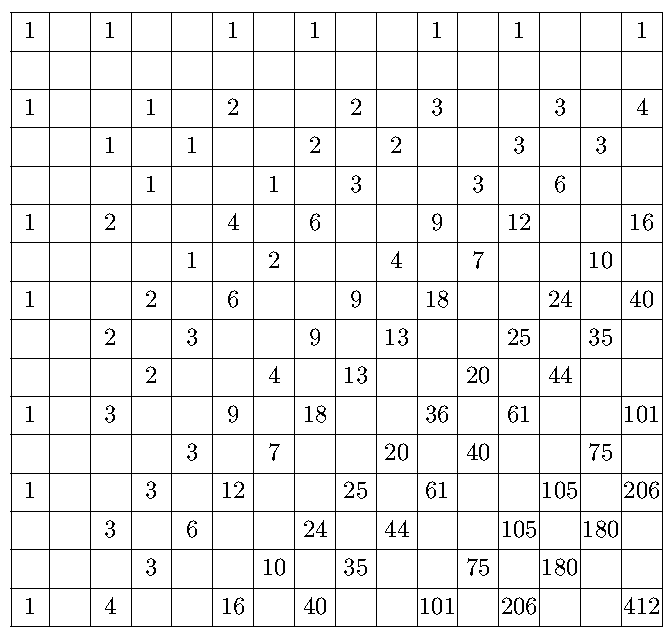
\includegraphics{obrazky/62D1}
\end{center}
Rovnako ako v~prvom riešení prichádzame k~výsledku 412.\\
\\
\begin{tcolorbox}[breakable,notitle,boxrule=0pt,colback=light-gray,colframe=light-gray]\ul{24.8} [61-I-6]
Na hracej ploche $n \times n$ tvorenej bielymi štvorcovými políčkami sa Monika a Tamara striedajú v~ťahoch jednou figúrkou pri nasledujúcej hre. Najskôr Monika položí figúrku na ľubovoľné políčko a toto políčko zafarbí namodro. Ďalej vždy hráčka, ktorá je na ťahu, urobí s~figúrkou skok na políčko, ktoré je doposiaľ biele, a toto políčko zafarbí namodro. Pritom pod skokom rozumieme bežný ťah šachovým jazdcom,  t.\,j. presun figúrky o~dve políčka zvislo alebo vodorovne a súčasne o~jedno políčko v~druhom smere. Hráčka, ktorá je na rade a už nemôže urobiť ťah, prehráva. Postupne pre $n = 4, 5, 6$ rozhodnite, ktorá z~hráčok môže hrať tak, že vyhrá nezávisle na ťahoch druhej hráčky.

\end{tcolorbox}

\rieh Ak je celkový počet políčok hracej plochy párny (v~zadaní pre $n = 4$ a $n = 6$), môže v~poradí druhá hráčka pomýšľať na túto víťaznú stratégiu: spárovať všetky políčka hracej dosky do dvojíc tak, aby v~každom páre boli políčka navzájom dosiahnuteľné jedným skokom. Pokiaľ také spárovanie políčok druhá hráčka nájde, má víťaznú stratégiu: v~každom ťahu urobí skok na druhé políčko toho páru, na ktorého prvom políčku figúrka práve leží.

Ak je celkový počet políčok hracej plochy nepárny (v~zadaní pre $n = 5$), môže v~poradí prvá hráčka pomýšľať na túto víťaznú stratégiu: spárovať všetky políčka hracej dosky okrem jedného do dvojíc tak, aby v~každom páre boli políčka navzájom dosiahnuteľné jedným skokom. Pokiaľ také spárovanie prvá hráčka nájde, má víťaznú stratégiu: v~prvom ťahu položí figúrku na (jediné) nespárované políčko a v~každom
ďalšom ťahu urobí skok na druhé políčko toho páru, na ktorého prvom políčku figúrka práve leží.

Nájsť požadované spárovania políčok je pre zadané príklady ľahké a je to možné urobiť viacerými spôsobmi. Ukážme tie z~nich, ktoré majú určité črty pravidelnosti. Na obr. 1 zľava je vidno, ako je možné spárovať políčka časti hracej plochy o~rozmeroch $4\times2$; celú hraciu plochu $4 \times 4$ rozdelíme na dva také bloky a urobíme spárovanie v~každom z~nich. I~na spárovanie políčok hracej plochy $6\times 6$ môžeme využiť spárovanie v~dvoch blokoch $4 \times 2$; na obr. 1 uprostred je znázornené možné stredovo súmerné spárovanie všetkých políčok. Nakoniec na obr. 1 vpravo je príklad spárovania políčok hracej plochy $5 \times 5$ s~nespárovaným políčkom v~ľavom hornom rohu (nespárované políčko nemusí byť nutne rohové); opäť je pritom využitý jeden blok $4 \times 2$.
\begin{center}
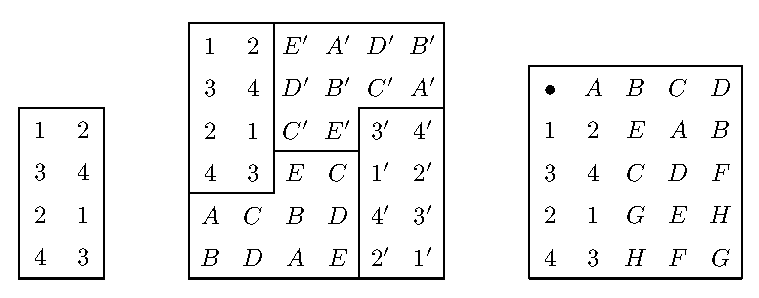
\includegraphics{obrazky/61D6} \\

Obr. 1
\end{center}


\section{Apríl}
\seminar{25}

\subsection*{Téma}
Kombinatorika II -- hry s hľadaním víťaznej stratégie a logické úlohy.
\subsection*{Ciele}
Pokračovať v precvičovaní úloh zameraných na hľadanie víťaznej stratégie a úloh, ktoré nevyžadujú špeciálne matematické znalosti.

\subsection*{Úlohy a riešenia}

% Do not delete this line (pandoc magic!)

\problem{61-I-6-N2}{seminar26}{
Na tabuli sú napísané všetky prvočísla menšie ako 100. Gitka a Terka sa striedajú v~ťahoch pri nasledujúcej hre. Najprv Gitka zmaže jedno z~prvočísel. Ďalej vždy hráčka, ktorá je na ťahu, zmaže jedno z~prvočísel, ktoré má s~predchádzajúcim zmazaným prvočíslom jednu zhodnú číslicu (tak po prvočísle 3 je možné zmazať trebárs 13 alebo 37). Hráčka, ktorá je na ťahu a nemôže už žiadne prvočíslo zmazať, prehráva. Ktorá z~oboch hráčok môže hrať tak, že vyhrá nezávisle od ťahov súperky?
}{
\rieh Pretože prvočísel menších ako 100 je nepárny počet (25), ponúka sa hypotéza, že víťaznú stratégiu bude mať prvá hráčka. Ukážme, že to tak naozaj je. Táto hráčka si vopred v~duchu spáruje (podľa spoločnej číslice) napísané prvočísla (dá sa to urobiť viacerými spôsobmi, uvedieme ten, pri ktorom v~každom kroku párujeme najmenšie doposiaľ nespárované prvočíslo s~najmenším ďalším doposiaľ nespárovaným prvočíslom so spoločnou číslicou): (2, 23), (3, 13), (5, 53), (7, 17), (11, 19), (29, 59), (31, 37), (41, 43), (47, 67), (61, 71), (73, 79), (83, 89); jediné zostávajúce nespárované prvočíslo 97 preto Gitka zmaže ako prvé a ďalej pri hre bude mazať vždy prvočíslo, ktoré je v~páre s~predchádzajúcim zmazaným prvočíslom. Týmto postupom musí vyhrať.\\
\\
\kom Úloha je malým opakovaním toho, ktoré čísla do 100 sú prvočísla a môžeme ju využiť na pripomenutie definície prvočísla. Rovnako ako aj v nasledujúcich úlohách, aj tu môžeme študentov nechať najprv odohrať niekoľko hier a potom skúsiť ich čiastkové zistenia spoločne pretaviť do univerzálnej stratégie.\\
\\
}


% Do not delete this line (pandoc magic!)

\problem{61-II-4}{
Na tabuli je napísaných prvých $n$ celých kladných čísel. Marína a Tamara sa striedajú v~ťahoch pri nasledujúcej hre. Najskôr Marína zotrie jedno z~čísel na tabuli. Ďalej vždy hráčka, ktorá je na ťahu, zotrie jedno z~čísel, ktoré sa od predchádzajúceho zotretého čísla ani nelíši o~1, ani s~ním nie je súdeliteľné. Hráčka, ktorá je na ťahu a nemôže už žiadne číslo zotrieť, prehrá. Pre $n = 6$ a pre $n = 12$ rozhodnite, ktorá z~hráčok môže hrať tak, že vyhrá nezávisle na ťahoch druhej hráčky.
}{
\rieh Úloha dvoch po sebe zotieraných čísel je v~zadanej hre symetrická: ak je po čísle $x$ možné zotrieť číslo $y$, je (pri inom priebehu hry) po čísle $y$ možné zotrieť číslo $x$. Preto si môžeme celú hru (so zadaným číslom $n$) \uv{sprehľadniť} tak, že najskôr vypíšeme všetky takéto (nazývajme ich prípustné) dvojice $(x, y)$. Keďže na poradí čísel v~prípustnej dvojici nezáleží, stačí vypisovať len tie dvojice $(x, y)$, v~ktorých $x < y$.

V~prípade $n = 6$ všetky prípustné dvojice sú
$$(1, 3), (1, 4), (1, 5), (1, 6), (2, 5), (3, 5).$$
Z~tohto zoznamu ľahko odhalíme, že víťaznú stratégiu má (prvá) hráčka Marína. Ak totiž zotrie na začiatku hry číslo 4, musí Tamara zotrieť číslo 1, a keď potom Marína zotrie číslo 6, nemôže už Tamara žiadne ďalšie číslo zotrieť. Okrem tohto priebehu $4 \rightarrow 1\rightarrow 6$ si môže Marína zaistiť víťazstvo aj inými, pre Tamaru ”vynútenými“ priebehmi, napríklad $6\rightarrow 1 \rightarrow 4$ alebo $4 \rightarrow 1 \rightarrow 3 \rightarrow 5 \rightarrow 2$.

V~prípade $n = 12$ je všetkých prípustných dvojíc výrazne väčšie množstvo. Preto si položíme otázku, či všetky čísla od 1 do 12 možno rozdeliť na šesť prípustných dvojíc. Ak totiž nájdeme takú šesticu, môžeme opísať víťaznú stratégiu druhej hráčky (Tamary): ak zotrie Marína pri ktoromkoľvek svojom ťahu číslo $x$, Tamara potom vždy zotrie to číslo $y$, ktoré s~číslom $x$ tvorí jednu zo šiestich nájdených dvojíc. Tak nakoniec Tamara zotrie aj posledné (dvanáste) číslo a vyhrá (prípadne hra skončí skôr tak, že Marína nebude môcť zotrieť žiadne číslo).

Hľadané rozdelenie všetkých 12 čísel do šiestich dvojíc naozaj existuje, napríklad
$$(1, 4), (2, 9), (3, 8), (5, 12), (6, 11), (7, 10).$$
Iné vyhovujúce rozdelenie dostaneme, keď v~predošlom dvojice (1, 4) a (6, 11) zameníme dvojicami (1, 6) a (4, 11). Ďalšie, menej podobné vyhovujúce rozdelenie je napríklad
$$(1, 6), (2, 5), (3, 10), (4, 9), (7, 12), (8, 11).$$
\textit{Záver.} Pre $n = 6$ má víťaznú stratégiu Marína, pre $n = 12$ Tamara.\\
\\
\kom Úloha je náročnejšia ako predchádzajúca, no študenti by mali prvú časť zvládnuť samostatne, v časti druhej môžu svoje sily spojiť so s ďalšími spolužiakmi, príp. stratégie, ktoré vymysleli, otestovať pri vzájomnej hre.\\
\\
}


% Do not delete this line (pandoc magic!)

\problem{61-I-6-N3}{seminar26}{
Dve hráčky majú k~dispozícii pre hru, ktorú opíšeme, neobmedzený počet dvadsaťcentových mincí a stôl s~kruhovou doskou s~priemerom 1\,m. Hra prebieha tak, že sa hráčky pravidelne striedajú v~ťahoch. Najprv prvá hráčka položí jednu mincu kamkoľvek na prázdny stôl. Ďalej vždy hráčka, ktorá je na ťahu, položí na voľnú časť stola ďalšiu mincu (tak, aby nepresahovala okraj stola a aby sa skôr položených mincí nanajvýš dotýkala). Ktorá z~oboch hráčok môže hrať tak, že vyhrá nezávisle od ťahov súperky?
}{
\rieh Víťaznú stratégiu má prvá hráčka: prvú mincu položí doprostred stola a v~každom ďalšom kroku položí mincu na miesto súmerne združené podľa stredu stola s~miestom práve položenej mince.\\
\\
\kom Úloha je zaujímavým príkladom, kde zohráva špeciálnu úlohu jeden konkrétny bod hracej plochy. Nájdenie víťaznej stratégie je po uvedomení si tejto vlastnosti už úlohou jednoduchou. Na príklade tejto hry môžeme študentov upozorniť na ďalší všeobecný princíp, ktorý pri riešení matematických problémov môže prísť vhod -- hľadanie symetrií, príp. špeciálnych bodov týchto symetrií a skúmanie ich vlastností, pričom symetrie nemusíme chápať nutne iba v geometrickom kontexte. \\
\\
}


% Do not delete this line (pandoc magic!)

\problem{59-D-1}{
Erika a Klárka hrali hru ”slovný logik“ s týmito pravidlami: Hráč $A$ si myslí slovo zložené z piatich rôznych písmen. Hráč $B$ vysloví ľubovoľné slovo zložené z piatich rôznych písmen a hráč $A$ mu prezradí, koľko písmen uhádol na správnej pozícii a koľko na nesprávnej. Písmená považujeme za rôzne, aj keď sa líšia iba mäkčeňom alebo dĺžňom (napríklad písmena $A$, \textit{Á} sú rôzne). Keby si hráč $A$ myslel napríklad slovo \textit{LOĎKA} a $B$ by vyslovil slovo \textit{KOLÁČ}, odpovie hráč $A$, že jedno písmeno uhádol hráč $B$ na správnej pozícii a dve na nesprávnej. Skrátene oznámi \uv{1 + 2}, lebo sa naozaj obe slová zhodujú iba v písmene $O$ vrátane pozície (druhej zľava) a v písmenách $K$ a $L$, ktorých pozície sú odlišné. Erika si myslela slovo z piatich rôznych písmen a Klárka vyslovila slová \textit{KABÁT, STRUK, SKOBA, CESTA} a \textit{ZÁPAL}. Erika na tieto slová v danom poradí odpovedala 0 + 3, 0 + 2, 1 + 2, 2 + 0 a 1 + 2. Zistite, aké slovo si Erika mohla myslieť.
}{
\rieh Slová \textit{ZÁPAL} a $STRUK$ nemajú spoločné písmená. Preto sa, ako vyplýva z odpovedí 1 + 2 a 0 + 2, medzi ich písmenami, ktoré dokopy tvoria množinu $M= \{Z$, \textit{Á}, $P, A, L, S, T, R, U, K\}$, nachádza všetkých päť písmen hľadaného slova. V slove $SKOBA$ majú byť práve tri z hľadaných písmen. Sú to teda písmená $S, K, A$. (Zvyšné písmená $B$ a $O$ totiž do množiny $M$ nepatria.) V slove $CESTA$ majú byť len dve z hľadaných písmen, a obe na správnej pozícii. Sú to už nájdené $S$ a $A$, ktoré teda patria na tretie, resp. piate miesto hľadaného slova (a písmeno $T$ môžeme z množiny $M$ ”vylúčiť“). Písmeno $K$ nemôže byť ani na prvom, ani na druhom mieste: vyplýva to z odpovedí pre slová \textit{KABÁT} (0 + 3) a $SKOBA$ (1 + 2). Takže je na štvrtom mieste a ostáva určiť prvé dve písmená. V slove $STRUK$ sú len dve z hľadaných písmen (musia to teda byť $S$ a $K$), obe na nesprávnych pozíciách. Preto z množiny $M$ \uv{ vylúčime} aj písmená $R, U$ (a $T$, ak sme to doteraz neurobili). Zvyšné dve hľadané písmená potom patria do množiny $\{Z$, \textit{Á}, $P, L\}$. Z podmienok pre slovo \textit{KABÁT} vyplýva, že jedno z nich je \textit{Á}. V slove \textit{ZÁPAL} je práve jedno písmeno na správnej pozícii. Keby to bolo $Z$, nemali by sme kam uložiť písmeno \textit{Á}. Takže \textit{Á} je na druhom mieste a navyše môžeme vylúčiť písmeno $Z$. Na prvom mieste hľadaného slova môže byť $L$ alebo $P$. Ľahko sa presvedčíme, že nájdené slová \textit{LÁSKA} aj \textit{PÁSKA} vyhovujú všetkým podmienkam úlohy.\\
\\
\kom Úloha opäť nevyžaduje žiadne matematické znalosti, je však výbornou previerkou toho, ako sú študenti schopní narábať s veľkým množstvom informácií, nestratiť v nich prehľad a využiť ich na zdarné vyriešenie zadaného problému. \\
\\
}


\problem{63-D-6}{
Šachového turnaja sa zúčastnilo 8 hráčov a každý s každým odohral jednu partiu. Za víťazstvo získal hráč 1 bod, za remízu pol bodu, za prehru žiadny bod. Na konci turnaja mali všetci účastníci rôzne počty bodov. Hráč, ktorý skončil na 2. mieste, získal rovnaký počet bodov ako poslední štyria dokopy. Určte výsledok partie medzi 4. a 6. hráčom v celkovom poradí.
}{
\rieh Poslední štyria hráči odohrali medzi sebou 6 partií, takže počet bodov, ktoré dokopy získali, je aspoň 6. Hráč, ktorý skončil na 2. mieste, teda získal aspoň 6 bodov. Keby získal viac ako 6, teda aspoň 6,5 bodov, musel by najlepší hráč (vďaka podmienke rôznych počtov) získať všetkých 7 možných bodov; porazil by tak i hráča na 2. mieste, ktorý by v dôsledku toho získal menej ako 6,5 bodov, a to je spor. Hráč v poradí druhý preto získal práve 6 bodov. Presne toľko ale získali dokopy i poslední štyria, a tak mohli tieto body získať len zo vzájomných partií, čo znamená, že prehrali všetky partie s hráčmi z prvej polovice výsledného poradia. Hráč, ktorý skončil na 6. mieste, preto prehral partiu s hráčom, ktorý skončil na 4. mieste.\\
\\
\kom Posledná logická úloha seminára poskytuje niekoľko rôznych ciest k riešeniu, nielen jedinú popísanú v zadaní a tak môže byť pre študentov inšpiratívne svoje riešenia medzi sebou pozdieľať. Na úlohu tiež nadväzuje domáca práca.
}




\subsection*{Domáca práca}


% Do not delete this line (pandoc magic!)

\problem{63-K-2}{
{25.6}
Šachového turnaja sa zúčastnilo 5 hráčov a každý s každým odohral jednu partiu. Za prvenstvo získal hráč 1 bod, za remízu pol bodu, za prehru žiadny bod. Poradie hráčov na turnaji sa určuje podľa počtu získaných bodov. Jediným ďalším kritériom rozhodujúcim o konečnom umiestnení hráčov v prípade rovnosti bodov je počet výhier (kto má viac výhier, je na tom v umiestnení lepšie). Na turnaji získali všetci hráči rovnaký počet bodov. Vojto porazil Petra a o prvé miesto sa delil s Tomášom. Ako dopadla partia
medzi Petrom a Martinom?
}{
\rieh Každý hráč odohral po jednej partii so zvyšnými štyrmi. Bolo teda odo hraných celkom $\frac{1}{2}\cdot5 \cdot 4 = 10$ partií, takže každý hráč získal práve 2 body. Sú len tri možnosti, ako získať odohraním štyroch partií 2 body, a podľa toho obsahovala celková tabuľka nanajvýš tri rovnocenné skupiny hráčov. Tieto skupiny, $A, B$ a $C$, uvádzame v poradí, v ktorom by sa v konečnej tabuľke umiestnili:

Skupina $A$ obsahuje všetkých hráčov, ktorí majú po dvoch výhrach a dvoch prehrách. Skupina $B$ pozostáva z hráčov s jednou výhrou, jednou prehrou a dvoma remízami. Skupina $C$ obsahuje hráčov so štyrmi remízami.

Vojto a Tomáš sú jediní víťazi, preto nepatria do skupiny $C$. Nepatria ani do skupiny $B$, pretože v opačnom prípade by s nimi museli všetci traja hráči zo skupiny $C$ s horším výsledkom remizovať (a každý hráč skupiny B má len dve remízy).

Z toho vyplýva, že Vojto a Tomáš majú po dvoch výhrach a dvoch prehrách a skupina $C$ je prázdna. Zvyšní traja hráči tak majú po jednej výhre, jednej prehre a dvoch remízach, ktoré museli uhrať navzájom medzi sebou.\\
\textit{Záver}. Peter a Martin spolu remizovali.\\

\textbf{Iné riešenie.} Využijeme (nadbytočný) údaj, že Vojto porazil Petra: Keby mali Vojto a Tomáš po jednej výhre, jednej prehre a dvoch remízach, musel by aj Peter patriť medzi víťazov turnaja. Jediný v poradí nižší celkový výsledok sú totiž štyri remízy, Peter však jednu partiu prehral, a tak musel aj jednu vyhrať. Vojto a Tomáš majú 1preto po dvoch výhrach a dvoch prehrách. Ak Peter prehral s Vojtom, musel poraziť Tomáša. (Nemohol mať dve prehry, keďže bol v poradí nižšie ako Tomáš a Vojto. Ani nemohol s Tomášom, ktorý žiadnu remízu nemá, remizovať.) Potrebný druhý bod získal dvoma remízami -- s Martinom a nepomenovaným piatym hráčom.\\
\textit{Záver}. Peter a Martin spolu remizovali.\\
\\
}


\problem{64-D-3}{
Simona a Lenka hrajú hru. Pre dané celé číslo $k$ také, že $0 \leq k \leq 64$, vyberie Simona $k$ políčok šachovnice $8 \times 8$ a každé z nich označí krížikom. Lenka potom šachovnicu nejakým spôsobom vyplní tridsiatimi dvoma dominovými kockami. Ak je počet kociek pokrývajúcich dva krížiky nepárny, vyhráva Lenka, inak vyhráva Simona. V závislosti
od $k$ určte, ktoré z dievčat má vyhrávajúcu stratégiu.
}{
\rieh Riešenie rozdeľme podľa hodnoty čísla $k$.

Ak $k = 0$, je počet kociek pokrývajúcich dva krížiky rovný nule, preto vyhrá Simona.

Ak $0 < k \leq 32$, umiestni Simona krížiky napr. iba na biele políčka šachovnice. Potom pod žiadnou kockou nie sú dva krížiky, preto vyhrá Simona.

Ak $k > 32$, pričom $k$ je párne, umiestni Simona 32 krížikov na biele políčka a zvyšné krížiky kamkoľvek. Potom pod párnym počtom kociek sú dva krížiky (takých kociek je totiž práve $k - 32$, pretože každá dominová kocka pokrýva jedno biele a jedno čierne
políčko šachovnice), takže vyhrá Simona.

Ak $32 < k \leq 61$, pričom k je nepárne, nenapíše Simona krížiky do troch políčok v jednom z \uv{bielych rohov}, t. j. do rohového bieleho a do dvoch susedných čiernych políčok, ale napíše ich do všetkých ostatných 31 bielych políčok a zvyšok do akýchkoľvek čiernych políčok (okrem spomenutých dvoch). Na bielych políčkach je teda nepárny počet krížikov a na čiernych párny počet krížikov. Okolo každého čierneho políčka s krížikom sú všetky biele políčka tiež s krížikom, preto každá kocka, ktorá zakrýva čierne políčko s krížikom, zakrýva dva krížiky. Iné kocky dva krížiky nezakrývajú. Preto opäť vyhrá Simona.

Ak $k = 63$, dva krížiky nie sú iba pod jedinou kockou, preto v takom prípade vyhrá Lenka, a to bez potreby akejkoľvek stratégie.\\
\textit{Záver.} Pre každé $0 \leq k \leq 64$, $k \neq 63$, má vyhrávajúcu stratégiu Simona, pri $k = 63$ vyhráva automaticky Lenka.\\
\\
}



\subsection*{Doplňujúce zdroje a materiály}
Výborným zdrojom všemožných matematických hier, spolu s ich kategorizáciou a možnosťou využitia v triede je  [~\cite{burjan1999}].


\section*{Seminár 26}
\subsection*{Téma}
Krajské kolo MO

\subsection{Ciele}
Analyzovať so študentmi úlohy krajského kola MO, ukázať na prípadné spojitosti s kolom domácim a školským, objasniť najčastejšie chyby.


\seminar{27}{Krajské kolo MO}
\teachernote{
\subsection*{Ciele}
Analyzovať so študentmi úlohy krajského kola MO, ukázať na prípadné spojitosti s kolom domácim a školským, objasniť najčastejšie chyby.
}
\seminar{28}{Hra SET}

\teachernote{
\subsection*{Ciele}
Zoznámenie sa s hrou SET a riešenie jednoduchších aj zložitejších úloh využívajúcich vlastnosti herných kartičiek.



\subsubsection*{Úvodný komentár}

Seminár má trochu odlišnú štruktúru, než na akú boli študenti v seminároch doteraz navyknutí, no nepovažujeme to za žiadny problém. Taktiež je tento a nasledujúci seminár zaradený ako odľahčenie po tom, čo matematická olympiáda kategórie C vyvrcholila v uplynulom týždni.

\subsection*{Priebeh seminára}

\subsubsection*{Kartičky v hre SET}

Hra SET je kartovou hrou pre dvoch a viac hráčov. Každá kartička zobrazuje sadu symbolov, ktorá má 4 charakteristiky, pričom každá sa vyskytuje v~troch variantoch:
\begin{enumerate}
\item \textit{farba}: červená, modrá, zelená;
\item  \textit{tvar}: obdĺžnik, ovál, trojuholník;
\item \textit{výplň}: plná, polovičná, úplne biela;
\item \textit{počet symbolov}: jeden, dva, tri.
\end{enumerate}

\begin{tcolorbox}[breakable,notitle,boxrule=0pt,colback=light-gray,colframe=light-gray]\ul{30.1} Koľko kariet obsahuje hrací balíček? \end{tcolorbox}
\rie Keďže každá zo 4 charakteristík sa môže vyskytnúť v~troch rôznych variantoch, v~balíčku je celkom $3^4=81$ rôznych kartičiek. \\
\\
\kom Na seminár je vhodné mať kartičky nastrihané a zalaminované, aby sa s~nimi študentom lepšie manipulovalo. Príklad kartičiek je v prílohe.

\subsubsection*{Zoznámenie sa s~hrou SET}
SET je trojica kartičiek, pre ktorú platí: každá z~charakteristík je buď pre všetky tri kartičky rovnaká, alebo je na každej kartičke odlišná. Ak sa napríklad pozrieme na charakteristiku \textit{tvar}, tak sú na všetkých troch kartičkách buď len samé ovály (alebo len samé obdĺžniky, alebo len samé trojuholníky), alebo sú na jednej kartičke ovály, na druhej obdĺžniky a na tretej trojuholníky. Podobne pre ďalšie charakteristiky. \\
\\ \vspace{10pt}
\noindent
\begin{minipage}{.4\textwidth}
\includegraphics[width=0.8\textwidth]{images/set_ano.png}\\
Táto trojica kartičiek tvorí SET: farba je rovnaká, tvar je na každej kartičke iný, podobne výplň a všetky majú rovnaký počet symbolov. \\
\\

\end{minipage}% This must go next to `\end{minipage}`
\hspace{20pt}\begin{minipage}{.4\textwidth}
\includegraphics[width=0.8\textwidth]{images/set_nie.png}\\
Táto trojica nie je SET. Síce majú všetky tri kartičky rovnaký počet symbolov, symboly sú rovnakého tvaru a každá kartička je inej farby, výplň na dvoch kartičkách je prázdna zatiaľ čo tretia je vyplnená polovične.
\end{minipage}

Po zamiešaní sa z~balíčka vyloží na stôl 12 kartičiek. Hráči medzi nimi hľadajú SETy. Ak sa to niekomu podarí, vykríkne \uv{SET!} a ukáže ho spoluhráčom. Ak je SET správny, hráč si ho vezme zo stola, namiesto neho sa vyložia nové tri kartičky a pokračuje sa v~hre. V~prípade, že sú hráči presvedčení, že sa medzi vyloženými kartičkami žiadny SET nenachádza, doložia na stôl ďalšie tri kartičky. Hra končí v~momente, kedy hráči vyčerpajú všetky kartičky. Cieľom hry je, samozrejme, pozbierať čo najviac SETov. Hra sa dá hrať v~takmer ľubovoľne veľkej skupine, z~praktických dôvodov sa najviac osvedčili trojice a štvorice.\\
\\
\kom Predtým, než sa pustíme do hrania, je vhodné so študentmi prejsť niekoľko trojíc kartičiek a pobaviť sa o~tom, ktoré trojice SETmi sú, ktoré nie a prečo, prípadne premietnuť rozloženie 12 kartičiek a hľadať v~nich SETy spoločne. \\
\\
Po zahraní niekoľkých kôl sa so študentmi pobavíme o~tom, akým spôsobom SETy hľadali, ktoré SETy sú na nájdenie jednoduchšie, prípadne iné ďalšie zaujímavosti, ktoré počas hry vypozorovali. K~tejto diskusii sa môžeme vrátiť neskôr v~priebehu seminára, keď sa budeme zaoberať kategorizovaním rôznych typov SETov.

\subsubsection*{Úlohy o~balíčku kariet}
\begin{tcolorbox}[breakable,notitle,boxrule=0pt,colback=light-gray,colframe=light-gray]\ul{30.2} Ak vyberiem dve ľubovoľné kartičky z~balíčka, koľko kartičiek existuje takých, aby s~pôvodnými dvoma tvorili SET a prečo? \end{tcolorbox}

\rie Taká kartička je práve jedna, keďže charakteristiky prvých dvoch priamo určujú, aká variácia každej charakteristiky musí byť na poslednej kartičke (ak sa prvé dve kartičky v~charakteristike zhodujú, musí sa s~nimi zhodovať aj tretia, ak sú odlišné, aj tretia kartička sa musí odlišovať).\\
\\
\begin{tcolorbox}[breakable,notitle,boxrule=0pt,colback=light-gray,colframe=light-gray]\ul{30.3} Koľko rôznych SETov (kartičky sa v~rámci jednotlivých SETov môžu opakovať) sa nachádza v~celom balíčku?\end{tcolorbox}

\rie  Na vytvorenie SETu potrebujeme tri kartičky. Prvú z~nich môžem bez akéhokoľvek obmedzenia vybrať spomedzi všetkých 81 kartičiek, druhá kartička sa dá vybrať 80 spôsobmi a z~predchádzajúceho vieme, že tretia kartička tvoriaca SET s~už dvoma zvolenými je práve jedna. Keďže však nezáleží na poradí, v~ktorom sme kartičky vyberali, vydelíme počet možností $81\cdot80$ počtom všetkých možných usporiadaní troch kartičiek, teda $6$. Celkom dostávame $\frac{81\cdot80}{6}=1080$ rozličných SETov.\\
\\
\begin{tcolorbox}[breakable,notitle,boxrule=0pt,colback=light-gray,colframe=light-gray]\ul{30.4} Z~balíčka vyberieme jednu kartičku. Koľkých rôznych SETov môže byť táto kartička súčasťou?\end{tcolorbox}
\rie  Z~predchádzajúceho plynie, že zvyšných 80 kartičiek v~balíčku vieme rozdeliť na 40 neprelínajúcich sa dvojíc, pričom každá táto dvojica bude tvoriť s~pôvodnou kartičkou SET.\\
\\
\kom Menej zdatným študentom môže s~pochopením vysvetlenia pomôcť vyložiť si na stôl konkrétne dvojice -- teda hľadať konkrétne SETy, ktorých je vybraná kartička súčasťou. \\
\\
\begin{tcolorbox}[breakable,notitle,boxrule=0pt,colback=light-gray,colframe=light-gray]\ul{30.5} Ako je možné ukázať, že v~danom rozložení kartičiek na stole sa nenachádza žiadny SET?\end{tcolorbox}
\rie  K~tomuto problému je možné pristupovať rôznymi spôsobmi, no všetky spája potreba skontrolovať všetky možné kombinácie a vylúčiť prítomnosť SETu. Zaujímavé je pozorovať, akú stratégiu študenti zvolia (v~porovnaní s~tým, ako postupovali pri hraní hry).  Nástavbou na túto úlohu môže byť otázka, ako dané rozloženie 12 kartičiek  skontrolovať čo najefektívnejšie.\\
\\

\begin{tcolorbox}[breakable,notitle,boxrule=0pt,colback=light-gray,colframe=light-gray]\ul{30.6} Je možné SETy nejako kategorizovať? Ako? Koľko SETov v~jednotlivých kategóriách je možné vytvoriť? Vieme správnosť našich výpočtov overiť pomocou nejakých predchádzajúcich úvah?\end{tcolorbox}
\rie Táto úloha sa dá opäť uchopiť mnohými spôsobmi. Jedným z~nich môže byť roztriedenie SETov pomocou počtu charakteristík, ktoré majú kartičky spoločné. Každé rozdelenie, ktoré žiaci vymyslia, by ich však v~konečnom dôsledku malo priviesť k~rovnakému počtu SETov ako v~úlohe 2.\\
\\
\textbf{Záverečný komentár.} Hra SET je pre študentov (a nielen nich) veľmi atraktívna a majú tendencie sa odhodlane púšťať aj do predkladaných problémov. Stretnutie je tak príjemnou zmenou tempa a obsahu doterajšieho priebehu seminára

\subsubsection*{Doplňujúce zdroje a materiály}

Výborným sprievodcom plným zaujímavých úloh spolu s komentovanými študentskými riešeniami je možné nájsť na \cite{SET}.


}



\section{Máj}
%\seminar{29}

\subsection*{Téma}
Algebra -- Kvadratické rovnice

\teachernote{
\subsection*{Ciele}
Precvičiť metódy používané pri práci s~kvadratickými rovnicami

}
\subsection*{Úlohy a riešenia}

\problem{57-I-5}{
Určte všetky dvojice $a, b$ reálnych čísel, pre ktoré má každá z~kvadratických rovníc
$$ax^2 + 2bx + 1 = 0, \ \ \ \ bx^2 + 2ax + 1 = 0$$
dva rôzne reálne korene, pričom práve jeden z~nich je spoločný obom rovniciam.
}{
\rieh Zo zadania vyplýva, že a $6\neq 0$, $b \neq 0$ (inak by rovnice neboli kvadratické)
a $a \neq b$ (inak by rovnice boli totožné, a ak by mali dva reálne korene, boli by oba
spoločné).

Označme $x_0$ spoločný koreň oboch rovníc, takže
$$ax_0^2+ 2bx_0 + 1 = 0,\ \ \ bx_0^2+ 2ax_0 + 1 = 0.$$
Odčítaním oboch rovníc dostaneme $(a - b)(x_0^2- 2x_0 ) = x_0 (a - b)(x_0 - 2) = 0$. Keďže $a \neq b$ a 0 zrejme koreňom daných rovníc nie je, musí byť spoločným koreňom číslo $x_0 = 2$. Dosadením do daných rovníc tak dostaneme jedinú podmienku $4a + 4b + 1 = 0$, čiže
$$b = -a -\frac{1}{4}.$$


Diskriminant druhej z~daných rovníc je potom $4a^2 - 4b = 4a^2 + 4a + 1 = (2a + 1)^2$, takže rovnica má dva rôzne reálne korene pre ľubovoľné $a \neq -\frac{1}{2}$. Podobne diskriminant prvej z~daných rovníc je $4b^2- 4a = 4b^2 + 4b +1 = (2b +1)^2$. Rovnica má teda dva rôzne reálne korene pre ľubovoľné $b \neq -\frac{1}{2}$, čiže $a\neq  \frac{1}{4}$

Z~uvedených predpokladov však zároveň vyplýva $a \neq -\frac{1}{4}$ $(b \neq 0)$ a $a \neq - \frac{1}{8}$ $(a \neq b)$.

\textit{Záver.} Vyhovujú všetky dvojice $(a, -a - \frac{1}{4})$, kde $a \in \RR \ \{-\frac{1}{2}, -\frac{1}{4}, -\frac{1}{8}, 0, \frac{1}{4}\}$.\\
}


\problem{57-S-5}{
Určte všetky dvojice $(a, b)$ reálnych čísel, pre ktoré majú rovnice
$$x^2 + (3a + b)x + 4a = 0, \ \ \ \  x^2 + (3b + a)x + 4b = 0$$
spoločný reálny koreň.
}{
\rieh Nech $x_0$ je spoločný koreň oboch rovníc. Potom platí
$$x_0^2+ (3a + b)x_0 + 4a = 0, \ \ \ \  x_0^2+ (3b + a)x_0 + 4b = 0.$$
Odčítaním týchto rovníc dostaneme $(2a-2b)x_0 +4(a-b) = 0$, odkiaľ po úprave získame $(a - b)(x_0 + 2) = 0$.

Rozoberieme dve možnosti:

Ak $a = b$, majú obidve dané rovnice rovnaký tvar $x^2 + 4ax + 4a = 0$. Aspoň jeden koreň (samozrejme spoločný) existuje práve vtedy, keď je diskriminant $16a^2-16a$ nezáporný, teda $a \in (-\infty, 0\rangle \cup \langle 1, \infty)$.

Ak $x_0 = -2$, dostaneme z~prvej aj z~druhej rovnice $4-2a-2b = 0$, teda $b = 2-a$. Dosadením do zadania dostaneme rovnice
$$x^2 + (2a + 2)x + 4a = 0, \ \ \ \ x^2 + (6-2a)x + 8-4a = 0,$$
ktoré majú pri ľubovoľnej hodnote parametra a spoločný koreň $-2$.

\textit{Záver.} Dané rovnice majú aspoň jeden spoločný koreň pre všetky dvojice $(a, a)$, kde $a \in (-\infty, 0\rangle \cup \langle 1, \infty)$, a pre všetky dvojice tvaru $(a, 2-a)$, kde $a$ je ľubovoľné.\\
\\
\ul{30.3} [57-II-1]  Uvažujme dve kvadratické rovnice
$$x^2-ax-b = 0,\ \ \ \  x^2-bx-a = 0$$
s~reálnymi parametrami $a$, $b$. Zistite, akú najmenšiu a akú najväčšiu hodnotu môže nadobudnúť súčet $a + b$, ak existuje práve jedno reálne číslo $x$, ktoré súčasne vyhovuje obom rovniciam. Určte ďalej všetky dvojice $(a, b)$ reálnych parametrov, pre ktoré tento súčet tieto hodnoty nadobúda.

\rieh Odčítaním oboch daných rovníc dostaneme rovnosť $(b-a)x+a-b = 0$, čiže $(b-a)(x-1) = 0$. Odtiaľ vyplýva, že $b = a$ alebo $x = 1$.

Ak $b = a$, majú obidve rovnice tvar $x^2-ax-a = 0$. Práve jedno riešenie existuje práve vtedy, keď diskriminant $a^2 + 4a$ je nulový. To platí pre $a = 0$ a pre $a = -4$. Pretože $b = a$, má súčet $a + b$ v~prvom prípade hodnotu $0$ a v~druhom prípade hodnotu $-8$.

Ak $x = 1$, dostaneme z~daných rovníc $a + b = 1$, teda $b = 1-a$. Rovnice potom majú tvar
$$x^2-ax + a-1 = 0 \ \ \ \ \text{a} \ \ \ \ x^2 + (a-1)x-a = 0.$$
Prvá má korene $1$ a $a-1$, druhá má korene $1$ a $-a$. Práve jedno spoločné riešenie tak dostaneme vždy s~výnimkou prípadu, keď $a-1 = -a$, čiže $a = \frac{1}{2}$ -- vtedy sú spoločné riešenia dve.

\textit{Záver.} Najmenšia hodnota súčtu $a + b$ je $-8$ a je dosiahnutá pre $a = b = -4$. Najväčšia hodnota súčtu $a + b$ je $1$; túto hodnotu má súčet $a + b$ pre všetky dvojice $(a, 1-a)$, kde $a\neq \frac{1}{2}$ je ľubovoľné reálne číslo.\\
\\
}


\problem{59-I-6}{
Reálne čísla $a$, $b$ majú túto vlastnosť: rovnica $x^2 -ax+b-1 = 0$ má v~množine reálnych čísel dva rôzne korene, ktorých rozdiel je kladným koreňom rovnice $x^2 - ax + b + 1 = 0$.

a) Dokážte nerovnosť $b > 3$.

b) Pomocou $b$ vyjadrite korene oboch rovníc.
}{
\rieh  Označme $x_1$ menší a $x_2$ väčší koreň prvej rovnice. Potom platí $x_1 + x_2 = a$, $x_1 x_2 = b - 1$. Druhá rovnica má koreň $x_2 - x_1$, a keďže súčet oboch koreňov je $a$, musí byť druhý koreň $a - (x_2 - x_1 ) = x_1 + x_2 - x_2 + x_1 = 2x_1$. Súčin koreňov druhej rovnice je $(x_2 -x_1 )\cdot2x_1 = b+1$. Odtiaľ dostávame $b = -1+2x_1 x_2 -2x_1^2= -1+2(b-1)-2x_1^2$, a teda
$$b = 3 + 2x_1^3> 3, \ \ \ \  (1)$$
lebo z~rovnosti $x_1 = 0$ by vyplývalo $b + 1 = b - 1 = 0$.

Keďže $x_2 - x_1 > 0$ a $b + 1 > 0$, musí byť aj $x_1 > 0$; z~(1) máme $x_1 =\sqrt{(b - 3)/2}$ a ďalej
$$x_2 =\frac{b-1}{x_1}=\frac{(b - 1)\sqrt{2}}{\sqrt{b-3}}.$$
Korene druhej rovnice sú potom
$$x_2 - x_1 = \frac{b+1}{} \ \ \ \ \text{a} \ \ \ \  2x_1=\sqrt{2(b - 3)}.$$
\\
\textbf{Iné riešenie}. Korene prvej rovnice sú
$$x_1 = \frac{a -\sqrt{a^2 - 4b + 4}}{2}, \ \ \ \  x_2 =\frac{a +\sqrt{a^2 - 4b + 4}}{2},$$
pričom pre diskriminant máme
$$D = a^2 - 4(b - 1) > 0. \ \ \ \  (2)$$
Rozdiel koreňov $x_2 - x_1 =\sqrt{a^2 - 4b + 4}$ je koreňom druhej rovnice, a preto
\begin{align*}
a^2 - 4b + 4 - a \sqrt{a^2 - 4b + 4} + b + 1 &= 0,\\
a^2 - 3b + 5 &= a\sqrt{a 2 - 4b + 4}, \ \ \ \  (3)\\
a^4 + 2a^2 (5 - 3b) + (3b - 5)^2 &= a^4 - 4a^2 b + 4a^2,\\
(3b - 5)^2 &= a^2 (2b - 6).
\end{align*}
Rovnosť  $a = 0$ nastáva práve vtedy, keď $3b - 5 = 0$; potom by ale neplatilo (2). Preto $a^2 > 0$, $(3b - 5)^2 > 0$, a teda aj $2b - 6 > 0$, čiže $b > 3$. Z~(2) a (3) potom vyplýva $a > 0$, a teda $a = (3b - 5)/\sqrt{2(b - 3)}$; ďalej potom
\begin{align*}
x_1 &=\frac{1}{2}\bigg( \frac{3a-5}{\sqrt{2(b-3)}}-\sqrt{\frac{(3b-5)^2}{2(b-3)}}-4b+4\bigg)=\sqrt{\frac{b-3}{2}},\\
x_2 &=\frac{1}{2} \bigg( \frac{3a-5}{\sqrt{2(b-3)}}+\sqrt{\frac{(3b-5)^2}{2(b-3)}}-4b+4\bigg)=\frac{(b-1)\sqrt{2}}{\sqrt{b-3}}.
\end{align*}
Druhá rovnica má korene
\begin{align*}
x_3 &=\frac{a-\sqrt{a^2-4b-4}}{2}=\frac{b+1}{\sqrt{2(b-3)}}=x_2-x_1\\
x_4 &=\frac{a+\sqrt{a^2-4b-4}}{2}=\sqrt{2(b-3)}.
\end{align*}
}


% Do not delete this line (pandoc magic!)

\problem{59-S-1}{

}{
}

% Do not delete this line (pandoc magic!)

\problem{B-62-II-1}{}{
Pre ľubovoľné reálne čísla $k\neq \pm 1$, $p \neq 0$ a $q$ dokážte tvrdenie: Rovnica
$$x^2+ px + q = 0$$
má v~obore reálnych čísel dva korene, z~ktorých jeden je $k$-násobkom druhého, práve vtedy, keď platí $kp^2 = (k~+ 1)^2 q$.
}{
\rieh Čísla $x_1$, $x_2$ sú koreňmi danej kvadratickej rovnice práve vtedy, keď platí
\begin{equation} \label{eq:B62II1}
    x_1 + x_2 = -p \ \ \ \ \text{a} \ \ \ \  x_1 x_2 = q.
\end{equation}
Predpokladajme, že daná kvadratická rovnica má reálne korene $x_1 = \alpha$, $x_2 = k\alpha$. Dosadením do~\ref{eq:B62II1} dostaneme $(k + 1)\alpha = -p$ a $k\alpha^2 = q$. Pre obe strany dokazovanej rovnosti $kp^2 = (k~+ 1)^2 q$ odtiaľ vyplýva
$$kp^2= k(-(k + 1)\alpha)^2= k(k + 1)^2\alpha^2,$$
$$(k + 1)^2q = (k~+ 1)^2 \cdot k\alpha^2= k(k + 1)^2\alpha^2,$$
teda daná rovnosť skutočne platí.

Nech naopak pre reálne čísla $p$, $q$ a $k \neq -1$ platí $kp^2 = (k+1)^2q$. Uvažujme dvojicu
reálnych čísel
$$x_1 =\frac{-kp}{k + 1} \ \ \ \ \text{a} \ \ \ \  x_2 =\frac{-p}{k + 1}.$$
Také čísla (pre ktoré platí $x_1 = kx_2$) sú koreňmi danej kvadratickej rovnice, ak spĺňajú obe rovnosti~\ref{eq:B62II1}. Overenie urobíme dosadením:
\begin{align*}
x_1 + x_2 &= \frac{-kp}{k + 1}+\frac{-p}{k + 1}=\frac{-(k + 1)p}{k + 1}= -p,\\
x_1 x_2 &=\frac{-kp}{k + 1}\cdot\frac{-p}{k + 1}=\frac{kp^2}{(k + 1)^2}=\frac{(k + 1)^2q}{(k + 1)^2}= q.
\end{align*}
Tým je celý dôkaz hotový.\\
\\
}


% Do not delete this line (pandoc magic!)

\problem{B-64-II-4}{seminar30,kvadr,hra,krajskekolo}{
Na tabuli je zoznam čísel $1, 2, 3, 4, 5, 6$ a \uv{rovnica}
$$\frac{\fbox{$\phantom{7}$}}{\fbox{$\phantom{7}$}}x^2+\frac{\fbox{$\phantom{7}$}}{\fbox{$\phantom{7}$}}x + \frac{\fbox{$\phantom{7}$}}{\fbox{$\phantom{7}$}}= 0.$$
Marek s~Tomášom hrajú nasledujúcu hru. Najskôr Marek vyberie ľubovoľné číslo zo zoznamu, napíše ho do jedného z~prázdnych políčok v~\uv{rovnici} a číslo zo zoznamu zotrie. Potom Tomáš vyberie niektoré zo zvyšných čísel, napíše ho do iného prázdneho políčka a v~zozname ho zotrie. Nato Marek urobí to isté a nakoniec Tomáš doplní tri zvyšné čísla na tri zvyšné voľné políčka v~\uv{rovnici}. Marek vyhrá, ak vzniknutá kvadratická rovnica s~racionálnymi koeficientmi bude mať dva rôzne reálne korene, inak vyhrá Tomáš. Rozhodnite, ktorý z~hráčov môže vyhrať nezávisle na postupe druhého
hráča.
}{
\rieh Označme $a$, $b$, $c$ koeficienty výslednej rovnice $ax^2 + bx + c = 0$. Tá má dva rôzne reálne korene práve vtedy, keď je jej diskriminant (v~symbolickej podobe)
$$b^2 - 4ac =\bigg( \frac{{\fbox{$\phantom{7}$}}}{{\fbox{$\phantom{7}$}}} \bigg)^2-4\bigg( \frac{{\fbox{$\phantom{7}$}}}{{\fbox{$\phantom{7}$}}}\bigg) \bigg(\frac{{\fbox{$\phantom{7}$}}}{{\fbox{$\phantom{7}$}}}\bigg)$$
kladný.

Ukážeme, že vyhrávajúcu stratégiu má Marek. Najskôr do menovateľa zlomku pre koeficient $b$ napíše $1$.
\begin{enumerate}[a)]
\item Ak Tomáš obsadí vo svojom prvom ťahu iné miesto ako v~čitateli $b$, napíše do neho Marek v~nasledujúcom ťahu najväčšie zostávajúce číslo zo zoznamu (teda 5 alebo 6). Hodnota $b^2$ potom bude aspoň 25 a zo zvyšných čísel možno zostaviť výraz $4ac$ s~hodnotou nanajvýš $4\cdot  \frac{6\cdot4}{3\cdot2}= 16$. Diskriminant vzniknutej kvadratickej rovnice tak bude určite kladný.
\item Predpokladajme, že Tomáš vo svojom ťahu doplní čitateľa $b$. Marek potom v~druhom ťahu napíše najmenšie zostávajúce číslo zo zoznamu (2 alebo 3) do čitateľa $a$ (alebo $c$).
\begin{enumerate}[(i)]
\item V~prípade, že Tomáš v~prvom ťahu napísal do čitateľa $b$ číslo 2, je hodnota $b^2$ rovná 4 a najväčšia možná hodnota $4ac$ (s~prihliadnutím na druhý Marekov ťah) je $4 \cdot \frac{3\cdot 6}{4\cdot 5}=\frac{18}{5}\leq  4$, teda diskriminant vzniknutej kvadratickej rovnice bude opäť kladný.
\item  V~prípade, že Tomáš v~prvom ťahu napísal do čitateľa $b$ iné číslo ako 2, je hodnota $b^2$ aspoň 9 a hodnota $4ac$ je nanajvýš $4 \cdot \frac{2\cdot 6}{3\cdot4} = 4$, takže diskriminant
vzniknutej kvadratickej rovnice bude aj v~tomto prípade kladný.

\end{enumerate}
\end{enumerate}
\textit{Záver.} V~danej hre môže vyhrať Marek nezávisle na ťahoch Tomáša. Jeho víťazná stratégia je opísaná vyššie.\\
\\
\kom Posledná úloha je zaujímavým spojením hľadania víťaznej stratégie a analýzy vlastností diskriminantu kvadratickej rovnice. Študentov necháme riešenie úlohy hľadať samostatne a potom ich vyzveme, aby stratégiu, ktorú našli, použili pri hre so spolužiakmi. Bude zaujímavé pozorovať, či nastane situácia, v ktorej aj neoptimálna stratégia zvíťazí.\\
\\
}




\subsection*{Domáca práca}

Úlohou študentov bude vyhľadať, skonzultovať a zaslať vedúcemu seminára jeden príklad, problém alebo úlohu, ktorá sa viaže k témam algebry a teórie čísel, ktorými sme sa v seminári zaberali. Tieto úlohy budú použité ako zadania, ktoré využijeme v nasledujúcom seminári. Študenti môžu hľadať inšpiráciu v starších kolách MO, rôznych knižných publikáciách, zbierkach korešpondenčných seminárov alebo môžu úlohu dokonca sami vymyslieť.


\teachernote{
\subsection*{Doplňujúce zdroje a materiály}



} % Seminar chyba!
\seminar{30}


\subsection*{Téma}
Hra SET

\teachernote{
\subsection*{Ciele}
Zoznámenie sa s hrou SET a riešenie jednoduchších aj zložitejších úloh využívajúcich vlastnosti herných kartičiek.

\subsection*{Priebeh seminára}

\textbf{Úvodný komentár.} Seminár má trochu odlišnú štruktúru, než na akú boli študenti v seminároch doteraz navyknutí, no nepovažujeme to za žiadny problém. Taktiež je tento a nasledujúci seminár zaradený ako odľahčenie po tom, čo matematická olympiáda kategórie C vyvrcholila v uplynulom týždni.

\subsubsection*{Kartičky v hre SET}

Hra SET je kartovou hrou pre dvoch a viac hráčov. Každá kartička zobrazuje sadu symbolov, ktorá má 4 charakteristiky, pričom každá sa vyskytuje v~troch variantoch:
\begin{enumerate}
\item \textit{farba}: červená, modrá, zelená;
\item  \textit{tvar}: obdĺžnik, ovál, trojuholník;
\item \textit{výplň}: plná, polovičná, úplne biela;
\item \textit{počet symbolov}: jeden, dva, tri.
\end{enumerate}

\begin{tcolorbox}[breakable,notitle,boxrule=0pt,colback=light-gray,colframe=light-gray]\ul{30.1} Koľko kariet obsahuje hrací balíček? \end{tcolorbox}
\rie Keďže každá zo 4 charakteristík sa môže vyskytnúť v~troch rôznych variantoch, v~balíčku je celkom $3^4=81$ rôznych kartičiek. \\
\\
\kom Na seminár je vhodné mať kartičky nastrihané a zalaminované, aby sa s~nimi študentom lepšie manipulovalo. Príklad kartičiek je v prílohe.

\subsubsection*{Zoznámenie sa s~hrou SET}
SET je trojica kartičiek, pre ktorú platí: každá z~charakteristík je buď pre všetky tri kartičky rovnaká, alebo je na každej kartičke odlišná. Ak sa napríklad pozrieme na charakteristiku \textit{tvar}, tak sú na všetkých troch kartičkách buď len samé ovály (alebo len samé obdĺžniky, alebo len samé trojuholníky), alebo sú na jednej kartičke ovály, na druhej obdĺžniky a na tretej trojuholníky. Podobne pre ďalšie charakteristiky. \\
\\ \vspace{10pt}
\noindent
\begin{minipage}{.4\textwidth}
\includegraphics[width=0.8\textwidth]{images/set_ano.png}\\
Táto trojica kartičiek tvorí SET: farba je rovnaká, tvar je na každej kartičke iný, podobne výplň a všetky majú rovnaký počet symbolov. \\
\\

\end{minipage}% This must go next to `\end{minipage}`
\hspace{20pt}\begin{minipage}{.4\textwidth}
\includegraphics[width=0.8\textwidth]{images/set_nie.png}\\
Táto trojica nie je SET. Síce majú všetky tri kartičky rovnaký počet symbolov, symboly sú rovnakého tvaru a každá kartička je inej farby, výplň na dvoch kartičkách je prázdna zatiaľ čo tretia je vyplnená polovične.
\end{minipage}

Po zamiešaní sa z~balíčka vyloží na stôl 12 kartičiek. Hráči medzi nimi hľadajú SETy. Ak sa to niekomu podarí, vykríkne \uv{SET!} a ukáže ho spoluhráčom. Ak je SET správny, hráč si ho vezme zo stola, namiesto neho sa vyložia nové tri kartičky a pokračuje sa v~hre. V~prípade, že sú hráči presvedčení, že sa medzi vyloženými kartičkami žiadny SET nenachádza, doložia na stôl ďalšie tri kartičky. Hra končí v~momente, kedy hráči vyčerpajú všetky kartičky. Cieľom hry je, samozrejme, pozbierať čo najviac SETov. Hra sa dá hrať v~takmer ľubovoľne veľkej skupine, z~praktických dôvodov sa najviac osvedčili trojice a štvorice.\\
\\
\kom Predtým, než sa pustíme do hrania, je vhodné so študentmi prejsť niekoľko trojíc kartičiek a pobaviť sa o~tom, ktoré trojice SETmi sú, ktoré nie a prečo, prípadne premietnuť rozloženie 12 kartičiek a hľadať v~nich SETy spoločne. \\
\\
Po zahraní niekoľkých kôl sa so študentmi pobavíme o~tom, akým spôsobom SETy hľadali, ktoré SETy sú na nájdenie jednoduchšie, prípadne iné ďalšie zaujímavosti, ktoré počas hry vypozorovali. K~tejto diskusii sa môžeme vrátiť neskôr v~priebehu seminára, keď sa budeme zaoberať kategorizovaním rôznych typov SETov.

\subsubsection*{Úlohy o~balíčku kariet}
\begin{tcolorbox}[breakable,notitle,boxrule=0pt,colback=light-gray,colframe=light-gray]\ul{30.2} Ak vyberiem dve ľubovoľné kartičky z~balíčka, koľko kartičiek existuje takých, aby s~pôvodnými dvoma tvorili SET a prečo? \end{tcolorbox}

\rie Taká kartička je práve jedna, keďže charakteristiky prvých dvoch priamo určujú, aká variácia každej charakteristiky musí byť na poslednej kartičke (ak sa prvé dve kartičky v~charakteristike zhodujú, musí sa s~nimi zhodovať aj tretia, ak sú odlišné, aj tretia kartička sa musí odlišovať).\\
\\
\begin{tcolorbox}[breakable,notitle,boxrule=0pt,colback=light-gray,colframe=light-gray]\ul{30.3} Koľko rôznych SETov (kartičky sa v~rámci jednotlivých SETov môžu opakovať) sa nachádza v~celom balíčku?\end{tcolorbox}

\rie  Na vytvorenie SETu potrebujeme tri kartičky. Prvú z~nich môžem bez akéhokoľvek obmedzenia vybrať spomedzi všetkých 81 kartičiek, druhá kartička sa dá vybrať 80 spôsobmi a z~predchádzajúceho vieme, že tretia kartička tvoriaca SET s~už dvoma zvolenými je práve jedna. Keďže však nezáleží na poradí, v~ktorom sme kartičky vyberali, vydelíme počet možností $81\cdot80$ počtom všetkých možných usporiadaní troch kartičiek, teda $6$. Celkom dostávame $\frac{81\cdot80}{6}=1080$ rozličných SETov.\\
\\
\begin{tcolorbox}[breakable,notitle,boxrule=0pt,colback=light-gray,colframe=light-gray]\ul{30.4} Z~balíčka vyberieme jednu kartičku. Koľkých rôznych SETov môže byť táto kartička súčasťou?\end{tcolorbox}
\rie  Z~predchádzajúceho plynie, že zvyšných 80 kartičiek v~balíčku vieme rozdeliť na 40 neprelínajúcich sa dvojíc, pričom každá táto dvojica bude tvoriť s~pôvodnou kartičkou SET.\\
\\
\kom Menej zdatným študentom môže s~pochopením vysvetlenia pomôcť vyložiť si na stôl konkrétne dvojice -- teda hľadať konkrétne SETy, ktorých je vybraná kartička súčasťou. \\
\\
\begin{tcolorbox}[breakable,notitle,boxrule=0pt,colback=light-gray,colframe=light-gray]\ul{30.5} Ako je možné ukázať, že v~danom rozložení kartičiek na stole sa nenachádza žiadny SET?\end{tcolorbox}
\rie  K~tomuto problému je možné pristupovať rôznymi spôsobmi, no všetky spája potreba skontrolovať všetky možné kombinácie a vylúčiť prítomnosť SETu. Zaujímavé je pozorovať, akú stratégiu študenti zvolia (v~porovnaní s~tým, ako postupovali pri hraní hry).  Nástavbou na túto úlohu môže byť otázka, ako dané rozloženie 12 kartičiek  skontrolovať čo najefektívnejšie.\\
\\

\begin{tcolorbox}[breakable,notitle,boxrule=0pt,colback=light-gray,colframe=light-gray]\ul{30.6} Je možné SETy nejako kategorizovať? Ako? Koľko SETov v~jednotlivých kategóriách je možné vytvoriť? Vieme správnosť našich výpočtov overiť pomocou nejakých predchádzajúcich úvah?\end{tcolorbox}
\rie Táto úloha sa dá opäť uchopiť mnohými spôsobmi. Jedným z~nich môže byť roztriedenie SETov pomocou počtu charakteristík, ktoré majú kartičky spoločné. Každé rozdelenie, ktoré žiaci vymyslia, by ich však v~konečnom dôsledku malo priviesť k~rovnakému počtu SETov ako v~úlohe 2.\\
\\
\textbf{Záverečný komentár.} Hra SET je pre študentov (a nielen nich) veľmi atraktívna a majú tendencie sa odhodlane púšťať aj do predkladaných problémov. Stretnutie je tak príjemnou zmenou tempa a obsahu doterajšieho priebehu seminára

\subsubsection*{Doplňujúce zdroje a materiály}

Výborným sprievodcom plným zaujímavých úloh spolu s komentovanými študentskými riešeniami je možné nájsť na \todo{Kde?}.


}


\seminar{31}

\subsection*{Téma}
Geometria -- stredové, obvodové, úsekové uhly, tetivové štvoruholníky
\teachernote{
\subsection*{Ciele}

Zopakovať, príp. študentov zoznámiť s vlastnosťami stredových, obvodových a úsekových uhlov a ich využitím pri riešení úloh.


}
\subsubsection*{Úvodný komentár}

Predtým, ako sa so študentmi pustíme do riešenia úloh, je vhodné predstaviť, príp. zopakovať vlastnosti uhlov, ktorými sa budeme v seminári zaoberať. Vhodným materiálom je \cite{kadlecek1996}, kapitola 8.


\subsection*{Úlohy a riešenia}

%\todo{DOPLNIŤ komentáre.}

% Do not delete this line (pandoc magic!)

\problem{B-65-I-5-D1}{}{
Daná je tetiva $AB$ kružnice $k$ so stredom v bode $S$. Na úsečke $AB$ zvoľme bod $M$ a priesečník kružnice opísanej trojuholníku $AMS$ s kružnicou k označme $C$. Dokážte, že uhly $MCS$ a $MBS$ sú zhodné.
}{
\rieh Stačí využiť rovnosť uhlov v rovnoramennom trojuholníku $ABS$ a obvodové uhly nad $MS$ v kružnici opísanej trojuholníku $AMS$.
}


%\kom Úloha je veľmi jednoduchá, preto ju považujeme skôr za rozcvičku ako plnohodnotný matematický oriešok. Pekne však demonštruje to 

% Do not delete this line (pandoc magic!)

\problem{B-66-II-3}{}{
V rovine sú dané kružnice $k$ a $l$, ktoré sa pretínajú v bodoch $E$ a $F$. Dotyčnica ku kružnici $l$ zostrojená v bode $E$ pretína kružnicu $k$ v bode $H$ ($H \neq E$). Na oblúku $EH$ kružnice $k$, ktorý neobsahuje bod $F$, zvoľme bod $C$ ($E \neq C \neq H$) a priesečník priamky $CE$ s kružnicou $l$ označme $D$ ($D \neq E$). Dokážte, že trojuholníky $DEF$ a $CHF$
sú podobné.
}{
\rieh Z rovnosti obvodových uhlov nad tetivou $HF$ kružnice k vyplýva $|\ma HCF|= |\ma HEF|$. Uhol $HEF$ je zároveň úsekovým uhlom prislúchajúcim tetive $EF$ kružnice $l$, ktorý je však zhodný s obvodovým uhlom $EDF$ (obr.~\ref{fig:B66II3}). Celkovo tak platí
\begin{equation} \label{eq:B66II3_1}
    |\ma HCF| = |\ma HEF| = |\ma EDF|.
\end{equation}

\begin{figure}[h]
    \centering
    \includegraphics{images/B66II3\imagesuffix}
    \caption{}
    \label{fig:B66II3}
\end{figure}
Vzhľadom na to, že $CEFH$ je tetivový štvoruholník, je jeho vnútorný uhol pri vrchole $H$ zhodný s vonkajším uhlom pri jeho protiľahlom vrchole $E$. Platí teda
\begin{equation} \label{eq:B66II3_2}
    |\ma CHF| = |\ma DEF|.
\end{equation}
Z rovností \ref{eq:B66II3_1} a \ref{eq:B66II3_2} vyplýva na základe vety $uu$ podobnosť trojuholníkov $DEF$ a $CHF$. Tým je dôkaz hotový.\\
\\
\kom Úloha je relatívne jednoduchou aplikáciou poznatkov o stredových, obvodových a úsekových uhloch, preto dobe poslúži ako úvodná úloha seminára. Zároveň sa v úlohe vyskytuje spoločná tetiva dvoch kružníc, ktorá je prvkom mnohých geometrických úloh v kategórii B, takže je príjemné, že sa študenti s týmto prípadom zoznámia hneď na začiatku.
}


%\kom Úloha priamočiaro využíva poznatky, ktoré sme odvodili v začiatku seminára a taktiež zoznamuje študentov s XXX, ktorý sa v úlohách vyskytuje často, totiž spoločná tetiva dvoch kružníc XXX

% Do not delete this line (pandoc magic!)

\problem{B-65-II-2}{
Daná je úsečka $AB$, jej stred $C$ a vnútri úsečky $AB$ bod $D$. Kružnice $k(C, |BC|)$ a $m(B, |BD|)$ sa pretínajú v bodoch $E$ a $F$. Zdôvodnite, prečo je polpriamka $FD$ osou uhla $AFE$.
}{
\rieh Kružnica $k$ je Tálesovou kružnicou nad priemerom $AB$, takže trojuholník $ABF$ je pravouhlý s pravým uhlom pri vrchole $F$. Inými slovami, priamka $AF$ je kolmá 
\begin{figure}[h]
    \centering
    \includegraphics{images/B65II2_1\imagesuffix}
    \caption{}
    \label{fig:B65II2_1}
\end{figure}
na polomer $BF$ kružnice $m$, a preto sa priamka $AF$ dotýka kružnice $m$ v bode $F$ (obr.~\ref{fig:B65II2_1}). Z rovnosti úsekového uhla zovretého tetivou $DF$ s dotyčnicou $AF$ a obvodového uhla
nad tou istou tetivou máme (ako už je vyznačené na obrázku) 
$$|\ma AFD| = |\ma DEF|.$$
Zo súmernosti úsečky $EF$ podľa osi $AB$ tak vyplýva
$$|\ma AFD| = |\ma DEF| = |\ma DFE|,$$
čo znamená, že $FD$ je osou uhla $AFE$.

\textbf{Iné riešenie*.} Označme $\beta$ veľkosť uhla $ABF$ a dopočítajme veľkosti uhlov $DFE$ a $AFE$. Trojuholník $DBF$ je rovnoramenný, lebo jeho ramená $BD$ a $BF$ sú polomery kružnice $m$, preto
$$|\ma DFB| = \frac{1}{2}(180^\circ-\beta) = 90^\circ-\frac{\beta}{2}.$$
Keďže podobne aj trojuholník $EBF$ je rovnoramenný s osou $BD$, platí
$$|\ma EFB| = 90^\circ-beta.$$
Spojením oboch predchádzajúcich rovností tak dostávame
$$|\ma DFE| = |\ma DFB| - |\ma EFB| =\frac{\beta}{2}.$$
Z vlastností Tálesovej kružnice $k$ nad priemerom $AB$ vieme, že uhol $AFB$ je pravý. Pritom jeho časť uhol $EFB$ má, ako sme už zistili, veľkosť $90^\circ-\beta$, takže jeho druhá časť, uhol $AFE$, má veľkosť $\beta$, čo je presne dvojnásobok veľkosti uhla $DFE$. Tým sme dokázali, že priamka $FD$ je osou uhla $AFE$.

\textbf{Iné riešenie*.} Nad oblúkom $AE$ kružnice $k$ sa zhodujú uhly $ABE$ a $AFE$ (obr.~\ref{fig:B65II2_2}). Oblúku $DE$ kružnice $m$ prislúcha obvodový uhol $DFE$ a stredový uhol $DBE$. Spolu
tak dostávame
$$|\ma DFE| = \frac{1}{2} |\ma DBE| = \frac{1}{2}
|\ma ABE| = \frac{1}{2} |\ma AFE|,$$
čo dokazuje, že $FD$ je osou uhla $AFE$.
\begin{figure}[h]
    \centering
    \includegraphics{images/B65II2_2\imagesuffix}
    \caption{}
    \label{fig:B65II2_2}
\end{figure}
}


% Do not delete this line (pandoc magic!)

\problem{B-65-I-5}{
Vrcholy konvexného šesťuholníka $ABCDEF$ ležia na kružnici, pričom $|AB| = |CD|$. Úsečky $AE$ a $CF$ sa pretínajú v bode $G$ a úsečky $BE$ a $DF$ sa pretínajú v bode $H$. Dokážte, že úsečky $GH$, $AD$ a $BC$ sú navzájom rovnobežné. 
}{
\rieh Najskôr ukážeme, že $AD \parallel BC$. Keďže $|AB| = |CD|$, sú obvodové uhly nad tetivami $AB$ a $CD$ kružnice opísanej šesťuholníku $ABCDEF$ zhodné \todo{(obr. 3)}, teda $|\ma ADB| = |\ma DBC|$; to sú však striedavé uhly priečky $BD$ priamok $AD$ a $BC$, preto $AD \parallel BC$. Ostáva ukázať, že $GH \parallel AD$. Využitím zhodných obvodových uhlov nad tetivami \\
\\
\todo{DOPLNIŤ Obr.3}\\
\\
$AB$ a $CD$ pri vrcholoch $E$ a $F$ dostávame
$$|\ma GEH| = |\ma AEB| = |\ma CFD| = |\ma GFH|,$$
čo znamená, že body $E$, $F$, $G$ a $H$ ležia na jednej kružnici, pretože vrcholy zhodných uhlov $GEH$ a $GFH$ ležia v rovnakej polrovine s hraničnou priamkou $GH$. Z toho vyplýva, že uhly $EFH$ a $EGH$ nad jej tetivou $EH$ sú zhodné. To spolu so zhodnosťou uhlov $EFD$ a $EAD$ nad tetivou $ED$ pôvodnej kružnice \todo{(obr. 3)} vedie na zhodnosť súhlasných uhlov $EGH$ a $EAD$ priečky $AE$ priamok $GH$ a $AD$, ktoré sú teda naozaj rovnobežné. Tým je tvrdenie úlohy dokázané.
}

% Do not delete this line (pandoc magic!)

\problem{B-58-I-5}{seminar31,netrgeo,obvodove,dokaz,domacekolo}{
Trojuholníku $ABC$ je opísaná kružnica $k$. Os strany $AB$ pretne kružnicu $k$ v bode $K$, ktorý leží v polrovine opačnej k polrovine $ABC$. Osi strán $AC$ a $BC$ pretnú priamku $CK$ postupne v bodoch $P$ a $Q$. Dokážte, že trojuholníky $AKP$ a $KBQ$ sú zhodné.
}{
\rieh Označme $\alpha, \beta, \gamma$ zvyčajným spôsobom veľkosti vnútorných uhlov trojuholníka $ABC$ (obr.~\ref{fig:B58I5}). Bod $K$ leží na osi úsečky $AB$, preto $|AK| = |KB|$. Trojuholník $AKB$ je rovnoramenný so základňou $AB$, jeho vnútorné uhly pri vrcholoch $A$ a $B$ sú
\begin{figure}[h]
    \centering
    \includegraphics{images/B58I5\imagesuffix}
    \caption{}
    \label{fig:B58I5}
\end{figure}
teda zhodné. Podľa vety o obvodových uhloch sú zhodné aj uhly $BCK$ a $BAK$, resp.$ACK$ a $ABK$, preto sú zhodné aj uhly $BCK$ a $ACK$. Polpriamka $CK$ je teda osou uhla $ACB$:
$$|\ma ACK| = |\ma BCK| = \frac{\gamma}{2}.$$
Keďže bod $P$ leží na osi strany $AC$, je trojuholník $ACP$ rovnoramenný a jeho vnútorné uhly pri základni $AC$ majú veľkosť $\frac{1}{2}\gamma$, takže jeho vonkajší uhol $APK$ pri vrchole $P$ má veľkosť $\frac{1}{2}\gamma + \frac{1}{2}\gamma = \gamma$. Rovnako z rovnoramenného trojuholníka $BCQ$  odvodíme, že aj veľkosť uhla $BQK$ je $\gamma$. Podľa vety o obvodových uhloch sú zhodné uhly $ABC$ a $AKC$, teda uhol $AKC$ (čiže uhol $AKP$) má veľkosť $\beta$ a -- celkom analogicky -- uhol $BKQ$ má veľkosť $\alpha$.

V každom z trojuholníkov $AKP$ a $BKQ$ už poznáme veľkosti dvoch vnútorných uhlov ($\beta$, $\gamma$, resp. $\alpha$, $\gamma$), takže vidíme, že zostávajúce uhly $KAP$ a $KBQ$ majú veľkosti$\alpha$, resp. $\beta$.

Z predošlého vyplýva, že trojuholníky $AKP$ a $KBQ$ sú zhodné podľa vety $usu$, lebo majú zhodné strany $AK$ a $KB$ aj obe dvojice k nim priľahlých vnútorných uhlov.

K uvedenému postupu dodajme, že výpočet uhlov $KAP$ a $KBQ$ cez uhly $APK$ a $BQK$ možno obísť takto: zhodnosť uhlov $KAP$ a $BAC$ (resp. $KBQ$ a $ABC$) vyplýva zo zhodnosti uhlov $KAB$ a $PAC$ (resp. $KBA$ a $QBC$).\\
\\
\kom Posledná úloha seminára pekne kombinuje vlastnosti uhlov a zhodnosť trojuholníkov, je tak dôstojným zakončením tohto geometrického stretnutia.
}


\subsection*{Domáca práca}




\section{Jún}
\seminar{32}

\subsection*{Téma}
Opakovanie II -- opakovanie a upevňovanie poznatkov z oblasti geometrie a kombinatoriky

\teachernote{
\subsection*{Ciele}
Zopakovať získané poznatky z oblasti geometrie a kombinatoriky, precvičiť zrozumiteľné vysvetľovanie riešení spolužiakom.

\subsection*{Priebeh seminára}
Priebeh seminára je veľmi podobný uplynulému týždňu, študenti riešia vlastnú sadu úloha a za vysvetľovanie riešení sú zodpovední dodávatelia úloh.

\subsection*{Domáca práca}
Študenti budú mať za úlohu doriešiť problémy od svojich spolužiakov.

}

\seminar{33}

\subsection*{Téma}
Opakovanie I -- pohľad späť na všetko, čo sme sa naučili

\subsection*{Ciele}

Zopakovať kľúčové myšlienky, postupy a poznatky, ktoré v priebehu roka študenti získali.

\subsection*{Priebeh seminára}

%\todo{mind maps}

Študentov rozdelíme do 4 skupín a každej skupine pridelíme jednu zo študovaných oblastí (algebra, teória čísel, geometria, kombinatorika). Úlohou skupín bude vytvoriť myšlienkovú mapu, ktorá zhŕňa poznatky z priradenej oblasti -- mala by obsahovať nie len konkrétne fakty (napr. \uv{Súčet veľkostí protiľahlých vnútorných uhlov tetivového štvoruholníka je $180^\circ$.}), ale aj všeobecnejšie prístupy alebo metódy (napr. \uv{Pozor na kreslenie náčrtu.}).  Ak sa študenti ešte s myšlienkovými mapami nestretli, stručne im ich vysvetlíme, príp. ukážeme niekoľko príkladov. Na vypracovanie študentom necháme 20-30 minút. Po tomto čase jednotlivé skupiny prezentujú svoje výtvory a zvyšok osadenstva prispieva svojimi komentármi a otázkami. Na jednu skupinu si odporúčame vyhradiť aspoň 15 minút. Zaujímavé bude sledovať, či sa niektoré poznatky budú vyskytovať vo viacerých skupinách, prípadne či sa študenti budú odkazovať aj na inú oblasť, než akú spracovali.

Tento zvolený spôsob upevnenia a prepojenia poznatkov pokladáme za prínosný, pretože študentom dáva priestor premýšľať trochu iným spôsobom 


\subsection*{Doplňujúce materiály}

O myšlienkových mapách je možné nájsť viac na \url{https://www.mindmapping.com/mind-map.php} alebo \url{https://www.mindtools.com/pages/article/newISS_01.htm}, kde je tiež k dispozícii množstvo príkladov. 
O myšlienkových mapách je možné nájsť viac na \url{\detokenize{https://www.mindmapping.com/mind-map.php}} alebo \url{https://www.mindtools.com/pages/article/newISS_01.htm}, kde je tiež k dispozícii množstvo príkladov.


%Keďže seminárne stretnutie bude tentokrát najmä v réžii študentov, bude prebiehať trochu inak. Každá zo štyroch skupín predstaví svoju domácu prácu a spoločne so ostatnými študentmi 

%Úlohou učiteľa je výklad a myšlienky študentov vhodne korigovať tak, aby spoločne so študentami pokryli väčšinu oblastí. Cieľom tohto seminára nie je znova prechádzať všetky úlohy, ktoré sme doteraz so študentami vyriešili, ale skôr zopakovať všeobecné myšlienky a postupy, na ktoré je v jednotlivých oblastiach dobré myslieť.

%V prípade, že chce mať učiteľ istotu toho, že na seminári zaznejú všetky kľúčové myšlienky, môže študentov požiadať, aby mu domácu prácu zaslali v predstihu a skontrolovať, príp. doplniť ju.

%V prvej časti seminára prejdeme spolu so štyrmi skupinami základné oblasti problémov, ktorým sme sa na seminári venovali a v závere môžeme študentom nechať priestor na zdieľanie poznatkov alebo poučení, ktoré do žiadnej konkrétnej oblasti úloh nespadajú.





\chapter*{Záver}
\label{chap:zaver}
\addcontentsline{toc}{chapter}{\nameref{chap:zaver}}

V diplomovej práci sme sa venovali tvorbe prezenčného seminára pre študentov prvého ročníka strednej školy so záujmom o matematiku, konkrétnejšie príprave podrobných osnov vrátane riešených príkladov. Seminár má za cieľ podporovať študentov pri príprave na matematické súťaže, najmä matematickú olympiádu. Po tom, čo sme seminár zasadili do kontextu matematického vzdelávania stredoškolákov a preskúmali sme úlohy matematickej olympiády kategórie C v posledných desiatich rokoch, sme jednotlivé stretnutia tematicky rozdelili a doplnili o semináre konzultačné a zamerané aj na inú súťaž než olympiáda, konkrétne \textit{Náboj}.

Pri tvorbe obsahu sme sa snažili zakomponovať rôzne metódy výučby. Využili sme samostatnú i skupinovú prácu, matematické hry, tímové súťaže i prípravu obsahu seminára samotnými študentmi. To snáď prispelo k pestrosti seminára a rozvoju schopností a vedomostí študentov. Zároveň však pokladáme za dôležité poznamenať, že obsah a forma seminára nie sú jediným \uv{správnym} alebo najvhodnejším spôsobom práce so študentami a že prístupov k tejto úlohe je nespočetne mnoho. Taktiež nemá byť osnova seminára vnímaná ako nemenná dogma, ale skôr ako živý organizmus, ktorý sa väčšou alebo menšou mierou prispôsobuje potrebám konkrétnych študentov účastniacich sa konkrétneho seminára.

Výstup práce môže byť užitočný nielen vedúcim matematických krúžkov a seminárov, ale aj ostatným učiteľom matematiky. Tí v práci môžu nájsť náročnejšie úlohy než v bežných stredoškolských učebniciach matematiky a využiť ich v pravidelnej výuke pri práci s talentovanejšími študentmi v triede. Osnovy seminárov tiež poslúžia ako dobrý podporný materiál pre študentov, ktorí majú záujem pestovať svoje matematické zručnosti, jazyk práce a riešenia jednotlivých úloh sú totiž písané štýlom dobre zrozumiteľným aj pre stredoškolákov.

Na záver už len dodám, že čas strávený vypracovaním diplomovej práce bol pre mňa veľmi prínosný, vďaka hľadaniu materiálov som objavila mnoho zaujímavých zdrojov úloh a metód, literatúry, aktivít a príkladov a som zvedavá, aký ohlas budú mať, až ich zakomponujem do svojej učiteľskej praxe.

\renewcommand{\bibname}{Zoznam použitej literatúry}
\HlavickaLiteratura
\label{chap:bib}
\addcontentsline{toc}{chapter}{\nameref{chap:bib}}
%\nocite{*}
\printbibliography

\chapter*{Prílohy}
\label{chap:pril}
\addcontentsline{toc}{chapter}{\nameref{chap:pril}}

\section*{Príloha A}
\todo{Tu budu priklady pre studentov.}
